\documentclass[12pt,%
    twoside,% twoside si document final
    a4paper,%
    openright % openright si document final
    ]{book}

%\usepackage{cmbright} % fichier + lisible sur ordi, - lisible sur papier
\usepackage[utf8]{inputenc} %gestion des accents par le compilateurs
\usepackage[T1]{fontenc}

%%% LES POLICES

%% Fonte Latin Modern
\usepackage{lmodern} % fontes tailles variables
    % substitution des petites capitales grasses manquantes
    \rmfamily
    \DeclareFontShape{T1}{lmr}{b}{sc}{<->ssub*cmr/bx/sc}{}
    \DeclareFontShape{T1}{lmr}{bx}{sc}{<->ssub*cmr/bx/sc}{}

%% Fonte Fourier + Utopia
% \usepackage{fourier}
%     \usepackage[scaled=0.875]{helvet} % completement empatemment
%     \usepackage{courier} % completement chasse fixe

%% Fonte MathDesign + Utopia
% \usepackage[utopia]{mathdesign}

%% Fonte KP
% \usepackage{kpfonts}

%% Fonte Computer Modern Bright
% \usepackage{cmbright}

%%%%%%%%%%%%%%%%%%%%%%%%%%%%%%%%%%%%%%%%%%%%%%%%%%%%%%%%%%%%%%%%%%%

\usepackage[french]{babel} % traduction des packages

\usepackage{microtype}

\usepackage{tabularx} % Permet d'utiliser l'environnement tabularx
\usepackage{graphicx} % gestion de figure, dessins
\usepackage[dvipsnames]{xcolor} % charge des couleurs

\usepackage{xspace}
\usepackage[%
    % paperwidth=270.0mm,%  A supprimer si plus besoin de todonotes
    headheight=14pt,%
    top    = 2.5cm,%
    bottom = 2.5cm,%
    inner  = 3.5cm,%
    outer  = 2.5cm,%
    a4paper]{geometry} % feuille a4 de taille 21.0 x 29.7

% suite de paquets mathematiques
\usepackage{amsfonts} % gestions des polices mathématques
\usepackage[leqno]{amsmath}
    \everymath{\displaystyle} % Tout en grand !

\usepackage{amsthm} % gestion des théoremes
%\usepackage{thmbox}

\usepackage[autostyle=true]{csquotes}

\usepackage[%
    language=english,%
    sorting=nyt,%
    backend=biber,%
    style=authoryear,%
    hyperref=true,%
    giveninits=true, % initialles pour prénoms
    isbn=true,%
    url=false,%
    doi=true,%
    backref=true,%
    backrefstyle=three% si cité en page 1,2,3, ecrire 1-3,
    ]{biblatex}

    \renewbibmacro{in:}{}
    \DeclareFieldFormat[book,report]{title}{\mkbibquote{#1\isdot}}
    \DefineBibliographyStrings{french}{%
    bibliography = {Références},
    }
    \bibliography{bib/from_zotero}

\usepackage[%
    linkcolor=blue!70!black,%
    colorlinks=true,%
    citecolor=purple,%
    bookmarksopen=true,%
    bookmarksnumbered=true,%
    bookmarksopenlevel=5,
    ]{hyperref} % gestion des liens hypertexts et reférences

\usepackage[section]{placeins} % Place un FloatBarrier à chaque nouvelle section, les figures s'y arreterons

\usepackage{epigraph} % Pour faire de jolie citations
    \newcommand{\citationChap}[2]{\epigraph{\og \textit{#1} \fg{}}{#2}}

% Jolie en tete de chapitre
\usepackage[Lenny]{fncychap}
    \makeatletter
        \ChNameVar{\huge} % On modifie la taille du môt ``Chapitre''
    \makeatother

\usepackage{caption} % Faire des caption en dehors de figure

\usepackage[francais]{minitoc}   % Mini table des matières, en français
    \setcounter{minitocdepth}{2} % Mini-toc détaillées (sections/sous-sections)



%\usepackage{multicol} % texte sur plusieurs colonnes
%\usepackage{wrapfig} % permet de gérer les flotants dans les multiples colonnes
\usepackage[%
    nomain,%
    sanitizesort=false,%
    style=super4col%
    ]{glossaries} %voir preambule_glossaire.tex

% Permet de tracer des figures et schémas
\usepackage{pgfplots}
    \pgfplotscreateplotcyclelist{my cycle}{%
        solid,          every mark/.append style={solid}, mark=*\\%
        solid,          every mark/.append style={solid}, mark=square*\\%
        dashed,         every mark/.append style={solid}, mark=triangle*\\%
        dashed,         every mark/.append style={solid}, mark=diamond*\\%
        densely dotted, every mark/.append style={solid},            mark=+\\%
        densely dotted, every mark/.append style={solid},            mark=x\\%
        dashdotted,     every mark/.append style={solid}, mark=*\\%
        dashdotted,     every mark/.append style={solid}, mark=square*\\%
        dotted,         every mark/.append style={solid},            mark=triangle*\\%
        dotted,         every mark/.append style={solid}, mark=diamond*\\%
        loosely dashed, every mark/.append style={solid}, mark=+*\\%
        loosely dashed, every mark/.append style={solid}, mark=x\\%
    }
    \pgfplotsset{%
        compat=newest,
        height=7cm,
        cycle list name=my cycle,
        every axis legend/.style={
            cells={anchor=west},
            draw=black,
        },
    }

    \usepackage{tikz}
    \usetikzlibrary{calc} % permet de réaliser des calculs dans tikz
    \usetikzlibrary{patterns} % permet de faire des patterns
    \usetikzlibrary{math} % permet de definir des variables
    \usetikzlibrary{arrows.meta} % permet de spécifier les tailles des pointes de fleches
    \tikzset{every picture/.style={execute at begin picture={
        \shorthandoff{:;!?};} % permet de prendre en compte la ponctuation française dans tikz
    }}

% % permet d'ajouter des notes en marges
% \setlength{\oddsidemargin}{25mm}
% \setlength{\evensidemargin}{25mm}
% \setlength{\textwidth}{170mm}
% \reversemarginpar
% \usepackage{todonotes}

\usepackage{fancyhdr}      % Entête et pieds de page. Doit être placé APRES geometry
    \pagestyle{fancy}    % Indique que le style de la page sera justement fancy
    \fancyfoot{} % bas de page, rien
    \fancyfoot[RO,LE]{\thepage} % tête de page, droite paire, gauche impaire, rien
    \fancyhead{}
    \fancyhead[RO]{{\nouppercase{\rightmark}}} % tête de page droite impaire, le titre de la section
    \fancyhead[LE]{{\nouppercase{\leftmark}}} %tête de âge gauche paire, le titre du chapitre

\usepackage{array}   % for \newcolumntype macro
\usepackage{multirow}
    \newcolumntype{L}{>{\(}l<{\)}} % math-mode version of column type
    \newcolumntype{C}{>{\(}c<{\)}}
    \newcolumntype{R}{>{\(}r<{\)}}

\usepackage{tcolorbox} % Pour faire de jolie boite, un peu visible
\usepackage{lettrine} % Pour faire de jolie lettre

%%%%%%%%%%%%%%%%%%%%%%%%%%%%%%%%%%%%%%%%%%%%%%%%%%%%%%%%%%%%%%%%%%%%%%%%%%%%%%%%%%%%%%%%%%%%%%%%%%%%%%%%%%%%%%
%%%%%%%%%%%%%%%%%%%%%%%%%%%%%%%%%%%%%%%%%%%%%%%%%%%%%%%%%%%%%%%%%%%%%%%%%%%%%%%%%%%%%%%%%%%%%%%%%%%%%%%%%%%%%%
\usepackage{pdflscape} % Pour pouvoir changer l'orientation des pages
    %%% Solution pour avoir un paysage qui pointe vers l'intérieur du livre
    \makeatletter
    \global\let\orig@begin@landscape=\landscape%
    \global\let\orig@end@landscape=\endlandscape%
    \gdef\@true{1}
    \gdef\@false{0}
    \gdef\landscape{%
        \global\let\within@landscape=\@true%
        \orig@begin@landscape%
    }%
    \gdef\endlandscape{%
        \orig@end@landscape%
        \global\let\within@landscape=\@false%
    }%
    \@ifpackageloaded{pdflscape}{%
        \gdef\pdf@landscape@rotate{\PLS@Rotate}%
    }{
        \gdef\pdf@landscape@rotate#1{}%
    }
    \let\latex@outputpage\@outputpage
    \def\@outputpage{
        \ifx\within@landscape\@true%
            \if@twoside%
                \ifodd\c@page%
                    \gdef\LS@rot{\setbox\@outputbox\vbox{%
                        \pdf@landscape@rotate{-90}%
                        \hbox{\rotatebox{90}{\hbox{\rotatebox{180}{\box\@outputbox}}}}}%
                    }%
                \else%
                    \gdef\LS@rot{\setbox\@outputbox\vbox{%
                        \pdf@landscape@rotate{+90}%
                        \hbox{\rotatebox{90}{\hbox{\rotatebox{0}{\box\@outputbox}}}}}%
                    }%
                \fi%
            \else%
                \gdef\LS@rot{\setbox\@outputbox\vbox{%
                    \pdf@landscape@rotate{+90}%
                    \hbox{\rotatebox{90}{\hbox{\rotatebox{0}{\box\@outputbox}}}}}%
                }%
            \fi%
        \fi%
        \latex@outputpage%
    }
    \makeatother

%%%%%%%%%%%%%%%%%%%%%%%%%%%%%%%%%%%%%%%%%%%%%%%%%%%%%%%%%%%%%%%%%%%%%%%%%%%%%%%%%%%%%%%%%%%%%%%%%%%%%%%%%%%%%%
%%%%%%%%%%%%%%%%%%%%%%%%%%%%%%%%%%%%%%%%%%%%%%%%%%%%%%%%%%%%%%%%%%%%%%%%%%%%%%%%%%%%%%%%%%%%%%%%%%%%%%%%%%%%%%
%%%%%%%%%%%%%%%%%%%%%%%%%%%%%%%%%%%%%%%%%%%%%%%%%%%%%%%%%%%%%%%%%%%%%%%%%%%%%%%%%%%%%%%%%%%%%%%%%%%%%%%%%%%%%%

%%% Pas de numéro de page sur la première page des chapitres
\makeatletter
\let\ps@plain=\ps@empty
\makeatother

% Réglage fin des notes de bas de page
\FrenchFootnotes % pour les notes de bas de page à la française
\AddThinSpaceBeforeFootnotes % pour avoir une espace fine entre le mot et l'appel de note

% Pour que les pages paires sans texte (par exemple, à la fin d'un chapitre et
% avant un autre), ne contiennent ni en-tête ni pied de page (source :
% http://www.tex.ac.uk/cgi-bin/texfaq2html?label=reallyblank)
\let\origdoublepage\cleardoublepage
\newcommand{\clearemptydoublepage}{%
  \clearpage
  {\pagestyle{empty}\origdoublepage}%
}
\let\cleardoublepage\clearemptydoublepage

\setcounter{tocdepth}{1} % Sommaire n'inclus que les niveau 1 à 2 : section, sous-section

\setlength{\parindent}{0pt} % pas d'alinéa à chaque paragraphe
%redefinition
\renewcommand{\frac}[2]{\dfrac{#1}{#2}} % Toujours de grandes fractions
\renewcommand{\tilde}[1]{\overset{\thicksim}{#1}} % Toujours un grand tilde
\newcommand{\tagit}{\addtocounter{equation}{1}\tag{\theequation}}
\newcommand{\ds}{\displaystyle}

\newcommand{\secref}[1]{(\S \ref{#1})}

\newcommand{\CSU}[2][{}]{\ensuremath{\operatorname{CSU}_{\operatorname{#2}}^{#1}}}

% Notation produit vectoriel
\newcommand{\pvect}{\wedge}

% Notation vectorielle
\newcommand{\comp}[1]{{\underline{#1}}} % {\overset{\rightarrow{}}{#1}}

%\newcommand{\vect}[1]{\vec{#1}}
\newcommand{\vect}[1]{{\overset{\rightarrow}{#1}}}

% Notation matricielle
\newcommand{\mat}[1]{\mathbf{#1}}

% Le conjugé
% \newcommand{\conj}[1]{{{#1}^*}}
\newcommand{\conj}[1]{{\overline{#1}}}

\newcommand{\ps}[2]{\left<{#1},{#2}\right>}
\newcommand{\norm}[1]{\left\lVert#1\right\rVert}

% Quelques matrices qui reviennent
\newcommand{\mI}{\mat{I}}
\newcommand{\mZ}{\mat{Z}}
\newcommand{\mA}{\mat{A}}
\newcommand{\mB}{\mat{B}}
\newcommand{\mPP}{\mat{P}}
\newcommand{\mC}{\mat{C}}
\newcommand{\mM}{\mat{M}}
\newcommand{\mJ}{\mat{J}}
\newcommand{\mj}{\mat{j}}
\newcommand{\mH}{\mat{H}}
\newcommand{\mh}{\mat{h}}
\newcommand{\mN}{\mat{N}}
\newcommand{\mMt}{\mat{\tilde{M}}}
\newcommand{\mNt}{\mat{\tilde{N}}}
\newcommand{\mLD}{\mat{L_D}}
\newcommand{\mLR}{\mat{L_R}}
\newcommand{\mL}{\mat{L}}
\newcommand{\mR}{\mat{R}}
\newcommand{\mT}{\mat{T}}
\newcommand{\mF}{\mat{F}}
%\newcommand{\mPt}{\mat{\tilde{P}}}
%\newcommand{\mP}{\mat{P}}
\newcommand{\mS}{\mat{S}}
\newcommand{\mSt}{\mat{\tilde{S}}}

% Matrices de Gramm de la base #1 vers #2
\newcommand{\mG}[2]{\mat{G}^{#1#2}}

% Matrices de passage de la base #1 vers #2 projeté sur #3
\newcommand{\mP}[3]{{\overset{#3}{\underset{#1 \rightarrow #2}{\mat{P}}}}}

% Opérateur pseudo diff
\newcommand{\Op}[2]{{\operatorname{Op}\left(#1\right)\left(#2\right)}}

\newcommand{\w}{\omega}

%mathematical symbol
\newcommand{\RR}{\mathbb R}
\newcommand{\CC}{\mathbb C}
\newcommand{\NN}{\mathbb N}
\newcommand{\ZZ}{\mathbb Z}
\newcommand{\eps}{\epsilon}
\newcommand{\dd}{\mathrm{d}}
\newcommand{\OO}{\Omega}

\newcommand{\ddp}[3][{}]{\dfrac{\mathrm{d}^{#1}#3}{{\mathrm{d}#2}^{#1}}}
\newcommand{\ddr}[3][{}]{\dfrac{\partial^{#1} #3}{{\partial #2}^{#1}}}

%Operator
\newcommand{\Sobolev}[1][{}]{\mathrm{H}_\mathrm{#1}}
\newcommand{\Hgrad}{\Sobolev[grad]}
\newcommand{\Hrot}{\Sobolev[rot]}
\newcommand{\Hdiv}{\Sobolev[div]}
\newcommand{\Hess}{\operatorname{Hess}}
\renewcommand{\Re}{\operatorname{Re}}
\renewcommand{\Im}{\operatorname{Im}}

\newcommand{\diag}[2]{\operatorname{diag}\left(#1,#2\right)}

\newcommand{\sign}[1]{{\operatorname{sign}\left(#1\right)}}
\newcommand{\argmin}[1]{{\underset{#1}{\operatorname{argmin}}}}
\newcommand{\Ker}{\operatorname{Ker}}
\newcommand{\Img}{\operatorname{Img}}
\newcommand{\Vect}[1]{\operatorname{Vect}\left\lbrace#1\right\rbrace}

\newcommand{\Tr}{\operatorname{T_R}}
\newcommand{\oI}{{\mathcal{I}}}
\newcommand{\LD}{{\mathcal{L}_D}}
\newcommand{\LL}{\mathcal{L}}
\newcommand{\LR}{{\mathcal{L}_R}}

\newcommand{\EFIE}{\operatorname{EFIE}}
\newcommand{\MFIE}{\operatorname{MFIE}}
\newcommand{\CFIE}{\operatorname{CFIE}}

%Maxwell notations
\newcommand{\vE}{\vect{E}}
\newcommand{\vH}{\vect{\mathcal{H}}}
\newcommand{\vn}{\vect{n}}
\newcommand{\vx}{\vect{x}}
\newcommand{\vz}{\vect{z}}
\newcommand{\vy}{\vect{y}}
\newcommand{\vk}{\vect{k}}
\newcommand{\vJ}{\vect{J}}
\newcommand{\vK}{\vect{K}}
\newcommand{\vM}{\vect{M}}
\newcommand{\vA}{\vect{A}}
\newcommand{\vu}{\vect{u}}
\newcommand{\vv}{\vect{v}}
\newcommand{\vw}{\vect{w}}

%differential operator
\newcommand{\vgrad}{\vect{\nabla}}
\newcommand{\vdiv}{\vect{\nabla}\cdot}
\newcommand{\vrot}{\vect{\nabla}\pvect}
\newcommand{\vhess}{\vect{\Hess}}

\newcommand{\tgrad}{{\vect{\operatorname{grad}}}}
\newcommand{\trot}{{\vect{\operatorname{rot}}}}
\newcommand{\tdiv}{{\operatorname{div}}}

\newcommand{\vgrads}{\vect{\nabla_s}}
\newcommand{\vdivs}{\vect{\nabla_s} \cdot}
\newcommand{\vrots}{\vect{\nabla_s} \pvect}
\newcommand{\rots}{{\nabla_s} \pvect}
\newcommand{\vhesss}{\vect{\Hess_s}}

\newcommand{\mhess}{\mat{\Hess}}
\newcommand{\mhesss}{\mat{\Hess}_s}

\newcommand{\tgrads}{{\vect{\operatorname{grad}}_s}}
\newcommand{\trots}{{{\operatorname{rot}}_s}}
\newcommand{\tvrots}{{\vect{\operatorname{rot}}_s}}
\newcommand{\tdivs}{{\operatorname{div}_s}}

\newcommand{\lapl}{\Delta}
\newcommand{\lapls}{\Delta_s}
\newcommand{\vlapl}{\vect{\Delta}}
\newcommand{\vlapls}{\vect{\Delta_s}}

% helmotlz
\newcommand{\rtp}{r,\theta,\phi}
\newcommand{\tp}{\theta,\phi}

\newcommand{\PP}{\mathbb{P}}
\newcommand{\Pmn}{\PP^m_n}

% cioe
\newcommand{\ov}[1]{\overline{#1}}

\newcommand{\x}{{x}}
\newcommand{\y}{{y}}
\newcommand{\z}{{z}}

\newcommand{\kO}{\mathbf{k_0}}
\newcommand{\etaO}{\boldsymbol{\eta_0}}
\newcommand{\muO}{\boldsymbol{\mu_0}}
\newcommand{\epsO}{\boldsymbol{\eps_0}}
\newcommand{\nuO}{\boldsymbol{\nu_0}}

%
\newcommand{\peps}{{\epsilon}}
\newcommand{\pmu}{{\mu}}

\newcommand{\phii}{\vect{\phi_i}}
\newcommand{\pii}{\vect{p_i}}
\newcommand{\phin}{\vect{\phi_n}}
\newcommand{\phim}{\vect{\phi_m}}
\newcommand{\pn}{\vect{p_n}}
\newcommand{\ppm}{\vect{p_m}}
\newcommand{\phip}{\vect{\phi_p}}
\newcommand{\phiq}{\vect{\phi_q}}
\newcommand{\pj}{\vect{p_j}}
\newcommand{\qj}{\vect{q_j}}
\newcommand{\qi}{\vect{q_i}}
\newcommand{\nuj}{\vect{\nu_j}}
\newcommand{\uj}{\vect{u_j}}
\newcommand{\phij}{\vect{\phi_j}}

%% avec référence dans la table des matières et les bons en-têtes
%% il sert pour l'introduction, la page de notations, etc
\newcommand{\chapterstar}[1]{%
  \chapter*{#1}%
  \addcontentsline{toc}{chapter}{#1}%
  %\markboth{#1}{#1}
  }
\newcommand{\sectionstar}[1]{%
  \section*{#1}%
  \addcontentsline{toc}{section}{#1}%
  %\markboth{#1}{#1}
  }

\newcommand{\Mmn}[1][{}]{\vect{M_{m,n}^{#1}}}
\newcommand{\Nmn}[1][{}]{\vect{N_{m,n}^{#1}}}
\newcommand{\Umn}[1][{}]{\vect{U_{m,n}^{#1}}}

\newcommand{\NaN}{\operatorname{NaN}}
\newcommand{\e}[1]{\mathrm{e}{#1}}

\newcommand{\fonction}[5]{
  \begin{aligned}
  &#1: & #2 &\rightarrow #3
  \\
  & & #4 & \mapsto #5
  \end{aligned}
}

\newenvironment{coefftable}[1]{%
  \begin{tabular}{lc}
  \multicolumn{2}{c}{#1}\\
  \hline
  \hline
}{
   \end{tabular}
}

% macro with argument filename
% \newcommand{\coefftable}[1]{%
%   \def\icoefffile{#1}\icoefftable
% }
\newcommand{\tablecoeff}[3][1]{%
 \begin{minipage}[t]{#1\textwidth}
    \centering
    \vspace{0pt}
    \begin{coefftable}{#2}
      \input{#3}
    \end{coefftable}
  \end{minipage}
}
\renewcommand{\glstextformat}[1]{\textcolor{black}{#1}}
\renewcommand{\glossarysection}[2][1]{%
  \def\theglstoctitle{#2}%
  \par\noindent
  {\section*{\theglstoctitle}}
  %{\addcontentsline{toc}{section}{\theglstoctitle}}%
}

% create :
% \newglossary{glossary}{glossaryls}{glossarylo}{text}

\newglossary{acr}{acrls}{acrlo}{Acronymes}
\newglossary{mat}{matls}{matlo}{Notations Mathématiques}
\newglossary{phy}{phyls}{phylo}{Notations Physiques}
\newglossary{ope}{opels}{opelo}{Opérateurs}

\makeglossaries

% create :
% \newglossaryentry{glossary-shortlabel}{
%  type={glossary},
%  sort={sort},
%  name={\ensuremath{text}},
%  description={description},
% }
% use :
% \gls{glossary-shortlabel}

\newglossaryentry{mat-om}{
  type={mat},
  sort={om},
  name={\ensuremath{\OO}},
  description={domaine, objet},
}
\newglossaryentry{mat-q}{
  type={mat},
  sort={q},
  name={\ensuremath{Q}},
  description={Flux du vecteur de Poynting a travers la surface \(\Gamma\)\\& \(Q = \int_\Gamma \vn \pvect \vH \cdot \conj{\vE}\)},
}
\newglossaryentry{mat-ga}{
  type={mat},
  sort={ga},
  name={\ensuremath{\Gamma}},
  description={frontière de \(\OO\)},
}
\newglossaryentry{mat-vx}{
  type={mat},
  sort={vx},
  name={\(\vec{x}\)},
  description={point de \(\OO\)},
}
\newglossaryentry{mat-vn}{
  type={mat},
  sort={vn},
  name={\ensuremath{\vec{n}}},
  description={normale unitaire sortante de \(\OO\)},
}
\newglossaryentry{mat-boulexr}{
  type={mat},
  sort={boulexr},
  name={\ensuremath{B(\vec x,R)}},
  description={boule de centre \( x\) et de rayon R},
}
\newglossaryentry{mat-spherexr}{
  type={mat},
  sort={spherexr},
  name={\ensuremath{S(\vec x,R)}},
  description={sphère de centre \( x\) et de rayon R},
}
\newglossaryentry{mat-hi}{
  type={mat},
  sort={hi},
  name={\ensuremath{H^i(\OO)}},
  description={espace de Sobolev d'ordre \(i\)},
}
\newglossaryentry{mat-xcart}{
  type={mat},
  sort={xcart},
  name={\ensuremath{(x_1,x_2,x_3)}},
  description={coordonnées cartésiennes de \(x\)},
}
\newglossaryentry{mat-xsphe}{
  type={mat},
  sort={xsphe},
  name={\ensuremath{(\rtp)}},
  description={coordonnées sphérique de \(x\)},
}
\newglossaryentry{mat-pn}{
  type={mat},
  sort={pn},
  name={\ensuremath{P_n(x)}},
  description={polynôme de Legendre de degré \(n\)},
}
\newglossaryentry{mat-pmn}{
  type={mat},
  sort={pmn},
  name={\ensuremath{P^m_n(x)}},
  description={fonction de Legendre d'ordre \(m\) et de degré \(n\)},
}
\newglossaryentry{mat-jn}{
  type={mat},
  sort={bjn},
  name={\ensuremath{j_n(z)}},
  description={fonction de Bessel du 1er ordre de degré \(n\)},
}
\newglossaryentry{mat-hn}{
  type={mat},
  sort={bhn},
  name={\ensuremath{h_n(z)}},
  description={fonction de Hankel du 2eme type de degré \(n\)},
}
\newglossaryentry{mat-ymn}{
  type={mat},
  sort={bymn},
  name={\ensuremath{Y_{m,n}}},
  description={harmonique sphérique d'ordre \(m\) et de degré \(n\)},
}
\newglossaryentry{mat-tild}{
  type={mat},
  sort={tild},
  name={tilde},
  description={\(\tilde{f}(z) = \ddp{z}{(zf(z))}\)},
}
\newglossaryentry{mat-four}{
  type={mat},
  sort={four},
  name={\ensuremath{\hat u}},
  description={transformée de Fourrier de \(u\)},
}
\newglossaryentry{mat-matimp}{
  type={mat},
  sort={matimp},
  name={\ensuremath{\mZ}},
  description={Symbole de l'opérateur d'impédance, matrice d'impédance},
}
\newglossaryentry{mat-conj}{
  type={mat},
  sort={cconj},
  name={\ensuremath{\conj{z}}},
  description={complexe conjugué de \(z\)},
}
\newglossaryentry{mat-real}{
  type={mat},
  sort={creal},
  name={\ensuremath{z'}},
  description={partie réelle},
}
\newglossaryentry{mat-imag}{
  type={mat},
  sort={cimag},
  name={\ensuremath{z''}},
  description={partie imaginaire},
}
\newglossaryentry{mat-sum}{
  type={mat},
  sort={sum},
  name={\ensuremath{\ov x}},
  description={\(:= \sum_n x_n\). Somme des termes d'une suite.},
}
\newglossaryentry{mat-gmn}{
  type={mat},
  sort={gmn},
  name={\ensuremath{\gamma_{m,n}}},
  description={\(:=\frac{4\pi}{2n+1}n(n+1)\frac{(n+m)!}{(n-m)!}\)},
}
\newglossaryentry{mat-vec-comp}{
  type={mat},
  sort={vec-comp},
  name={\ensuremath{[x,y,z]^t}},
  description={Un veceur de composante \(x,y,z\).},
}
\newglossaryentry{mat-vec-abstract}{
  type={mat},
  sort={vec-abstract},
  name={\ensuremath{\vec{x}}},
  description={Un veceur.},
}
\newglossaryentry{mat-mat-abstract}{
  type={mat},
  sort={mat-abstract},
  name={\ensuremath{\mat{M}}},
  description={Une matrice. \(\begin{bmatrix} a & b \\ c & d \end{bmatrix}\)},
}

%%%%%%%%%%%%%%%%%%%%%%%%%%%%%%%%%%%%%%%%%%%%%%%%%%%%%%%%%%%%%%%%%%%%%%%%%%%%%%%%%%%%%%%%%%%%%%%%%%%%%%%%%
%%%%%%%%%%%%%%%%%%%%%%%%%%%%%%%%%%%%%%%%%%%%%%%%%%%%%%%%%%%%%%%%%%%%%%%%%%%%%%%%%%%%%%%%%%%%%%%%%%%%%%%%%
%%%%%%%%%%%%%%%%%%%%%%%%%%%%%%%%%%%%%%%%%%%%%%%%%%%%%%%%%%%%%%%%%%%%%%%%%%%%%%%%%%%%%%%%%%%%%%%%%%%%%%%%%


\newglossaryentry{ope-pv}{
  type={ope},
  sort={pv},
  name={\ensuremath{\pvect}},
  description={produit vecoriel},
}
\newglossaryentry{ope-grad}{
  type={ope},
  sort={grad},
  name={\ensuremath{\vec{\nabla}}},
  description={gradient},
}
\newglossaryentry{ope-grads}{
  type={ope},
  sort={grads},
  name={\ensuremath{\vec{\nabla}_s}},
  description={gradient surfacique : \(\vec{\nabla}_s u:= \vec{\nabla} u - \vec{n} ( \vec{n} \cdot \vec{\nabla} u )\)},
}
\newglossaryentry{ope-div}{
  type={ope},
  sort={div},
  name={\ensuremath{\vec{\nabla}\cdot}},
  description={divergent},
}
\newglossaryentry{ope-divs}{
  type={ope},
  sort={divs},
  name={\ensuremath{\vec{\nabla}_s\cdot}},
  description={divergent surfacique},
}
\newglossaryentry{ope-rot}{
  type={ope},
  sort={rot},
  name={\ensuremath{\vec{\nabla}\pvect}},
  description={rotationnel},
}
\newglossaryentry{ope-rots}{
  type={ope},
  sort={rots},
  name={\ensuremath{\vec{\nabla}_s\pvect}},
  description={rotationnel surfacique},
}
\newglossaryentry{ope-laps}{
  type={ope},
  sort={laps},
  name={\ensuremath{\Delta}},
  description={laplacien},
}
\newglossaryentry{ope-hess}{
  type={ope},
  sort={hess},
  name={\ensuremath{\Hess}},
  description={hessienne},
}
\newglossaryentry{ope-LD}{
  type={ope},
  sort={hodge-LD},
  name={\ensuremath{\LD}},
  description={\( \int_\Gamma \LD( \vec{u})(x)\cdot\vec{v}(x)\dd{\Gamma}(x) := - \int_\Gamma \vdivs  \vec{u}(x) \vdivs  \vec{v}(x) \dd{\Gamma}(x)\)},
}
\newglossaryentry{ope-LR}{
  type={ope},
  sort={hodge-LR},
  name={\ensuremath{\LR}},
  description={\( \int_\Gamma \LR( \vec{u})(x)\cdot\vec{v}(x)\dd{\Gamma}(x) :=  \int_\Gamma \left( \vn \cdot \vrots  \vec{u}(x) \right)\left(\vn \cdot \vrots  \vec{v}(x) \right)\dd{\Gamma}(x)\)},
}
\newglossaryentry{ope-L}{
  type={ope},
  sort={hodge-L},
  name={\ensuremath{\LL}},
  description={\( = \LD - \LR\)},
}
\newglossaryentry{ope-real}{
  type={ope},
  sort={creal},
  name={\ensuremath{\Re(z)}},
  description={partie réelle de \(z\)},
}
\newglossaryentry{ope-imag}{
  type={ope},
  sort={cimag},
  name={\ensuremath{\Im(z)}},
  description={partie imaginaire de \(z\)},
}
\newglossaryentry{ope-trans}{
  type={ope},
  sort={trans},
  name={\ensuremath{{\mA}^t}},
  description={transposée de A},
}
\newglossaryentry{ope-imp}{
  type={ope},
  sort={imp},
  name={\ensuremath{\Op{\sigma}{f}}},
  description={Opérateur pseudo-différentiel associé au symbole \(\sigma\) appliqué à \(f\)},
}
\newglossaryentry{ope-saut}{
  type=ope,
  sort=saut,
  name={\ensuremath{[\hat U]_{s}}},
  description={Saut de U à travers la surface \(s\): \(U(s+) - U(s-)\).},
}

%%%%%%%%%%%%%%%%%%%%%%%%%%%%%%%%%%%%%%%%%%%%%%%%%%%%%%%%%%%%%%%%%%%%%%%%%%%%%%%%%%%%%%%%%%%%%%%%%%%%%%%%%
%%%%%%%%%%%%%%%%%%%%%%%%%%%%%%%%%%%%%%%%%%%%%%%%%%%%%%%%%%%%%%%%%%%%%%%%%%%%%%%%%%%%%%%%%%%%%%%%%%%%%%%%%
%%%%%%%%%%%%%%%%%%%%%%%%%%%%%%%%%%%%%%%%%%%%%%%%%%%%%%%%%%%%%%%%%%%%%%%%%%%%%%%%%%%%%%%%%%%%%%%%%%%%%%%%%


\newglossaryentry{phy-e}{
  type={phy},
  sort={E},
  name={\ensuremath{\vec{E}}},
  description={champ électrique \([V.m^{-1}]\)},
}
\newglossaryentry{phy-h}{
  type={phy},
  sort={Ha},
  name={\ensuremath{\vec{H}}},
  description={champ magnétique \([A.m^{-1}]\)},
}
\newglossaryentry{phy-h2}{
  type={phy},
  sort={Hb},
  name={\ensuremath{\vec{\mathcal{H}}}},
  description={excitation magnétique \(\vec{\mathcal{H}} = \gls{phy-eta}_0 \gls{phy-h}\) \([V.m^{-1}]\)},
}
\newglossaryentry{phy-f}{
  type={phy},
  sort={f},
  name={\ensuremath{f}},
  description={fréquence [Hz]},
}
\newglossaryentry{phy-c}{
  type={phy},
  sort={c},
  name={\ensuremath{c}},
  description={célérité de la lumière \(c=2.99792458\,10^{8}\) \([m.s^{-1}]\)},
}
\newglossaryentry{phy-d}{
  type={phy},
  sort={d},
  name={\ensuremath{d}},
  description={épaisseur d'une couche de matériau \([m]\)},
}
\newglossaryentry{phy-w}{
  type={phy},
  sort={omega},
  name={\ensuremath{\w}},
  description={pulsation d'une onde \([s^{-1}]\)},
}
\newglossaryentry{phy-mu0}{
  type={phy},
  sort={mu_zero},
  name={\ensuremath{\mu_0}},
  description={perméabilité du vide \([H.m^{-1}]\)},
}
\newglossaryentry{phy-eps0}{
  type={phy},
  sort={eps_zero},
  name={\ensuremath{\eps_0}},
  description={permittivité du vide \([F.m^{-1}]\)},
}
\newglossaryentry{phy-mu}{
  type={phy},
  sort={mu},
  name={\ensuremath{\mu}},
  description={perméabilité relative complexe [1]},
}
\newglossaryentry{phy-eps}{
  type={phy},
  sort={eps},
  name={\ensuremath{\eps}},
  description={permittivité relative complexe [1]},
}
\newglossaryentry{phy-eta}{
  type={phy},
  sort={eta},
  name={\ensuremath{\eta}},
  description={impédance \(\eta=\sqrt{\gls{phy-mu}\slash\gls{phy-eps}}\)  [Ohm]},
}
\newglossaryentry{phy-eta0}{
  type={phy},
  sort={eta_zero},
  name={\ensuremath{\eta_0}},
  description={impédance du vide \(\eta_0=120 \pi\) [Ohm]},
}
\newglossaryentry{phy-nu}{
  type={phy},
  sort={nu},
  name={\ensuremath{\nu}},
  description={indice relatif du matériau \(\nu = \sqrt{\mu_r\eps_r}\) [1]},
}
\newglossaryentry{phy-k0}{
  type={phy},
  sort={kzero},
  name={\ensuremath{k_0}},
  description={nombre d'onde dans le vide \(k_0=\frac{2\pi \gls{phy-f}}{\gls{phy-c}}\) \([m^{-1}]\)},
}
\newglossaryentry{phy-k}{
  type={phy},
  sort={k},
  name={\ensuremath{k}},
  description={nombre d'onde dans le matériau \(k=\gls{phy-k0}\gls{phy-nu}\) \([m^{-1}]\)},
}
\newglossaryentry{phy-Mmn}{
  type={phy},
  sort={Mmn},
  name={\ensuremath{\vec{M_{m,n}}}},
  description={vecteur harmonique sphérique d'ordre \(m\) \\ & et de degré \(n\)},
}
\newglossaryentry{phy-Nmn}{
  type={phy},
  sort={Nmn},
  name={\ensuremath{\vec{N_{m,n}}}},
  description={vecteur harmonique sphérique d'ordre \(m\) \\ & et de degré \(n\)},
}
\newglossaryentry{phy-J}{
  type={phy},
  sort={J},
  name={\ensuremath{\vec{J}}},
  description={trace tangentielle sur \gls{mat-ga} de l'excitation \\ & magnétique \(\gls{phy-J} = \gls{mat-vn} \times \gls{phy-h2}\) \([A.m^{-2}]\)},
}
%%%%%%%%%%%%%%%%%%%%%%%%%%%%%%%%%%%%%%%%%%%%%%%%%%%%%%%%%%%%%%%%%%%%%%%%%%%%%%%%%%%%%%%%%%%%%%%%%%%%%%%%%
%%%%%%%%%%%%%%%%%%%%%%%%%%%%%%%%%%%%%%%%%%%%%%%%%%%%%%%%%%%%%%%%%%%%%%%%%%%%%%%%%%%%%%%%%%%%%%%%%%%%%%%%%
%%%%%%%%%%%%%%%%%%%%%%%%%%%%%%%%%%%%%%%%%%%%%%%%%%%%%%%%%%%%%%%%%%%%%%%%%%%%%%%%%%%%%%%%%%%%%%%%%%%%%%%%%

\newglossaryentry{acr-pml}{
  type={acr},
  name={PML},
  plural={PML},
  description={perfectly matched layer},
  descriptionplural={perfectly matched layers},
  first={\glsentrydesc{acr-pml} (\glsentrytext{acr-pml})},
  firstplural={\glsentrydescplural{acr-pml} (\glsentryplural{acr-pml})},
}
\newglossaryentry{acr-cla}{
  type={acr},
  name={CLA},
  plural={CLA},
  description={condition limite absorbante},
  descriptionplural={conditions limite absorbantes},
  first={\glsentrydesc{acr-cla} (\glsentrytext{acr-cla})},
  firstplural={\glsentrydescplural{acr-cla} (\glsentryplural{acr-cla})},
}
\newglossaryentry{acr-csu}{
  type={acr},
  name={CSU},
  description={condition suffisante d'unicité},
  plural={CSU},
  descriptionplural={conditions suffisantes d'unicité},
  first={\glsentrydesc{acr-csu} (\glsentrytext{acr-csu})},
  firstplural={\glsentrydescplural{acr-csu} (\glsentryplural{acr-csu})},
}
\newglossaryentry{acr-cgu}{
  type={acr},
  name={CSUG},
  description={condition suffisante d'unicité générale},
  first={\glsentrydesc{acr-cgu} (\glsentrytext{acr-cgu})},
}
\newglossaryentry{acr-ser}{
  type={acr},
  name={SER},
  description={surface équivalente radar},
  first={\glsentrydesc{acr-ser} (\glsentrytext{acr-ser})},
}
\newglossaryentry{acr-ci}{
  type={acr},
  name={CI},
  description={condition d'impédance},
  plural={CI},
  descriptionplural={conditions d'impédance},
  first={\glsentrydesc{acr-ci} (\glsentrytext{acr-ci})},
  firstplural={\glsentrydescplural{acr-ci} (\glsentryplural{acr-ci})},
}
\newglossaryentry{acr-cioe}{
  type={acr},
  name={CIOE},
  description={condition d'impédance d'ordre élevé},
  first={\glsentrydesc{acr-cioe} (\glsentrytext{acr-cioe})},
  plural={CIOE},
  descriptionplural={conditions d'impédance d'ordre élevé},
  firstplural={\glsentrydescplural{acr-cioe} (\glsentryplural{acr-cioe})},
}
\newglossaryentry{acr-pec}{
  type={acr},
  name={PEC},
  description={perfect electric conductor},
  plural={PEC},
  descriptionplural={perfect electric conductors},
  first={\glsentrydesc{acr-pec} (\glsentrytext{acr-pec})},
  firstplural={\glsentrydescplural{acr-pec} (\glsentryplural{acr-pec})},
}
\newglossaryentry{acr-cp}{
  type={acr},
  name={CP},
  description={conducteur parfait},
  plural={CP},
  descriptionplural={conducteurs parfait},
  first={\glsentrydesc{acr-cp} (\glsentrytext{acr-cp})},
  firstplural={\glsentrydescplural{acr-cp} (\glsentryplural{acr-cp})},
}
\newglossaryentry{acr-cep}{
  type={acr},
  name={CEP},
  description={conducteur électriquement parfait},
  plural={CEP},
  descriptionplural={conducteurs électriquement parfait},
  first={\glsentrydesc{acr-cep} (\glsentrytext{acr-cep})},
  firstplural={\glsentrydescplural{acr-cep} (\glsentryplural{acr-cep})},
}
\newglossaryentry{acr-cmp}{
  type={acr},
  name={CMP},
  description={conducteur magnétiquement parfait},
  plural={CMP},
  descriptionplural={conducteurs magnétiquement parfait},
  first={\glsentrydesc{acr-cmp} (\glsentrytext{acr-cmp})},
  firstplural={\glsentrydescplural{acr-cmp} (\glsentryplural{acr-cmp})},
}
\newglossaryentry{acr-edo}{
  type={acr},
  name={EDO},
  description={équation différentielle ordinaire},
  plural={EDO},
  descriptionplural={équations différentielles ordinaire},
  first={\glsentrydesc{acr-edo} (\glsentrytext{acr-edo})},
  firstplural={\glsentrydescplural{acr-edo} (\glsentryplural{acr-edo})},
}
\newglossaryentry{acr-edp}{
  type={acr},
  name={EDP},
  description={équation aux dérivées partielles},
  plural={EDP},
  descriptionplural={équations aux dérivées partielles},
  first={\glsentrydesc{acr-edp} (\glsentrytext{acr-edp})},
  firstplural={\glsentrydescplural{acr-edp} (\glsentryplural{acr-edp})},
}
\newglossaryentry{acr-te}{
  type={acr},
  name={TE},
  description={transverse électrique},
  plural={TE},
  descriptionplural={transverse électrique},
  first={\glsentrydesc{acr-te} (\glsentrytext{acr-te})},
  firstplural={\glsentrydescplural{acr-te} (\glsentryplural{acr-te})},
}
\newglossaryentry{acr-tm}{
  type={acr},
  name={TM},
  description={transverse magnétique},
  plural={TM},
  descriptionplural={transverse électrique},
  first={\glsentrydesc{acr-tm} (\glsentrytext{acr-tm})},
  firstplural={\glsentrydescplural{acr-tm} (\glsentryplural{acr-tm})},
}
\newglossaryentry{acr-cr}{
  type={acr},
  name={CR},
  description={coefficient de réflexion},
  plural={CR},
  descriptionplural={coefficients de réflexion},
  first={\glsentrydesc{acr-cr} (\glsentrytext{acr-cr})},
  firstplural={\glsentrydescplural{acr-cr} (\glsentryplural{acr-cr})},
}
\newglossaryentry{acr-ei}{
  type={acr},
  name={EI},
  plural={EI},
  description={équation intégrale},
  descriptionplural={équations intégrales},
  first={\glsentrydesc{acr-ei} (\glsentrytext{acr-ei})},
  firstplural={\glsentrydescplural{acr-ei} (\glsentryplural{acr-ei})},
}
\newglossaryentry{acr-efie}{
  type={acr},
  name={EFIE},
  description={electric field integral equation},
  first={\glsentrydesc{acr-efie} (\glsentrytext{acr-efie})},
}
\newglossaryentry{acr-mfie}{
  type={acr},
  name={MFIE},
  description={magnetic field integral equation},
  first={\glsentrydesc{acr-mfie} (\glsentrytext{acr-mfie})},
}
\newglossaryentry{acr-sqp}{
  type={acr},
  name={SQP},
  description={sequential quadratic programming},
  first={\glsentrydesc{acr-sqp} (\glsentrytext{acr-sqp})},
}
% Integrer final au lieu de review pour avoir le document en forme finale
% Ensemble de commande et de module pour ecrire/corriger plus facilement la these

% Pour chaque \newcommand{cmd} présent ici, un \newcommand{cmd}{} doit être present dans final

%\usepackage{draftwatermark}
%    \SetWatermarkText{BROUILLON} % Ecrire Brouillon en traversdes pages
%    \SetWatermarkScale{1}

% Creation de boite TODO, qui apparaissent dans les signets
\newcounter{TODO}
\newenvironment{TODO}{%
        \stepcounter{TODO}
        \hypertarget{TODO\theTODO}{}%
        \begin{tcolorbox}[%
                title={TODO \theTODO},%
                colback=red!30!white,%
                colframe=red!75!black,%
                halign=flush center%
            ]
    }
    {
        \end{tcolorbox}%
        \pdfbookmark[0]{TODO \theTODO}{TODO\theTODO}%
    }%

\newcounter{REF}
\newenvironment{REF}{%
        \stepcounter{REF}
        \hypertarget{REF\theREF}{}%
        \begin{tcolorbox}[%
                title={REF \theREF},%
                colback=green!30!white,%
                colframe=green!35!black,%
                halign=flush center%
            ]
    }
    {
        \end{tcolorbox}%
        \pdfbookmark[0]{REF \theREF}{REF\theREF}%
    }%

% Affiche devant chaque ligne en mode texte, le numéro de la ligne pour le corriger plus efficacement
\usepackage{lineno}
    \linenumbers

\geometry{
    top    = 2.5cm,%
    bottom = 2.5cm,%
    inner  = 1.5cm,% On décale pour avoir une marge plus grande pour annoter
    outer  = 4.5cm%
    }
% No show frame when using externalisation for plots
\ifcsname tikzexternalrealjob\endcsname
\else
\geometry{
   showframe, % Afficher les marges pour voir ce qui dépasse
}
\fi




\newcommand{\doctitlefr}{Modélisation d'un matériau faible indice en hyperfréquence par une condition d'impédance d'ordre élevé}
\newcommand{\doctitleeng}{Study of some high order boundary impedance conditions of a low index material in a hyperfrequency domain}
\newcommand{\dockeywordsfr}{Électromagnétisme (EM), Impédance, Conditions suffisante d'unicité (CSU), Optimisation sous contraintes, Surface équvalente radar (SER), Méthode des éléments finis (FEM), Équations intégrales (EFIE,MFIE)}
\newcommand{\dockeywordseng}{Electromagnetism (EM), Impedance, Sufficient uniqueness conditions (SUC), Constrained optimisation, Radar cross section (RCS), Finite elements method (FEM), Integral equation (EFI,MFIE)}
\newcommand{\docauthor}{Pierre Payen}



% On parametrise le PDF
\hypersetup{
    bookmarks=true, % show bookmark panel
    pdffitwindow=false,     % window fit to page when opened
    pdfstartview={FitH},    % fits the width of the page to the window
    pdftitle={\doctitlefr},    % title
    pdfauthor={\docauthor},     % author
    pdfsubject={\dockeywordseng},   % subject of the document
    pdfcreator={\docauthor},   % creator of the document
    pdfproducer={pdflatex (TexLive 2018)}, % producer of the document
    pdfkeywords={\dockeywordsfr, \dockeywordseng}, % list of keywords
    pdfnewwindow=true,      % links in new window
    colorlinks=false,       % false: boxed links; true: colored links
    % colorlinks=true,
    % linkcolor=red,          % color of internal links (change box color with linkbordercolor)
    % citecolor=green,        % color of links to bibliography
    % filecolor=magenta,      % color of file links
    % urlcolor=cyan           % color of external links
}

 \AtBeginDocument{
    % On propage les noms et titre
    \author{\docauthor}
    \title{\doctitlefr}
}
\begin{document}
    %%%%%%%%%%%%%%%%%%%%%%%%%%%%%%%%%%%%%%%%%%%%%%%%%
    % \frontmatter
    %     \newgeometry{left=2cm,right=2cm,top=2cm,bottom=2cm}
    %     \hypersetup{pageanchor=false}
\thispagestyle{empty}
\begin{titlepage}

\includegraphics[height = 3cm]{images/logo/CEA.pdf}
\hfill
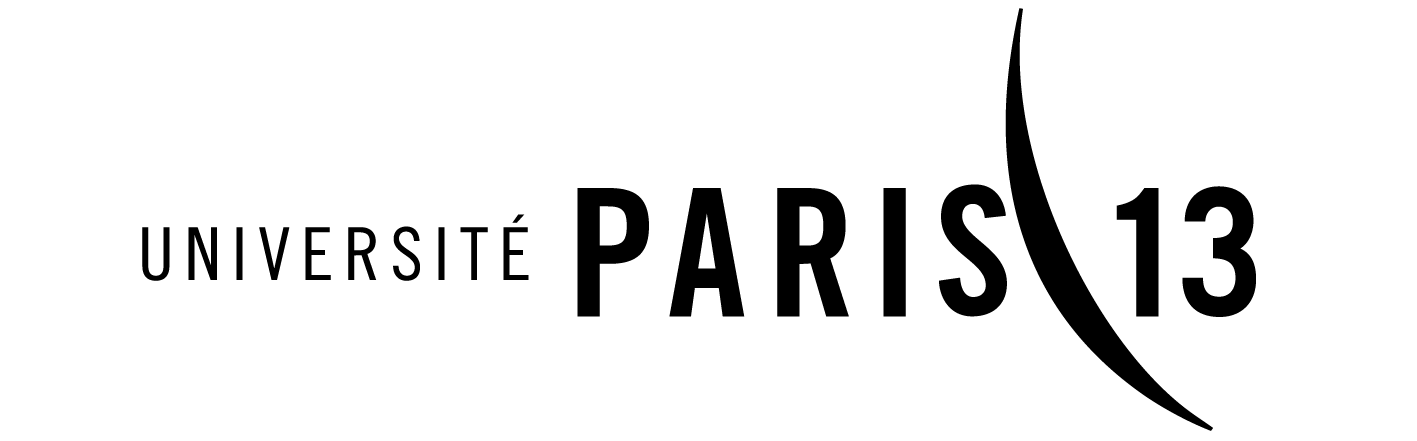
\includegraphics[height = 3cm]{images/logo/P13.png}
\hfill

\includegraphics[height = 3cm]{images/logo/laga.jpg}


\begin{center}
\vspace{\stretch{1}}
% Permet de créer un espace vertical de longueur variable (\stretch) et de "poids" 1
{\Large \textbf{École Doctorale 146 \\« Sciences, Technologies, Santé – Galilée »}}

\vspace{\stretch{2}}
%Espace vertical variable de poids 2.

{\Huge \textsc{Thèse de doctorat}}

\vspace{\stretch{1}}

{\LARGE Discipline: Mathématiques Appliquées}

\vspace{\stretch{3}}

{\large présentée par}
\vspace{\stretch{1}}

{
    \textbf{{\LARGE Pierre PAYEN}}\\
}

\vspace{\stretch{2}}
\hrule
\vspace{\stretch{1}}
{\LARGE \textbf{\doctitlefr}}
\vspace{\stretch{1}}
\hrule
% {\textbf{Version:} \hgid{}}
\vspace{\stretch{1}}

{\large dirigée par}
\vspace{\stretch{1}}

{
\large
    Pr.~Olivier LAFITTE (LAGA/Paris 13)\\
    et Dr.~Bruno STUPFEL (CEA)
}


\vspace{\stretch{5}}

{\Large Soutenue le XX/XX/XXXX devant le jury composé de :}

\vspace{\stretch{2}}
{\Large
\begin{tabular}{l@{\hskip 0cm}lll}
M\textsuperscript{me}.~&Xxxx \textsc{Xxxx} & Xxxx & Président\\
M.&Xxxx \textsc{Xxxx} & Xxxx & Rapporteur\\
M\textsuperscript{me}.&Xxxx \textsc{Xxxx} & Xxxx & Rapporteur\\
M.&Olivier \textsc{Lafitte} & LAGA/Paris 13 & Directeur\\
M.~&Bruno \textsc{Stupfel} & CEA & Examinateur\\
\end{tabular}
}

\end{center}
% \restoregeometry
% \cleardoublepage % pour laisser une page blanche au verso de la page de garde

\newpage
\thispagestyle{empty}
\vspace*{\fill}

%Adresse du labo où la thèse a été faite : demande du ministère !
\noindent
\begin{center}
\begin{minipage}[t]{0.5\textwidth}
LAGA - UMR 7539\\
Université Paris 13\\
99 avenue J.B. Clément\\
93430 Villetaneuse
\end{minipage}%
%
\hfill%
%
\begin{minipage}[t]{0.5\textwidth}
École doctorale 146 « Sciences, Technologies, Santé – Galilée »\\
Université Paris 13\\
99 avenue J.B. Clément\\
93430 Villetaneuse
\end{minipage}
\end{center}



\end{titlepage}
\hypersetup{pageanchor=true}
\cleardoublepage
    %     % Pages laminaires http://lettres.sorbonne-universite.fr/IMG/pdf/guide_redaction_d_une_these-2.pdf
% Elles contiennent :
% le résumé en français ; Le  résumé  doit  comporter  au  maximum  1700  caractères,  espaces compris.  Il  doit  être  précis  et  permettre  de  comprendre  comment  le  sujet  est  abordé.
% le titre en anglais ;
% le résumé en anglais ;
% les mots clés en français ;
% les mots clés en anglais ;
% l'intitulé et l'adresse de l'unité ou du laboratoire où la thèse a été présenté

\thispagestyle{empty}
\begin{center}
\Large
\textbf{\doctitlefr}
\end{center}
\section*{Résumé}
Nous considérons la diffraction électromagnétique d'un objet modélisé par une condition d'impédance (CI). L'originalité de cette thèse est l'établissement de nouvelles conditions suffisantes d'unicité (CSU) pour calculer les coefficients de cette condition limite et leur mise en œuvre dans un code équation intégrale. Cette modélisation est validée sur certains objets d'intérêt par comparaison avec des codes de référence.
\\

\textbf{Mots-clefs}


\dockeywordsfr

\hrulefill
\begin{center}
\Large
\textbf{\doctitleeng}
\end{center}
\section*{Abstract}
We consider the electromagnetic scattering from an object modelled by an impedance boundary condition (IBC). The originality of this thesis is the exhibition of sufficient uniqueness conditions (SUC) to compute the IBC coefficients and their implementation in a integral equation code. The approximated solution is then validated on some objects of interest.
\\

\textbf{Keywords}


\dockeywordseng

\chapterstar{Remerciement}
~{}

Ce manuscrit a été réalisé avec \(\LaTeXe\) dont les sources sont disponibles à \url{https://github.com/pirpyn/thesis}.
    %     \setcounter{secnumdepth}{5} % on numérote tous les niveaux de sections
    %     \setcounter{tocdepth}{1}  % Pas besoin de trop détailler le sommaire ici (chapitres/sections)
    %     \dominitoc
    %     \hypertarget{tableofcontent}{}%
    %     \pdfbookmark[0]{Sommaire}{tableofcontent}%
    %     \tableofcontents
    %     \newpage
\chapterstar{Acronymes et notations}
\TODO{Remplir l'index lorsque le manuscrit sera bien avancé}
% \setlength{\glsdescwidth}{\textwidth}
% \thispagestyle{empty}
% \printglossaries
% \thispagestyle{empty}

    %     \restoregeometry
    %%%%%%%%%%%%%%%%%%%%%%%%%%%%%%%%%%%%%%%%%%%%%%%%%
    \mainmatter
        \chapterstar{Introduction}
\section*{Présentation de la Thèse}\label{pre_th}
\lettrine{C}{ette} thèse de mathématiques appliquées s'intitule ``\doctitle''.
\\

L'objectif de la thèse est d’approfondir la notion de condition d'impédance pour des objets dont la surface est suffisamment régulière constitués d'empilement de matériaux diélectrique de faible indice (au sens de l'optique géométrique).
\\

L’intérêt des conditions d'impédances a été résumé par exemple par \cite{senior_approximate_1995}:
"Prenez par exemple, un objet fini immergé dans un milieu homogène et éclairé par un champ électromagnétique.
Connaissant les propriétés du matériau, il est possible en principe, de trouver les champ rayonnés à l'extérieur de l'objet.
Cependant, ce travail serait grandement facilité si les propriétés pouvait être modélisées par une condition limite ne faisant intervenir que la trace des champs à la surface extérieur de l'objet, de fait, transformant un problème à deux (ou plus) matériaux en un problème à un unique matériau.
"

\subsection*{Introduction}
Nous traitons le problème des équations Maxwell sous forme harmonique, en convention $e^{i\w t}$ pour la dépendance temporelle.


Soit un objet $\O$ de type conducteur parfait de surface $\Gamma$, recouvert d'une couche matériau diélectrique d'épaisseur $d$, caractérisé par sa permittivité diélectrique $\gls{phy-eps}$ et sa perméabilité magnétique $\gls{phy-mu}$ qui peuvent dépendre du point courant et être complexe dans le cas de pertes, l'ensemble se situant dans le vide, telle que la célérité d'une onde électromagnétique soit \gls{phy-c}, et les constantes de permittivité et de perméabilité $\gls{phy-eps}_0$, $\gls{phy-mu}_0$ avec $\eps_0\mu_0 = c^{2}$.


On désigne par \gls{phy-w} la pulsation de l'onde.
En l'absence de charges électriques et magnétiques, les champs éponymes $( \E, \H )$ sont solutions du système d'équations de Maxwell harmonique : 

Le problème de Maxwell dans l'espace s'énonce: \\

Soit $(\E,\H)$ dans $(\Hrot(\O\cup\O^c))^3 \pvect (\Hrot(\O\cup\O^c))^3$
\begin{equation}
\label{eq:pres_th:intro:maxwell}
\left\lbrace \begin{matrix}
\rot \E + i\w\mu' \H &=& 0 \\
\rot \H - i\w\eps' \E &=& 0 \\
\end{matrix} \right.
\quad \text{dans $\O\cup\O^c$}
\end{equation}
A l'extérieur de $\O$, les constantes sont $\eps',\mu'$ sont $\eps_0,\mu_0$ et à l'intérieur elles sont $\eps,\mu$.


Nous complétons ces équations par des conditions aux limites à la surface $S$ de $\O$, supposée régulière et dont on note la normale sortante $\n$:
\begin{itemize}
  \item Les composantes tangentielles des champs sont continues le long d'une surface de discontinuité de $\eps$ et $\mu$ \cite[(2.10) p.~8]{senior_approximate_1995}.

  \begin{align}
  \label{eq:pres_th:intro:transmissions}[\n \pvect \E]_S = 0  \qquad [\n \pvect \H]_S = 0
  \end{align}
\end{itemize}
Dans le cas limite d'un \gls{acr-cep}, les champs $\E$ et $\H$ sont nuls à l'intérieur du conducteur et la composante tangentielle (resp.normale) du champs $\E$ (resp.$\H$) est nulle à l'extérieur.


Enfin comme nous considérons un milieu extérieur non-borné, nous nous dotons de la condition de radiation à l'infini de Silver-Müller afin de définir des solutions en ondes sortantes.


\begin{equation}
\label{eq:pres_th:intro:silver-muller}
\lim_{r\rightarrow\infty}r\left|\left|\sqrt{\eps'}\E - \sqrt{\mu'}\H\pvect\frac{\v r}{r}\right|\right| = 0
\end{equation} 

\subsection*{Les conditions d'impédance comme approximation d'un opérateur de Calderón}

Tel que l'a démontré \cite[Theorem 1., p.~1042]{lafitte_diffraction_1998}, le problème \eqref{eq:pres_th:intro:maxwell}  posé à l'intérieur et à l'extérieur de l'objet, doté de la condition de rayonnement \eqref{eq:pres_th:intro:silver-muller} est équivalent au problème \eqref{eq:pres_th:intro:maxwell} à l'extérieur de l'objet doté de de la condition de rayonnement \eqref{eq:pres_th:intro:silver-muller} et de la \gls{acr-ci} \eqref{eq:pres_th:ci:ci-calderon} sur la surface extérieur de l'objet : 
\begin{equation}
\label{eq:pres_th:ci:ci-calderon}
\n \pvect \E = \mathcal{C}\left(\n \pvect \n \pvect \H\right)
\end{equation}
où $ \mathcal{C}$ est l'opérateur de Calderón.
L'opérateur d'impédance est alors une approximation de cet opérateur de Calderón.

% \subsection*{Plan de la thèse}
% D'abord nous résoudrons le problème de Maxwell dans le cas d'un plan infini recouvert d'une couche mince de matériau diélectrique.
Ce cas permet d'introduire et d'expliciter toutes les notions récurrentes de ce document.


% Puis nous résoudrons le problème de Maxwell avec un objet sphérique.
Pour cela, nous étudierons le problème de Helmholtz (section \ref{sec:helmholtz_scal}) avec un objet sphérique afin d'exhiber des solutions particulière de Maxwell (section \ref{sec:sol_maxwell}), dont nous détaillerons les champs sous la forme d'une série de Mie (section \ref{sec:serie_mie}).
Plusieurs calculs des termes principaux de cette série seront exhibés : solution exacte et injection des \glspl{acr-cioe}.
Ces dernières seront introduites en section  \ref{sec:coeffs_cioe}.


% Nous montrerons alors que l'on peut résoudre les équations de Maxwell grâce à la résolution d'équations intégrales, qui permettent de ne résoudre le problème qu'à la surface du domaine.


\setcounter{mtc}{2} % "Corrige" les minitocs décallés à cause des chapter* (ex : Intro)
        \chapter{Expression de l'opérateur pseudo-différentiel d'impédance}
%\citationChap{L'infini c'est long, surtout vers la fin}{Inconnu}
\minitoc
\begin{TODO}
    On explicite le symbole sur les coordonnées tangentielles. Or on a des champs 3D. Est-ce bien équivalent ?
\end{TODO}
\section{Analyse de Fourier de l'opérateur d'impédance}

Des résultat sur l'analyse spectrale de l'opérateur d'impédance ont déjà été présenté par \cite{hoppe_impedance_1995} pour des conducteurs plans et des cylindriques recouvert d'une couche de matériau.
Nous les rappellerons ainsi la méthode pour les obtenir puis nous expliciterons ces derniers à des matériaux multi-couches sur les même objets

% \TODO{
%     Généraliser ce qui suit à des matériaux non borné à l'aide de fonctions rapidement décroissantes
% }

Soit \(\OO\) un domaine fermé, bornée, de frontière régulière. Supposons que ces champs soient \(L^2\) en espace et en temps: \((\vE(\vect{x},t),\vH(\vect{x},t)) \in L^2(\OO \times \RR_+) \cap L^2(\OO^c\times\RR_+)\) et vérifient les équations de Maxwell:
\begin{equation}
    \left\lbrace 
    \begin{matrix}
    \vrot \vE(\vect{x},t) &=& -\mu(\vx) \ddr{t}{\vH}(\vx,t) \\
    \vrot \vH(\vect{x},t) &=& \eps(\vx) \ddr{t}{\vE}(\vx,t)
    \end{matrix}
    \right.
\end{equation}

On suppose aussi que \(\eps\) et \(\mu\) sont constant par morceaux.

Puisque ces champs \(\vE(\vect{x},t),\vH(\vect{x},t)\) sont \(L^2\), on peut définir leurs transformées de Fourier \(\hat{\vE}(\vect{k},\w), \hat{\vH}(\vect{k},\w)\) (\cite[Théorème de Plancherel, p.~153]{yosida_functional_1995}) telle que

\begin{equation}
    \hat{\vE} (\vect{k},\w) = \frac{1}{\sqrt{2\pi}^3}\int_{\RR^3\times\RR_+} e^{-i(\vect{k} \cdot \vect{x}+\w t)}\vE(\vect{x},t) \dd{x}\dd{t}\,, \quad \dd x = \prod\limits_{i=1}^3 \dd{x}_i
\end{equation}
\begin{equation}
    \vE(\vect{x},t) = \frac{1}{\sqrt{2\pi}^3}\int_{\RR^3\times\RR_+} e^{i(\vect{k} \cdot \vect{x}+\w t)}\hat{\vE} (\vect{k},\w) \dd{k} \dd{\w}\,, \quad \dd k = \prod\limits_{i=1}^3 \dd{k}_i
\end{equation}
La méthode pour trouver une expression de l'opérateur d'impédance est la suivante.
\begin{itemize}
\item Faire une transformée de Fourier partielle des champs, dépendante de la géométrie.
\item Réécrire le système d'équation de Maxwell simplifié.
\item Obtenir des EDO simple à résoudre sur les composantes des champs.
\item Utiliser les conditions limites pour obtenir les solutions particulières de cette EDO. 
\item En déduire l'opérateur d'impédance en Fourier.
\end{itemize}

Dans ce qui suit, on réalise au moins une transformée partielle en temps. La variable de Fourier associée est \(\w\), et donc l'opérateur \(\ddr{t}{~}\) est remplacé par \(i\w\).

% \begin{tcolorbox}
% On ne différencie pas les champs \(\vE,\vH\) de leurs transformées de Fourier \(\hat \vE, \hat \vH\).
% \end{tcolorbox}

On va donc utiliser le système d'équations de Maxwell harmonique:
\begin{equation}
    \left\lbrace 
    \begin{matrix}
    \vrot \hat \vE(\vx,\w)  &=& -i \omega \mu \hat \vH(\vx,\w)  \\
    \vrot \hat \vH(\vx,\w)  &=& i \omega \eps \hat \vE(\vx,\w) 
    \end{matrix}
    \right.
    \label{eq:imp_fourier:intro:maxwell_harmonique}
\end{equation}

A partir de maintenant, la dépendance en \(\w\) sera implicite: \(\hat \vE(\vx) \equiv \hat \vE (\vx, \w)\).
\section{Cas d'un objet plan infini}
    % Ce cas est très bien documenté (\cite{senior_approximate_x995},\cite{hoppe_impedance_x995}) et pose la méthodologie à adopter pour les objets courbes.

\begin{TODO}
    Corriger problème de signe
\end{TODO}

    \begin{figure}[!h]
        \begin{center}
            \begin{tikzpicture}
                \tikzmath{
    \largeur = 6;
    \hauteur = 1;
    \milieu = 1.3;
    \xC = \largeur;
    \xA = 0;
}

%% 1ere couche
\tikzmath{
    \yC = \hauteur;
    \yA = 0;
}

\coordinate (A) at (\xA,\yA);
\coordinate (B) at (\xA,\yC);
\coordinate (C) at (\xC,\yC);

\draw ($(B)!0.5!(C)$) node [above] {vide};


\fill [lightgray] (A) rectangle (C);
\draw ($(A)!0.5!(C)$) node {$\peps,\pmu,d$};
\draw (B) -- (C) node [right] {$\z = 0$};

%% Le repère
\tikzmath{
    \xD = \xC + 1.5;
}

\coordinate (n) at (\xD,\yA);

\draw [->] (n) -- ++(0,1) node [at end, right] {$\v{\z}$};
\draw [->] (n) -- ++(1,0) node [at end, right] {$\v{\x}$};

\draw (n) circle(0.1cm) node [below=0.1cm] {$\v{\y}$};
\draw (n) +(135:0.1cm) -- +(315:0.1cm);
\draw (n) +(45:0.1cm) -- +(225:0.1cm);

%% Le conducteur
\tikzmath{
    \yC = \yC - \hauteur;
    \yA = \yA - 0.5*\hauteur;
}

\coordinate (A) at (\xA,\yA);
\coordinate (B) at (\xA,\yC);
\coordinate (C) at (\xC,\yC);
\draw (B) -- (C);

\fill [pattern=north east lines] (A) rectangle (C);



            \end{tikzpicture}
        \end{center}
    \end{figure}

    Dans un premier temps, on peut sans perte de généralités faire une rotation du repère pour avoir le plan orthogonal à \(\vect{z}\). Comme il est infini dans les directions \(\vect{e_x} \vect{e_y}\) et que le matériau est homogène isotrope, on utilise la transformée partielle en \(x, y\) seulement.
    \begin{equation}
        \vE(x,y,z) = \frac{1}{2\pi}\iint_{\RR^2} e^{i(k_x x + k_y y)}\hat{\vE} (k_x,k_y,z) \dd{k_x}\dd{k_y}
    \end{equation}

    \begin{prop}
        Soient \(\vect{X}(k_x,k_z,z) =
        \begin{bmatrix}
        \hat{E_x} &
        \hat{E_y} &
        \hat{H_x} &
        \hat{H_y}
        \end{bmatrix}^t\),
        où \((\hat \vE,\hat \vH)\) sont des solutions du problème \eqref{eq:imp_fourier:intro:maxwell_harmonique}, alors il existe une matrice \(\mat{M}\) ne dépendant pas de \(z\) telle que
        \begin{equation}
            \ddr{z}{}\vect{X}(k_x,k_z,z) = \mat{M}(k_x,k_z) \vect{X}(k_x,k_z,z)
            \label{eq:imp_fourier:plan:edo}
        \end{equation}
    \end{prop}

    \begin{proof}
        En utilisant les multiplicateur de Fourier associés aux opérateurs différentiels, le problème \eqref{eq:imp_fourier:intro:maxwell_harmonique} s'écrit
        \begin{align*}
            \left\lbrace
            \begin{matrix}
            ik_y \hat{E_z}  - \ddr{z}{\hat{E_y}} = -i \w \mu \hat{H_x} \\
            \ddr{z}{\hat{E_x}} - ik_x \hat{E_z} = -i\w \mu \hat{H_y} \\
            ik_x \hat{E_y} - ik_y \hat{E_x} = -i\w \mu \hat{H_z} \\
            \end{matrix}
            \right. \quad
            \left\lbrace
            \begin{matrix}
            ik_y \hat{H_z}  - \ddr{z}{\hat{H_y}} = i \w \eps \hat{E_x} \\
            \ddr{z}{\hat{H_x}} - ik_x \hat{H_z} = i\w \eps \hat{E_y} \\
            ik_x \hat{H_y} - ik_y \hat{H_x} = i\w \eps \hat{E_z} \\
            \end{matrix}
            \right.
        \end{align*}

        Les composantes normales se déduisant des composantes tangentielles, on résout l'équation différentielle  matricielle à coefficients constants
        suivante \(\ddr{z}{}\vect{X} = \mat{M} \vect{X}\) où

        \begin{equation}
            \mat{M} = \begin{bmatrix}
            0 & 0 & -i\frac{k_xk_y}{\w\eps} & -i\left(\w\mu - \frac{k_x^2}{\w\eps}\right)\\
            0 & 0 & i\left(\w\mu - \frac{k_y^2}{\w\eps}\right) & i\frac{k_xk_y}{\w\eps}\\
            i\frac{k_xk_y}{\w\mu} & i\left(\w\eps - \frac{k_x^2}{\w\mu}\right) & 0 & 0 \\
            -i\left(\w\eps - \frac{k_y^2}{\w\mu}\right) & -i\frac{k_xk_y}{\w\mu} & 0 & 0 \\
            \end{bmatrix}
        \end{equation}
    \end{proof}

    \begin{prop}
        On définit
        \begin{equation}
            k_3=\sqrt{\w^2\eps\mu - k_x^2 -k_y^2} \quad \lambda_\pm=\pm i k_3
        \end{equation}
        \begin{equation}
            \vect{V_\pm} =
            \begin{bmatrix}
            \lambda_\pm \\
                0 \\
                -i\frac{k_xk_y}{\w\mu} \\
                i\left(\w\eps - \frac{k_y^2}{\w\mu}\right) \\
            \end{bmatrix}
            \quad
            \vect{W_\pm} =
                \begin{bmatrix}
                0 \\
                \lambda_\pm \\
                -i\left(\w\eps - \frac{k_x^2}{\w\mu}\right) \\
                i\frac{k_xk_y}{\w\mu} \\
            \end{bmatrix}
        \end{equation}
        alors
        \begin{subequations}
            \begin{align}
                \Ker(\mat{M}-\lambda_+\mI)=\Vect{\vect{V_+};\vect{W_+}}\\
                \Ker(\mat{M}-\lambda_-\mI)=\Vect{\vect{V_-};\vect{W_-}}
            \end{align}
        \end{subequations}
    \end{prop}

    \begin{proof}
        % Pour résoudre cette EDO, nous allons chercher les vecteurs propres \(V_i\) et les valeurs propres \(\lambda_i\) associées de ce système. En effet, une solution générale de ce système s'écrit
        % \begin{equation}
        %     \vect{X}(z)= \sum\limits_{i=1}^{4}c_i e^{\lambda_i z} \vect{V}_i \, c_i \in \CC
        % \end{equation}
        On pose
        \begin{equation*}
            \mat{A} = -\begin{bmatrix}
                i\frac{k_xk_y}{i\w\eps} & i\left(\w\mu - \frac{k_x^2}{\w\eps}\right) \\
                -i\left(\w\mu - \frac{k_y^2}{\w\eps}\right) & -i\frac{k_xk_y}{i\w\eps} \\
            \end{bmatrix}
            \quad
            \mat{B} = -\begin{bmatrix}
                -i\frac{k_xk_y}{\w\mu} & -i\left(\w\eps - \frac{k_x^2}{\w\mu}\right) \\
                i\left(\w\eps - \frac{k_y^2}{\w\mu}\right) & i\frac{k_xk_y}{\w\mu} \\
            \end{bmatrix}
        \end{equation*}
        Le déterminant de \(\mat{M}-\lambda \mat{I}\) est
        \begin{align*}
            \det(\mat{M}-\lambda \mat{I}) &=
            \begin{vmatrix}
                -\lambda \mI & \mA \\
                \mB & -\lambda \mI
            \end{vmatrix}
                = \frac{\det(- \lambda \mI - \mB(-\lambda \mI)^{-1} \mA)}{\det((-\lambda \mI)^{-1})} \\
                &= \det(\lambda^2 \mI - \mB\mA) \\
                &= (\lambda^2 + (\w^2\eps\mu - k_x^2 -k_y^2))^2 \\
                &= (\lambda^2 - \lambda_\pm^2)^2
        \end{align*}
        % On note alors
        % \begin{equation}
        % k_3=\sqrt{\w^2\eps\mu - k_x^2 -k_y^2}
        % \end{equation}

        % Les valeurs propres sont alors
        % \begin{equation}
        %     \lambda_\pm = \pm i k_3
        % \end{equation}
        % Les espaces propres associés sont de dimension 2, on a

        Par un calcul immédiat, on vérifie que \(\mat{M}\vect{V}_\pm = \lambda_\pm\vect{V}_\pm\) et \(\mat{M}\vect{W}_\pm = \lambda_\pm\vect{W}_\pm\).
    \end{proof}

    \begin{prop}
        On pose
        \begin{align}
            \mC &=
            \begin{bmatrix}
                \left(\w\eps-\frac{k_y^2}{\w\mu}\right) & \frac{k_xk_y}{\w\mu}\\
                \frac{k_xk_y}{\w\mu} & \left(\w\eps-\frac{k_x^2}{\w\mu}\right)
            \end{bmatrix}
        \end{align}
        alors
        \begin{subequations}
            \label{eq:imp_fourier:plan:champs}
            \begin{align}
                \begin{bmatrix}
                    \hat{E_x}(k_x,k_y,z)\\
                    \hat{E_y}(k_x,k_y,z)\\
                \end{bmatrix}
                &=ik_3\left( e^{ik_3 z}
                \begin{bmatrix}
                    c_1 \\
                    c_2
                \end{bmatrix}
                -e^{-ik_3 z}
                \begin{bmatrix}
                    c_3 \\
                    c_4
                \end{bmatrix}
                \right)
                \label{eq:imp_fourier:plan:champs:E}
                \\
                \begin{bmatrix}
                    -\hat{H_y}(k_x,k_y,z)\\
                    \hat{H_x}(k_x,k_y,z)\\
                \end{bmatrix}
                &=-i
                \mC
                \left(
                    e^{ik_3 z}
                    \begin{bmatrix}
                        c_1 \\
                        c_2
                    \end{bmatrix}
                    +e^{-ik_3 z}
                    \begin{bmatrix}
                        c_3 \\
                        c_4
                    \end{bmatrix}
                \right)
                \label{eq:imp_fourier:plan:champs:H}
            \end{align}
        \end{subequations}
    \end{prop}

    \begin{proof}
        On déduit des vecteur propres une solution générale de \eqref{eq:imp_fourier:plan:edo}.

        Soient \((c_i)_{i} \in \CC^4\)
        \begin{equation}
            \vect{X}(k_x,k_y,z) = c_1e^{\lambda_+ z}\vect{V_+}  + c_2e^{\lambda_+ z}\vect{W_+} + c_3e^{\lambda_- z}\vect{V_-} +c_4e^{\lambda_- z}\vect{W_-}
        \end{equation}

        On exprime \(\hat \vE_t(k_x,k_y,z)\) et \(\vect{e_z} \pvect \hat \vH_t(k_x,k_y,z)\)
        \begin{align}
            \begin{bmatrix}
                \hat{E_x}(k_x,k_y,z)\\
                \hat{E_y}(k_x,k_y,z)\\
            \end{bmatrix}
            &=
            \begin{bmatrix}
                c_1 e^{\lambda_+ z} \lambda_{+} + c_3 e^{\lambda_- z} \lambda_{-} \\
                c_2 e^{\lambda_+ z} \lambda_{+} + c_4 e^{\lambda_- z} \lambda_{-}
            \end{bmatrix}\\
            &=ik_3\left( e^{ik_3 z}
            \begin{bmatrix}
                c_1 \\
                c_2
            \end{bmatrix}
            -e^{-ik_3 z}
            \begin{bmatrix}
                c_3 \\
                c_4
            \end{bmatrix}
            \right)
        \end{align}

        \begin{align}
            \begin{bmatrix}
                -\hat{H_y}(k_x,k_y,z)\\
                \hat{H_x}(k_x,k_y,z)\\
            \end{bmatrix}
            &=
            \begin{bmatrix}
                -i\left(\w\eps - \frac{k_y^2}{\w\mu}\right) \left( c_1 e^{ik_3 z} + c_3 e^{-ik_3 z} \right) - i\frac{k_xk_y}{\w\mu} \left( c_2 e^{ik_3 z} + c_4 e^{-ik_3 z} \right)
                \\
                -i\frac{k_xk_y}{\w\mu} \left( c_1 e^{ik_3 z} + c_3 e^{-ik_3 z} \right) - i\left(\w\eps - \frac{k_x^2}{\w\mu}\right)\left( c_2 e^{ik_3 z} + c_4 e^{-ik_3 z} \right)
            \end{bmatrix} \\
            &=-i
            \mC
            \left(
                e^{ik_3 z}
                \begin{bmatrix}
                    c_1 \\
                    c_2
                \end{bmatrix}
                +e^{-ik_3 z}
                \begin{bmatrix}
                    c_3 \\
                    c_4
                \end{bmatrix}
            \right)
        \end{align}

        Comme \(\det(\mC) = k_3^2\frac{\eps}{\mu}=\frac{k_3^2}{\eta^2}\) alors une condition nécessaire pour trouver l'opérateur d'impédance est que \(k_3\) soit non nul ce qui aussi une hypothèse à vérifier car les valeurs propres doivent être non nulles.\footnote{\(k_3\) peut s'annuler pour des \(\eps,\mu\) réels.}.

    \end{proof}
    % On peut noter d'après \cite[eq.~(6)]{stupfel_2011}

    % \begin{equation}
    %     \mC^{-1}= \frac{\eta^2}{k_3^2}\left(k^2\mI - \mat{L_R}\right)
    %     \label{eq:imp_fourier:plan:C}
    % \end{equation}


    %%%%%%%%%%%%%%%%%%%%%%%%%%%%%%%%%%%%%%%%%%%%%%%%%%%%%%%%%%%%%%%%%%%%%%%
    %%%%%%%%%%%%%%%%%%%%%%%%%%%%%%%%%%%%%%%%%%%%%%%%%%%%%%%%%%%%%%%%%%%%%%%
    %%%%%%%%%%%%%%%%%%%%%%%%%%%%%%%%%%%%%%%%%%%%%%%%%%%%%%%%%%%%%%%%%%%%%%%


    \subsection{Opérateur d'impédance pour une couche}

        \begin{defn}
            On définit le symbole de l'opérateur d'impédance, la matrice \(\hat \mZ(k_x,k_y)\) tel que
            \begin{equation}
                \hat \vE_t(k_x,k_y,0) = \hat \mZ(k_x,k_y) \left(\vect{e_z} \pvect \hat \vH_t(k_x,k_y,0)\right)
            \end{equation}
        \end{defn}

        \begin{thm}
            Supposons que
            \begin{subequations}
                \label{eq:imp_fourier:plan:hyp_1_c}
                \begin{align}
                    k_3     & \not =0 \\
                    k_3d    & \not = \frac{\pi}{2}+n\pi\,, \forall n \in \NN
                \end{align}
            \end{subequations}

            Alors
            \begin{align}
            \label{eq:imp_plan:symb_z:1c}
            \hat \mZ(k_x,k_y) &= -i\eta\frac{\tan\left(k_3d\right)}{kk_3}
                \begin{bmatrix}
                   k^2-k_x^2  & -k_xk_y\\
                    -k_xk_y & k^2-k_y^2\\
                \end{bmatrix}
            \end{align}
        \end{thm}

        \begin{proof}
            Nous utilisons la condition limite
            \begin{equation}
                \begin{bmatrix}
                    \hat{E_x}(k_x,k_y,-d)\\
                    \hat{E_y}(k_x,k_y,-d)\\
                \end{bmatrix}
                =
                \begin{bmatrix}
                    0\\
                    0\\
                \end{bmatrix}
            \end{equation}

            De \eqref{eq:imp_fourier:plan:champs:E}, on déduit
            \begin{align}
                \begin{bmatrix}
                    c_1 \\
                    c_2
                \end{bmatrix}
                = e^{2ik_3 d}
                \begin{bmatrix}
                    c_3 \\
                    c_4
                \end{bmatrix}
            \end{align}

            En injectant ce qui précède dans \eqref{eq:imp_fourier:plan:champs}, on déduit que
            \begin{align}
                \begin{bmatrix}
                    \hat{E_x}(k_x,k_y,0)\\
                    \hat{E_y}(k_x,k_y,0)\\
                \end{bmatrix}
                &=ik_3\left( e^{i2k_3 d} -1 \right)
                \begin{bmatrix}
                    c_3 \\
                    c_4
                \end{bmatrix} \\
                \begin{bmatrix}
                    -\hat{H_y}(k_x,k_y,0)\\
                    \hat{H_x}(k_x,k_y,0)\\
                \end{bmatrix}
                & = - i\left(e^{i2k_3 d} +1 \right)
                \mC
                \begin{bmatrix}
                c_3 \\
                c_4
                \end{bmatrix}
            \end{align}

            En supposant \(k_3d \not = \frac{\pi}{2} + n\pi\), on déduit donc que
            \begin{align}
                \hat \mZ(k_x,k_y) &=  - k_3 \frac{e^{i2k_3d} -1}{e^{i2k_3d} +1} \mC^{-1}
                \\
                &= -\frac{\eta^2}{k_3} \frac{e^{i2k_3d} -1}{e^{i2k_3d} +1}
                    \begin{bmatrix}
                       \left(\w\eps-\frac{k_x^2}{\w\mu}\right)  & -\frac{k_xk_y}{\w\mu}\\
                        -\frac{k_xk_y}{\w\mu} &  \left(\w\eps-\frac{k_y^2}{\w\mu}\right)
                    \end{bmatrix}
                \\
                &= -i\eta\frac{\tan\left(k_3d\right)}{kk_3}
                    \begin{bmatrix}
                       k^2-k_x^2  & -k_xk_y\\
                        -k_xk_y & k^2-k_y^2\\
                    \end{bmatrix}
            \end{align}

        \end{proof}
        %On remarque que \(\det(\mat{Z}) = i\frac{\eta^2}{k_3}\eta\tan(k_3d)\) et donc pour un matériau \((\eps,\mu,d)\) donné, l'opérateur d'impédance n'est pas inversible pour tous  \((k_x,k_y) \in \RR^2, n \in \NN\), \(k_x^2+k_y^2 =  \w^2\eps\mu - \frac{1}{d^2}\left(\frac{\pi}{2} + n\pi\right)^2\), qui ne peut être vérifié que si \(\eps\mu\) est réel\footnote{Comme \(\eps, \mu\) sont à partie réelle (resp. imaginaire) strictement positive (resp. négative), alors ce n'est vrai pour les matériaux à partie imaginaire nulle.}.

        En pratique, on néglige toute les dépendance en \(y\) : \(k_y = 0\) ce qui revient à une propagation dans le plan \(xz\). Grâce à cette hypothèse, on trouve que \(\mC, \hat \mZ\) sont des matrices diagonales.

        De plus, on exprime souvent l'impédance selon la polarisation.
        Dans le cas plan, le champ \(\vE\)-TE correspond à \({E_y} \vect{e_y}\), le champ \(\vE\)-TM à \({E_x} \vect{e_x}\), tandis que le champ \(\vH\)-TM correspond à \({H_x} \vect{e_x}\) et le champ \(\vH\)-TE correspond à \({H_y} \vect{e_y}\).
        Dans ce cas, le symbole \(\hat \mZ\) peut se réécrire comme
        \begin{equation}
            \hat \mZ =
            \begin{bmatrix}
                \hat Z_{TM} & 0
                \\
                0 & \hat Z_{TE}
            \end{bmatrix}
        \end{equation}

    %%%%%%%%%%%%%%%%%%%%%%%%%%%%%%%%%%%%%%%%%%%%%%%%%%%%%%%%%%%%%%%%%%%%%%%
    %%%%%%%%%%%%%%%%%%%%%%%%%%%%%%%%%%%%%%%%%%%%%%%%%%%%%%%%%%%%%%%%%%%%%%%
    %%%%%%%%%%%%%%%%%%%%%%%%%%%%%%%%%%%%%%%%%%%%%%%%%%%%%%%%%%%%%%%%%%%%%%%

    \subsection{Opérateur d'impédance pour plusieurs couches}
        On suppose que l'on a \(n\) couches de matériaux :

        \begin{figure}[h!btp]
            \centering
            \begin{tikzpicture}
                \tikzmath{
    \largeur = 6;
    \hauteur = 0.5;
    \milieu = 1.3;
    \xC = \largeur;
    \xA = 0;
}

%% 1ere couche
\tikzmath{
    \yC = \hauteur;
    \yA = 0;
}

\coordinate (A) at (\xA,\yA);
\coordinate (B) at (\xA,\yC);
\coordinate (C) at (\xC,\yC);

\draw ($(B)!0.5!(C)$) node [above] {vide};


\fill [lightgray] (A) rectangle (C);
\draw ($(A)!0.5!(C)$) node {$\eps_n,\mu_n,d_n$};
\draw (B) -- (C) node [right] {$e_3 = 0$};

%% Des couches
\tikzmath{
    \yC = \yC - \hauteur;
    \yA = \yA - \milieu*\hauteur;
}

\coordinate (A) at (\xA,\yA);
\coordinate (B) at (\xA,\yC);
\coordinate (C) at (\xC,\yC);

\fill [lightgray]    (A) rectangle (C);
\fill [pattern=dots] (A) rectangle (C);
\draw (B) -- (C);

%% N ieme couche
\tikzmath{
    \yC = \yC - \milieu*\hauteur;
    \yA = \yA - \hauteur;
}

\coordinate (A) at (\xA,\yA);
\coordinate (B) at (\xA,\yC);
\coordinate (C) at (\xC,\yC);
\fill [lightgray] (A) rectangle (C);
\draw ($(A)!0.5!(C)$) node {$\eps_1,\mu_1,d_1$};
\draw (B) -- (C);

%% Le repère
\tikzmath{
    \xD = \xC + 0.5;
}

\coordinate (n) at (\xD,\yA);
\draw [->] (n) -- ++(1,0) node [at end, right] {$\v{e_1}$};
\draw [->] (n) -- ++(0,1) node [at end, right] {$\v{e_3}$};

\draw (n) circle(0.1cm) node [below=0.1cm] {$\v{e_2}$};
\draw (n) +(135:0.1cm) -- +(315:0.1cm);
\draw (n) +(45:0.1cm) -- +(225:0.1cm);

%% Le conducteur
\tikzmath{
    \yC = \yC - \hauteur;
    \yA = \yA - 0.5*\hauteur;
}

\coordinate (A) at (\xA,\yA);
\coordinate (B) at (\xA,\yC);
\coordinate (C) at (\xC,\yC);
\draw (B) -- (C);

\fill [pattern=north east lines] (A) rectangle (C);



            \end{tikzpicture}
        \end{figure}

        Pour chaque couche caractérisée par \((\eps_m,\mu_m,d_m)\), on définit:
        \begin{align}
        k_{3m} &= \sqrt{w^2\eps_m\mu_m - k_y^2 - k_x^2}
        \\
        \mC_m &=
            \begin{bmatrix}
                \left(\w\eps_m-\frac{k_y^2}{\w\mu_m}\right) & \frac{k_xk_y}{\w\mu_m}\\
                \frac{k_xk_y}{\w\mu_m} & \left(\w\eps_m-\frac{k_x^2}{\w\mu_m}\right)
            \end{bmatrix}
        \end{align}

        On rappelle que \(\det{\mC_m} = \frac{k_{3m}\eps_m^2}{\mu_m^2}\)

        On définit aussi la profondeur de la couche \(m\), \(l_m = -\sum_{i=0}^{n-m} d_{n-i} \).

        \begin{defn}
            On définit pour chaque interface, le symbole \(\hat \mZ_m\) tel que
            \begin{equation}
                \hat \vE_t(k_x,k_y,l_m) = \hat \mZ_m(k_x,k_y) \left(\vect{e_z} \pvect \hat \vH_t(k_x,k_y,l_m)\right)
            \end{equation}
        \end{defn}

        \begin{thm}
            Soit \(\hat \mZ_0(k_x,k_y) = \mat{0}_{\mathcal{M}_2(\CC)}\).

            Si pour tout \(0<m < n\)
            \begin{align}
                k_{3m} &\not = 0 \\
                \det\left(k_{3m}\mI \pm \hat \mZ_{m-1}\mC_m \right) &\not = 0 \\
                k_{3m}d_m &\not = \frac{\pi}{2}+n\pi\,, \forall n \in \NN \\
                \det\left(k_{3m}\mI - i\tan(k_{3m}d_m)\mZ_{m-1}\mC_m\right) &\not = 0
            \end{align}
            Alors le symbole \(\hat \mZ_n\) est défini par la relation de récurrence :
            \begin{multline}
                \hat \mZ_m = -k_{3m}
                \left(ik_{3m}\tan\left(k_{3m}d_m\right)\mI - \hat \mZ_{m-1}\mC_m\right) \\
                \left(k_{3m}\mI - i\tan\left(k_{3m}d_m\right)\hat \mZ_{m-1}\mC_m\right)^{-1}
                \mC_m^{-1}
            \end{multline}
        \end{thm}

        \begin{proof}
            À l'initialisation, la condition limite sur le conducteur impose \(\hat \mZ_0 = \mat{0}_{\mathcal{M}_2(\CC)}\) et on retrouve le résultat pour une couche.

            Par récurrence, un empilement à \(n\) couches se ramène à un empilement à une couche avec la condition:
            \begin{equation}
                \begin{bmatrix}
                    \hat{E_x}(k_x,k_y,-d)\\
                    \hat{E_y}(k_x,k_y,-d)\\
                \end{bmatrix}
                =
                \mZ_m
                \begin{bmatrix}
                    -\hat{H_y}(k_x,k_y,-d)\\
                    \hat{H_x}(k_x,k_y,-d)\\
                \end{bmatrix}
            \end{equation}

            On reprend donc tous les résultats de la partie précédente. Notamment, de \eqref{eq:imp_fourier:plan:champs:E} et \eqref{eq:imp_fourier:plan:champs:H}, on déduit que

            \begin{equation}
                \begin{bmatrix}
                    \hat{E_x}(k_x,k_y,-d)\\
                    \hat{E_y}(k_x,k_y,-d)\\
                \end{bmatrix}
                = ik_3\left( e^{-ik_3 d}
                \begin{bmatrix}
                    c_1 \\
                    c_2
                \end{bmatrix}
                -e^{ik_3 d}
                \begin{bmatrix}
                    c_3 \\
                    c_4
                \end{bmatrix}
                \right)
            \end{equation}

            \begin{equation}
                \begin{bmatrix}
                    -\hat{H_y}(k_x,k_y,-d)\\
                    \hat{H_x}(k_x,k_y,-d)\\
                \end{bmatrix}
                =-i
                \mC
                \left(
                    e^{-ik_3 d}
                    \begin{bmatrix}
                        c_1 \\
                        c_2
                    \end{bmatrix}
                    +e^{ik_3 d}
                    \begin{bmatrix}
                        c_3 \\
                        c_4
                    \end{bmatrix}
                \right)
            \end{equation}

            \begin{equation}
                ik_3\left( e^{-ik_3 d}
                \begin{bmatrix}
                    c_1 \\
                    c_2
                \end{bmatrix}
                -e^{ik_3 d}
                \begin{bmatrix}
                    c_3 \\
                    c_4
                \end{bmatrix}
                \right)
                =-i\hat\mZ_m\mC
                \left(
                    e^{-ik_3 d}
                    \begin{bmatrix}
                        c_1 \\
                        c_2
                    \end{bmatrix}
                    +e^{ik_3 d}
                    \begin{bmatrix}
                        c_3 \\
                        c_4
                    \end{bmatrix}
                \right)
            \end{equation}

            \begin{equation}
                \left(k_3\mI + \hat\mZ_m\mC\right)
                \begin{bmatrix}
                    c_1 \\
                    c_2
                \end{bmatrix}
                = e^{i2k_3 d} \left(k_3\mI - \hat\mZ_m\mC\right)
                \begin{bmatrix}
                    c_3 \\
                    c_4
                \end{bmatrix}
            \end{equation}

            On pose
            \begin{align}
                \mA_\pm &= k_3\mI \pm \hat\mZ_m\mC
            \end{align}

            On remarque que par définition, \(\mA_+\) et \(\mA_-\) commutent.

            Pour continuer il faut exprimer un vecteur en fonction de l'autre. On suppose donc \(\pm k_3\) ne sont pas des valeurs propres de \(\hat\mZ_m\mC\) et l'on déduit que

            \begin{align}
                \begin{bmatrix}
                    c_1 \\
                    c_2
                \end{bmatrix}
                &= e^{i2 k_3 d} \mA_+^{-1}\mA_-
                \begin{bmatrix}
                    c_3 \\
                    c_4
                \end{bmatrix}
                \\
                & = \mat{F}
                \begin{bmatrix}
                    c_3 \\
                    c_4
                \end{bmatrix}
            \end{align}

            \begin{align}
                \begin{bmatrix}
                    \hat{E_x}(k_x,k_y,0)\\
                    \hat{E_y}(k_x,k_y,0)\\
                \end{bmatrix}
                &=ik_3\left(\mat{F} - \mI \right)
                \begin{bmatrix}
                    c_3 \\
                    c_4
                \end{bmatrix}\\
                \begin{bmatrix}
                    -\hat{H_y}(k_x,k_y,0)\\
                    \hat{H_x}(k_x,k_y,0)\\
                \end{bmatrix}
                &=-i\mC \left(\mat{F} + \mI \right)
                \begin{bmatrix}
                        c_3 \\
                        c_4
                \end{bmatrix}
            \end{align}

            On suppose qu'en plus de \(\mA_+\) et \(\mA_-\), \(\mat{F} + \mI\) est inversible, on va utiliser la commutativité de \(\mA_+\) et \(\mA_-\).

            Alors le symbole \(\hat \mZ\) s'exprime

            \begin{align}
                \hat{\mat{Z}}_{m+1}
                &=-k_3\left(\mat{F} - \mI \right)\left(\mat{F}+ \mI \right)^{-1}\mC^{-1}
                \\
                &=-k_3\mA_+^{-1}\left(e^{i2 k_3 d}\mA_- - \mA_+ \right)\left(e^{i2 k_3 d}\mA_- + \mA_+ \right)^{-1}\mA_+\mC^{-1}
                \\
                &= -k_3\left( e^{i2 k_3 d} \mA_- -  \mA_+\right)
                \left( e^{i2 k_3 d} \mA_- + \mA_+ \right)^{-1}\mC^{-1}
                \\
                &= -k_3\left(\left( e^{i2 k_3 d} - 1 \right)\mI - \left( e^{i2 k_3 d} + 1 \right) \hat\mZ_m\mC \right)
                \left( \left( e^{i2 k_3 d} + 1 \right)\mI - \left( e^{i2 k_3 d} - 1 \right)\hat\mZ_m\mC \right)^{-1}\mC^{-1}
            \end{align}

            En supposant que \(\forall n \in \NN \,, k_3d\not = \frac{\pi}{2}+n\pi\), on a

            \begin{equation}
                \hat\mZ_{m+1} = -k_3\left(ik_3\tan(k_3 d)\mI - \hat\mZ_m\mC \right)
                    \left( k_3\mI - i\tan(k_3 d)\hat\mZ_m\mC \right)^{-1}\mC^{-1}
            \end{equation}

            % à condition que
            % \begin{align}
            %     \det\left(k_3\mI \pm \hat\mZ_m\mC \right) \not = 0 \\
            %     k_3d\not = \frac{\pi}{2}+n\pi\,, \forall n \in \NN \\
            %     \det\left(k_3\mI - i\tan(k_3d)\hat\mZ_m\mC\right) \not = 0
            % \end{align}

        \end{proof}

    %%%%%%%%%%%%%%%%%%%%%%%%%%%%%%%%%%%%%%%%%%%%%%%%%%%%%%%%%%%%%%%%%%%%%%%
    %%%%%%%%%%%%%%%%%%%%%%%%%%%%%%%%%%%%%%%%%%%%%%%%%%%%%%%%%%%%%%%%%%%%%%%
    %%%%%%%%%%%%%%%%%%%%%%%%%%%%%%%%%%%%%%%%%%%%%%%%%%%%%%%%%%%%%%%%%%%%%%%

    \subsection{Applications numériques}

        La figure \ref{fig:imp_fourier:plan:hoppe} permet de vérifier les résultats de \cite[p.~33]{hoppe_impedance_1995} pour une couche de matériau sans perte. On remarque que pour \(s=2\), \(k_3 = 0\) et donc \(\mC\) n'est pas inversible.

        \begin{figure}[!hbt]
            \centering
            \begin{tikzpicture}[scale=1]
                \begin{axis}[
                        title={},
                        ylabel={\(\Im(\hat{\mZ}(k_x,0)\)},
                        xlabel={\(k_x\slash k_0\)},
                        width=0.8\textwidth,
                        xmin=0,
                        xmax=2,
                        mark repeat=20,
                        legend pos=outer north east
                    ]
                    \legend{TM,TE}
                    \addplot [black] table [col sep=semicolon, x={s}, y={imag(z.tm)}] {tikz/csv/impedance/plan/HOPPE_33/hoppe_p33.csv};
                    \addplot [black,dashed] table [col sep=semicolon, x={s}, y={imag(z.te)}] {tikz/csv/impedance/plan/HOPPE_33/hoppe_p33.csv};
                \end{axis}
            \end{tikzpicture}
            \caption[Reproduction résultat Hoppe & Rahmat-Samii p.~33]{\(\eps = 4, \mu = 1, d=0.015\text{m}, f=1\text{GHz}\)}
            \label{fig:imp_fourier:plan:hoppe}
        \end{figure}

        La figure \ref{fig:imp_fourier:plan:soudais} permet de vérifier les résultats de \cite{soudais_3d_2017} pour une couche de matériau sans perte où \(k_3d = \frac{\pi}{2}\) pour \(k_x \simeq 0.9 k_0\).

        \begin{figure}[!hbt]
            \centering
            \begin{tikzpicture}[scale=1]
                \begin{axis}[
                        title={},
                        width=0.4\textwidth,
                        xmin=0,
                        xmax=2,
                        ylabel={\(\Im(\hat{\mZ}(k_x,0))\)},
                        xlabel={\(k_x\slash k_0\)},
                        mark repeat=20,
                        legend pos=outer north east
                    ]
                    \addplot [black] table [x={s}, y={imag(z.tm)},col sep=semicolon] {tikz/csv/impedance/plan/soudais.csv};
                    \addplot [black,dashed] table [x={s}, y={imag(z.te)},col sep=semicolon] {tikz/csv/impedance/plan/soudais.csv};
                \end{axis}
            \end{tikzpicture}
            \begin{tikzpicture}[scale=1]
                \begin{axis}[
                        title={},
                        width=0.4\textwidth,
                        ymin=-100,
                        ymax=100,
                        xmin=0.8,
                        xmax=1,
                        ylabel={},
                        xlabel={\(k_x\slash k_0\)},
                        mark repeat=20,
                        legend pos=outer north east
                    ]
                    \legend{TM,TE}
                    \addplot [black] table [x={s}, y={imag(z.tm)},col sep=semicolon] {tikz/csv/impedance/plan/soudais_zoom.csv};
                    \addplot [black,dashed] table [x={s}, y={imag(z.te)},col sep=semicolon] {tikz/csv/impedance/plan/soudais_zoom.csv};
                \end{axis}
            \end{tikzpicture}
            \caption[Reproduction résultat P. Soudais]{\(\eps = 4, \mu = 1, d=0.035\text{m}, f=12\text{GHz}\)}
            \label{fig:imp_fourier:plan:soudais}
        \end{figure}

        % \begin{figure}[!hbt]
        %     \begin{tikzpicture}
        %         \begin{axis}
        %             \addplot[%
        %                 contour prepared,%
        %                 contour prepared format=matlab%
        %             ] table {
        %                 % (0.2,6) ==> contour `0.2' (x), 5 points follow (y):
        %                 0.3000000e+00 6.0000000e+00
        %                 3.0000000e+00 4.0000000e-01
        %                 2.0000000e+00 2.8571429e-01
        %                 1.0000000e+00 3.3333333e-01
        %                 3.3333333e-01 1.0000000e+00
        %                 2.8571429e-01 2.0000000e+00
        %                 3.3333333e-01 3.0000000e+00
        %                 % (0.4,5) ==> contour `0.4', consists of 5 points
        %                 4.0000000e-01 5.0000000e+00
        %                 3.0000000e+00 8.0000000e-01
        %                 2.0000000e+00 5.7142857e-01
        %                 1.0000000e+00 6.6666667e-01
        %                 6.6666667e-01 1.0000000e+00
        %                 5.7142857e-01 2.0000000e+00
        %                 % (0.6,6) ==> contour `0.6', has 6 points
        %                 6.0000000e-01 6.0000000e+00
        %                 2.6666667e+00 2.0000000e+00
        %                 2.5000000e+00 1.0000000e+00
        %                 2.0000000e+00 8.5714286e-01
        %                 1.0000000e+00 1.0000000e+00
        %                 1.0000000e+00 1.0000000e+00
        %                 8.5714286e-01 2.0000000e+00
        %             };
        %         \end{axis}
        %     \end{tikzpicture}
        % \end{figure}

        % \def\tmpfile{graphes.txt}
        % \immediate\write18{rm -rf "\tmpfile"}
        % \immediate\write18{touch "\tmpfile"}
        % \immediate\write18{date >> "\tmpfile"}
        % \immediate\write18{gnuplot --version >> "\tmpfile"}
        % \begin{figure}[!hbt]
        %     \begin{tikzpicture}
        %         \begin{axis}
        %             \addplot3[
        %                 mesh/rows=4,
        %                 mesh/num points=12,
        %                 contour gnuplot={
        %                     number=5,
        %                     % cdata should not be affected by z filter:
        %                     output point meta=rawz,
        %                     labels=false,
        %                 }
        %             ] table [x index={1}, y index={2}, z index={3},col sep=comma] {
        %             1,-6.2832,-6.2832,0.74038,
        %             2,-6.2832,-6.1563,0.74997,
        %             3,-6.2832,-6.0293,0.75982,
        %             4,-6.2832,-5.9024,0.76986,
        %             5,-16.2832,-16.2832,10.74038,
        %             6,-16.2832,-16.1563,10.74997,
        %             7,-16.2832,-16.0293,10.75982,
        %             8,-16.2832,-15.9024,10.76986,
        %             9,-26.2832,-26.2832,20.74038,
        %             10,-26.2832,-26.1563,20.74997,
        %             11,-26.2832,-26.0293,20.75982,
        %             12,-26.2832,-25.9024,20.76986,
        %             };
        %         \end{axis}
        %     \end{tikzpicture}
        % \end{figure}
\section{Cas d'un objet cylindrique}

    % On rappelle les formules des opérateurs $\vdiv, \vrot$ en coordonnée cylindrique $(r,\theta,z)$.
    % \begin{align}
    %     \vrot \v{V} &= \left(\frac{1}{r}\ddr{\theta}{V_z} - \ddr{z}{V_\theta}\right)\v{e_r} + 
    %     \left(\ddr{z}{V_r} - \ddr{r}{V_z}\right)\v{e_\theta} +
    %     \frac{1}{r}\left(\ddr{r}{(rV_\theta)}-\ddr{\theta}{V_r}\right)\v{e_z} 
    %     \\
    %     \vdiv \v{V} &= \frac{1}{r}\ddr{r}{(rV_r)}+\frac{1}{r}\ddr{\theta}{V_\theta}+\ddr{z}{V_z}
    %     \\
    %     \vgrad f &= \ddr{r}{f}\v{e_r}
    %     +\frac{1}{r}\ddr{\theta}{f}\v{e_\theta} + \ddr{z}{f}\v{e_z}
    % \end{align}

    \begin{figure}[!hbt]
        \centering
        \begin{tikzpicture}
            \coordinate (mat) at (0,-1.5);
\coordinate (vide) at (0,-2);
\coordinate (c) at (0,0);

\fill [lightgray] (c) circle (2);
\fill [white] (c) circle (1.5);
\fill [pattern=north east lines] (c) circle (1.5);

\draw (c) circle (2);
\draw (c) circle (1.5);


\coordinate (n) at (0,2);

%\draw (vide) node [below] {$\eps_0,\mu_0$};
\draw (mat) node [below] {$\peps,\pmu$};

% Axess
\draw [->] (n) -- ++(0,1) node [at end, right] {$\v{\mr}$};
\draw [->] (n) -- ++(1,0) node [at end, right] {$\v{\mt}$};

\draw (n) ++(0.2,0.2) circle(0.1cm) node [above=0.1cm] {$\v{\mz}$};
\draw (n) ++(0.2,0.2) +(135:0.1cm) -- +(315:0.1cm);
\draw (n) ++(0.2,0.2) +(45:0.1cm) -- +(225:0.1cm);

%\draw [->>,thick] (lt) ++ (1,1) -- (mt) ;


        \end{tikzpicture}
    \end{figure}

    On exprime les équations de Maxwell dans le matériau dans la base cylindrique et sans pertes de généralité, on peut réaliser une transformée de Fourier en $z$ par invariance en translation et en $\theta$ par invariance en rotation. Cependant, le multiplicateur de Fourier associé à la coordonnée $\theta$ doit être un entier pour assurer la périodicité. On le note $n$.

    \begin{equation}
        \vE(r,\theta,z) = \frac{1}{2\pi}\sum_{i=-\infty}^{\infty}\int_{\RR} e^{i(n \theta + k_z z )}\hat{\vE} (r,n,k_z) \dd{k_z}
    \end{equation}

    \begin{prop}
        Soit
        \begin{equation}
            k_3 = \sqrt{\w^2\eps\mu - k_z^2}
        \end{equation}
        et $J_n$ et $H_n^{(2)}$ des solutions de l'équation de Bessel d'ordre $n$.
        
        Alors $\exists (c_1,c_2,c_3,c_4) \in \CC^4$ tels que la 3\ieme composante des champs soit
        \begin{subequations}
            \begin{align}
                \hat{E_z}(r,n,k_z) &= c_1 J_n\left(k_3r\right) + c_2 H_n^{(2)}\left(k_3r\right)
                \\
                \hat{H_z}(r,n,k_z) &= c_3 J_n\left(k_3r\right) + c_4 H_n^{(2)}\left(k_3r\right)
            \end{align}
        \end{subequations}
    \end{prop}

    \begin{proof}

        On peut simplifier les opérateurs différentiels:

        \begin{align}
            \vrot \hat \vE(r,n,k_z) &= i\left(\frac{n}{r}\hat{E_z} - k_z\hat{E_\theta}\right)\v{e_r} + 
            \left(ik_z\hat{E_r} - \ddr{r}{\hat{E_z}}\right)\v{e_\theta} +
            \frac{1}{r}\left(\ddr{r}{(r\hat{E_\theta})}-in\hat{E_r}\right)\v{e_z}
            \\
            &=i\w\mu \hat \vH(r,n,k_z)
        \end{align}

        On remarque que la méthode utilisée pour le plan aboutie à une équation différentielle à coefficients non constant de type $r\ddr{r}{X}(r,n,k_z) = M(r,n,k_z)X(r,n,k_z)$. On ne peut pas exprimer la solution avec les valeurs et vecteurs propres de la matrice. 
        %Nous allons donc trouver une équation de Bessel en développant le système de Maxwell.
        On développe le système de Maxwell:

        \begin{align}
            \vrot \vrot \hat \vE &= \w^2\eps\mu \hat \vE
            \\
            \vdiv \hat \vE &= 0
        \end{align}

        \begin{multline}
            \vrot \vrot \hat \vE = \dots\\
            i\left(\frac{n}{r^2}\left(\ddr{r}{(r\hat{E_\theta})} - in\hat{E_r}\right) - k_z\left(ik_z\hat{E_r} - \ddr{r}{\hat{E_z}}\right)\right)    \v{e_r} \dots\\ 
            + \left(-k_z\left(\frac{n}{r}\hat{E_z} - k_z\hat{E_\theta}\right) -\ddr{r}{}\left(\frac{1}{r}\left(\ddr{r}{(r\hat{E_\theta})}-in\hat{E_r}\right)\right)\right)    \v{e_\theta} \dots\\
            + \frac{1}{r}\left(\ddr{r}{} \left(r\left(ik_z\hat{E_r} - \ddr{r}{\hat{E_z}}\right)\right) + n \left(\frac{n}{r}\hat{E_z} - k_z\hat{E_\theta}\right)\right) \v{e_z}
        \end{multline}

        On aboutit au système suivant
        \begin{equation}
            \left\lbrace
            \begin{array}{ccc}
                -\left(\w^2\eps\mu -\frac{n^2}{r^2}  - k_z^2\right)\hat{E_r}  +i\frac{n}{r^2}\ddr{r}{(r\hat{E_\theta})}  +k_z\ddr{r}{\hat{E_z}} & = & 0\\
                in\ddr{r}{}\left(\frac{\hat{E_r}}{r}\right) -\left(\w^2\eps\mu - k_z^2\right)\hat{E_\theta} + \ddr{r}{}\left(\frac{1}{r}\ddr{r}{(r\hat{E_\theta})}\right)  - n\frac{k_z}{r}\hat{E_z} & = & 0\\
                i\frac{k_z}{r}\ddr{r}{(r\hat{E_r})}  - n\frac{k_z}{r}\hat{E_\theta}  -\left(\w^2\eps\mu - \frac{n^2}{r^2} \right)\hat{E_z} - \frac{1}{r}\ddr{r}{}\left(r\ddr{r}{\hat{E_z}}\right) & = & 0
            \end{array}
            \right.
        \end{equation}

        Comme l'on cherche $\hat \vE_t, \hat \vH_t$, on remarque que les 2\ieme composantes des équations de Maxwell permettent de déduire $\hat\vE_t, \hat\vH_t$ de $ \hat E_z, \hat H_z$

        De la troisième  équation, on trouve pour $r\not=0$
        \begin{equation}
        r^2 \ddr[2]{r}{\hat{E_z}} + r\ddr{r}{\hat{E_z}} + \left(r^2\w^2\eps\mu - n^2\right)\hat{E_z} =ik_zr\ddr{r}{(r\hat{E_r})} -  nk_zr\hat{E_\theta}
        \end{equation}

        Or comme $\vdiv \hat \vE = i\w\mu\vdiv\vrot \hat \vH = 0$, on a
        \begin{align}
            \vdiv\hat \vE &= \frac{1}{r}\ddr{r}{(r\hat{E_r})} + \frac{in}{r}\hat{E_\theta} + ik_z\hat{E_z}
            \\
            &=0
            \\
            k_z^2r^2 \hat{E_z} &= ik_zr\ddr{r}{(r\hat{E_r})} - nk_zr\hat{E_\theta}
        \end{align}

        On obtient donc sur la composante $\hat{E_z}$:
        \begin{equation}
            r^2 \ddr[2]{r}{\hat{E_z}} + r\ddr{r}{\hat{E_z}} + \left(r^2\left(\w^2\eps\mu - k_z^2\right) - n^2\right)\hat{E_z} = 0
        \end{equation}

        C'est une équation de Bessel (cf \cite[eq (6.80)]{bowman_introduction_1958}), dont des solutions générales sont: soient $(c_1,c_2) \in \CC^2$:
       \begin{equation}
            \hat{E_z}(r,n,k_z) = c_1 J_n\left(k_3r\right) + c_2 H_n^{(2)}\left(k_3r\right)
        \end{equation}
        où $J_n$ est la fonction de Bessel du premier type, $H_n^{(2)}$ la fonction de Hankel de deuxième type. On sait que l'on peut prendre n'importe quel couple de fonctions de Bessel (cf \eqref{eq:annex:bessel:equiv_bessel}), on choisit ce dernier car les $J_n$ sont régulières et les $H_n$ évoluent en $\frac{1}{\sqrt{r}}$ à l'infini, donc ce choix est adapté à une décomposition en une onde incidente partout définie et une onde réfléchie décroissante à l'infini.

        De plus, d'après \cite[p.~358]{abramowitz_handbook_1964}, on sait qu'une fonction de Bessel d'ordre $n$ est linéairement dépendante de celle d'ordre $-n$. On peut donc se restreindre à $n$ entier naturel

        On trouve exactement le même résultat pour $\hat{H_z}$: soient $(c_3,c_4) \in \CC^2$
        \begin{equation}
            \hat{H_z}(r,n,k_z) = c_3 J_n\left(k_3r\right) + c_4 H_n^{(2)}\left(k_3r\right)
        \end{equation}
    \end{proof}


    \newcommand{\mJ}{\mat{J}}
    \newcommand{\mH}{\mat{H}}

    \begin{defn}
        On définit les matrices $\mJ_{E}(r,n,k_z),\mH_{E}(r,n,k_z),\mJ_{H}(r,n,k_z),\mH_{H}(r,n,k_z)$
        \begin{align}
            \mJ_{E}(r,n,k_z) &= 
            \begin{bmatrix}
                -\frac{nk_z}{rk_3^2}J_n(k_3r) & -\frac{i\w\mu}{k_3}J_n'(k_3r)
                \\
                J_n(k_3r) & 0
            \end{bmatrix}
            \\
            \mH_{E}(r,n,k_z) &= 
            \begin{bmatrix}
                -\frac{nk_z}{rk_3^2}H_n^{(2)}(k_3r) & -\frac{i\w\mu}{k_3}H_n^{(2)}{}'(k_3r)
                \\
                H_n^{(2)}(k_3r) & 0
            \end{bmatrix}
            \\
            \mJ_{H}(r,n,k_z) &= 
            \begin{bmatrix}
                0 & -J_n(k_3r)
                \\
                \frac{i\w\eps}{k_3}J_n'(k_3r) & -\frac{nk_z}{rk_3^2}J_n(k_3r)
            \end{bmatrix}
            \\
            \mH_{H}(r,n,k_z) &= 
            \begin{bmatrix}
                0 & -H_n^{(2)}(k_3r)
                \\
                \frac{i\w\eps}{k_3}H_n^{(2)}{}'(k_3r) & -\frac{nk_z}{rk_3^2}H_n^{(2)}(k_3r)
            \end{bmatrix}
        \end{align}
    \end{defn}

    \begin{prop}
        Alors les champs tangentiels s'écrivent
        \begin{subequations}
            \begin{align}
                \hat \vE_t(r,n,k_z) &= \mJ_{E}(r,n,k_z)
                \begin{bmatrix}
                    c_1 \\
                    c_3
                \end{bmatrix}
                +
                \mH_{E}(r,n,k_z)
                \begin{bmatrix}
                    c_2 \\
                    c_4
                \end{bmatrix}
                \label{eq:imp_fourier:cylindre:Et}\\
                \v{e_r}\times\hat \vH_t(r,n,k_z) &= 
                \mJ_{H}(r,n,k_z)
                \begin{bmatrix}
                    c_1 \\
                    c_3
                \end{bmatrix}
                +
                \mH_{H}(r,n,k_z)
                \begin{bmatrix}
                    c_2 \\
                    c_4
                \end{bmatrix}
                \label{eq:imp_fourier:cylindre:Ht}
            \end{align}
        \end{subequations}
    \end{prop}


    \begin{proof}
        À partir des équations de Maxwell restantes, on peut déterminer $\hat{E_r},\hat{E_\theta},\hat{H_r},\hat{H_\theta}$.
        \begin{equation}
            \left\lbrace
            \begin{matrix}
                -ik_z\hat{E_\theta} - i\w\mu \hat{H_r} = -\frac{in}{r}\hat{E_z}
                \\
                ik_z\hat{E_r} - i\w\mu \hat{H_\theta} = \ddr{r}{\hat{E_z}}
                \\
                -i\w\eps \hat{E_r} + ik_z \hat{H_\theta} = \frac{in}{r}\hat{H_z}
                \\
                -i\w\eps \hat{E_\theta} - ik_z \hat{H_r} = -\ddr{r}{\hat{H_z}}
            \end{matrix}
            \right.
        \end{equation}

        Cela revient à résoudre $\v{Y} = \mat{M}\v{X}$ où la matrice $\mat{M}$ et les vecteurs $\v{X}, \v{Y}$ sont définis tels que
        \begin{equation}
            \mat{M} =
            \begin{bmatrix}
            0 & -ik_z & -i\w\mu & 0 
            \\
            ik_z & 0 & 0 & -i\w\mu
            \\
            -i\w\eps & 0 & 0 & ik_z
            \\
            0 & -i\w\eps & -ik_z & 0
            \end{bmatrix}
            \,
            \v{X} = 
            \begin{bmatrix}
                \hat{E_r}\\
                \hat{E_\theta}\\
                \hat{H_r}\\
                \hat{H_\theta}
            \end{bmatrix}
            \,
            \v{Y} = 
            \begin{bmatrix}
                -\frac{in}{r}\hat{E_z}\\
                \ddr{r}{\hat{E_z}}\\
                \frac{in}{r}\hat{H_z}\\
                -\ddr{r}{\hat{H_z}}
            \end{bmatrix}
        \end{equation}

        À condition que $\det(\mat{M}) = (\w^2\eps\mu-k_z^2)^2$ soit non nul, on peut déduire $\v{X}$:

        \begin{equation}
            \begin{bmatrix}
                \hat{E_r}\
                \hat{E_\theta}\\
                \hat{H_r}\\
                \hat{H_\theta}
            \end{bmatrix} =
            \frac{1}{k_z^2 - \w^2\eps\mu}
            \begin{bmatrix}
            0 & -ik_z & -i\w\mu & 0 
            \\
            ik_z & 0 & 0 & -i\w\mu
            \\
            -i\w\eps & 0 & 0 & ik_z
            \\
            0 & -i\w\eps & -ik_z & 0
            \end{bmatrix}
            \begin{bmatrix}
                -\frac{in}{r}\hat{E_z}\\
                \ddr{r}{\hat{E_z}}\\
                \frac{in}{r}\hat{H_z}\\
                -\ddr{r}{\hat{H_z}}
            \end{bmatrix}
        \end{equation}

        On extrait alors $\hat{E_\theta}, \hat{H_\theta}$ pour obtenir les champs tangentielles à $\v{e_r}$ en tout point, sachant déjà $\hat{E_z}, \hat{H_z}$.

        \begin{align}
            \hat{E_\theta} &= -\frac{1}{k_3^2}\left(\frac{nk_z}{r}\hat{E_z} + i\w\mu\ddr{r}{\hat{H_z}}\right)
            \\
            \hat{E_z} &= c_1 J_n(k_3 r) + c_2 H_n^{(2)}(k_3 r)
            \\
            -\hat{H_z} &= -c_3 J_n(k_3 r) - c_4 H_n^{(2)}(k_3 r)
            \\
            \hat{H_\theta} &= \frac{1}{k_3^2}\left(i\w\eps\ddr{r}{\hat{E_z}} - \frac{nk_z}{r}\hat{H_z}\right)
        \end{align}

        On dérive les fonctions de Bessel:

       \begin{align}
            \hat{E_\theta} &= -\frac{nk_z}{rk_3^2}\left(c_1J_n(k_3r) + c_2 H_n^{(2)}(k_3r)\right) - \frac{i\w\mu}{k_3}\left(c_3J_n'(k_3r) + c_4 H_n^{(2)}{}'(k_3r)\right)
            \\
            \hat{E_z} &= c_1 J_n(k_3 r) + c_2 H_n^{(2)}(k_3 r)
            \\
            -\hat{H_z} &= -c_3 J_n(k_3 r) - c_4 H_n^{(2)}(k_3 r)
            \\
            \hat{H_\theta} &= \frac{i\w\eps}{k_3}\left(c_1J_n'(k_3r) + c_2 H_n^{(2)}{}'(k_3r)\right) - \frac{nk_z}{rk_3^2}\left(c_3J_n(k_3r) + c_4 H_n^{(2)}(k_3r)\right)
        \end{align}

        Et on obtient

        \begin{subequations}
            \label{eq:imp_fourier:cylindre:champs}
            \begin{align}
                \label{eq:imp_fourier:cylindre:champs:E}
                \hat \vE_t(r,n,k_z) &= \mJ_{E}(r)
                \begin{bmatrix}
                    c_1 \\
                    c_3
                \end{bmatrix}
                +
                \mH_{E}(r)
                \begin{bmatrix}
                    c_2 \\
                    c_4
                \end{bmatrix}
                \\
                \label{eq:imp_fourier:cylindre:champs:H}
                \v{e_r}\times\hat \vH_t(r,n,k_z) &= 
                \mJ_{H}(r)
                \begin{bmatrix}
                    c_1 \\
                    c_3
                \end{bmatrix}
                +
                \mH_{H}(r)
                \begin{bmatrix}
                    c_2 \\
                    c_4
                \end{bmatrix}
            \end{align}
        \end{subequations}

    \end{proof}

    %%%%%%%%%%%%%%%%%%%%%%%%%%%%%%%%%%%%%%%%%%%%%%%%%%%%%%%%%%%%%%%%%%%%%%%%%%%%%%%%%%%%%%%%%%%%%%%%%%%%%%%%
    %%%%%%%%%%%%%%%%%%%%%%%%%%%%%%%%%%%%%%%%%%%%%%%%%%%%%%%%%%%%%%%%%%%%%%%%%%%%%%%%%%%%%%%%%%%%%%%%%%%%%%%%
    %%%%%%%%%%%%%%%%%%%%%%%%%%%%%%%%%%%%%%%%%%%%%%%%%%%%%%%%%%%%%%%%%%%%%%%%%%%%%%%%%%%%%%%%%%%%%%%%%%%%%%%%


    \subsection{Opérateur d'impédance pour une couche}

        Soit $r_1 = r_0 + d$
        \begin{defn}
            On définit le symbole $\hat \mZ(n,k_z)$ de l'opérateur d'impédance la matrice telle que
            \begin{equation}
                \hat \vE_t(r_1,n,k_z) = \hat \mZ(n,k_z) \left(\v{e_r}\pvect \hat \vH_t(r_1,n,k_z)\right)
            \end{equation}
        \end{defn}

        \begin{thm}
            Si on suppose que les fonctions de Bessel et leurs dérivées ne s’annulent pas en $k_3r_0$ et que 
            la matrice $\mH_{H}(r_1) - \mJ_{H}(r_1)\mJ_{E}(r_0)^{-1}\mH_{E}(r_0)$ est inversible

            Alors le symbole $\hat \mZ(n,k_z)$ de l'opérateur d'impédance est
            \begin{multline}
                \hat \mZ(n,k_z) = 
                \left(\mH_{E}(r_1)\mH_{E}(r_0)^{-1} - \mJ_{E}(r_1)\mJ_{E}(r_0)^{-1}\right)\\
                \left(\mH_{H}(r_1)\mH_{E}(r_0)^{-1} - \mJ_{H}(r_1)\mJ_{E}(r_0)^{-1}\right)^{-1}
            \end{multline}
        \end{thm}

        \begin{proof}

            On injecte la relation $\vE_t(r_0,\theta,z) = 0$ équivalente à $\hat \vE(r_0,n,k_z) = 0$ dans \eqref{eq:imp_fourier:cylindre:Et}.
            \begin{equation}
                \mJ_{E}(r_0)
                \begin{bmatrix}
                    c_1 \\
                    c_3
                \end{bmatrix}
                =-\mH_{E}(r_0)
                \begin{bmatrix}
                    c_2 \\
                    c_4
                \end{bmatrix}
            \end{equation}

            Or par définition des matrices,
            \begin{align}
                \det(\mJ_E(r_0)) &= -\frac{i\w\mu}{k_3}J_n(k_3r_0)J_n'(k_3r_0)
                \\
                \det(\mH_E(r_0)) &= -\frac{i\w\mu}{k_3}H_n^{(2)}(k_3r_0)H_n^{(2)}{}'(k_3r_0)
            \end{align}

            D’après \cite[p.~370]{abramowitz_handbook_1964}, les zéros des fonctions de Bessel d'ordre réel $>-1$ sont tous réels. Donc à condition d'avoir $k_3$ complexe, comme l'ordre est entier et que l'on se restreint au entiers naturels, ces matrices sont inversibles\footnote{Là encore, il faut étudier le cas des matériaux sans pertes où $k_3$ est réel pour $k_z < w\sqrt{\mu\eps}$}.
            
            À condition de l'inversibilité de ces deux matrices, on peut donc exprimer uniquement grâce à la moitié des constantes
            \begin{align}
                \hat \vE_t(r_1,n,k_z) &= 
                \left(\mH_{E}(r_1) - \mJ_{E}(r_1)\mJ_{E}(r_0)^{-1}\mH_{E}(r_0)\right)
                \begin{bmatrix}
                    c_2 \\
                    c_4
                \end{bmatrix}
                \\
                \v{e_r}\pvect \hat \vH_t(r_1,n,k_z) &= 
                \left(\mH_{H}(r_1) - \mJ_{H}(r_1)\mJ_{E}(r_0)^{-1}\mH_{E}(r_0) \right)
                \begin{bmatrix}
                    c_2 \\
                    c_4
                \end{bmatrix}
            \end{align}

            Et à condition que $\mH_{H}(r_1) - \mJ_{H}(r_1)\mJ_{E}(r_0)^{-1}\mH_{E}(r_0)$ soit inversible, le symbole de l'opérateur d'impédance est:
            \TODO{Inversibilité de $\mH_{H}(r_1) - \mJ_{H}(r_1)\mJ_{E}(r_0)^{-1}\mH_{E}(r_0)$}
            \begin{align}
                \hat \mZ &= 
                \left(\mH_{E}(r_1) - \mJ_{E}(r_1)\mJ_{E}(r_0)^{-1}\mH_{E}(r_0)\right)
                \left(\mH_{H}(r_1) - \mJ_{H}(r_1)\mJ_{E}(r_0)^{-1}\mH_{E}(r_0)\right)^{-1}
                \\
                &=
                \left(\mH_{E}(r_1)\mH_{E}(r_0)^{-1} - \mJ_{E}(r_1)\mJ_{E}(r_0)^{-1}\right)
                \left(\mH_{H}(r_1)\mH_{E}(r_0)^{-1} - \mJ_{H}(r_1)\mJ_{E}(r_0)^{-1}\right)^{-1}
            \end{align}

            Contrairement au plan, les matrices ne commutent pas et on ne peut pas simplifier le résultat.

        \end{proof}

    %%%%%%%%%%%%%%%%%%%%%%%%%%%%%%%%%%%%%%%%%%%%%%%%%%%%%%%%%%%%%%%%%%%%%%%%%%%%%%%%%%%%%%%%%%%%%%%%%%%%%%%%
    %%%%%%%%%%%%%%%%%%%%%%%%%%%%%%%%%%%%%%%%%%%%%%%%%%%%%%%%%%%%%%%%%%%%%%%%%%%%%%%%%%%%%%%%%%%%%%%%%%%%%%%%
    %%%%%%%%%%%%%%%%%%%%%%%%%%%%%%%%%%%%%%%%%%%%%%%%%%%%%%%%%%%%%%%%%%%%%%%%%%%%%%%%%%%%%%%%%%%%%%%%%%%%%%%%


    \subsection{Opérateur d'impédance pour plusieurs couches}

        \begin{figure}[!hbt]
            \centering
            \begin{tikzpicture}
                \tikzmath{
    \a = 83;
    \b = 97;
    \d = 0.5;
    \ri = 30;
    \re = \ri;
}

% Le conducteur
\tikzmath{
    \ri = \re;
    \re = \ri + 0.5*\d;
    \xa = cos(\a)*\re;
    \ya = sin(\a)*\re;
    \xb = cos(\b)*\ri;
    \yb = sin(\b)*\ri;
}

\coordinate (a) at (\xa,\ya);
\coordinate (b) at (\xb,\yb);

\fill [pattern=north east lines] (a) arc (\a:\b:\re) -- (b) arc (\b:\a:\ri) -- cycle;
\draw (a) arc (\a:\b:\re);
\draw (a) node [right] {$r_0$};

% Le repère
\coordinate (n) at ($(a)+(0.5,-1)$);
%
%
%\draw [->] (n) -- ++(0,1) node [at end, right] {$\v{\pr}$};
%\draw [->] (n) -- ++(1,0) node [at end, right] {$\v{\pt}$};
%
\draw (n) ++(0.2,0.2) circle(0.1cm) node [above=0.1cm] {$\vect{e_z}$};
\draw (n) ++(0.2,0.2) +(135:0.1cm) -- +(315:0.1cm);
\draw (n) ++(0.2,0.2) +(45:0.1cm) -- +(225:0.1cm);

% 1 ere couche

\tikzmath{
    \ri = \re;
    \re = \ri + \d;
    \xa = cos(\a)*\re;
    \ya = sin(\a)*\re;
    \xb = cos(\b)*\ri;
    \yb = sin(\b)*\ri;
    \xc = cos(0.5*(\b+\a))*(\ri+0.5*\d);
    \yc = sin(0.5*(\b+\a))*(\ri+0.5*\d);
}

\coordinate (a) at (\xa,\ya);
\coordinate (b) at (\xb,\yb);
\coordinate (c) at (\xc,\yc);

\fill [lightgray] (a) arc (\a:\b:\re) -- (b) arc (\b:\a:\ri) -- cycle;
\draw (a) arc (\a:\b:\re);
\draw (c) node {$\eps_1,\mu_1,d_1$};


% Des couches

\tikzmath{
    \ri = \re;
    \re = \ri + 2*\d;
    \xa = cos(\a)*\re;
    \ya = sin(\a)*\re;
    \xb = cos(\b)*\ri;
    \yb = sin(\b)*\ri;
    \xc = cos(0.5*(\b+\a))*(\ri+0.5*\d);
    \yc = sin(0.5*(\b+\a))*(\ri+0.5*\d);
}

\coordinate (a) at (\xa,\ya);
\coordinate (b) at (\xb,\yb);
\coordinate (c) at (\xc,\yc);

\fill [lightgray]    (a) arc (\a:\b:\re) -- (b) arc (\b:\a:\ri) -- cycle;
\fill [pattern=dots] (a) arc (\a:\b:\re) -- (b) arc (\b:\a:\ri) -- cycle;
\draw (a) arc (\a:\b:\re);

% n eme couche

\tikzmath{
    \ri = \re;
    \re = \ri + \d;
    \xa = cos(\a)*\re;
    \ya = sin(\a)*\re;
    \xb = cos(\b)*\ri;
    \yb = sin(\b)*\ri;
    \xc = cos(0.5*(\b+\a))*(\ri+0.5*\d);
    \yc = sin(0.5*(\b+\a))*(\ri+0.5*\d);
}

\coordinate (a) at (\xa,\ya);
\coordinate (b) at (\xb,\yb);
\coordinate (c) at (\xc,\yc);

\fill [lightgray] (a) arc (\a:\b:\re) -- (b) arc (\b:\a:\ri) -- cycle;
\draw (a) arc (\a:\b:\re);
\draw (c) node {$\eps_{Nc},\mu_{Nc},d_{Nc}$};

% Le vide
\tikzmath{
    \xc = cos(0.5*(\b+\a))*(\re);
    \yc = sin(0.5*(\b+\a))*(\re);
}

\draw (\xc,\yc) node [above] {vide};


            \end{tikzpicture}
        \end{figure}

        Soit $r_m$ le rayon de la couche $m$, $r_m = r_0 +\sum_{i=1}^{m} d_{i}$. 

        \begin{defn}
            Pour chaque couche caractérisée par $(\eps_m,\mu_m,d_m)$, définissons
            \begin{subequations}
                \begin{align}
                    k_{3m} &= \sqrt{w^2\eps_m\mu_m - k_z^2}
                    \\
                    \mJ_{Em}(r) &= 
                        \begin{bmatrix}
                            -\frac{nk_z}{rk_{3m}^2}J_n(k_{3m}r) & -\frac{i\w\mu_m}{k_{3m}}J_n'(k_{3m}r)
                            \\
                            J_n(k_{3m}r) & 0
                        \end{bmatrix}
                    \\
                    \mH_{Em}(r) &= 
                        \begin{bmatrix}
                            -\frac{nk_z}{rk_{3m}^2}H_n^{(2)}(k_{3m}r) & -\frac{i\w\mu_m}{k_{3m}}H_n^{(2)}{}'(k_{3m}r)
                            \\
                            H_n^{(2)}(k_{3m}r) & 0
                        \end{bmatrix}
                    \\
                    \mJ_{Hm}(r) &= 
                        \begin{bmatrix}
                            0 & -J_n(k_{3m}r)
                            \\
                            \frac{i\w\eps_m}{k_{3m}}J_n'(k_{3m}r) & -\frac{nk_z}{rk_{3m}^2}J_n(k_{3m}r)
                        \end{bmatrix}
                    \\
                    \mH_{Hm}(r) &= 
                        \begin{bmatrix}
                            0 & -H_n^{(2)}(k_{3m}r)
                            \\
                            \frac{i\w\eps_m}{k_{m3}}H_n^{(2)}{}'(k_{3m}r) & -\frac{nk_z}{rk_{3m}^2}H_n^{(2)}(k_{3m}r)
                        \end{bmatrix}
                    \\
                    \mA_{Jm}(r) &= \mJ_{Em}(r) -  \mZ_{m-1} \mJ_{Hm}(r)
                    \\
                    \mA_{Hm}(r) &= \mH_{Em}(r) -  \mZ_{m-1} \mH_{Hm}(r)
                \end{align}
            \end{subequations}

            On définit pour chaque interface, le symbole $\hat \mZ_m$ tel que 
            \begin{equation}
                \hat \vE_t(r_m,n,k_z) = \hat \mZ_m(n,k_z) \left(\v{e_r} \pvect \hat \vH_t(r_m,n,k_z)\right)
            \end{equation}
        \end{defn}

        \begin{thm}
            Soit $\hat \mZ_0(n,k_z) = \mat{0}_{\mathcal{M}_2(\CC)}$.

            Si pour tout $0 < m < n$

            \begin{subequations}
                \begin{align}
                    k_{3m} & \not = 0 \\
                    \det\left(\mA_{Jm}(r_{m-1})\right) & \not = 0 \\
                    \det\left(\mA_{Hm}(r_{m-1})\right) & \not = 0 \\
                    \det\left(\mH_{Hm}(r_{m})\mA_{Hm}(r_{m-1})^{-1} - \mJ_{Hm}(r_{m})(\mA_{Jm}(r_{m-1}))^{-1}\right) &\not = 0
                \end{align}
            \end{subequations}

            Alors le symbole $\hat \mZ_n$ est défini par la relation de récurrence : 
            \begin{multline}
                \mZ_m = \left(\mH_{Em}(r_m)\mA_{Hm}(r_{m-1})^{-1} - \mJ_{Em}(r_m)\mA_{Jm}(r_{m-1})^{-1}\right) \\
                        \left(\mH_{Hm}(r_m)\mA_{Hm}(r_{m-1})^{-1} - \mJ_{Hm}(r_m)\mA_{Jm}(r_{m-1})^{-1}\right)^{-1}
            \end{multline}
        \end{thm}

        \begin{proof}
            À l'initialisation, on retrouve le résultat pour une couche.

            On résonne par récursivité: 

            On se situe dans la couche $m$ et l'on sait que les champs vérifient
            \begin{equation}
                \begin{bmatrix}
                    \hat{E_\theta}(r_{m-1},n,k_z)\\
                    \hat{E_z}(r_{m-1},n,k_z)\\
                \end{bmatrix}
                =
                \hat \mZ_{m-1}(n,k_z)
                \begin{bmatrix}
                    -\hat{H_z}(r_{m-1},n,k_z)\\
                    \hat{H_\theta}(r_{m-1},n,k_z)\\
                \end{bmatrix}
            \end{equation}

            En injectant ce qui précède dans \eqref{eq:imp_fourier:cylindre:champs} en $r = r_{m-1}$
            \begin{align}
                \mJ_{Em}(r_{m-1})
                \begin{bmatrix}
                    c_1 \\
                    c_3
                \end{bmatrix}
                +
                \mH_{Em}(r_{m-1})
                \begin{bmatrix}
                    c_2 \\
                    c_4
                \end{bmatrix}
                &=
                \hat \mZ_{m-1}
                \left(
                    \mJ_{Hm}(r_{m-1})
                    \begin{bmatrix}
                        c_1 \\
                        c_3
                    \end{bmatrix}
                    +
                    \mH_{Hm}(r_{m-1})
                    \begin{bmatrix}
                        c_2 \\
                        c_4
                    \end{bmatrix}
                \right)
                \\
                \mA_{Jm}(r_{m-1})
                \begin{bmatrix}
                    c_1 \\
                    c_3
                \end{bmatrix}
                &=
                -\mA_{Hm}(r_{m-1})
                \begin{bmatrix}
                    c_2 \\
                    c_4
                \end{bmatrix}
            \end{align}

            \TODO{Inversibilité de $\mA_{Jm}(r_m), \mA_{Hm}(r_m)$.}

            On injecte ce qui précède dans \eqref{eq:imp_fourier:cylindre:champs} en $r = r_{m}$
            \begin{align}
                \vE_t &= 
                \left(\mH_{Em}(r_{m}) - \mJ_{Em}(r_{m})\mA_{Jm}(r_{m-1})^{-1}\mA_{Hm}(r_{m-1})\right)
                \begin{bmatrix}
                    c_2 \\
                    c_4
                \end{bmatrix}
                \\
                \v{e_r}\times\vH_t &= 
                \left(\mH_{Hm}(r_{m}) - \mJ_{Hm}(r_{m})\mA_{Jm}(r_{m-1})^{-1}\mA_{Hm}(r_{m-1}) \right)
                \begin{bmatrix}
                    c_2 \\
                    c_4
                \end{bmatrix}
            \end{align}

            \TODO{Inversibilité de $\mH_{Hm}(r_m) - \mJ_{Hm}(r_m)(\mA_{Jm}(r_{m-1}))^{-1}\mA_{Hm}(r_{m-1})$.}

            On peut alors conclure sur le symbole

            \begin{multline}
                \hat \mZ_{m} = 
                    \left(\mH_{Em}(r_m) - \mJ_{Em}(r_m)\mA_{Jm}(r_{m-1})^{-1}\mA_{Hm}(r_{m-1})\right) \\
                    \left(\mH_{Hm}(r_m) - \mJ_{Hm}(r_m)\mA_{Jm}(r_{m-1})^{-1}\mA_{Hm}(r_{m-1})\right)^{-1}
            \end{multline}

            \begin{multline}
                \hat \mZ_{m} =
                    \left(\mH_{Em}(r_m)\mA_{Hm}(r_{m-1})^{-1} - \mJ_{Em}(r_m)\mA_{Jm}(r_{m-1})^{-1}\right) \\
                    \left(\mH_{Hm}(r_m)\mA_{Hm}(r_{m-1})^{-1} - \mJ_{Hm}(r_m)\mA_{Jm}(r_{m-1})^{-1}\right)^{-1}
            \end{multline}

        \end{proof}

    \subsection{Applications numérique}

        La figure \ref{fig:imp_fourier:cylindre:hoppe_p62} permet de vérifier les résultats de \cite[p.~62]{hoppe_impedance_1995} pour une couche de matériau sans perte.

        \TODO{Expliquer pourquoi on prendre des valeurs continues de $n$ et non discrètes}

        \begin{figure}[!hbt]
            \centering
            \begin{tikzpicture}[scale=1]
                \begin{axis}[
                        title={},
                        ylabel={$\Im(\hat{\mZ}(k_t r_1,0))$},
                        xlabel={$k_t\slash k_0$},
                        width=0.8\textwidth,
                        xmin=0,
                        xmax=1.5,
                        mark repeat=20,
                        legend pos=outer north east
                    ]
                    \legend{TM,TE}
                    \addplot table [x={s}, y={imag(z.tm)},col sep=semicolon] {tikz/csv/impedance/cylindre/hoppe_p62_1_r.csv};
                    \addplot table [x={s}, y={imag(z.te)},col sep=semicolon] {tikz/csv/impedance/cylindre/hoppe_p62_1_r.csv};
                \end{axis}
            \end{tikzpicture}
            \caption{$\eps = 6, \mu = 1, r_0 = 0.0300\text{m}, d=0.0225\text{m}, f=1\text{GHz}$}
            \label{fig:imp_fourier:cylindre:hoppe_p62}
        \end{figure}
        
        La figure \ref{fig:imp_fourier:cylindre:hoppe_p62:converge_rayon} montre la converge du symbole de l'impédance d'un cylindre vers le symbole du plan en fonction du rayon du cylindre.

        \begin{figure}[!hbt]
            \centering
            \begin{tikzpicture}[scale=1]
                \begin{axis}[
                        title={},
                        ylabel={$\Im(\hat{\mZ}(\cdot,0))$},
                        xlabel={$k_t \slash k_0; k_x \slash k_0$},
                        width=0.6\textwidth,
                        xmin=0,
                        xmax=1.5,
                        mark repeat=20,
                        legend pos=outer north east
                    ]
                    \addplot table [col sep=semicolon, x={s}, y={imag(z.tm)}] {tikz/csv/impedance/plan/hoppe_p62.csv};
                    \addplot table [col sep=semicolon, x={s}, y={imag(z.te)}] {tikz/csv/impedance/plan/hoppe_p62.csv};
                    \addplot table [col sep=semicolon, x={s}, y={imag(z.tm)}] {tikz/csv/impedance/cylindre/hoppe_p62_1_r.csv};
                    \addplot table [col sep=semicolon, x={s}, y={imag(z.te)}] {tikz/csv/impedance/cylindre/hoppe_p62_1_r.csv};
                    \addplot table [col sep=semicolon, x={s}, y={imag(z.tm)}] {tikz/csv/impedance/cylindre/hoppe_p62_100_r.csv};
                    \addplot table [col sep=semicolon, x={s}, y={imag(z.te)}] {tikz/csv/impedance/cylindre/hoppe_p62_100_r.csv};
                    \legend{TM plan,TE plan,TM cylindre $r_0=r_i$,TE cylindre $r_0=r_i$,TM cylindre $r_0=100r_i$,TE cylindre $r_0=100r_i$}
                \end{axis}
            \end{tikzpicture}
            \caption{$\eps = 6, \mu = 1, r_i = 0.0300m, d=0.0225\text{m}, f=1\text{GHz}$}
            \label{fig:imp_fourier:cylindre:hoppe_p62:converge_rayon}
        \end{figure}
        
        \begin{figure}[!hbt]
            \centering
            \begin{tikzpicture}[scale=1]
                \begin{semilogxaxis}[
                        title={},
                        ylabel={$||\hat{\mZ}_{plan} - \hat{\mZ}_{cyl}||_2$},
                        xlabel={$r_0/r_i$},
                        width=0.8\textwidth,
                        xmin=0,
                        xmax=100,
                        % mark repeat=20,
                        legend pos=outer north east
                    ]
                    \legend{TM,TE}
                    \addplot table [x={r0/ri}, y={tm},col sep=semicolon] {tikz/csv/impedance/cylindre/hoppe_p62_error.csv};
                    \addplot table [x={r0/ri}, y={te},col sep=semicolon] {tikz/csv/impedance/cylindre/hoppe_p62_error.csv};
                \end{semilogxaxis}
            \end{tikzpicture}
            \caption{$\eps = 6, \mu = 1, r_i = 0.0300\text{m}, d=0.0225\text{m}, f=1\text{GHz}$}
            \label{fig:imp_fourier:cylindre:hoppe_p62:converge_rayon:error}
        \end{figure}
\section{Cas d'un objet sphérique}

    Les champs solutions de Maxwell dans le cas d'un repère sphérique sont décomposables en harmoniques sphériques. Nous rappelons d'abord l’expression de ces dernières puis nous donnerons l'expression du symbole de l'opérateur de d'impédance de la même manière que \cite{cheng_spectral_1993}.

    \subsection{Les harmoniques sphériques}

        \begin{TODO}
          Mettre ici la démonstration des harmoniques sphériques? Ou une référence vers annexe ?
        \end{TODO}

        On définit les harmoniques sphériques les solutions de \(\Delta U + k^2 U = 0 \). Ce sont les fonctions \(Y_{m,n} = C(m,n) e^{im\phi}\PP^m_n(\cos \theta) \) avec \(C(m,n)\) tel que,
        \[
         \ds\int_S Y_{m,n} \conj{Y_{p,q}} ds = \delta_m^p \delta_n^q
        \]

        D’après \cite[p.~24]{nedelec_acoustic_2001}, \( C(m,n) = (-1)^m\sqrt{\frac{2n+1}{4\pi}\frac{(n-m)!}{(n+m)!}}\)

        On définit les vecteurs harmonique sphériques\(\gls{phy-Mmn} ,\gls{phy-Nmn}\) solution de \(\vrot \vrot \vect{U} - k^2 \vect{U} = 0 \):
        \begin{align}
         \label{eq:defMmn}
          \Mmn[z_n](\rtp) &:= \vrot \left( \vect{r} z_n(kr) Y_{m,n} \right)\\
          &= z_n(kr)
          \begin{bmatrix}
            0 
            \\
            \frac{im}{\sin\theta}Y_{mn}
            \\
            - \ddr{\theta}{Y_{mn}}
          \end{bmatrix}
        \end{align}

        \begin{align}
        \label{eq:defNnn}
          \Nmn[z_n](\rtp) &:= \frac{\vrot \Mmn[z_n]}{k} \\
          &= \frac{1}{kr}\begin{bmatrix}
            \frac{z_n(kr)}{\sin\theta}\ddr{\theta}{}\left(\sin\theta\ddr{\theta}{Y_{mn}}\right)
            \\
            \ddr{r}{z_n}(kr)\ddr{\theta}{Y_{mn}}
            \\
            \ddr{r}{z_n}(kr)\frac{im}{\sin\theta}Y_{mn}
          \end{bmatrix}
        \end{align}

        % Ces vecteurs harmoniques sphériques possèdent les propriétés suivantes

        % \begin{align}
        % \int_{S(0,R)} \vect{M_{m,n}^{z_n}} \cdot \conj{\vect{N_{p,q}^{z_n}}} ds &= 0
        % \\
        % \int_{S(0,R)} \vect{M_{m,n}^{z_n}} \cdot \conj{\vect{M_{p,q}^{z_n}}} ds &= \gamma_{m,n}R^2 \delta_{mp}\delta_{nq}
        % \\
        % \int_{S(0,R)} \vect{N_{m,n}^{z_n}} \cdot \conj{\vect{N_{p,q}^{z_n}}} ds &= \frac{\gamma_{m,n}}{k^2} \delta_{mp}\delta_{nq}
        % \end{align}

        On définit les parties tangentielles de ces vecteurs par séparation des variables \(r\) et \((\theta,\phi)\):
     
        \begin{align}
          \Mmn[z_n]_t(\rtp) &= z_n(kr)\hat{\Mmn}(\tp)
          \\
          \Nmn[z_n]_t(\rtp) &= \frac{1}{kr}\ddr{r}{z_n}(kr)\hat{\Nmn}(\tp))
        \end{align}

        On a alors les propriétés supplémentaires

        \begin{align}
          \vect{e_r} \pvect \Mmn[z_n]_t(\rtp) &= krz_n(kr)\hat{\Nmn}(\tp)
          \\
          \vect{e_r} \pvect \Nmn[z_n]_t(\rtp) &= -\frac{1}{kr}\ddr{r}{z_n}(kr)\hat{\Mmn}(\tp)
        \end{align}


        On a ( \cite{cheng_spectral_1993})
        \begin{multline}
            \vE(\rtp) = \sum_{n\in\ZZ}\sum_{m\in\ZZ} a_{mn} \Mmn[j_n](\rtp) + b_{mn} \Nmn[j_n](\rtp)
            \\
            + c_{mn} \Mmn[h_n](\rtp) + d_{mn} \Nmn[h_n](\rtp)
        \end{multline}

        D'après les équations de Maxwell, \(\vH = i\frac{\vrot \vE}{k\eta}\)

        \begin{multline}
            \vH(\rtp) = \frac{i}{\eta}\sum_{n\in\ZZ}\sum_{m\in\ZZ} a_{mn} \Nmn[j_n](\rtp) + b_{mn} \Mmn[j_n](\rtp)
            \\
            + c_{mn} \Nmn[h_n](\rtp) + d_{mn} \Mmn[h_n](\rtp)
        \end{multline}

        Donc \(\vJ = \vect{e_r} \pvect \vH\) s'écrit en série de Mie

        \begin{multline}
            \vJ(\rtp) = \frac{i}{\eta}\sum_{n\in\ZZ}\sum_{m\in\ZZ} - a_{mn} \frac{1}{kr}\ddr{r}{j_n}\hat{\Mmn}(\tp) + b_{mn} k r j_n \hat{\Mmn}(\tp)
            \\
            -  \frac{1}{kr}\ddr{r}{h_n} c_{mn} \hat{\Mmn}(\tp) + k r h_n d_{mn} \hat{\Nmn}(\tp)
        \end{multline}

        Dans la suite, pour simplifier les écritures, on utilisera la notation tilde \gls{mat-tild}, telle que \( \tilde{z_n}(k_r) = \ddr{r}{z_n}(kr) \). On omettra aussi les dépendances en \(kr\) lorsqu'il n'y a pas d’ambiguïtés.

        On réécrit alors matriciellement les expressions de \(\vE_t,\vJ\).

        \begin{equation}
            \vE_t(\rtp) = \sum_{n\in\ZZ}\sum_{m\in\ZZ}
            \begin{bmatrix}
              \hat{\Nmn} & \hat{\Mmn}
            \end{bmatrix}
            \left( 
              \begin{bmatrix}
                  0 & \tilde{j_n}
                  \\
                  j_n & 0
              \end{bmatrix}
              \begin{bmatrix}
                  a_{mn}
                  \\
                  b_{mn}
              \end{bmatrix}
              + 
              \begin{bmatrix}
                  0 & \tilde{h_n}
                  \\
                  h_n & 0
              \end{bmatrix}
              \begin{bmatrix}
                  c_{mn}
                  \\
                  d_{mn}
              \end{bmatrix}
            \right)
        \end{equation}


        \begin{equation}
            \vJ(\rtp) = \frac{i}{\eta kr}\sum_{n\in\ZZ}\sum_{m\in\ZZ}
            \begin{bmatrix}
                \hat{\Nmn} & \hat{\Mmn}
            \end{bmatrix}
            \left( 
                \begin{bmatrix}
                    0 & (kr)^2 j_n
                    \\
                    -\tilde{j_n} & 0
                \end{bmatrix}
                \begin{bmatrix}
                    a_{mn}
                    \\
                    b_{mn}
                \end{bmatrix}
                + 
                \begin{bmatrix}
                    0 & (kr)^2 h_n
                    \\
                    -\tilde{h_n} & 0
                \end{bmatrix}
                \begin{bmatrix}
                    c_{mn}
                    \\
                    d_{mn}
                \end{bmatrix}
            \right)
        \end{equation}

        \begin{defn}
            On définit les matrices \(\mJ_{E}(r,n),\mH_{E}(r,n),\mJ_{H}(r,n),\mH_{H}(r,n)\)
            \begin{align}
                \mJ_{E}(r,n) &=
                \begin{bmatrix}
                    0 & \tilde{j_n}(kr)
                    \\
                    j_n(kr) & 0
                \end{bmatrix}
                \\
                \mH_{E}(r,n) &=
                \begin{bmatrix}
                    0 & \tilde{h_n}(kr)
                    \\
                    h_n(kr) & 0
                \end{bmatrix}
                \\
                \mJ_{H}(r,n) &=
                \begin{bmatrix}
                    0 & (kr)^2 j_n(kr)
                    \\
                    -\tilde{j_n}(kr) & 0
                \end{bmatrix}
                \\
                \mH_{H}(r,n) &=
                \begin{bmatrix}
                    0 & (kr)^2 h_n(kr)
                    \\
                    -\tilde{h_n}(kr) & 0
                \end{bmatrix}
            \end{align}
        \end{defn}

        \begin{equation}
            \hat{\vE_t}(r,m,n) = 
            \mJ_{E}(r,n)
            \begin{bmatrix}
                a_{mn}
                \\
                b_{mn}
            \end{bmatrix}
            + 
            \mH_{E}(r,n)
            \begin{bmatrix}
                c_{mn}
                \\
                d_{mn}
            \end{bmatrix}
        \end{equation}

        \begin{equation}
            \hat{\vJ}(r,m,n) = \frac{i}{\eta k r}
            \left(
            \mJ_{H}(r,n)
            \begin{bmatrix}
                a_{mn}
                \\
                b_{mn}
            \end{bmatrix}
            + 
            \mH_{H}(r,n)
            \begin{bmatrix}
                c_{mn}
                \\
                d_{mn}
            \end{bmatrix}
            \right)
        \end{equation}

    \subsection{Symbole de l'opérateur d'impédance pour une couche}

        \begin{figure}[!hbt]
          \centering
          \begin{tikzpicture}
            \tikzmath{
    \a = 80;
    \b = 100;
    \d = 0.5;
    \ri = 20;
    \re = \ri;
}

% Le conducteur
\tikzmath{
    \ri = \re;
    \re = \ri + 0.5*\d;
    \xa = cos(\a)*\re;
    \ya = sin(\a)*\re;
    \xb = cos(\b)*\ri;
    \yb = sin(\b)*\ri;
}

\coordinate (a) at (\xa,\ya);
\coordinate (b) at (\xb,\yb);

\fill [pattern=north east lines] (a) arc (\a:\b:\re) -- (b) arc (\b:\a:\ri) -- cycle;
\draw (a) arc (\a:\b:\re);
\draw (a) node [right] {$r_0$};


% Le repère
\coordinate (n) at ($(a)+(0.5,-1)$);
%
%
%\draw [->] (n) -- ++(0,1) node [at end, right] {$\v{\pr}$};
%\draw [->] (n) -- ++(1,0) node [at end, right] {$\v{\pt}$};
%
\draw (n) ++(0.2,0.2) circle(0.1cm) node [above=0.1cm] {\(\vect{e_\phi}\)};
\draw (n) ++(0.2,0.2) +(135:0.1cm) -- +(315:0.1cm);
\draw (n) ++(0.2,0.2) +(45:0.1cm) -- +(225:0.1cm);


% 1ere couche
\tikzmath{
    \ri = \re;
    \re = \ri + \d;
    \xa = cos(\a)*\re;
    \ya = sin(\a)*\re;
    \xb = cos(\b)*\ri;
    \yb = sin(\b)*\ri;
    \xc = cos(0.5*(\b+\a))*(\ri+0.5*\d);
    \yc = sin(0.5*(\b+\a))*(\ri+0.5*\d);
}

\coordinate (a) at (\xa,\ya);
\coordinate (b) at (\xb,\yb);
\coordinate (c) at (\xc,\yc);

\fill [lightgray] (a) arc (\a:\b:\re) -- (b) arc (\b:\a:\ri) -- cycle;
\draw (a) arc (\a:\b:\re);
\draw (c) node {$\nu,\eta,d$};

% Le vide
\tikzmath{
    \xc = cos(0.5*(\b+\a))*(\re);
    \yc = sin(0.5*(\b+\a))*(\re);
}

\draw (\xc,\yc) node [above] {vide};
          \end{tikzpicture}
        \end{figure}

        \begin{defn}
          On définit le symbole de l'opérateur d'impédance \(\hat{\mZ}(m,n)\) tel que 
          \[
              \hat{\vE_t}(r_1,m,n) = \hat{\mZ}(m,n)\hat{\vJ}(r_1,m,n)
          \]
        \end{defn}

        En \(r=r_0\), on a la relation \(\vE_t(\rtp) = 0\) donc \(\hat{\vE_t}(r_0,m,n) = 0 \)

        \begin{equation}
            \mJ_{E}(r_0,n)
            \begin{bmatrix}
                a_{mn}
                \\
                b_{mn}
            \end{bmatrix}
            = - 
            \mH_{E}(r_0,n)
            \begin{bmatrix}
                c_{mn}
                \\
                d_{mn}
            \end{bmatrix}
        \end{equation}

        On suppose que les matrices \(\mJ_{E}(r_0,n)\) et \(\mH_{E}(r_0,n)\) soient inversibles.

        \begin{TODO}
          Inversibilité \(\mJ_{E}(r,n), \mH_{E}(r,n)\)
        \end{TODO}

        \begin{equation}
            \hat{\vE_t}(r,m,n) = 
            \left(
                \mH_{E}(r,n)
                -
                \mJ_{E}(r,n)
                \mJ_{E}(r_0,n)^{-1}
                \mH_{E}(r_0,n)
            \right)
            \begin{bmatrix}
                c_{mn}
                \\
                d_{mn}
            \end{bmatrix}
        \end{equation}


        \begin{equation}
            \hat{\vJ}(r,m,n) = \frac{i}{\eta}
            \left(
                \mH_{H}(r,n)
                -
                \mJ_{H}(r,n)
                \mJ_{E}(r_0,n)^{-1}
                \mH_{E}(r_0,n)
            \right)
            \begin{bmatrix}
                c_{mn}
                \\
                d_{mn}
            \end{bmatrix}
        \end{equation}

        De la même manière que pour le plan et le cylindre, on en déduit le symbole de l'opérateur d'impédance

        \begin{multline}
            \hat{\mZ}(m,n) = -i\eta
            \left(
                \mH_{E}(r_1,n)
                \mH_{E}(r_0,n)^{-1}
                -
                \mJ_{E}(r_1,n)
                \mJ_{E}(r_0,n)^{-1}
            \right)
            \\
            \left(
                \mH_{H}(r_1,n)
                \mH_{E}(r_0,n)^{-1}
                -
                \mJ_{H}(r_1,n)
                \mJ_{E}(r_0,n)^{-1}
            \right)^{-1}
        \end{multline}

        Par définition des matrices \(\mJ_E,\mH_E,\mJ_H,\mH_H\), elle sont anti-diagonale. Donc leur inverse l'est aussi. Donc le produit de l'une avec l'inverse d'une autre est une matrice diagonale. Donc le symbole de l'opérateur d'impédance est une matrice diagonale.

        \begin{equation}
            \hat{\mZ}(m,n) = -i\eta
            \begin{bmatrix}
                \frac
                {\tilde{h_n}(kr_1)\tilde{j_n}(kr_0)-\tilde{j_n}(kr_1)\tilde{h_n}(kr_0)}
                {{h_n}(kr_1)\tilde{j_n}(kr_0)-{j_n}(kr_1)\tilde{h_n}(kr_0)} & 0
                \\
                0 & \frac
                {{j_n}(kr_1){h_n}(kr_0)-{h_n}(kr_1){j_n}(kr_0)}
                {\tilde{h_n}(kr_1){j_n}(kr_0)-\tilde{j_n}(kr_1){h_n}(kr_0)}
            \end{bmatrix}
        \end{equation}

    \subsection{Symbole de l'opérateur d'impédance pour plusieurs couche}

        \begin{TODO}
            Les matrices J,H dépendent de k donc de nu qui depend de la couche. Corriger.
        \end{TODO}

        \begin{figure}[!hbt]
          \centering
          \begin{tikzpicture}
            \tikzmath{
    \a = 83;
    \b = 97;
    \d = 0.5;
    \ri = 30;
    \re = \ri;
}

% Le conducteur
\tikzmath{
    \ri = \re;
    \re = \ri + 0.5*\d;
    \xa = cos(\a)*\re;
    \ya = sin(\a)*\re;
    \xb = cos(\b)*\ri;
    \yb = sin(\b)*\ri;
}

\coordinate (a) at (\xa,\ya);
\coordinate (b) at (\xb,\yb);

\fill [pattern=north east lines] (a) arc (\a:\b:\re) -- (b) arc (\b:\a:\ri) -- cycle;
\draw (a) arc (\a:\b:\re);
\draw (a) node [right] {$r_0$};

% Le repère
\coordinate (n) at ($(a)+(0.5,-1)$);
%
%
%\draw [->] (n) -- ++(0,1) node [at end, right] {$\v{\pr}$};
%\draw [->] (n) -- ++(1,0) node [at end, right] {$\v{\pt}$};
%
\draw (n) ++(0.2,0.2) circle(0.1cm) node [above=0.1cm] {$\vect{e_\phi}$};
\draw (n) ++(0.2,0.2) +(135:0.1cm) -- +(315:0.1cm);
\draw (n) ++(0.2,0.2) +(45:0.1cm) -- +(225:0.1cm);

% 1 ere couche

\tikzmath{
    \ri = \re;
    \re = \ri + \d;
    \xa = cos(\a)*\re;
    \ya = sin(\a)*\re;
    \xb = cos(\b)*\ri;
    \yb = sin(\b)*\ri;
    \xc = cos(0.5*(\b+\a))*(\ri+0.5*\d);
    \yc = sin(0.5*(\b+\a))*(\ri+0.5*\d);
}

\coordinate (a) at (\xa,\ya);
\coordinate (b) at (\xb,\yb);
\coordinate (c) at (\xc,\yc);

\fill [lightgray] (a) arc (\a:\b:\re) -- (b) arc (\b:\a:\ri) -- cycle;
\draw (a) arc (\a:\b:\re);
\draw (c) node {$\nu_1,\eta_1,d_1$};


% Des couches

\tikzmath{
    \ri = \re;
    \re = \ri + 2*\d;
    \xa = cos(\a)*\re;
    \ya = sin(\a)*\re;
    \xb = cos(\b)*\ri;
    \yb = sin(\b)*\ri;
    \xc = cos(0.5*(\b+\a))*(\ri+0.5*\d);
    \yc = sin(0.5*(\b+\a))*(\ri+0.5*\d);
}

\coordinate (a) at (\xa,\ya);
\coordinate (b) at (\xb,\yb);
\coordinate (c) at (\xc,\yc);

\fill [lightgray]    (a) arc (\a:\b:\re) -- (b) arc (\b:\a:\ri) -- cycle;
\fill [pattern=dots] (a) arc (\a:\b:\re) -- (b) arc (\b:\a:\ri) -- cycle;
\draw (a) arc (\a:\b:\re);

% n eme couche

\tikzmath{
    \ri = \re;
    \re = \ri + \d;
    \xa = cos(\a)*\re;
    \ya = sin(\a)*\re;
    \xb = cos(\b)*\ri;
    \yb = sin(\b)*\ri;
    \xc = cos(0.5*(\b+\a))*(\ri+0.5*\d);
    \yc = sin(0.5*(\b+\a))*(\ri+0.5*\d);
}

\coordinate (a) at (\xa,\ya);
\coordinate (b) at (\xb,\yb);
\coordinate (c) at (\xc,\yc);

\fill [lightgray] (a) arc (\a:\b:\re) -- (b) arc (\b:\a:\ri) -- cycle;
\draw (a) arc (\a:\b:\re);
\draw (c) node {$\nu_p,\eta_p,d_p$};

% Le vide
\tikzmath{
    \xc = cos(0.5*(\b+\a))*(\re);
    \yc = sin(0.5*(\b+\a))*(\re);
}

\draw (\xc,\yc) node [above] {vide};


          \end{tikzpicture}
        \end{figure}


        \begin{defn}
          Pour chaque couche \(p\), on définit le symbole de l'opérateur d'impédance \(\hat{\mZ}_p(m,n)\) tel que 
          \[
              \hat{\vE_t}(r_p,m,n) = \hat{\mZ}_p(m,n)\hat{\vJ}(r_p,m,n)
          \]
        \end{defn}

        On résonne par récurrence: on suppose connu le symbole de l'opérateur d'impédance de la couche \(p\) et on cherche le suivant

        En \(r=r_{p}=r_0+\sum_{i=1}^p d_p\), on a la relation \( \hat{\vE_t}(r_p,m,n) = \hat{\mZ}_p(m,n)\hat{\vJ}(r_p,m,n)\) où \(\hat{\mZ}_p(m,n)\) est un matrice diagonale

        \begin{equation}
            \left(\mJ_{E}(r_p,n) - \frac{i}{\eta_p}\hat{\mZ}_p(m,n)\mJ_{H}(r_p,n) \right)
            \begin{bmatrix}
                a_{mn}
                \\
                b_{mn}
            \end{bmatrix}
            = -
            \left(\mH_{E}(r_p,n) - \frac{i}{\eta_p}\hat{\mZ}_p(m,n)\mH_{H}(r_p,n) \right)
            \begin{bmatrix}
                c_{mn}
                \\
                d_{mn}
            \end{bmatrix}
        \end{equation}

        On définit les matrices \(\mA_{J}(r,n)\) et \(\mA_{H}(r,n)\) telle que

        \begin{align}
            \mA_{J}(r,n) &= \mJ_{E}(r,n) - \frac{i}{\eta_p}\hat{\mZ}_p(m,n)\mJ_{H}(r,n)
            \\
            \mA_{H}(r,n) &= \mH_{E}(r,n) - \frac{i}{\eta_p}\hat{\mZ}_p(m,n)\mH_{H}(r,n)
        \end{align}

        On suppose que les matrices \(\mA_{E}(r,n)\) et \(\mA_{H}(r,n)\) soient inversibles.

        \begin{TODO}
          Inversibilité \(\mA_{E}(r_p,n)\) et \(\mA_{H}(r_p,n)\)
        \end{TODO}

        Par hypothèse sur \(\hat{\mZ_p}(m,n)\), ces matrices sont anti-diagonale.

        On en déduit

        \begin{equation}
            \hat{\vE_t}(r_{p+1},m,n) = 
            \left(
                \mH_{E}(r_{p+1},n)
                -
                \mJ_{E}(r_{p+1},n)
                \mA_{J}(r_p,n)^{-1}
                \mA_{H}(r_p,n)
            \right)
            \begin{bmatrix}
                c_{mn}
                \\
                d_{mn}
            \end{bmatrix}
        \end{equation}


        \begin{equation}
            \hat{\vJ}(r_{p+1},m,n) = \frac{i}{\eta_p}
            \left(
                \mH_{H}(r_{p+1},n)
                -
                \mJ_{H}(r_{p+1},n)
                \mA_{J}(r_{p+1},n)^{-1}
                \mA_{H}(r_{p+1},n)
            \right)
            \begin{bmatrix}
                c_{mn}
                \\
                d_{mn}
            \end{bmatrix}
        \end{equation}

        On en déduit aisément le symbole de la couche \(p+1\)

        \begin{multline}
            \hat{\mZ}_{p+1}(m,n) = -i\eta_p
            \left(
                \mH_{E}(r_{p+1},n)
                \mA_{H}(r_p,n)^{-1}
                -
                \mJ_{E}(r_{p+1},n)
                \mA_{E}(r_p,n)^{-1}
            \right)
            \\
            \left(
                \mH_{H}(r_{p+1},n)
                \mA_{H}(r_p,n)^{-1}
                -
                \mJ_{H}(r_{p+1},n)
                \mA_{E}(r_p,n)^{-1}
            \right)^{-1}
        \end{multline}

        Pour les mêmes raisons que dans le cas d'une couche, ce symbole est diagonal. Cependant son expression n'est plus aussi simple (voir annexe \ref{sec:annex:imp_sphere} ).

  \subsection{Applications numérique}

    \begin{figure}[!hbt]
      \centering
      \begin{tikzpicture}[scale=1]
        \begin{loglogaxis}[
            title={},
            ylabel={\(||\hat{\mZ}_{plan} - \hat{\mZ}_{sphere}||_2\)},
            xlabel={\(r_0/d\)},
            width=0.8\textwidth,
            xmin=0.1,
            xmax=100,
            % mark repeat=20,
            legend pos=outer north east
          ]
          \legend{TM,TE}
          \addplot table [x={r0/d}, y={tm},col sep=semicolon] {tikz/csv/impedance/sphere/hoppe_p62_error.csv};
          \addplot table [x={r0/d}, y={te},col sep=semicolon] {tikz/csv/impedance/sphere/hoppe_p62_error.csv};
        \end{loglogaxis}
      \end{tikzpicture}
      \caption{\(\eps = 6, \mu = 1, d=0.0225\text{m}, f=1\text{GHz}\)}
      \label{fig:imp_fourier:sphere:hoppe_p62:converge_rayon:error}
    \end{figure}
        \chapter{Calcul des coefficients pour un plan infini}
\label{sec:plan}
\minitoc
\newpage
\sectionstar{Introduction}
\section{Analyse de Fourier de l'impédance}

Des résultats sur l'analyse spectrale de l'opérateur d'impédance ont déjà été présentés par \cite{hoppe_impedance_1995} pour des conducteurs plans et cylindriques recouverts d'une couche de matériau.
Nous rappellerons ainsi la méthode pour les obtenir puis nous montrerons qu’étendre ces résultats à plusieurs couches est immédiat. 

Soit \(\OO\) un domaine fermé, borné, de frontière régulière. Soit \(\vect{e_1},\vect{e_2},\vect{e_n}\) un repère local adapté à la surface de \(\OO\).

Supposons qu'il existe des champs \((\vE,\vect H)\) qui vérifient les équations de Maxwell:
\begin{equation*}
    \left\lbrace
    \begin{matrix}
    \vrot \vE(\vect{x},t) &=& -\mu(\vx) \ddr{t}{\vect H}(\vx,t),
    \\
    \vrot \vect H(\vect{x},t) &=& \eps(\vx) \ddr{t}{\vE}(\vx,t).
    \end{matrix}
    \right.
\end{equation*}

On suppose aussi que \(\eps\) et \(\mu\) sont constants par couche: \(\eps(x_1,x_2,x_n)=\eps(x_n)\).

On suppose enfin que ces champs \(\vE(\vect{x},t),\vect H(\vect{x},t)\) ont des transformées de Fourier partielles suivant les coordonnées tangentielles et le temps
%(\(\hat{\vE}(k_1,k_2,x_n,\w), \hat{\vect H}(k_1,k_2,x_n,\w)\))
(\cite[Théorème de Plancherel, p.~153]{yosida_functional_1995}) telles que

\begin{align*}
    \hat{\vE} (k_1,k_2,x_n,\w) &= \frac{1}{2\pi}\int_{\RR^2\times\RR_+} e^{-i(k_1x_1+k_2x_2+\w t)}\vE(x_1,x_2,x_n,t) \dd{x_1}\dd{x_2}\dd{t},
    \\
    \vE(x_1,x_2,x_n,t) &= \frac{1}{2\pi}\int_{\RR^2\times\RR_+} e^{i(k_1x_1+k_2x_2+\w t)}\hat{\vE} (k_1,k_2,x_n,\w) \dd{k_1}\dd{k_2} \dd{\w}.
\end{align*}

% Pour avoir le droit d'appliquer la transformée de Fourier, nous supposons que pour notre empilement nous n'avons pas de résonances tel que nous l'avions évoqué à la propriété \eqref{prop:unicite:interieur:postulat:multi-couche}. 
% \begin{REM}
%     Non. Ce n'est pas l'absence de résonances qui empêche le calcul en Fourier, c'est le fait qu'en général par Fourier une EDP n'a pas forcement de solution.
% \end{REM}
Dans cette thèse, on utilise les équations harmoniques de Maxwell, ainsi on réalise au moins une transformée partielle en temps. La variable de Fourier associée est \(\w\), et donc l'opérateur \(\ddr{t}{~}\) est remplacé par \(i\gls{phy-w}\).

Afin d'utiliser les mêmes conventions que \cite{stupfel_implementation_2015}, on substitue au champ magnétique \gls{phy-h} l’excitation magnétique \(\gls{phy-h2} = \gls{phy-eta0} \gls{phy-h}\).

Le système d'équations de Maxwell harmonique usuel est
\begin{equation}
    \left\lbrace
    \begin{matrix}
    \vrot \hat{\gls{phy-e}}(k_1,k_2,x_n,\w)  &=& -i \omega \mu(x_n) \hat{\gls{phy-h}}(k_1,k_2,x_n,\w),
    \\
    \vrot \hat{\gls{phy-h}}(k_1,k_2,x_n,\w)  &=& i \omega \eps(x_n) \hat{\gls{phy-e}}(k_1,k_2,x_n,\w).
    \end{matrix}
    \right.,
    \label{eq:imp_fourier:intro:maxwell_harmonique}
\end{equation}

mais le système considéré dans cette thèse est
\begin{equation}
    \left\lbrace
    \begin{matrix}
    \vrot \hat{\gls{phy-e}}(k_1,k_2,x_n,\w)  &=& -i k(x_n) \eta_r(x_n) \hat{\gls{phy-h2}}(k_1,k_2,x_n,\w),  \\
    \vrot \hat{\gls{phy-h2}}(k_1,k_2,x_n,\w)  &=& i k(x_n) \eta_r^{-1}(x_n) \hat{\gls{phy-e}}(k_1,k_2,x_n,\w).
    \end{matrix}
    \right..
    \label{eq:imp_fourier:intro:maxwell_harmonique:form_cea}
\end{equation}
% \begin{REM}
%     Tu aurais du le mettre page précédente
% \end{REM}
% \begin{REP}
%     Je ne vois pas de manière de le faire plus efficacement. Ici on part du sytème bien connus, puis on présente notre système.
% \end{REP}
\(\eps(x_n)=\gls{phy-eps}_r(x_n)\gls{phy-eps0}\), \(\mu(x_n)=\gls{phy-mu}_r(x_n)\gls{phy-mu0}\), \(\eta_r(x_n)=\sqrt{\mu_r(x_n)/\eps_r(x_n)}\), \(\gls{phy-k}=\gls{phy-k0}\sqrt{\gls{phy-mu}_r(x_n)\gls{phy-eps}_r(x_n)}\), \(\gls{phy-k0} = \w\sqrt{\mu_0\eps_0}\) tel qu'en tout point extérieur de \(\OO\), \(\gls{phy-eps}_r(x_n) = \gls{phy-mu}_r(x_n)= 1\).

\hypertarget{calderon}{}
\begin{defn}{}
    \label{def:calderon}
    La quantité cléf de cette thèse, et dont les CIOE vont permettre une approximation, est l'opérateur de Caldéron \cite[Def~4, p.~108]{cessenat_mathematical_1996}.

    Ce dernier est défini comme l'opérateur qui lie les traces tangentielles des champs solutions du problème harmoniques.
\end{defn}


%La méthode pour trouver une expression de cette dernière est la suivante.
% \begin{REM}
%     Tu as commencé la méthode avant de l'introduire.
% \end{REM}
% \begin{itemize}
%     \item Faire une transformée de Fourier partielle des champs, dépendante de la géométrie.
%     \item Réécrire le système d'équations de Maxwell simplifié.
%     \item Obtenir des EDO simples à résoudre sur les composantes des champs.
%     \item En déduire l'expression générale des transformées partielles de Fourier.
%     \item Utiliser les conditions limites pour obtenir les solutions particulières.
%     \item En déduire la matrice d'impédance en Fourier.
% \end{itemize}
% \begin{REM}
%     Ce ne sont pas des EDO, mais un système d'EDO.
%     Ce ne sont pas à proprement parler des solutions particulières mais un sous-espace de solutions. On réserve solutions particulières aux équations inhomogènes.
% \end{REM}
À partir de maintenant, la dépendance en \(\w\) sera implicite.


\section{Expressions exactes des matrices d'impédance et des matrices de réflexion pour un plan infini}
    % Ce cas est très bien documenté (\cite{senior_approximate_x995},\cite{hoppe_impedance_x995}) et pose la méthodologie à adopter pour les objets courbes.

    Dans un premier temps, on peut sans perte de généralités faire une rotation du repère pour avoir le plan orthogonal à \(\vect{z}\).
    \begin{figure}[!h]
        \begin{center}
            \tikzsetnextfilename{plan_1_couche}
            \begin{tikzpicture}
                \tikzmath{
    \largeur = 6;
    \hauteur = 1;
    \milieu = 1.3;
    \xC = \largeur;
    \xA = 0;
}

%% 1ere couche
\tikzmath{
    \yC = \hauteur;
    \yA = 0;
}

\coordinate (A) at (\xA,\yA);
\coordinate (B) at (\xA,\yC);
\coordinate (C) at (\xC,\yC);

\draw ($(B)!0.5!(C)$) node [above] {vide};


\fill [lightgray] (A) rectangle (C);
\draw ($(A)!0.5!(C)$) node {$\peps,\pmu,d$};
\draw (B) -- (C) node [right] {$\z = 0$};

%% Le repère
\tikzmath{
    \xD = \xC + 1.5;
}

\coordinate (n) at (\xD,\yA);

\draw [->] (n) -- ++(0,1) node [at end, right] {$\v{\z}$};
\draw [->] (n) -- ++(1,0) node [at end, right] {$\v{\x}$};

\draw (n) circle(0.1cm) node [below=0.1cm] {$\v{\y}$};
\draw (n) +(135:0.1cm) -- +(315:0.1cm);
\draw (n) +(45:0.1cm) -- +(225:0.1cm);

%% Le conducteur
\tikzmath{
    \yC = \yC - \hauteur;
    \yA = \yA - 0.5*\hauteur;
}

\coordinate (A) at (\xA,\yA);
\coordinate (B) at (\xA,\yC);
\coordinate (C) at (\xC,\yC);
\draw (B) -- (C);

\fill [pattern=north east lines] (A) rectangle (C);



            \end{tikzpicture}
        \end{center}
    \end{figure}
    % Comme il est infini dans les directions \(\vect{e_x} ,\vect{e_y}\) et que le matériau est homogène isotrope, 
    Nous utilisons une transformée partielle en \(x, y\).
    \begin{equation*}
        \vE(x,y,z) = \frac{1}{2\pi}\iint_{\RR^2} e^{i(k_x x + k_y y)}\hat{\vE} (k_x,k_y,z) \dd{k_x}\dd{k_y}
    \end{equation*}
    Grâce à cela, nous simplifions le problème en étudiant \( \hat{\vE}\) grâce aux multiplicateurs de Fourier associés aux variables \(x,y\). 

    Soit \(k\) la fonction constante par morceaux telle que
    \begin{equation*}
    \fonction{k}{[-d,0[\cup[0,\infty[}{\CC}
          {z}{k(z)=\begin{cases} w^2\sqrt{\eps\mu} & -d \le z < 0 \\ w^2\sqrt{\eps_0\mu_0} & 0\le z < \infty\end{cases}}
    \end{equation*}

    \begin{defn}
        Soient \((k_x,k_y) \in \RR^2\) fixé.
        Soit \(k_3\) la fonction constante par morceaux en \(z\) telle que
        \begin{equation*}
          \fonction{k_3}{[-d,0[\cup[0,\infty[}{\CC}
          {z}{\sqrt{k(z)^2 - k_x^2 - k_y^2}}
        \end{equation*}
    \end{defn}

    \begin{prop}
        On se place dans le matériau et l’on suppose que \(\forall z \in [-d,0], k_3(z) \not = 0\).
        Alors existe \((c_i(k_x,k_y))_{1\le i \le4}, \in \CC(\RR^2)^4\) tels que les champs solutions de \ref{eq:imp_fourier:intro:maxwell_harmonique:form_cea} sont de la forme
        \begin{align*}
            \hat{E}_y(k_x,k_y,z) & = e^{ik_3(z)z}c_1(k_x,k_y) + e^{-ik_3(z)z}c_2(k_x,k_y)
            \\
            \hat{\mathcal{H}}_y(k_x,k_y,z) & = e^{ik_3(z)z}c_3(k_x,k_y) + e^{-ik_3(z)z}c_4(k_x,k_y)
        \end{align*}
    \end{prop}

    \begin{proof}
      On commence par coupler les équations de Maxwell pour obtenir des équations sur chaque champ seul
      \begin{align*}
          \vlapl{\vE} + k(z)^2 \vE & = 0
          \\
          \vlapl{\vH} + k(z)^2 \vH & = 0
      \end{align*}
      Donc chaque composante de chaque champ est solution d'une équation de Helmholtz. On s’intéresse alors à la composante en \(y\) seulement:
      \begin{align*}
          \lapl{E_y} + k(z)^2 E_y & = 0
          \\
          \lapl{\mathcal{H}_y} + k(z)^2 \mathcal{H}_y & = 0
      \end{align*}
      Si l'on applique ces équations différentielles aux transformées de Fourier, on obtient
      \begin{align*}
          \ddr[2]{z}{\hat{E_y}}(k_x,k_y,z) + \left( k(z)^2 - k_x^2 - k_y^2\right) \hat{E}_y(k_x,k_y,z) & = 0
          \\
          \ddr[2]{z}{\hat{\mathcal{H}}_y}(k_x,k_y,z) + \left( k(z)^2 - k_x^2 - k_y^2\right) \hat{\mathcal{H}}_y(k_x,k_y,z) & = 0
      \end{align*}

      On suppose alors que \(k_3(z)^2\) ne s'annule pas dans la couche. S'il s'annule, les solutions sont linéaires en \(z\) et nous référons à l'annexe \ref{sec:annexe:plan:k3_nul}.

      Une solution générale s'écrit alors
      \begin{align*}
          \hat{E}_y(k_x,k_y,z) & = e^{ik_3(z)z}c_1(k_x,k_y) + e^{-ik_3(z)z}c_2(k_x,k_y)
          \\
          \hat{\mathcal{H}}_y(k_x,k_y,z) & = e^{ik_3(z)z}c_3(k_x,k_y) + e^{-ik_3(z)z}c_4(k_x,k_y)
      \end{align*}
    \end{proof}

    Par abus de notation, on identifie  \(\eps\equiv \eps(-d^+)=\eps(0^-)\), \(\mu\equiv\mu(-d^+)=\mu(0^-)\), \(k\equiv k(-d^+)=k(0^-)\), \(k_3 \equiv k_3(-d^+) = k_3(0^-)\).

    % Ce choix est motivé par l'invariance par rotation du plan infini. Or il est d'usage de la représenter comme sur le schéma, avec un propagation de l'onde dans le plan \(xOz\). Souvent, on parle alors de polarisation pour simplifier les calculs. En effet, une polarisation \gls{acr-te} consiste à dire que \(\vE\) n'a qu'une composante dans le plan transverse au plan de propagation, donc suivant \(\vect{e_y}\). De même une polarisation \gls{acr-tm} consiste à dire que \(\vH\) n'a qu'une composante suivant \(\vect{e_y}\). C'est ce qui motive ce choix absolument abstrait d'utiliser les deuxièmes composantes.

    \subsection{Expressions des champs tangentiels dans chaque couche}

      \begin{defn}
        On définit les matrices \(\mA_{E}(k_x,k_y,z)\), \(\mB_{E}(k_x,k_y,z)\), \(\mA_{H}(k_x,k_y,z)\), \(\mB_{H}(k_x,k_y,z)\) constantes par morceaux en \(z\)
        \begin{align*}
          \mA_{E}(k_x,k_y,z) &= e^{ik_3(z)z}
          \begin{bmatrix}
            -\frac{k_xk_y}{k(z)^2 - k_y^2} & -\frac{k(z)\eta_r(z)k_3(z)}{k(z)^2 - k_y^2}
            \\
            1 & 0
          \end{bmatrix}
          \\
          \mB_{E}(k_x,k_y,z) &= e^{-ik_3(z)z}
          \begin{bmatrix}
            -\frac{k_xk_y}{k(z)^2 - k_y^2} & \frac{k(z)\eta_r(z)(z) k_3(z)}{k(z)^2 - k_y^2}
            \\
            1 & 0
          \end{bmatrix}
          \\
          \mA_{H}(k_x,k_y,z) &= e^{ik_3(z)z}
          \begin{bmatrix}
            0 & -1
            \\
            \frac{k(z)k_3(z)}{\eta_r(z)(k(z)^2 - k_y^2)} & -\frac{k_xk_y}{k(z)^2 - k_y^2}
          \end{bmatrix}
          \\
          \mB_{H}(k_x,k_y,z) &= e^{-ik_3(z)z}
          \begin{bmatrix}
            0 & -1
            \\
            -\frac{k(z)k_3(z)}{\eta_r(z)(k(z)^2 - k_y^2)} & -\frac{k_xk_y}{k(z)^2 - k_y^2}
          \end{bmatrix}
        \end{align*}
      \end{defn}
      On remarque que \(\eps,\mu\) sont constantes par morceaux donc \(k,\eta_r\) aussi.
      Sur une interface d'équation \(z=z_p\) entre deux matériaux, il y a donc un saut de valeurs pour ces matrices: \(\lim_{\delta\rightarrow 0 } \mA_E(k_x,k_y,z_p+ \delta) - \mA_E(k_x,k_y,z_p - \delta) \not = 0\).
      \begin{prop}
          Il existe \((c_i(k_x,k_y,z))_{1\le i \le4}\) constants par morceaux en \(z\) tels que les composantes en \(\vect{e_x},\vect{e_y}\) des champs, dites composantes tangentielles par abus de langage sont
          \begin{align*}
              \hat{\vE}_t(k_x,k_y,z) &= \mA_E(k_x,k_y,z) \begin{bmatrix}c_1(k_x,k_y,z) \\ c_3(k_x,k_y,z)\end{bmatrix} + \mB_E(k_x,k_y,z) \begin{bmatrix}c_2(k_x,k_y,z) \\ c_4(k_x,k_y,z)\end{bmatrix}
              \\
              (\vn \pvect \hat{\vH})_t(k_x,k_y,z) &= \mA_H(k_x,k_y,z) \begin{bmatrix}c_1(k_x,k_y,z) \\ c_3(k_x,k_y,z)\end{bmatrix} + \mB_H(k_x,k_y,z) \begin{bmatrix}c_2(k_x,k_y,z) \\ c_4(k_x,k_y,z)\end{bmatrix}
          \end{align*}
      \end{prop}

      \begin{proof}
        On se place dans une couche, les constantes de matériaux sont donc fixées.
        On reprend les équations de Maxwell, appliquées sur les transformées de Fourier. À partir des composantes \(\vect{e_x},\vect{e_y}\) des équations de Maxwell, on peut déterminer \(\hat{E_x},\hat{E_z},\hat{H_x},\hat{H_z}\).
        \begin{align*}
            \left\lbrace
            \begin{matrix}
                ik_y \hat{E_z}  - \ddr{z}{\hat{E_y}} = -i k \eta_r  \hat{H_x}
                \\
                ik_x \hat{E_y} - ik_y \hat{E_x} = -i k \eta_r  \hat{H_z}
            \end{matrix}
            \right. 
            &&
            \left\lbrace
            \begin{matrix}
                ik_y \hat{H_z}  - \ddr{z}{\hat{H_y}} = i k \eta_r^{-1} \hat{E_x}
                \\
                ik_x \hat{H_y} - ik_y \hat{H_x} = i k \eta_r^{-1} \hat{E_z}
            \end{matrix}
            \right.
        \end{align*}
        Cela revient à résoudre \(Y = \mat{M}X\) où la matrice \(\mat{M}\) et les vecteurs \(X, Y\) sont définis tels que
        \begin{align*}
          \mat{M} =
          \begin{bmatrix}
          0 & -ik_y & -ik \eta_r & 0
          \\
          ik_y & 0 & 0 & -ik \eta_r
          \\
          ik \eta_r^{-1} & 0 & 0 & -ik_y
          \\
          0 & ik \eta_r^{-1} & ik_y & 0
          \end{bmatrix}
          &&
          X =
          \begin{bmatrix}
            \hat{E_x}\\
            \hat{E_z}\\
            \hat{H_x}\\
            \hat{H_z}
          \end{bmatrix}
          &&
          Y =
          \begin{bmatrix}
            -\ddr{z}{\hat{E_y}}\\
            ik_x\hat{E_y}\\
            -\ddr{z}{\hat{H_y}}\\
            ik_x\hat{H_y}
          \end{bmatrix}
        \end{align*}
        Cette matrice est inversible si \(\det(\mM) = (k^2 - k_y^2)^2 \) est non nul.
        On suppose ce dernier non nul, on peut en déduire \(X\)
        \begin{equation*}
          \begin{bmatrix}
            \hat{E_x}\\
            \hat{E_z}\\
            \hat{H_x}\\
            \hat{H_z}
          \end{bmatrix} =
          \frac{1}{k^2 - k_y^2}
          \begin{bmatrix}
          0 & ik_y & -ik \eta_r & 0
          \\
          -ik_y & 0 & 0 & -ik \eta_r
          \\
          ik \eta_r^{-1} & 0 & 0 & ik_y
          \\
          0 & ik \eta_r^{-1} & -ik_y & 0
          \end{bmatrix}
          \begin{bmatrix}
            -\ddr{z}{\hat{E_y}}\\
            ik_x\hat{E_y}\\
            -\ddr{z}{\hat{H_y}}\\
            ik_x\hat{H_y}
          \end{bmatrix}
        \end{equation*}
        On extrait alors uniquement les composantes tangentielles
        \begin{align*}
          \left\lbrace
          \begin{aligned}
            \hat{E_x} &= \frac{1}{k^2 - k_y^2}\left(ik_yik_x\hat{E_y} + ik\eta_r\ddr{z}{\hat{H_y}}\right)
            \\
            \hat{E_y} &= e^{ik_3z}c_1 + e^{-ik_3z}c_2
          \end{aligned}
          \right.
          &&
          \left\lbrace
          \begin{aligned}
            -\hat{\mathcal{H}_y} &= -e^{ik_3z}c_3 - e^{-ik_3z}c_4
            \\
            \hat{\mathcal{H}_x} &= \frac{1}{k^2 - k_y^2}\left(-ik\eta_r^{-1}\ddr{z}{\hat{E_y}} + ik_yik_x\hat{H_y}\right)
          \end{aligned}
          \right.
        \end{align*}
        Soit si l'on factorise par les exponentielles
        \begin{align*}
          &\left\lbrace
          \begin{aligned}
            \hat{E_x} &= \frac{1}{k^2 - k_y^2}\left(-\left(k_yk_x c_1 + k\eta_r k_3 c_3 \right)e^{ik_3z} - \left(k_yk_xc_2 -k\eta_r k_3 c_4\right)e^{-ik_3z}\right)
            \\
            \hat{E_y} &= e^{ik_3z}c_1 + e^{-ik_3z}c_2
          \end{aligned}
          \right.
          \\
          &\left\lbrace
          \begin{aligned}
            -\hat{H_y} &= -e^{ik_3z}c_3 - e^{-ik_3z}c_4
            \\
            \hat{H_x} &= \frac{1}{k^2 - k_y^2}\left(\left(k\eta_r^{-1} k_3c_1 - k_y k_x c_3\right)e^{ik_3z} + \left(-k\eta_r^{-1} k_3c_2 - k_y k_x c_4\right)e^{-ik_3z}\right)
          \end{aligned}
          \right.
        \end{align*}
        On obtient alors
        \begin{align*}
            \hat{\vE}_t(k_x,k_y,z) &= \mA_E(k_x,k_y,z) \begin{bmatrix}c_1(k_x,k_y) \\ c_3(k_x,k_y)\end{bmatrix} + \mB_E(k_x,k_y,z) \begin{bmatrix}c_2(k_x,k_y) \\ c_4(k_x,k_y)\end{bmatrix}
            \\
            (\vn \pvect \hat{\vH})_t(k_x,k_y,z) &= \mA_H(k_x,k_y,z) \begin{bmatrix}c_1(k_x,k_y) \\ c_3(k_x,k_y)\end{bmatrix} + \mB_H(k_x,k_y,z) \begin{bmatrix}c_2(k_x,k_y) \\ c_4(k_x,k_y)\end{bmatrix}
        \end{align*}
      \end{proof}

        % Ce résultat est encore valable dans le vide mais les \(c_i\) y sont différents et il faut replacer \(k\) par \(k_0\) et \(\eta\) par \(1\).
        % Cette décomposition est intéressante car elle contient des termes de propagation vers le plan, ce sont les matrices \(\mA_E, \mA_H\) et des termes de propagation vers l'infini, ce sont les matrices \(\mB_E, \mB_H\). En effet, le terme \(e^{i\w t}\) omis dans les expression est multiplié par \(e^{\pm i k_3 z}\). 

        % Supposons par exemple que \(k_3 = \sqrt{k_0^2 - k_x^2 - k_y^2}\) soit réel, donc positif. Si l'on veut que par exemple \(\w t + k_3 z\) soit constant quand \(t\) augmente, il faut que \(z\) diminue, autrement dit, quand le temps avance, l'onde se rapproche du plan. C'est la partie onde incidente et de fait l'autre partie est l'onde réfléchie.

        % Supposons maintenant que \(k_3 = i\sqrt{k_0^2 - k_x^2 - k_y^2}\)  soit imaginaire. Alors si l'on veut des champs réfléchis finis à l'infini, il faut que \(\Im(k_3) = \Im(\sqrt{k_0^2 - k_x^2 - k_y^2})\) soit négatif, ainsi on a une évolution en \(e^{\Im(k_3)z}\), qui tend bien vers \(0\).

    \subsection{Expression de la matrice d'impédance pour une couche de matériau}

    %%%%%%%%%%%%%%%%%%%%%%%%%%%%%%%%%%%%%%%%%%%%%%%%%%%%%%%%%%%%%%%%%%%%%%%
    %%%%%%%%%%%%%%%%%%%%%%%%%%%%%%%%%%%%%%%%%%%%%%%%%%%%%%%%%%%%%%%%%%%%%%%
    %%%%%%%%%%%%%%%%%%%%%%%%%%%%%%%%%%%%%%%%%%%%%%%%%%%%%%%%%%%%%%%%%%%%%%%

        % \begin{figure}[!h]
        %     \begin{center}
        %         \tikzsetnextfilename{plan_1_couche}
        %         \begin{tikzpicture}
        %             \tikzmath{
    \largeur = 6;
    \hauteur = 1;
    \milieu = 1.3;
    \xC = \largeur;
    \xA = 0;
}

%% 1ere couche
\tikzmath{
    \yC = \hauteur;
    \yA = 0;
}

\coordinate (A) at (\xA,\yA);
\coordinate (B) at (\xA,\yC);
\coordinate (C) at (\xC,\yC);

\draw ($(B)!0.5!(C)$) node [above] {vide};


\fill [lightgray] (A) rectangle (C);
\draw ($(A)!0.5!(C)$) node {$\peps,\pmu,d$};
\draw (B) -- (C) node [right] {$\z = 0$};

%% Le repère
\tikzmath{
    \xD = \xC + 1.5;
}

\coordinate (n) at (\xD,\yA);

\draw [->] (n) -- ++(0,1) node [at end, right] {$\v{\z}$};
\draw [->] (n) -- ++(1,0) node [at end, right] {$\v{\x}$};

\draw (n) circle(0.1cm) node [below=0.1cm] {$\v{\y}$};
\draw (n) +(135:0.1cm) -- +(315:0.1cm);
\draw (n) +(45:0.1cm) -- +(225:0.1cm);

%% Le conducteur
\tikzmath{
    \yC = \yC - \hauteur;
    \yA = \yA - 0.5*\hauteur;
}

\coordinate (A) at (\xA,\yA);
\coordinate (B) at (\xA,\yC);
\coordinate (C) at (\xC,\yC);
\draw (B) -- (C);

\fill [pattern=north east lines] (A) rectangle (C);



        %         \end{tikzpicture}
        %     \end{center}
        % \end{figure}

        On commence par montrer un lemme très utile pour trouver l'expression de \(\hat \mZ(k_x,k_y)\)
        \begin{lemme}[Continuité des impédances]
          \label{lem:plan:continuite_impedance}
          Soit \(z_m\) une interface entre deux matériaux. On suppose qu'il existe les matrices d'impédances de part et d'autre de l'interface.
          \begin{align*}
              \hat{\vE}_t(k_x,k_y,z_m^+) &= \hat{\mZ}^+(k_x,k_y) \left(\vect{e_z} \pvect \hat{\vH}_t(k_x,k_y,z_m^+)\right)
              \\
              \hat{\vE}_t(k_x,k_y,z_m^-) &= \hat{\mZ}^-(k_x,k_y) \left(\vect{e_z} \pvect \hat{\vH}_t(k_x,k_y,z_m^-)\right)
          \end{align*}
          alors il y a continuité de l'impédance au travers de l'interface
          \begin{equation*}
          \hat \mZ^+(k_x,k_y) = \hat \mZ^-(k_x,k_y)
          \end{equation*}
        \end{lemme}
        \begin{proof}
          La démonstration est extrêmement rapide grâce à la continuité tangentielle des champs.
          \begin{align*}
            \hat{\vE}_t(k_x,k_y,z_m^+) &= \hat{\vE}_t(k_x,k_y,z_m^-)
            \\
            \hat{\vH}_t(k_x,k_y,z_m^+) &= \hat{\vH}_t(k_x,k_y,z_m^-)
          \end{align*}
          Donc on la même propriété sur \(\vn \pvect \hat{\vH}\)
          \begin{align*}                
            \vn \pvect \hat{\vH}_t(k_x,k_y,z_m^+) &= \vn \pvect \hat{\vH}_t(k_x,k_y,z_m^-)
            \\
            \intertext{On repart de l'expression de l'impédance}
            \hat{\vE}_t(k_x,k_y,z_m^+) &= \hat{\mZ}^+(k_x,k_y) \left(\vect{e_z} \pvect \hat{\vH}_t(k_x,k_y,z_m^+)\right)
            \\
            \intertext{On utilise la continuité des champs}
            \hat{\vE}_t(k_x,k_y,z_m^-) &= \hat{\mZ}^+(k_x,k_y) \left(\vect{e_z} \pvect \hat{\vH}_t(k_x,k_y,z_m^-)\right)
            \\
            \intertext{Ce qui par définition de l'impédance vaut}
            \hat{\vE}_t(k_x,k_y,z_m^-) &= \hat{\mZ}^-(k_x,k_y) \left(\vect{e_z} \pvect \hat{\vH}_t(k_x,k_y,z_m^-)\right)
          \end{align*}
        \end{proof}

        \begin{defn}
          \label{def:plan:impedance:1c}
          On définit \(\hat \mZ(k_x,k_y)\) la fonction de \(\RR \times \RR\) telle que
          \begin{align*}
            \hat \mZ(k_x,k_y) &= i\eta_r\frac{\tan\left(k_3d\right)}{k k_3}
            \begin{bmatrix}
              k^2-k_x^2  & -k_xk_y
              \\
              -k_xk_y & k^2-k_y^2
            \end{bmatrix}
          \end{align*}
        \end{defn}

        \begin{prop}
            \label{prop:imp_plan:symb_z:1c}
            On suppose que
            \begin{align*}
                k_3     & \not = 0 \\
                k_3d    & \not = \frac{\pi}{2}+n\pi\,, \forall n \in \NN
            \end{align*}
            Alors
            \begin{align*}
              \hat \vE_t(k_x,k_y,0^-) &= \hat \mZ(k_x,k_y) \left(\vect{e_z} \pvect \vH(k_x,k_y,0^-)\right)
            \end{align*}
        \end{prop}

        \begin{proof}
            Grâce au lemme \eqref{lem:plan:continuite_impedance}, on sait donc que l'on peut uniquement se placer dans la couche. Nous n'avons donc pas besoin de distinguer les vecteurs indépendants de \(z\) mais qui sont différents dans chaque couche, dans l'expression des champs tangentiels. Nous posons donc
            \begin{align*}
                \vect{C_1}(k_x,k_y) = \begin{bmatrix}c_1(k_x,k_y) \\ c_3(k_x,k_y)\end{bmatrix} 
                && 
                \vect{C_2}(k_x,k_y) = \begin{bmatrix}c_2(k_x,k_y) \\ c_4(k_x,k_y)\end{bmatrix}
            \end{align*}
            Nous utilisons la condition limite du conducteur parfait
            \begin{align*}
                \hat{\vE}_t(k_x,k_y,-d^+) &= 0
                \\
                &=  \mA_E(k_x,k_y,-d^+)\vect{C_1}(k_x,k_y) + \mB_E(k_x,k_y,-d^+)\vect{C_2}(k_x,k_y)
            \end{align*}
            Si l’on suppose que ces matrices sont inversibles, donc que \(k_3\) est non-nul alors on a
            \begin{align*}
                \vect{C_2}(k_x,k_y) &= -\left(\mB_E(k_x,k_y,-d^+)\right)^{-1}\mA_E(k_x,k_y,-d^+)\vect{C_1}(k_x,k_y)
            \end{align*}
            % On part de l'expression de l'impédance, exprimée à l'intérieur
            % \begin{align*}
            %     \hat \vE_t(k_x,k_y,0^-) &= \hat \mZ(k_x,k_y) \left(\vect{e_z} \pvect \hat \vH_t(k_x,k_y,0^-)\right)
            % \end{align*}
            Or on injecte le résultat précédent
            \begin{multline*}
                \hat \vE_t(k_x,k_y,0^-) =
                \\
                \left(\mA_E(k_x,k_y,0^-)-\left(\mB_E(k_x,k_y,-d^+)\right)^{-1}\mA_E(k_x,k_y,-d^+)\right)\vect{C_1}(k_x,k_y)
            \end{multline*}
            \begin{multline*}
                \vn \pvect \hat \vH_t(k_x,k_y,0^-) =
                \\
                \left(\mA_H(k_x,k_y,0^-)-\left(\mB_E(k_x,k_y,-d^+)\right)^{-1}\mA_E(k_x,k_y,-d^+)\right)\vect{C_1}(k_x,k_y)
            \end{multline*}
            On en déduit l'impédance
            \begin{multline*}
                \hat \mZ(k_x,k_y) =
                \\
                \left(\mA_E(k_x,k_y,0^-)-\mB_E(k_x,k_y,0^-)\left(\mB_E(k_x,k_y,-d^+)\right)^{-1}\mA_E(k_x,k_y,-d^+)\right)
                \\
                \left(\mA_H(k_x,k_y,0^-)-\mB_H(k_x,k_y,0^-)\left(\mB_H(k_x,k_y,-d^+)\right)^{-1}\mA_E(k_x,k_y,-d^+)\right)^{-1}
            \end{multline*}
            Comme on a supposé les matrices inversibles
            \begin{multline*}
                \hat \mZ(k_x,k_y) =
                \\ \left(\mA_E(k_x,k_y,0^-)\left(\mA_E(k_x,k_y,-d^+)\right)^{-1}-\mB_E(k_x,k_y,0^-)\left(\mB_E(k_x,k_y,-d^+)\right)^{-1}\right) 
                \\
                \left(\mA_H(k_x,k_y,0^-)\left(\mA_E(k_x,k_y,-d^+)\right)^{-1}-\mB_H(k_x,k_y,0^-)\left(\mB_E(k_x,k_y,-d^+)\right)^{-1}\right)^{-1}
            \end{multline*}
            On va alors exprimer chacun des termes grâce aux expressions des matrices
            \begin{align*}
                \mA_E(k_x,k_y,0^-)\left(\mA_E(k_x,k_y,-d^+)\right)^{-1} &= e^{ik_3d}\mI
                \\
                \mB_E(k_x,k_y,0^-)\left(\mB_E(k_x,k_y,-d^+)\right)^{-1} &= e^{-ik_3d}\mI
                \\
                \mA_H(k_x,k_y,0^-)\left(\mA_E(k_x,k_y,-d^+)\right)^{-1} &= e^{ik_3d}\frac{1}{k\eta_r k_3}
                \begin{bmatrix}
                    k^2 - k_y^2 & k_x k_y
                    \\
                    k_x k _y & k^2 - k_x^2
                \end{bmatrix}
                \\
                \mB_H(k_x,k_y,0^-)\left(\mB_E(k_x,k_y,-d^+)\right)^{-1} &= -e^{-ik_3d}\frac{1}{k\eta_r k_3}
                    \begin{bmatrix}
                    k^2 - k_y^2 & k_x k_y
                    \\
                    k_x k _y & k^2 - k_x^2
                \end{bmatrix} 
            \end{align*}
            Soit les matrices \(\hat\mLD,\hat\mLR\) définies à la section \ref{sec:plan:hoibc:LD-LR}
            \begin{align*}
                \hat{\mLD} = -\begin{bmatrix}
                k_x^2 & k_x k_y
                \\
                k_x k _y & k_y^2
                \end{bmatrix}
                & & 
                \hat{\mLR} = \begin{bmatrix}
                k_y^2 & -k_x k_y
                \\
                -k_x k _y &  k_x^2
                \end{bmatrix}
            \end{align*}
            On remarque alors que 
            \begin{align*}
                \mA_H(k_x,k_y,0^-)\left(\mA_E(k_x,k_y,-d^+)\right)^{-1} &=  e^{ik_3d}\frac{1}{k\eta_r k_3}(k^2\mI  -\hat\mLR)
                \\
                \mB_H(k_x,k_y,0^-)\left(\mB_E(k_x,k_y,-d^+)\right)^{-1} &= -e^{-ik_3d}\frac{1}{k\eta_r k_3}(k^2\mI  -\hat\mLR)
            \end{align*}
            Ces matrices sont inversibles si \(k_3\) est non nul, ce que nous avons déjà supposé.

            Un simple calcul matriciel permet de trouver que \( (k^2\mI - \hat{\mLR})^{-1} = \frac{1}{k^2k_3^2}\left(k^2 \mI + \hat{\mLD}\right) \).

            En supposant \(k_3d \not = \frac{\pi}{2} + n\pi\), donc \(e^{ik_3d}+e^{-ik_3d}\not=0\) on déduit donc que
            \begin{align*}
                \hat \mZ(k_x,k_y) &= \frac{\eta_r}{k k_3} \frac{e^{ik_3d} - e^{-ik_3d}}{e^{ik_3d} + e^{-ik_3d}}\left(k^2\mI + \hat{\mLD}\right)
                \\
                &= i\eta_r\frac{\tan\left(k_3d\right)}{k k_3}\left(k^2\mI + \hat{\mLD}\right)
            \end{align*}
        \end{proof}
        %On remarque que \(\det(\mat{Z}) = i\frac{\eta^2}{k_3}\eta\tan(k_3d)\) et donc pour un matériau \((\eps,\mu,d)\) donné, l'opérateur d'impédance n'est pas inversible pour tous  \((k_x,k_y) \in \RR^2, n \in \NN\), \(k_x^2+k_y^2 =  \w^2\eps\mu - \frac{1}{d^2}\left(\frac{\pi}{2} + n\pi\right)^2\), qui ne peut être vérifié que si \(\eps\mu\) est réel\footnote{Comme \(\eps, \mu\) sont à partie réelle (resp. imaginaire) strictement positive (resp. négative), alors ce n'est vrai pour les matériaux à partie imaginaire nulle.}.
        Dans l'article de \cite{marceaux_high-order_2000}, la matrice d'impédance est telle que
        \begin{align*}
             \vn \pvect \hat{\vE} = \hat{\mathfrak{Z}} \hat{\vH_t}, && \hat{\mathfrak{Z}} = -i\eta_r\frac{\tan(k_3d)}{kk_3}\left(k^2\mI - \hat{\mLR}\right).
        \end{align*}
        C'est une forme équivalente à la nôtre où \(\hat{\mZ} = \mT\hat{\mathfrak{Z}}\mT\) avec \(\mT = \begin{bmatrix}0&-1\\1&0\end{bmatrix}\).
        Si on fixe \(k_y\) à \(0\) alors \(\hat \mZ\) est une matrice diagonale et dans la littérature (\cite{stupfel_implementation_2015,aubakirov_electromagnetic_2014,hoppe_impedance_1995}) on nomme les termes diagonaux \(\hat Z_{TM}, \hat Z_{TE}\) tels que
         % le champ \(\vE\)-TE correspond à \({E_y} \vect{e_y}\), le champ \(\vE\)-TM à \({E_x} \vect{e_x} + {E_z} \vect{e_z} \), tandis que le champ \(\vH\)-TE correspond à \({H_x} \vect{e_x} + {H_z} \vect{e_z}\) et le champ \(\vH\)-TM correspond à \({H_y} \vect{e_y}\).
        
        % Alors la matrice \(\hat \mZ\) peut se réécrire comme
        \begin{equation*}
            \hat \mZ =
            \begin{bmatrix}
                \hat Z_{TM} & 0
                \\
                0 & \hat Z_{TE}
            \end{bmatrix}
        \end{equation*}

  \subsection{Expression de la matrice d'impédance pour plusieurs couches}
    On suppose que l'on a \(n\) couches de matériaux :
    \begin{figure}[h!btp]
        \centering
        \tikzsetnextfilename{plan_n_couches}            
        \begin{tikzpicture}
            \tikzmath{
    \largeur = 6;
    \hauteur = 0.5;
    \milieu = 1.3;
    \xC = \largeur;
    \xA = 0;
}

%% 1ere couche
\tikzmath{
    \yC = \hauteur;
    \yA = 0;
}

\coordinate (A) at (\xA,\yA);
\coordinate (B) at (\xA,\yC);
\coordinate (C) at (\xC,\yC);

\draw ($(B)!0.5!(C)$) node [above] {vide};


\fill [lightgray] (A) rectangle (C);
\draw ($(A)!0.5!(C)$) node {$\eps_n,\mu_n,d_n$};
\draw (B) -- (C) node [right] {$e_3 = 0$};

%% Des couches
\tikzmath{
    \yC = \yC - \hauteur;
    \yA = \yA - \milieu*\hauteur;
}

\coordinate (A) at (\xA,\yA);
\coordinate (B) at (\xA,\yC);
\coordinate (C) at (\xC,\yC);

\fill [lightgray]    (A) rectangle (C);
\fill [pattern=dots] (A) rectangle (C);
\draw (B) -- (C);

%% N ieme couche
\tikzmath{
    \yC = \yC - \milieu*\hauteur;
    \yA = \yA - \hauteur;
}

\coordinate (A) at (\xA,\yA);
\coordinate (B) at (\xA,\yC);
\coordinate (C) at (\xC,\yC);
\fill [lightgray] (A) rectangle (C);
\draw ($(A)!0.5!(C)$) node {$\eps_1,\mu_1,d_1$};
\draw (B) -- (C);

%% Le repère
\tikzmath{
    \xD = \xC + 0.5;
}

\coordinate (n) at (\xD,\yA);
\draw [->] (n) -- ++(1,0) node [at end, right] {$\v{e_1}$};
\draw [->] (n) -- ++(0,1) node [at end, right] {$\v{e_3}$};

\draw (n) circle(0.1cm) node [below=0.1cm] {$\v{e_2}$};
\draw (n) +(135:0.1cm) -- +(315:0.1cm);
\draw (n) +(45:0.1cm) -- +(225:0.1cm);

%% Le conducteur
\tikzmath{
    \yC = \yC - \hauteur;
    \yA = \yA - 0.5*\hauteur;
}

\coordinate (A) at (\xA,\yA);
\coordinate (B) at (\xA,\yC);
\coordinate (C) at (\xC,\yC);
\draw (B) -- (C);

\fill [pattern=north east lines] (A) rectangle (C);



        \end{tikzpicture}
    \end{figure}

    Soit \(z_p\) la hauteur de l'interface \(p\), \(z_p = -\sum_{i=p+1}^{n} d_{i}\). On dit que l'on se trouve dans la couche \(p\) si \(z_{p-1} \le z < z_p \).

    \begin{defn}
      \label{def:plan:matrices_MA-MB}
      On définit les fonctions de \(\RR\times\RR\times [z_{p-1}, z_p[ \times \mathcal{M}_{2}(\CC) \rightarrow \mathcal{M}_{2}(\CC)\)
      \begin{align*}
        \mM_{A}(k_x,k_y,z,\mZ) &= \mA_{E}(k_x,k_y,z)-\mZ\mA_{H}(k_x,k_y,z)
        \\
        \mM_{B}(k_x,k_y,z,\mZ) &= \mB_{E}(k_x,k_y,z)-\mZ\mB_{H}(k_x,k_y,z)
      \end{align*}
    \end{defn}

    \begin{defn}
      \label{def:plan:reflexion:impedance}
      On définit la fonction de \(\RR\times\RR\times [z_{p-1}, z_p[ \times \mathcal{M}_{2}(\CC) \rightarrow \mathcal{M}_{2}(\CC)\)
      \begin{align*}
        \hat\mR(k_x,k_y,z,\mZ) &= -\mM_{B}(k_x,k_y,z,\mZ)^{-1}\mM_{A}(k_x,k_y,z,\mZ)
      \end{align*}
    \end{defn}
    A priori, pour \(k_x,k_y,z\) donné, \(\hat\mR(k_x,k_y,z,\mZ)\) n'est pas défini pour toute matrice \(\mZ\).
    On prolonge ces définitions aux autres couches.

    \begin{defn}%[Fonction de transfert]{}~
      \label{def:plan:transfert:impedance}

      On définit \(\mT_p\) la fonction de \(\RR^2\times\times [z_{p-1}, z_p[^2\times\mathcal{M}_2(\CC)\rightarrow \mathcal{M}_{2}(\CC)\)
      \begin{multline*}
        \mT_p(k_x,k_y,z,z',\mZ) = \\
          \left(\mA_{E}(k_x,k_y,z,)\mM_{A}(k_x,k_y,z',\mZ)^{-1} - \mB_{E}(k_x,k_y,z,)\mM_{B}(k_x,k_y,z',\mZ)^{-1}\right) 
          \\
          \left(\mA_{H}(k_x,k_y,z,)\mM_{A}(k_x,k_y,z',\mZ)^{-1} - \mB_{H}(k_x,k_y,z,)\mM_{B}(k_x,k_y,z',\mZ)^{-1}\right)^{-1}
      \end{multline*}
    \end{defn}

    A priori, pour \((k_x,k_y,z,z')\) donné, \(\mT_p(k_x,k_y,z,z',\mZ)\) n'est pas défini pour toute matrice \(\mZ\).

    \begin{prop}%[Théorème de transfert]~
      \label{prop:plan:transfert:impedance}

      Soient \(\hat\vE,\hat\vH\) tels que \(\vE_t(k_x,k_y,z_p^-) = \hat\mZ_{p}(k_x,k_y)(\vn \pvect \hat\vH(k_x,k_y,z_p^-)\).

      Si les matrices suivantes sont inversibles
      \begin{align*}
        \mM_{A}(k_x,k_y,z_p^-, \hat\mZ_{p}(k_x,k_y)) && \mM_{B}(k_x,k_y,z_p^-, \hat\mZ_{p}(k_x,k_y))
      \end{align*}
      \begin{align*}
        \mA_{H}(k_x,k_y,z_{p-1})\mM_{A}(k_x,k_y,z_p^-, \hat\mZ_{p}(k_x,k_y))^{-1} - \mB_{H}(k_x,k_y,z_{p-1})\mM_{B}(k_x,k_y,z_p^-, \hat\mZ_{p}(k_x,k_y))^{-1}
      \end{align*}

      alors \(\hat\vE_t(k_x,k_y,z_{p-1}) = \mT_p(k_x,k_y,z_{p-1},z_p^-,\hat\mZ_{p}(k_x,k_y))(\vn \pvect \hat\vH(k_x,k_y,z_{p-1}))\).

      Une condition d'impédance sur le bord supérieur d'une couche détermine la condition limite sur le bord inférieur.
    \end{prop}


    \begin{proof}
      On se situe dans la couche \(p\) (\(z_{p-1}\le z < z_p\)) et l'on sait qu'il existe dans cette couche des constantes \(c_i(k_x,k_y)\) telles que les champs vérifient
      \begin{multline*}
        \mA_{E}(k_x,k_y,z_p^-)
        \begin{bmatrix}
          c_1(k_x,k_y) \\
          c_3(k_x,k_y)
        \end{bmatrix}
        +
        \mB_{E}(k_x,k_y,z_p^-)
        \begin{bmatrix}
          c_2(k_x,k_y) \\
          c_4(k_x,k_y)
        \end{bmatrix}
        =
        \\
        \hat \mZ_{p}(k_x,k_y)
        \left(
          \mA_{H}(k_x,k_y,z_p^-)
          \begin{bmatrix}
            c_1(k_x,k_y) \\
            c_3(k_x,k_y)
          \end{bmatrix}
          +
          \mB_{H}(k_x,k_y,z_p^-)
          \begin{bmatrix}
            c_2(k_x,k_y) \\
            c_4(k_x,k_y)
          \end{bmatrix}
        \right)
      \end{multline*}

      Ce qui revient à 
      \begin{equation*}
        \mM_{A}(k_x,k_y,z_p^-,\hat\mZ_p(k_x,k_y))
        \begin{bmatrix}
          c_1(k_x,k_y) \\
          c_3(k_x,k_y)
        \end{bmatrix}
        =
        -\mM_{B}(k_x,k_y,z_p^-,\hat\mZ_p(k_x,k_y))
        \begin{bmatrix}
          c_2(k_x,k_y) \\
          c_4(k_x,k_y)
        \end{bmatrix}
      \end{equation*}

      On suppose que les matrices \(\mM_{A}(k_x,k_y,z_p^-,\hat\mZ_p(k_x,k_y)), \mM_{B}(k_x,k_y,z_p^-,\hat\mZ_p(k_x,k_y))\) sont inversibles donc
      \begin{equation*}
        \begin{bmatrix}
          c_2(k_x,k_y) \\
          c_4(k_x,k_y)
        \end{bmatrix}
        =
        \hat\mR(k_x,k_y,z_p^-,\hat\mZ_p(k_x,k_y))
        \begin{bmatrix}
          c_1(k_x,k_y) \\
          c_3(k_x,k_y)
        \end{bmatrix}
      \end{equation*}

      On injecte ce qui précède en \(z = z_{p-1}\)
      \begin{multline*}
        \hat{\vE}_t(k_x,k_y,z_{p-1}) = 
        \\
        \left(\mB_{E}(k_x,k_y,z_{p-1})\hat\mR(k_x,k_y,z_p^-,\hat{\mZ}_p(k_x,k_y)) + \mA_{E}(k_x,k_y,z_{p-1})\right)
        \begin{bmatrix}
          c_1(k_x,k_y) \\
          c_3(k_x,k_y)
        \end{bmatrix}
      \end{multline*}        
      \begin{multline*}
        \vect{e_r}\times\hat{\vH}_t(k_x,k_y,z_{p-1}) =
        \\
        \left(\mB_{H}(k_x,k_y,z_{p-1})\hat\mR(k_x,k_y,z_p^-,\hat{\mZ}_p(k_x,k_y)) + \mA_{H}(k_x,k_y,z_{p-1}))\right)
        \begin{bmatrix}
          c_1(k_x,k_y) \\
          c_3(k_x,k_y)
        \end{bmatrix}
      \end{multline*}

      On suppose alors que cette dernière est inversible pour tout \((k_x,k_y)\).

      On obtient
      \begin{multline*}
        \hat{\vE}_t(k_x,k_y,z_{p-1}) =
        \\
        \left(\mA_{E}(k_x,k_y,z_{p-1}) + \mB_{E}(k_x,k_y,z_{p-1})\hat\mR(k_x,k_y,z_p^-,\hat{\mZ}_p(k_x,k_y))\right) \\
        \left(\mA_{H}(k_x,k_y,z_{p-1}) + \mB_{H}(k_x,k_y,z_{p-1})\hat\mR(k_x,k_y,z_p^-,\hat{\mZ}_p(k_x,k_y))\right)^{-1}
        \\
        \vect{e_r}\times\hat{\vH}_t(k_x,k_y,z_{p-1})
      \end{multline*}

      Comme on a supposé l'inversibilité des deux matrices \(\mM_{A}\), \(\mM_{B}\) alors on peut factoriser à droite le numérateur et le dénominateur et l’on a la propriété.
    \end{proof}

    \begin{prop}%[Théorème de relèvement]~
      \label{prop:plan:relevement:impedance}

      Soient \(\hat\vE_t,\hat\vH_t\) tels que \(\vE_t(k_x,k_y,z_{p-1}) = \hat\mZ_{p-1}(k_x,k_y)(\vn \pvect \hat\vH(k_x,k_y,z_{p-1})\).

      Si les matrices suivantes sont inversibles
      \begin{align*}
        \mM_{A}(k_x,k_y,z_{p-1},\hat\mZ_{p-1}(k_x,k_y)), && \mM_{B}(k_x,k_y,z_{p-1},\hat\mZ_{p-1}(k_x,k_y)),
      \end{align*}
      \begin{align*}
        \mB_{H}(k_x,k_y,z_p^-)\mM_{B}(k_x,k_y,z_{p-1},\hat\mZ_{p-1}(k_x,k_y))^{-1} - \mA_{H}(k_x,k_y,z_p^-)\mM_{A}(k_x,k_y,z_{p-1},\hat\mZ_{p-1}(k_x,k_y))^{-1},
      \end{align*}

      alors \(\hat\vE_t(k_x,k_y,z_p^-) = \mT_p(k_x,k_y,z_p^-,z_{p-1},\hat\mZ_{p-1}(k_x,k_y))(\vn \pvect \hat\vH(k_x,k_y,z_p^-))\).

      Une condition d'impédance sur le bord inférieur d'une couche détermine la condition limite sur le bord supérieur.
    \end{prop}

    \begin{proof}
      Même méthodologie que pour la proposition \ref{prop:plan:transfert:impedance}.
    \end{proof}


    \begin{prop}%[Corollaire aux théorèmes de transfert et de relèvement.]{}~
      \label{prop:plan:synthese:impedance}{}~

      Soient \(\hat\vE_t,\hat\vH_t\) tels que 
      \begin{align*}
      \vE_t(k_x,k_y,z_{p-1}) &= \hat\mZ_{p-1}(k_x,k_y)(\vn \pvect \hat\vH(k_x,k_y,z_{p-1}))
      \\
      \vE_t(k_x,k_y,z_p^-) &= \hat\mZ_{p}(k_x,k_y)(\vn \pvect \hat\vH(k_x,k_y,z_p^-))
      \end{align*}

      Si les matrices suivantes sont inversibles
      \begin{align*}
        \mM_{A}(k_x,k_y,z_p^-,\hat\mZ_{p}(k_x,k_y)), && \mM_{A}(k_x,k_y,z_{p-1},\hat\mZ_{p-1}(k_x,k_y)),
        \\
        \mM_{B}(k_x,k_y,z_p^-,\hat\mZ_{p}(k_x,k_y)), && \mM_{B}(k_x,k_y,z_{p-1},\hat\mZ_{p-1}(k_x,k_y)),
      \end{align*}
      \begin{align*}
        \mA_{H}(k_x,k_y,z_p^-)\mM_{A}(k_x,k_y,z_{p-1},\hat\mZ_{p-1}(k_x,k_y))^{-1} - \mB_{H}(k_x,k_y,z_p^-)\mM_{B}(k_x,k_y,z_{p-1},\hat\mZ_{p-1}(k_x,k_y))^{-1},
        \\
        \mA_{H}(k_x,k_y,z_{p-1})\mM_{A}(k_x,k_y,z_p^-,\hat\mZ_{p}(k_x,k_y))^{-1} - \mB_{H}(k_x,k_y,z_{p-1})\mM_{B}(k_x,k_y,z_p^-,\hat\mZ_{p}(k_x,k_y))^{-1},
      \end{align*}

      Alors 
      \begin{align*}
        \hat\mZ_{p-1}(k_x,k_y) &= \mT_p(k_x,k_y,z_{p-1},z_p^-,\hat\mZ_{p}(k_x,k_y))
        \\
        \hat\mZ_{p}(k_x,k_y) &= \mT_p(k_x,k_y,z_p^-,z_{p-1},\hat\mZ_{p-1}(k_x,k_y))
      \end{align*}

    \end{prop}

    On peut donc déterminer itérativement les matrices d'impédance. Dans notre cadre d'étude, la présence d'un conducteur parfait sur l'interface \(z= z_0\) implique \(\hat\mZ_{0}(k_x,k_y) = 0\).

    %%%%%%%%%%%%%%%%%%%%%%%%%%%%%%%%%%%%%%%%%%%%%%%%%%%%%%%%%%%%%%%%%%%%%%%
    %%%%%%%%%%%%%%%%%%%%%%%%%%%%%%%%%%%%%%%%%%%%%%%%%%%%%%%%%%%%%%%%%%%%%%%
    %%%%%%%%%%%%%%%%%%%%%%%%%%%%%%%%%%%%%%%%%%%%%%%%%%%%%%%%%%%%%%%%%%%%%%%

\subsection{Expression des coefficients de la série de Fourier}

    On se place de part et d'autre de l'interface \(p\) donc \(z_{p-1} \le z < z_{p+1} \).

    \begin{defn}
      \label{def:plan:matrices_NE-NH}
      On définit les fonctions de \(\RR^2 \times [z_{p-1},z_{p+1}[ \times \mathcal{M}_{2}(\CC) \rightarrow \mathcal{M}_{2}(\CC)\)
      \begin{align*}
        \mN_{E}(k_x,k_y,z,\mR) &= \mA_{E}(k_x,k_y,z) + \mB_{E}(k_x,k_y,z)\mR
        \\
        \mN_{H}(k_x,k_y,z,\mR) &= \mA_{H}(k_x,k_y,z) + \mB_{H}(k_x,k_y,z)\mR
      \end{align*}
    \end{defn}

    \begin{defn}%[Fonction de transfert]{}~
      \label{def:plan:transfert:reflexion}{}~

      On définit \(\mathfrak{T}_p\) la fonction de \(\RR^2 \times [r_{p-1}, r_p[\times[r_p, r_{p+1}[\times\mathcal{M}_2(\CC)\rightarrow \mathcal{M}_{2}(\CC)\)
      \begin{multline*}
        \mathfrak{T}_p(k_x,k_y,z,z',\mZ) = \\
          -\left(\mN_{E}(k_x,k_y,z',\mZ)^{-1}\mB_{E}(k_x,k_y,z) - \mN_{H}(k_x,k_y,z',\mZ)^{-1}\mB_{H}(k_x,k_y,z)\right)^{-1}
          \\
          \left(\mN_{E}(k_x,k_y,z',\mZ)^{-1}\mA_{E}(k_x,k_y,z) - \mN_{H}(k_x,k_y,z',\mZ)^{-1}\mA_{H}(k_x,k_y,z)\right)
      \end{multline*}
    \end{defn}
    A priori, pour \(k_x,k_y,z,z'\) donné, \(\mathfrak{T}_p(k_x,k_y,z,z',\mZ)\) n'est pas défini pour toute matrice \(\mZ\).

    \begin{prop}%[Théorème de transfert]~
      \label{prop:plan:transfert:reflexion}{}~

      On suppose qu'il existe \(\hat\mR_{p+1}(k_x,k_y)\) telle que 
      \begin{align*}
        \vE_t(k_x,k_y,z_p^+) &= \mN_{E}(k_x,k_y,z_p^+,\hat\mR_{p+1}(k_x,k_y))\vect{C}_{p+1}(k_x,k_y)
        \\
        \vect{e_r}\pvect\vH(k_x,k_y,z_p^+) &= \mN_{H}(k_x,k_y,z_p^+,\hat\mR_{p+1}(k_x,k_y))\vect{C}_{p+1}(k_x,k_y)
      \end{align*}

      Si les matrices suivantes sont inversibles
      \begin{align*}
        \mN_{E}(k_x,k_y,z_p^+,\hat\mR_{p+1}(k_x,k_y)), && \mN_{H}(k_x,k_y,z_p^+,\hat\mR_{p+1}(k_x,k_y)),
      \end{align*}
      \begin{align*}
        \mN_{E}(k_x,k_y,z_p^+,\hat\mR_{p+1}(k_x,k_y))^{-1}\mB_{E}(k_x,k_y,z_p^-) - \mN_{H}(k_x,k_y,z_p^+,\hat\mR_{p+1}(k_x,k_y))^{-1}\mB_{H}(k_x,k_y,z_p^-),
      \end{align*}
      alors
      \begin{align*}
        \vE_t(k_x,k_y,z_p^-) &= \mN_{E}(k_x,k_y,z_p^-,\mathfrak{T}_p(k_x,k_y,z_p^-,z_p^+,\hat\mR_{p+1}(k_x,k_y)))\vect{C}_{p}(k_x,k_y)
        \\
        \vE_t(k_x,k_y,z_p^-) &= \mN_{H}(k_x,k_y,z_p^-,\mathfrak{T}_p(k_x,k_y,z_p^-,z_p^+,\hat\mR_{p+1}(k_x,k_y)))\vect{C}_{p}(k_x,k_y)
      \end{align*}
    \end{prop}

    \begin{proof}
      De part et d'autre de \(z=z_p\), on a 
      \begin{align*}
        \vE_t(k_x,k_y,z_p^+) &= \mN_{E}(k_x,k_y,z_p^+,\hat\mR_{p+1}(k_x,k_y))\vect{C}_{1}^+(k_x,k_y)
        \\
        \vE_t(k_x,k_y,z_p^-) &= \mA_E(k_x,k_y,z_p^-)\vect{C}_{1}^-(k_x,k_y) + \mB_E(k_x,k_y,z_p^-)\vect{C}_{2}^-(k_x,k_y)
      \end{align*}
      \begin{align*}
        \vect{e_r}\pvect\vH(k_x,k_y,z_p^+) &= \mN_{H}(k_x,k_y,z_p^+,\hat\mR_{p+1}(k_x,k_y))\vect{C}_{1}^+(k_x,k_y)
        \\
        \vect{e_r}\pvect\vH(k_x,k_y,z_p^-) &= \mA_H(k_x,k_y,z_p^-)\vect{C}_{1}^-(k_x,k_y) + \mB_H(k_x,k_y,z_p^-)\vect{C}_{2}^-(k_x,k_y)
      \end{align*}
      Il y a continuité des champs au travers de l'interface donc
      \begin{align*}
        \mA_E(k_x,k_y,z_p^-)\vect{C}_{1}^-(k_x,k_y) + \mB_E(k_x,k_y,z_p^-)\vect{C}_{2}^-(k_x,k_y) &= \mN_{E}(k_x,k_y,z_p^+,\hat\mR_{p+1}(k_x,k_y))\vect{C}_{1}^+(k_x,k_y)
        \\
        \mA_H(k_x,k_y,z_p^-)\vect{C}_{1}^-(k_x,k_y) + \mB_H(k_x,k_y,z_p^-)\vect{C}_{2}^-(k_x,k_y) &= \mN_{H}(k_x,k_y,z_p^+,\hat\mR_{p+1}(k_x,k_y))\vect{C}_{1}^+(k_x,k_y)
      \end{align*}
      donc si on suppose les matrices \(\mN_E, \mN_H\) inversibles
      \begin{multline*}
        \mN_{E}(k_x,k_y,z_p^+,\hat\mR_{p+1}(k_x,k_y))^{-1}\left(\mA_E(k_x,k_y,z_p^-)\vect{C}_{1}^-(k_x,k_y) + \mB_E(k_x,k_y,z_p^-)\vect{C}_{2}^-(k_x,k_y)\right) =
        \\
        \mN_{H}(k_x,k_y,z_p^+,\hat\mR_{p+1}(k_x,k_y))^{-1}\left(\mA_H(k_x,k_y,z_p^-)\vect{C}_{1}^-(k_x,k_y) + \mB_H(k_x,k_y,z_p^-)\vect{C}_{2}^-(k_x,k_y)\right)
      \end{multline*}

      On factorise les termes
      \begin{multline*}
        \left(
        \mN_{E}(k_x,k_y,z_p^+,\hat\mR_{p+1}(k_x,k_y))^{-1}\mA_E(k_x,k_y,z_p^-)
        \right.
        \\
        \left.
        - \mN_{H}(k_x,k_y,z_p^+,\hat\mR_{p+1}(k_x,k_y))^{-1}\mA_H(k_x,k_y,z_p^-)
        \right)\vect{C}_{1}^-(k_x,k_y) =
        \\
        -\left(
        \mN_{E}(k_x,k_y,z_p^+,\hat\mR_{p+1}(k_x,k_y))^{-1}\mB_E(k_x,k_y,z_p^-)
        \right.
        \\
        \left.
        - \mN_{H}(k_x,k_y,z_p^+,\hat\mR_{p+1}(k_x,k_y))^{-1}\mB_H(k_x,k_y,z_p^-)
        \right)\vect{C}_{2}^-(k_x,k_y)
      \end{multline*}

      On suppose l'inversion de cette dernière et alors
      \begin{equation*}
        \vect{C}_{2}^-(k_x,k_y) = \mathfrak{T}_p(k_x,k_y,z_p^-,z_p^+,\hat\mR_{p+1}(k_x,k_y)) \vect{C}_{1}^-(k_x,k_y)
      \end{equation*}
    \end{proof}

    \begin{prop}%[Théorème de relévement]~
      \label{prop:plan:relevement:reflexion}{}~

      On suppose qu'il existe \(\hat\mR_{p}(k_x,k_y)\) telle que 
      \begin{align*}
        \vE_t(k_x,k_y,z_p^-) &= \mN_{E}(k_x,k_y,z_p^-,\hat\mR_{p}(k_x,k_y))\vect{C}_{p}(k_x,k_y)
        \\
        \vect{e_r}\pvect\vH(k_x,k_y,z_p^-) &= \mN_{H}(k_x,k_y,z_p^-,\hat\mR_{p}(k_x,k_y))\vect{C}_{p}(k_x,k_y)
      \end{align*}

      Si les matrices suivantes sont inversibles
      \begin{align*}
        \mN_{E}(k_x,k_y,z_p^-,\mR_{p}(k_x,k_y)), && \mN_{H}(k_x,k_y,z_p^-,\hat\mR_{p}(k_x,k_y)),
      \end{align*}
      \begin{align*}
        \mN_{E}(k_x,k_y,z_p^-,\mR_{p}(k_x,k_y))^{-1}\mB_{E}(k_x,k_y,z_p^+) - \mN_{H}(k_x,k_y,z_p^-,\hat\mR_{p}(k_x,k_y))^{-1}\mB_{H}(k_x,k_y,z_p^+),
      \end{align*}
      alors
      \begin{align*}
        \vE_t(k_x,k_y,z_p^+) &= \mN_{E}(k_x,k_y,z_p^+,\mathfrak{T}_p(k_x,k_y,z_p^+,z_p^-,\hat\mR_{p}(k_x,k_y)))\vect{C}_{p+1}(k_x,k_y)
        \\
        \vE_t(k_x,k_y,z_p^+) &= \mN_{H}(k_x,k_y,z_p^+,\mathfrak{T}_p(k_x,k_y,z_p^+,z_p^-,\hat\mR_{p}(k_x,k_y)))\vect{C}_{p+1}(k_x,k_y)
      \end{align*}
    \end{prop}

    \begin{proof}
      Même méthodologie que pour la proposition \ref{prop:plan:transfert:reflexion}.
    \end{proof}

    \begin{prop}%[Théorème de relévement]~
      \label{prop:plan:synthese:reflexion}{}~

      On suppose qu'il existe \(\hat\mR_{p}(k_x,k_y)\) et \(\hat\mR_{p+1}(k_x,k_y)\) telles que 
      \begin{align*}
      &\left\lbrace\begin{aligned}
        \vE_t(k_x,k_y,z_p^-) &= \mN_{E}(k_x,k_y,z_p^-,\hat\mR_{p}(k_x,k_y))\vect{C}_{p}(k_x,k_y)
        \\
        \vect{e_r}\pvect\vH(k_x,k_y,z_p^-) &= \mN_{H}(k_x,k_y,z_p^-,\hat\mR_{p}(k_x,k_y))\vect{C}_{p}(k_x,k_y)
        \end{aligned}
      \right.
      \\
      &\left\lbrace\begin{aligned}
        \vE_t(k_x,k_y,z_p^+) &= \mN_{E}(k_x,k_y,z_p^+,\hat\mR_{p+1}(k_x,k_y))\vect{C}_{p+1}(k_x,k_y)
        \\
        \vect{e_r}\pvect\vH(k_x,k_y,z_p^+) &= \mN_{H}(k_x,k_y,z_p^+,\hat\mR_{p+1}(k_x,k_y))\vect{C}_{p+1}(k_x,k_y)
        \end{aligned}
      \right.      
      \end{align*}

      Si les matrices suivantes sont inversibles
      \begin{align*}
        \mN_{E}(k_x,k_y,z_p^-,\mR_{p}(k_x,k_y)), && \mN_{H}(k_x,k_y,z_p^-,\hat\mR_{p}(k_x,k_y)),
        \\
        \mN_{E}(k_x,k_y,z_p^+,\mR_{p+1}(k_x,k_y)), && \mN_{H}(k_x,k_y,z_p^+,\hat\mR_{p+1}(k_x,k_y)),
      \end{align*}
      \begin{align*}
        \mN_{E}(k_x,k_y,z_p^-,\mR_{p}(k_x,k_y))^{-1}\mB_{E}(k_x,k_y,z_p^+) - \mN_{H}(k_x,k_y,z_p^-,\hat\mR_{p}(k_x,k_y))^{-1}\mB_{H}(k_x,k_y,z_p^+),
        \\
        \mN_{E}(k_x,k_y,z_p^+,\mR_{p+1}(k_x,k_y))^{-1}\mB_{E}(k_x,k_y,z_p^-) - \mN_{H}(k_x,k_y,z_p^+,\hat\mR_{p+1}(k_x,k_y))^{-1}\mB_{H}(k_x,k_y,z_p^-),
      \end{align*}
      alors
      \begin{align*}
        \hat\mR_{p+1}(k_x,k_y) &= \mathfrak{T}_p(k_x,k_y,z_p^+,z_p^-,\hat\mR_{p}(k_x,k_y))
        \\
        \hat\mR_{p}(k_x,k_y) &= \mathfrak{T}_p(k_x,k_y,z_p^-,z_p^+,\hat\mR_{p+1}(k_x,k_y))
      \end{align*}
    \end{prop}

    On peut donc déterminer itérativement les matrices de réflexion. Dans notre cadre d'étude, la présence d'un conducteur parfait sur l'interface \(z=z_0^+\) implique \(\mR_{1}(k_x,k_y) = -\mB_E(k_x,k_y,z_0^+)^{-1}\mA_E(k_x,k_y,z_0^+)\).

\subsection{Applications numériques}

  La figure \ref{fig:imp_fourier:plan:hoppe} permet de vérifier les résultats de \cite[p.~33]{hoppe_impedance_1995} pour une couche de matériau sans perte. Dans cet ouvrage, la matrice n’est pas exactement la même ( voir annexe \ref{sec:annexe:hoppe} ) et on pose \(\hat{\mathfrak{Z}} = \hat{\mZ}\begin{bmatrix}0&1\\-1&0\end{bmatrix}\) la matrice d'impédance utilisée par Hoppe.

  On applique les hypothèses précédentes, donc \(k_y=0\). On remarque que pour \(k_x\slash k_0=2\), \(k_3(k_x,k_y,0^-)\) est nul et l'impédance n'est pas définie en ce point. 

  Comme le matériau n'a pas de perte, la partie réelle de \(\hat{\mathfrak{\mZ}}\) est nulle et n'est donc pas tracée.
  \begin{figure}[!hbt]
      \centering
      \tikzsetnextfilename{Z_HOPPE_33_plan}
\begin{tikzpicture}[scale=1]
    \begin{axis}[
            title={},
            ylabel={\(\Im(\hat{\mathfrak{Z}}(k_x,0)\) (\(\Omega\))},
            xlabel={\(k_x\slash k_0\)},
            width=0.8\textwidth,
            xmin=0,
            xmax=2,
            mark repeat=20,
            legend pos=outer north east
        ]
        \addplot [black] table [col sep=comma, x={s1}, y={Im(z_ex.11)}] {csv/HOPPE_33/HOPPE_33.z_ex.MODE_2_TYPE_P.csv};
        \addlegendentry{TM};

        \addplot [black,dashed] table [col sep=comma, x={s1}, y={Im(z_ex.22)}] {csv/HOPPE_33/HOPPE_33.z_ex.MODE_2_TYPE_P.csv};
        \addlegendentry{TE};
    \end{axis}
\end{tikzpicture}
      \caption[Reproduction résultat Hoppe & Rahmat-Samii p.~33]{Partie imaginaire des coefficients diagonaux de \(\hat{\mathfrak Z}\) pour \(\eps = 4, \mu = 1, d=0.015\text{m}, f=1\text{GHz}\)}
      \label{fig:imp_fourier:plan:hoppe}
  \end{figure}

  La figure \ref{fig:imp_fourier:plan:soudais} permet de vérifier les résultats de \cite{soudais_3d_2017} pour une couche de matériau sans perte où \(k_3d = \frac{\pi}{2}\) pour \(k_x \simeq 0.94 k_0\). On a donc une asymptote bien visible sur le module des coefficients diagonaux de \(\hat\mZ\) pour \(k_x\slash k_0 \simeq 0.94\).
  \begin{figure}[!hbt]
      \centering
      \tikzsetnextfilename{Z_SOUDAIS_plan_large}
\begin{tikzpicture}[scale=1]
    \begin{axis}[
            title={},
            width=0.4\textwidth,
            xmin=0,
            xmax=1.8,
            ylabel={\(\Im(\hat{Z}(k_x,0))\)},
            xlabel={\(k_x\slash k_0\)},
            mark repeat=20,
            legend pos=outer north east
        ]
        \addplot [black] table [x={s1}, y={Im(z_ex.11)},col sep=comma] {csv/SOUDAIS/SOUDAIS.z_ex.MODE_2_TYPE_P.csv};
        \addplot [black,dashed] table [x={s1}, y={Im(z_ex.22)},col sep=comma] {csv/SOUDAIS/SOUDAIS.z_ex.MODE_2_TYPE_P.csv};
    \end{axis}
\end{tikzpicture}
\tikzsetnextfilename{Z_SOUDAIS_plan_zoom}
\begin{tikzpicture}[scale=1]
    \begin{axis}[
            title={},
            width=0.4\textwidth,
            ymin=-100,
            ymax=100,
            xmin=0.8,
            xmax=1,
            restrict y to domain=-200:200,                        
            ylabel={},
            xlabel={\(k_x\slash k_0\)},
            mark repeat=20,
            legend pos=outer north east
        ]
        \addplot [black] table [x={s1}, y={Im(z_ex.11)},col sep=comma] {csv/SOUDAIS/SOUDAIS.z_ex.MODE_2_TYPE_P.csv};
        \addlegendentry{TM};
        \addplot [black,dashed] table [x={s1}, y={Im(z_ex.22)},col sep=comma] {csv/SOUDAIS/SOUDAIS.z_ex.MODE_2_TYPE_P.csv};
        \addlegendentry{TE};
    \end{axis}
\end{tikzpicture}
      \caption[Reproduction résultat P. Soudais p.~11]{Partie imaginaire des coefficients diagonaux de \(\hat\mZ\) pour \(\eps = 4, \mu = 1, d=0.035\text{m}, f=12\text{GHz}\)}
      \label{fig:imp_fourier:plan:soudais}
  \end{figure}

  % Grâce à la figure \ref{fig:reflex_fourier:plan:soudais}, on remarque que la matrice de réflexion est parfaitement définie en ce point. De plus, cet empilement permet d'obtenir une onde guidée pour \(k_x\slash k_0 \simeq 1.4\) car le coefficient TM diverge en ce point.
  % \begin{figure}[!hbt]
  %     \centering
  %     \tikzsetnextfilename{R_SOUDAIS_plan}
\begin{tikzpicture}[scale=1]
    \begin{axis}[
            title={},
            width=0.8\textwidth,
            xmin=0,
            xmax=1.8,
            ymin=0,
            ymax=4,
            restrict y to domain=0:10,
            ylabel={\(|\hat{R}(k_x,0)|\)},
            xlabel={\(k_x\slash k_0\)},
            mark repeat=20,
            legend pos=outer north east
        ]
        \addplot [black] table [x={s1}, y={Abs(r_ex.11)},col sep=comma] {csv/SOUDAIS/SOUDAIS.r_ex.MODE_2_TYPE_P.csv};
        \addlegendentry{TM};
        \addplot [black,dashed] table [x={s1}, y={Abs(r_ex.22)},col sep=comma] {csv/SOUDAIS/SOUDAIS.r_ex.MODE_2_TYPE_P.csv};
        \addlegendentry{TE};
    \end{axis}
\end{tikzpicture}
  %     \caption[Reproduction résultat P. Soudais p.~11]{Module des coefficients diagonaux de \(\mR\) pour \(\eps = 4, \mu = 1, d=0.035\text{m}, f=12\text{GHz}\)}
  %     \label{fig:reflex_fourier:plan:soudais}
  % \end{figure}


\FloatBarrier

\section{Approximation de la matrice d'impédance pour un plan infini par une CIOE}

    Dans le cadre de cette thèse, nous nous intéressons à la condition d'impédance d'\cite{aubakirov_electromagnetic_2014} et à ces dérivées qui s'exprime en tout point de la surface extérieur de notre objet telle que

    \begin{align}
        \left(I + b_1 \frac{\LD}{k_0^2} - b_2 \frac{\LR}{k_0^2} \right)\vE_t = \left(a_0 I + a_1 \frac{\LD}{k_0^2} - a_2 \frac{\LR}{k_0^2} \right)(\vn \pvect \vH) & \forall x \in \Gamma
    \end{align}

    Nous la nommons \hyperlink{ci3}{CI3}.

    Pour approcher la matrice \(\hat{\mZ}\) que l'on a défini précédemment, il convient donc d'exprimer les opérateurs \(\LD, \LR\) en tant que multiplicateur de Fourier.

  \subsection[Expression des opérateurs LD LR en Fourier]{Expression des opérateurs \(\LD,\LR\) en Fourier}

    Par définition de \(\LD\), on a
    \begin{align}
      \LD \vE_t & = \vgrads{} \vdivs{} \vE_t
    \end{align}

    Or d’après la définition de la transformée de Fourier

    \begin{align}
      \vE_t(x,y,z) & = \frac{1}{2\pi}\int_\RR\int_\RR \hat{\vE_t}(k_x,k_y,z)e^{ik_xx + ik_yy}\dd{k_x}\dd{k_y}
    \end{align}

    donc si on applique l'opérateur à ce vecteur

    \begin{align}
      \LD \vE_t
      & = \vgrads{} \vdivs{} \vE_t
      \\
      &=\frac{1}{2\pi}\vgrads{} \int_\RR\int_\RR \hat{\vE_t}(k_x,k_y,z) \cdot \vgrads{} e^{ik_xx + ik_yy}\dd{k_x}\dd{k_y}
      \\
      &=\frac{1}{2\pi}\int_\RR \int_\RR \vhesss{}\left(\left( e^{ik_xx + ik_yy} \right) \hat{\vE_t}\right)(k_x,k_y,z)\dd{k_x}\dd{k_y}
    \end{align}

    On définit \(\hat{\mLD}\) l'opérateur matriciel tel que
    \begin{align}
      \LD \vE_t(x,y,z)
      &= \frac{1}{2\pi}\int_\RR\int_\RR \hat{\mLD} \hat{\vE_t}(k_x,k_y,0)\dd{k_x}\dd{k_y}
    \end{align}

    Son expression est de ce qui précède
    \begin{equation}
      \label{eq:plan:fourier:LD}
      \hat{\LD}(k_x,k_y) = -
      \begin{bmatrix}
        k_x^2 & k_x k_y
        \\
        k_x k_y & k_y^2
      \end{bmatrix}
    \end{equation}
    Voilà pourquoi lors de l'expression de la matrice \(\hat\mZ\), nous avions nommée cette matrice ainsi.

    On reprend exactement la même méthode pour l'opérateur \(\LR\):
    \begin{align}
      \LR \vE_t & = \vrots{} \vrots{} \vE_t
      \\
      &=\frac{1}{2\pi}\vrots{} \int_\RR\int_\RR \vgrads{}\left(e^{ik_xx + ik_yy}\right) \pvect \hat{\vE_t}(k_x,k_y,z)\dd{k_x}\dd{k_y}
      \\
      &= \frac{1}{2\pi}\int_\RR \int_\RR \left(\vhesss - \vlapls\right) \left(\left(e^{ik_xx + ik_yy}\right) \hat{\vE_t}\right)(k_x,k_y,z)\dd{k_x}\dd{k_y}
    \end{align}

    On définit \(\hat{\LR}\) l'opérateur matriciel tel que
    \begin{align}
      \LR \vE_t(x,y,z)
      &= \frac{1}{2\pi}\int_\RR\int_\RR \hat{\LR} \hat{\vE_t}(k_x,k_y,0)\dd{k_x}\dd{k_y}
    \end{align}

    \begin{equation}
      \hat{\LR}(k_x,k_y) =
      \begin{bmatrix}
        k_y^2 & -k_x k_y
        \\
        -k_x k_y & k_x^2
      \end{bmatrix}
    \end{equation}

  \subsection{Expression de la matrice d'impédance approchée par la CI3}

    On peut donc définir \(\hat{\mZ}_{CI3}\) l’opérateur matriciel associé à la condition d'impédance.

    \begin{multline}
        \hat{\mZ}_{CI3}(k_x,k_y) = \left(\mI + b_1 \frac{\hat{\mLD}}{k_0^2}(k_x,k_y) - b_2 \frac{\hat{\mLR}}{k_0^2}(k_x,k_y) \right)^{-1}
        \\
        \left(a_0 \mI + a_1 \frac{\hat{\mLD}}{k_0^2}(k_x,k_y) - a_2 \frac{\hat{\mLR}}{k_0^2}(k_x,k_y)\right)
    \end{multline}

    Les CIOE dérivées de la CI3 s'obtiennent tout aussi facilement.

    \begin{equation}
        \hat{\mZ}_{CI4}(k_x,k_y) = a_0 \mI + a_1 \frac{\hat{\mLD}}{k_0^2}(k_x,k_y) - a_2 \frac{\hat{\mLR}}{k_0^2}(k_x,k_y)
    \end{equation}
    \begin{equation}
        \hat{\mZ}_{CI1}(k_x,k_y) =  \left(\mI + b \frac{\hat{\mLD} - \hat{\mLR}}{k_0^2}(k_x,k_y) \right)^{-1}\left(a_0\mI + a_1 \frac{\hat{\mLD} - \hat{\mLR}}{k_0^2}(k_x,k_y) \right)
    \end{equation}
    \begin{equation}
        \hat{\mZ}_{CI01}(k_x,k_y) =  a_0\mI + a_1 \frac{\hat{\mLD} - \hat{\mLR}}{k_0^2}(k_x,k_y)
    \end{equation}
    Pour calculer les coefficients de la CIOE, il faut minimiser la distance entre le symbole \(\hat{\mZ}(k_x,k_y)\) et \(\hat{\mZ}_{CI3}(k_x,k_y)\) \footnote{La distance est la norme de Frobenius}. Évidemment, il existe une infinité de combinaisons pour un couple \((k_x,k_y)\) données. Nous avons choisis de nous donner un grand nombre de couples et de minimiser au sens des moindres carrés.

  \subsection{Le cas spécial de la condition de Leontovich}

    La condition de Leontovich consiste à approcher le symbole par une constante, et donc d'avoir \(a_1=a_2=b_1=b_2=0\). Dans le paragraphe précèdent, cela revient à chercher la valeur moyenne du symbole. Cependant, cette condition rend compte exactement de l'impédance à incidence normale. Dans ce cas particulier, nous ne réaliserons pas de minimisation mais on fixera cette constante à la valeur du symbole en \((0,0)\).

    \begin{align}
      \hat{\mZ}_{CI0} & = a_0\mI 
      \\
      &= \hat{\mZ}(0,0)
    \end{align}
\section{Calcul des coefficient des CIOE par moindres carrés}

% Pour calculer les coefficients, nous minimisons par moindres carrés
% \begin{itemize}
%   \item dans le cas du plan infini la différence entre l'impédance \(\hat\mZ_{ex}(k_x,k_y)\) et son approximation \(\hat\mZ_{ap}(k_x,k_y)\);
%   \item dans le cas du cylindre infini la différence entre les coefficients de Fourier \(\hat\mF_{ex}(n,k_z)\) et leurs approximations \(\hat\mF_{ap}(n,k_z)\);
%   \item dans le cas de la sphère la différence entre les coefficients de Mie \(\hat\mM_{ex}(n,m)\) et leurs approximations \(\hat\mM_{ap}(n,m)\);
% \end{itemize}
% Toutes ces quantités ont été définies aux chapitres \ref{sec:chap1} et \ref{sec:chap2}

\subsection{Expression des moindre carrés dans le cadre de l'approximation plan infini pour une incidence}
  Pour toutes les CIOE, on cherche à approcher le symbole de l'opérateur d'impédance \(\hat\mZ_{ex}(k_x,k_y)\) par une matrice \(\hat\mZ_{ap}(k_x,k_y)\). Le couple \((k_x,k_y)\) est fixé.

  \begin{prop}
    Soit \(k_x,k_y\) fixés.
    Pour nos CIOE, il existe une matrice \(\mH_{k_x,k_y}(CI,\hat\mZ_{ex}(k_x,k_y))\) et un vecteur \(X(CI)\) où CI représente un vecteur de \(\CC^n\) composés des \(N_{CI}\) coefficients de la CI telles que minimiser selon la norme euclidienne
    \[
      ||\hat\mZ_{ap}(k_x,k_y)-\hat\mZ_{ex}(k_x,k_y)||^2_{eucl}
    \] 
    revient à minimiser selon une norme équivalente mais dépendante de la CI
    \[ 
      || \mH_{k_x,k_y}(CI,\hat\mZ_{ex}(k_x,k_y)) \vect{X}(CI) - b(\hat\mZ_{ex}(k_x,k_y)) ||^2_{CI}
    \]
    Les dimensions de \(\mH\) sont de \( (4,N_{CI}) \) de la CI colonnes et le vecteur colonne b à 4 coefficients et a l'expression suivante
    \begin{align}
      b(\hat{\mZ}) = \begin{bmatrix} \hat{\mZ}_{11} \\ \hat{\mZ}_{12}\\ \hat{\mZ}_{21} \\ \hat{\mZ}_{22} \end{bmatrix}
    \end{align}
  \end{prop}

  \begin{proof}
    Nous démontrons ce résultat pour la \hyperlink{ci3}{CI3} où les termes \(k_0^2\) sont omis, les matrices des autres CIOE s'en déduisent.

    Soient les matrices symétriques \(\hat\mLD, \hat\mLR\) telles que

    \begin{align}
      \hat\mLD(k_x,k_y) & = - \begin{bmatrix} k_x^2 & k_x k_y \\ k_x k_y & k_y^2 \end{bmatrix}
      \\
      \hat\mLR(k_x,k_y) & =  \begin{bmatrix} k_y^2 & -k_x k_y \\ -k_x k_y &  k_x^2 \end{bmatrix}
    \end{align}

    Par définition, on a
    \begin{align}
    ||\hat\mZ_{ap}-\hat\mZ_{ex}||^2_{eucl} &= ||\left(\mI + b_1 \hat{\mLD} - b_2 \hat{\mLR}\right)^{-1}\left(a_0\mI + a_1 \hat{\mLD} - a_2 \hat{\mLR}\right)-\hat\mZ_{ex} ||^2_{eucl}
    \\
    \intertext{Posons pour alléger les formules \(\hat{\mZ}_N = a_0\mI + a_1 \hat{\mLD} - a_2 \hat{\mLR}\) et \(\hat{\mZ}_D = \mI + b_1 \hat{\mLD} - b_2 \hat{\mLR}\)}
    ||\hat\mZ_{ap}-\hat\mZ_{ex}||^2_{eucl} &= ||\hat{\mZ}_D^{-1}\hat\mZ_N-\hat\mZ_{ex} ||^2_{eucl}
    \\
    &= ||\hat{\mZ}_D^{-1}\left(\hat{\mZ}_N-\hat{\mZ}_D\hat\mZ_{ex}\right) ||^2_{eucl}
    \\
    \intertext{On sépare alors \(\hat{\mZ}_D\) en deux parties}
    ||\hat\mZ_{ap}-\hat\mZ_{ex}||^2_{eucl} &= ||\hat{\mZ}_D^{-1}\left(\hat{\mZ}_N - \left(b_1 \hat{\mLD} - b_2 \hat{\mLR}\right)\hat\mZ_{ex} - \hat\mZ_{ex}\right)||^2_{eucl}
    \intertext{On voit alors apparaitre une nouvelle norme}
    ||\hat\mZ_{ap}-\hat\mZ_{ex}||^2_{eucl} &= ||\hat{\mZ}_N - \left(b_1 \hat{\mLD} - b_2 \hat{\mLR}\right)\hat\mZ_{ex} - \hat\mZ_{ex}||^2_{\hat{\mZ}_D^{-1}}
    \intertext{Posons \(X = \begin{bmatrix} a_0 & a_1 & a_2 & b_1 & b_2 \end{bmatrix}^\perp\), alors il existe \(\mH_{k_x,k_y}(CI3,\hat\mZ_{ex})\) telle que}
    ||\hat\mZ_{ap}-\hat\mZ_{ex}||^2_{eucl} &= ||\mH_{k_x,k_y}(CI3,\hat\mZ_{ex})X - b(\hat\mZ_{ex})||^2_{\hat{\mZ}_D^{-1}}
  \end{align}

  Ces matrices et vecteurs sont définis pour cette CIOE ainsi
    \begin{align}
        \mH_{k_x,k_y}(CI3,\hat\mZ) = \begin{bmatrix}
        1 & \hat{\mLD}_{11} & -\hat{\mLR}_{11} & -\left(\hat{\mLD}\hat\mZ\right)_{11} & \left(\hat{\mLR}\hat\mZ\right)_{11}
        \\
        0 & \hat{\mLD}_{12} & -\hat{\mLR}_{12} & -\left(\hat{\mLD}\hat\mZ\right)_{12} & \left(\hat{\mLR}\hat\mZ\right)_{12}
        \\
        0 & \hat{\mLD}_{21} & -\hat{\mLR}_{21} & -\left(\hat{\mLD}\hat\mZ\right)_{21} & \left(\hat{\mLR}\hat\mZ\right)_{21}
        \\
        1 & \hat{\mLD}_{22} & -\hat{\mLR}_{22} & -\left(\hat{\mLD}\hat\mZ\right)_{22} & \left(\hat{\mLR}\hat\mZ\right)_{22}
        \end{bmatrix}
        && X = \begin{bmatrix} a_0 \\ a_1 \\ a_2 \\ b_1 \\ b_2 \end{bmatrix}
    \end{align}
  \end{proof}

  Par exemple pour la CI4, ces matrices deviennent
  \begin{align}
      \mH_{k_x,k_y}(CI4,\hat\mZ) = \begin{bmatrix}
      1 & \hat{\mLD}_{11} & -\hat{\mLR}_{11}
      \\
      0 & \hat{\mLD}_{12} & -\hat{\mLR}_{12}
      \\
      0 & \hat{\mLD}_{21} & -\hat{\mLR}_{21}
      \\
      1 & \hat{\mLD}_{22} & -\hat{\mLR}_{22}
      \end{bmatrix}
      && X = \begin{bmatrix} a_0 \\ a_1 \\ a_2 \end{bmatrix}
  \end{align}
  Nous ne détaillerons pas les autres CI, elle se déduisent aisément.

  On remarque que la fonctionnelle est quadratique si la matrice \(M=\conj{\mH^t}{\mH}\) est hermitienne définie positive. Une matrice \(A\) est hermitienne si \(\forall x, \conj{x^t}Ax \in \RR\), elle est hermitienne positive si \(\forall x, \conj{x^t}Ax \in \RR^+\) et elle est hermitienne définie positive si \(\forall x\not=0, \conj{x^t}Ax \in \RR^{+*}\).

  On remarque que par construction, notre matrice \(M\) est hermitienne positive. Cependant, cette matrice n'est pas définie si on ne considère qu'un seul couple \(k_x, k_y\).

\subsection{Expression des moindre carrés dans le cadre de l'approximation plan infini avec un balayage en incidence}

  Pour résoudre ce problème, on se dote de suffisamment d'observations, puis pour chacune de ces observations on applique la méthode de la partie précédente. Enfin on agrège tous ces moindres carrés en une seule expression pour aboutir au problème global

  Soient \(((k_x,k_y)_i)_{i=1,N_{i}}\) une famille de couple avec \(N_{i} > N_{CI}\).

  \begin{defn}
    On définit la matrice \(\tilde{\mH}(CI)\) de taille \((4N_{i},N_{CI})\) et le vecteur \(\tilde{b}\) de taille \(4N_{i}\) tels que

  \begin{align}
    \tilde{\mH}(CI) = \begin{bmatrix}
      \mH_{k_{x1},k_{y1}} (CI,\hat\mZ(k_{x1},k_{y1}))
      \\
      \vdots
      \\
      \mH_{k_{xi},k_{yi}} (CI,\hat\mZ(k_{xi},k_{yi}))
      \\
      \vdots
      \\
      \mH_{k_{xN},k_{yN}} (CI,\hat\mZ(k_{xN},k_{yN}))
      \end{bmatrix}
    &&
    \tilde{b} = \begin{bmatrix}
     b(\hat\mZ(k_{x1},k_{y1}))
     \\ 
     \vdots 
     \\ 
     b(\hat\mZ(k_{xi},k_{yi}))
     \\
     \vdots
     \\ 
     b(\hat\mZ(k_{xN},k_{yN})
     \end{bmatrix}
  \end{align}
  \end{defn}

  Le problème des moindres carrés avec \gls{acr-csu} s'énonce:

  \begin{prop}[Moindres carrés avec CSU dans le cas plan infini]
  ~

  Trouver \(X_{CI}^*\) tel que

  \[
    X_{CI}^* = \argmin{X \in SUC(CI)} \left\lVert \tilde{\mH}(CI)X_{CI} - \tilde{b}\right\rVert^2_{\RR^{Ni}}
  \]
  \end{prop}

  On remarque que la fonctionnelle est quadratique si la matrice \(\tilde{\mM}=\conj{\tilde{\mH}^t}\tilde{\mH}\) est hermitienne définie positive. Or par construction elle est hermitienne et positive, donc il existe une minimum global si la matrice est définie (ou inversible). 

  \subsubsection{Existence du minimum pour la CI4}

  \begin{prop}
    La matrice \(\tilde{\mM}\) associé à la CI4 est inversible, donc définie, s'il existe au moins 2 couples \((k_{xi},k_{yi})\) différents.
  \end{prop}

  \begin{proof}
    Soit \(t\) le vecteur de \(\left(\RR^+\right){N_{i}}\) tel que \(t_i = k_{xi}^2 + k_{yi}^2\). On a l'expression suivante de \(\tilde{\mM}\)

    \begin{equation}
      \tilde{\mM} = \begin{bmatrix}
      2 N_{i} & -\sum_{i=1}^{N_{i}} t_i & -\sum_{i=1}^{N_{i}} t_i
      \\
      -\sum_{i=1}^{N_{i}} t_i & \sum_{i=1}^{N_{i}} t_i^2 & 0
      \\
      -\sum_{i=1}^{N_{i}} t_i & 0 & \sum_{i=1}^{N_{i}} t_i^2
      \end{bmatrix}
    \end{equation}

    Pour prouver son inversibilité, on exprime son déterminant 

    \begin{align}
      \det( \tilde{\mM}) &= 2N_{i}\left(\sum_{i=1}^{N_{i}} t_i^2\right)^2 - 2 \left( \sum_{i=1}^{N_{i}} t_i\right)^2 \left(\sum_{i=1}^{N_{i}}t_i^2\right) 
      \\
      &= 2\left(\sum_{i=1}^{N_{i}} t_i^2\right)\left(N_{i}\sum_{i=1}^{N_{i}} t_i^2 - \left( \sum_{i=1}^{N_{i}} t_i\right)^2 \right)
      \\
      \intertext{Soit \(\left<\cdot,\cdot\right>\) le produit scalaire associé à \(\RR^{N_{i}}\), alors}
      \det( \tilde{\mM}) &= 2\left<t,t\right>\left( \left<1,1\right>\left<t,t\right>- \left<t,1\right>^2\right)
    \end{align}

    Donc d'après Cauchy–Schwarz (voir \cite[\href{https://dlmf.nist.gov/1.7\#E1}{eq.~1.7.1}]{dlmf_nist_2019}), le terme de droite est non-nul pour tout \(t\) non colinéaire au vecteur dont toutes les composantes valent 1, c'est à dire n'importe quel vecteur ayant au moins deux composantes différentes.
  \end{proof}

\subsubsection{Existence du minimum pour la CI3}

  L'introduction de \(\hat\mZ_{ex}\) dans \(\tilde M\) ne permet plus d'exprimer simplement le déterminant de cette dernière. Nous n'avons pas réussi à prouver que cette matrice était définie. Cependant nous avons vérifié numériquement qu'elle l'était pour tous les empilements que nous avons testés.

% \subsection{Expression des moindre carrés dans le cadre de l'approximation cylindre pour une incidence}

  \subsection{Résultats numériques sans contraintes}

      Sans contraintes, on résout le système linéaire \(\tilde \mH X - \tilde b\). Numériquement, nous avons utilisé la routine de résolution au sens des moindres carrés \href{http://www.netlib.org/lapack/explore-html/d6/d10/group__complex16_g_esolve_ga1d8089ba1e1538eb3d1ab0ebe97596c7.html}{ZGELS}.


      Dans \cite{stupfel_implementation_2015} sont introduites les CIOE
      \begin{itemize}
        \item CI01
          \begin{equation}
            \vE_t = \left(a_0\oI + a_1\frac{\LL}{k_0^2}\right)\vJ
          \end{equation}
        \item CI1
          \begin{equation}
            \left(\oI + b\frac{\LL}{k_0^2} \right)\vE_t = \left(a_0\oI + a_1\frac{\LL}{k_0^2}\right)\vJ
          \end{equation}
      \end{itemize}

      L'opérateur \(\LL\) est le laplacien tangentiel \(\lapls\) appliqué à chaque composante. Le multiplicateur de Fourier associé est la matrice
      \begin{equation}
        \hat{\mL}  = -
        \begin{bmatrix}
          k_x^2 + k_y^2 & 0
          \\
          0 & k_x^2 + k_y^2
        \end{bmatrix}
      \end{equation}

      Le multiplicateur est multiple de l'identité ce qui en fait un mauvais candidat convenu de la nature diagonale mais non multiple de l’identité de la matrice \(\hat{\mZ}\). La figure \ref{fig:imp_fourier:plan:stupfel:hoibc} présente donc quelques résultats où l'on voit bien la limite de ces CIOE par rapport à la CI3.
      \begin{figure}[!hbt]
        \centering
        \tikzsetnextfilename{Z_STUPFEL_plan_hoibc.11}
\begin{tikzpicture}[scale=1]
    \begin{axis}[
            title={Polarisation TM},
            ylabel={\(|\hat{Z}(k_x,0)|\)},
            xlabel={\(k_x\slash k_0\)},
            width=0.4\textwidth,
            xmin=0,
            xmax=1,
            ymin=0.14,
            ymax=0.25,
            restrict y to domain=0:11,
            mark repeat=10,
            legend pos=outer north east
        ]
        \addplot [color=black,mark=square*] table [col sep=comma, x={s1}, y={Abs(z_ex.11)}] {csv/STUPFEL/STUPFEL.z_ex.MODE_2_TYPE_P.csv};

        \addplot [color=\ccio,mark=x] table [col sep=comma, x={s1}, y={Abs(z_ibc0.11)}] {csv/STUPFEL/STUPFEL.z_ibc.IBC_ibc0_SUC_F_MODE_2_TYPE_P.csv};

        \addplot [color=\cciou!50!black,mark=pentagon*] table [col sep=comma, x={s1}, y={Abs(z_ibc01.11)}] {csv/STUPFEL/STUPFEL.z_ibc.IBC_ibc01_SUC_F_MODE_2_TYPE_P.csv};

        \addplot [color=\cciu,mark=*] table [col sep=comma, x={s1}, y={Abs(z_ibc1.11)}] {csv/STUPFEL/STUPFEL.z_ibc.IBC_ibc1_SUC_F_MODE_2_TYPE_P.csv};

        \addplot [color=\ccit,mark=diamond*] table [col sep=comma, x={s1}, y={Abs(z_ibc3.11)}] {csv/STUPFEL/STUPFEL.z_ibc.IBC_ibc3_SUC_F_MODE_2_TYPE_P.csv};
    \end{axis}
\end{tikzpicture}
\tikzsetnextfilename{Z_STUPFEL_plan_hoibc.22}
\begin{tikzpicture}[scale=1]
    \begin{axis}[
            title={Polarisation TE},
            ylabel={},
            xlabel={\(k_x\slash k_0\)},
            width=0.4\textwidth,
            xmin=0,
            xmax=1,
            ymin=0.14,
            ymax=0.25,
            mark repeat=10,
            restrict y to domain=0:11,
            legend pos=outer north east
        ]
        \addplot [color=black,mark=square*] table [col sep=comma, x={s1}, y={Abs(z_ex.22)}] {csv/STUPFEL/STUPFEL.z_ex.MODE_2_TYPE_P.csv};
        \addlegendentry{Exact};

        \addplot [color=\ccio,mark=x] table [col sep=comma, x={s1}, y={Abs(z_ibc0.22)},color=] {csv/STUPFEL/STUPFEL.z_ibc.IBC_ibc0_SUC_F_MODE_2_TYPE_P.csv};
        \addlegendentry{CI0};

        \addplot [color=\cciou!50!black,mark=pentagon*] table [col sep=comma, x={s1}, y={Abs(z_ibc01.22)}] {csv/STUPFEL/STUPFEL.z_ibc.IBC_ibc01_SUC_F_MODE_2_TYPE_P.csv};
        \addlegendentry{CI01};

        \addplot [color=\cciu,mark=*] table [col sep=comma, x={s1}, y={Abs(z_ibc1.22)}] {csv/STUPFEL/STUPFEL.z_ibc.IBC_ibc1_SUC_F_MODE_2_TYPE_P.csv};
        \addlegendentry{CI1};

        \addplot [color=\ccit,mark=diamond*] table [col sep=comma, x={s1}, y={Abs(z_ibc3.22)}] {csv/STUPFEL/STUPFEL.z_ibc.IBC_ibc3_SUC_F_MODE_2_TYPE_P.csv};
        \addlegendentry{CI3};

    \end{axis}
\end{tikzpicture}
        \caption[CIOE sur empilement de B.~Stupfel p.~1661]{Module des coefficients diagonaux de \(\hat\mZ\) pour \(\eps = 1-i, \mu = 1, d=0.05\text{m}, f=0.2\text{GHz}\)}
        \label{fig:imp_fourier:plan:stupfel:hoibc}
      \end{figure}
      \begin{table}[!hbt]
        \centering
        \tablecoeff[0.49]{\hyperlink{ci0}{CI0}}{csv/STUPFEL/STUPFEL.IBC_ibc0_SUC_F_MODE_2_TYPE_P.coeff.txt}
        \tablecoeff[0.49]{\hyperlink{ci01}{CI01}}{csv/STUPFEL/STUPFEL.IBC_ibc01_SUC_F_MODE_2_TYPE_P.coeff.txt}

        \tablecoeff[0.49]{\hyperlink{ci1}{CI1}}{csv/STUPFEL/STUPFEL.IBC_ibc1_SUC_F_MODE_2_TYPE_P.coeff.txt}
        \tablecoeff[0.49]{\hyperlink{ci3}{CI3}}{csv/STUPFEL/STUPFEL.IBC_ibc3_SUC_F_MODE_2_TYPE_P.coeff.txt}
        \caption{Coefficients associés à la figure \ref{fig:imp_fourier:plan:stupfel:hoibc}}
        \label{tab:imp_fourier:plan:stupfel:hoibc}
      \end{table}
      
      \begin{figure}[!hbt]
        \centering
        \tikzsetnextfilename{R_STUPFEL_plan_hoibc.TM}
\begin{tikzpicture}[scale=1]
    \begin{axis}[
            title={Polarisation TM},
            ylabel={\(|\hat{R}(k_x,0)|\)},
            xlabel={\(\sin(k_x\slash k_0)^{-1}\) (deg)},
            width=0.4\textwidth,
            xmin=0,
            xmax=90,
            ymin=0.4,
            ymax=1,
            mark repeat=15,
            legend pos=outer north east
        ]
        \addplot [color=black,mark=square*] table [col sep=comma, x={theta1}, y={Abs(r_ex.11)}] {csv/STUPFEL/STUPFEL.r_ex.MODE_2_TYPE_P.csv};

        \addplot [color=blue,mark=x] table [col sep=comma, x={theta1}, y={Abs(r_ibc0.11)}] {csv/STUPFEL/STUPFEL.r_ibc.IBC_ibc0_SUC_F_MODE_2_TYPE_P.csv};

        \addplot [color=green!50!black,mark=pentagon*] table [col sep=comma, x={theta1}, y={Abs(r_ibc01.11)}] {csv/STUPFEL/STUPFEL.r_ibc.IBC_ibc01_SUC_F_MODE_2_TYPE_P.csv};

        \addplot [color=orange,mark=*] table [col sep=comma, x={theta1}, y={Abs(r_ibc1.11)}] {csv/STUPFEL/STUPFEL.r_ibc.IBC_ibc1_SUC_F_MODE_2_TYPE_P.csv};

        \addplot [color=red,mark=diamond*] table [col sep=comma, x={theta1}, y={Abs(r_ibc3.11)}] {csv/STUPFEL/STUPFEL.r_ibc.IBC_ibc3_SUC_F_MODE_2_TYPE_P.csv};
    \end{axis}
\end{tikzpicture}
\tikzsetnextfilename{R_STUPFEL_plan_hoibc.TE}
\begin{tikzpicture}[scale=1]
    \begin{axis}[
            title={Polarisation TE},
            ylabel={},
            xlabel={\(\sin(k_x\slash k_0)^{-1}\) (deg)},
            width=0.4\textwidth,
            xmin=0,
            xmax=90,
            ymin=0.85,
            ymax=1,
            mark repeat=15,
            legend pos=outer north east
        ]
        \addplot [color=black,mark=square*] table [col sep=comma, x={theta1}, y={Abs(r_ex.22)}] {csv/STUPFEL/STUPFEL.r_ex.MODE_2_TYPE_P.csv};
        \addlegendentry{Exact};

        \addplot [color=blue,mark=x] table [col sep=comma, x={theta1}, y={Abs(r_ibc0.22)},color=] {csv/STUPFEL/STUPFEL.r_ibc.IBC_ibc0_SUC_F_MODE_2_TYPE_P.csv};
        \addlegendentry{CI0};

        \addplot [color=green!50!black,mark=pentagon*] table [col sep=comma, x={theta1}, y={Abs(r_ibc01.22)}] {csv/STUPFEL/STUPFEL.r_ibc.IBC_ibc01_SUC_F_MODE_2_TYPE_P.csv};
        \addlegendentry{CI01};

        \addplot [color=orange,mark=*] table [col sep=comma, x={theta1}, y={Abs(r_ibc1.22)}] {csv/STUPFEL/STUPFEL.r_ibc.IBC_ibc1_SUC_F_MODE_2_TYPE_P.csv};
        \addlegendentry{CI1};

        \addplot [color=red,mark=diamond*] table [col sep=comma, x={theta1}, y={Abs(r_ibc3.22)}] {csv/STUPFEL/STUPFEL.r_ibc.IBC_ibc3_SUC_F_MODE_2_TYPE_P.csv};
        \addlegendentry{CI3};

    \end{axis}
\end{tikzpicture}
        \caption[CIOE sur empilement de B.~Stupfel p.~1661]{Module des coefficients diagonaux de \(\mR\) pour \(\eps = 1-i, \mu = 1, d=0.05\text{m}, f=0.2\text{GHz}\)}
        \label{fig:reflex_fourier:plan:stupfel:hoibc}
      \end{figure}

      La figure \ref{fig:imp_fourier:plan:hoppe:33:hoibc} permet de vérifier les résultats de \cite[p.~33]{hoppe_impedance_1995} pour une couche de matériau sans perte où il n'y a pas de \(k_x\) réel tel que \(kd=\frac{\pi}{2} + n \pi\) donc pas d'asymptote pour le symbole. La condition d'impédance d'ordre élevé est bien meilleure que la condition de Leontovich.
      \begin{figure}[!hbt]
          \centering
          \tikzsetnextfilename{Z_HOPPE_33_plan_hoibc_TM}
\begin{tikzpicture}[scale=1]
  \begin{axis}[
          title={Polarisation TM},
          ylabel={\(\Im(\hat{Z}(k_x,0)\)},
          xlabel={\(k_x\slash k_0\)},
          width=0.4\textwidth,
          xmin=0,
          xmax=2,
          mark repeat=20,
          legend pos=outer north east
      ]
      \addplot [color=black,mark=square*] table [col sep=comma, x={s1}, y={Im(z_ex.tm)}] {csv/HOPPE_33/HOPPE_33.z_ex.MODE_2_TYPE_P.csv};
      % \addlegendentry{Exact};

      \addplot [color=blue,mark=x] table [col sep=comma, x={s1}, y={Im(z_ibc0.tm)}] {csv/HOPPE_33/HOPPE_33.z_ibc.IBC_ibc0_SUC_F_MODE_2_TYPE_P.csv};
      % \addlegendentry{CI0};

      \addplot [color=red,mark=diamond*] table [col sep=comma, x={s1}, y={Im(z_ibc3.tm)}] {csv/HOPPE_33/HOPPE_33.z_ibc.IBC_ibc3_SUC_F_MODE_2_TYPE_P.csv};
      % \addlegendentry{CI3};
  \end{axis}
\end{tikzpicture}
\tikzsetnextfilename{Z_HOPPE_33_plan_hoibc_TE}
\begin{tikzpicture}[scale=1]
  \begin{axis}[
          title={Polarisation TE},
          ylabel={},
          xlabel={\(k_x\slash k_0\)},
          width=0.4\textwidth,
          xmin=0,
          xmax=2,
          mark repeat=20,
          legend pos=outer north east
      ]
      \addplot [color=black,mark=square*] table [col sep=comma, x={s1}, y={Im(z_ex.te)}] {csv/HOPPE_33/HOPPE_33.z_ex.MODE_2_TYPE_P.csv};
      \addlegendentry{Exact};

      \addplot [color=blue,mark=x] table [col sep=comma, x={s1}, y={Im(z_ibc0.te)},color=] {csv/HOPPE_33/HOPPE_33.z_ibc.IBC_ibc0_SUC_F_MODE_2_TYPE_P.csv};
      \addlegendentry{CI0};

      \addplot [color=red,mark=diamond*] table [col sep=comma, x={s1}, y={Im(z_ibc3.te)}] {csv/HOPPE_33/HOPPE_33.z_ibc.IBC_ibc3_SUC_F_MODE_2_TYPE_P.csv};
      \addlegendentry{CI3};
  \end{axis}
\end{tikzpicture}
          \caption[CIOE sur empilement de Hoppe & Rahmat-Samii p.~33]{\(\eps = 4, \mu = 1, d=0.015\text{m}, f=1\text{GHz}\)}
          \label{fig:imp_fourier:plan:hoppe:33:hoibc}
      \end{figure}
      \begin{table}[!hbt]
        \centering
        \tablecoeff[0.49]{\hyperlink{ci0}{CI0}}{csv/HOPPE_33/HOPPE_33.IBC_ibc0_SUC_F_MODE_2_TYPE_P.coeff.txt}
        \tablecoeff[0.49]{\hyperlink{ci3}{CI3}}{csv/HOPPE_33/HOPPE_33.IBC_ibc3_SUC_F_MODE_2_TYPE_P.coeff.txt}
        \caption{Coefficients associés à la figure \ref{fig:imp_fourier:plan:hoppe:33:hoibc}}
        \label{tab:imp_fourier:plan:hoppe:33:hoibc}
      \end{table}

      La figure \ref{fig:imp_fourier:plan:soudais:hoibc} permet de vérifier les résultats de \cite[p.~11]{soudais_3d_2017} pour une couche de matériau sans perte où il y a une asymptote pour le symbole. La CI3 capture cet asymptote grâce à son dénominateur et est donc bien meilleure que la condition de Leontovich.
      \begin{figure}[!hbt]
          \centering
          \tikzsetnextfilename{Z_SOUDAIS_plan_hoibc.TM}
\begin{tikzpicture}[scale=1]
    \begin{axis}[
            title={Polarisation TM},
            ylabel={\(\Im(\hat{Z}(k_x,0)\)},
            xlabel={\(k_x\slash k_0\)},
            width=0.4\textwidth,
            xmin=0,
            xmax=1.8,
            ymin=-1E+1,
            ymax=1E+1,
            restrict y to domain=-30:30,
            mark repeat=20,
            legend pos=outer north east
        ]
        \addplot [color=black,mark=square*] table [col sep=comma, x={s1}, y={Im(z_ex.11)}] {csv/SOUDAIS/SOUDAIS.z_ex.MODE_2_TYPE_P.csv};
        % \addlegendentry{Exact};

        \addplot [color=\ccio,mark=x] table [col sep=comma, x={s1}, y={Im(z_ibc0.11)}] {csv/SOUDAIS/SOUDAIS.z_ibc.IBC_ibc0_SUC_F_MODE_2_TYPE_P.csv};
        % \addlegendentry{CI0};

        \addplot [color=\ccit,mark=diamond*] table [col sep=comma, x={s1}, y={Im(z_ibc3.11)}] {csv/SOUDAIS/SOUDAIS.z_ibc.IBC_ibc3_SUC_F_MODE_2_TYPE_P.csv};
        % \addlegendentry{CI3};
    \end{axis}
\end{tikzpicture}
\tikzsetnextfilename{Z_SOUDAIS_plan_hoibc.TE}
\begin{tikzpicture}[scale=1]
    \begin{axis}[
            title={Polarisation TE},
            ylabel={},
            xlabel={\(k_x\slash k_0\)},
            width=0.4\textwidth,
            xmin=0,
            xmax=1.8,
            ymin=-1E+1,
            ymax=1E+1,
            restrict y to domain=-30:30,
            mark repeat=20,
            legend pos=outer north east
        ]
        \addplot [color=black,mark=square*] table [col sep=comma, x={s1}, y={Im(z_ex.22)}] {csv/SOUDAIS/SOUDAIS.z_ex.MODE_2_TYPE_P.csv};
        \addlegendentry{Exact};

        \addplot [color=\ccio,mark=x] table [col sep=comma, x={s1}, y={Im(z_ibc0.22)}] {csv/SOUDAIS/SOUDAIS.z_ibc.IBC_ibc0_SUC_F_MODE_2_TYPE_P.csv};
        \addlegendentry{CI0};

        \addplot [color=\ccit,mark=diamond*] table [col sep=comma, x={s1}, y={Im(z_ibc3.22)}] {csv/SOUDAIS/SOUDAIS.z_ibc.IBC_ibc3_SUC_F_MODE_2_TYPE_P.csv};
        \addlegendentry{CI3};
    \end{axis}
\end{tikzpicture}
          \caption[CIOE sur empilement de P.~Soudais p.~11]{Partie imaginaire des coefficients diagonaux de \(\hat\mZ\) pour \(\eps = 4, \mu = 1, d=0.035\text{m}, f=12\text{GHz}\)}
          \label{fig:imp_fourier:plan:soudais:hoibc}
      \end{figure}
      \begin{table}[!hbt]
        \centering
        \tablecoeff[0.49]{\hyperlink{ci0}{CI0}}{csv/SOUDAIS/SOUDAIS.IBC_ibc0_SUC_F_MODE_2_TYPE_P.coeff.txt}
        \tablecoeff[0.49]{\hyperlink{ci3}{CI3}}{csv/SOUDAIS/SOUDAIS.IBC_ibc3_SUC_F_MODE_2_TYPE_P.coeff.txt}
        \caption{Coefficients associés à la figure \ref{fig:imp_fourier:plan:soudais:hoibc}}
        \label{tab:imp_fourier:plan:soudais:hoibc}
      \end{table}

      On voit sur la figure \ref{fig:reflex_fourier:plan:soudais:hoibc} que cela va de même pour la matrice de réflexion. On déjà vu sur le symbole exact l'onde guidée qui fait diverger ce coefficient de réflexion TM, et on remarque que la CI3 la reproduit assez fidèlement.
      \begin{figure}[!hbt]
          \centering
          \tikzsetnextfilename{R_SOUDAIS_plan_hoibc.TM}
\begin{tikzpicture}[scale=1]
    \begin{axis}[
            title={Polarisation TM},
            ylabel={\(|\hat{R}(k_x,0)|\)},
            xlabel={\(k_x\slash k_0\)},
            width=0.4\textwidth,
            ymin=0,
            ymax=10,
            restrict y to domain=0:+4E+01,
            xmin=0,
            xmax=1.8,
            mark repeat=40,
            legend pos=outer north east
        ]
        % \addplot [color=black,mark=square*] table [col sep=comma, x={s1}, y={Abs(r_ex.tm)}] {csv/SOUDAIS/SOUDAIS.r_ex.MODE_2_TYPE_P.csv};
        % % \addlegendentry{Exact};

        % \addplot [color=blue,mark=x] table [col sep=comma, x={s1}, y={Abs(r_ibc0.tm)}] {csv/SOUDAIS/SOUDAIS.r_ibc.IBC_ibc0_SUC_F_MODE_2_TYPE_P.csv};
        % % \addlegendentry{CI0};

        % \addplot [color=red,mark=diamond*] table [col sep=comma, x={s1}, y={Abs(r_ibc3.tm)}] {csv/SOUDAIS/SOUDAIS.r_ibc.IBC_ibc3_SUC_F_MODE_2_TYPE_P.csv};
        % % \addlegendentry{CI3};
    \end{axis}
\end{tikzpicture}
\tikzsetnextfilename{R_SOUDAIS_plan_hoibc.TE}
\begin{tikzpicture}[scale=1]
    \begin{axis}[
            title={Polarisation TE},
            ylabel={},
            xlabel={\(k_x\slash k_0\)},
            width=0.4\textwidth,
            xmin=0,
            xmax=1.8,
            ymin=0,
            ymax=10,
            mark repeat=40,
            legend pos=outer north east
        ]
        % \addplot [color=black,mark=square*] table [col sep=comma, x={s1}, y={Abs(r_ex.te)}] {csv/SOUDAIS/SOUDAIS.r_ex.MODE_2_TYPE_P.csv};
        % \addlegendentry{Exact};

        % \addplot [color=blue,mark=x] table [col sep=comma, x={s1}, y={Abs(r_ibc0.te)},color=] {csv/SOUDAIS/SOUDAIS.r_ibc.IBC_ibc0_SUC_F_MODE_2_TYPE_P.csv};
        % \addlegendentry{CI0};

        % \addplot [color=red,mark=diamond*] table [col sep=comma, x={s1}, y={Abs(r_ibc3.te)}] {csv/SOUDAIS/SOUDAIS.r_ibc.IBC_ibc3_SUC_F_MODE_2_TYPE_P.csv};
        % \addlegendentry{CI3};
    \end{axis}
\end{tikzpicture}
          \caption[CIOE sur empilement de P.~Soudais p.~11]{Module des coefficients diagonaux de \(\mR\) pour \(\eps = 4, \mu = 1, d=0.035\text{m}, f=12\text{GHz}\)}
          \label{fig:reflex_fourier:plan:soudais:hoibc}
      \end{figure}

      La figure \ref{fig:imp_fourier:plan:triple_asymptote:hoibc} montre la limite de la CI3 pour capturer 3 asymptotes. Pour cela, il faudrait utiliser une CI d'ordre au moins 6.

      L'expression de cette CIOE que l'on nomme \hyperlink{ci7}{CI7} est
      \begin{equation}
        \left(\oI + \sum_{i=1}^3 \left(d_{i} \left(\frac{\LD}{k_0^2}\right)^i + e_{i} \left(-\frac{\LR}{k_0^2}\right)^i \right)\right)\vE_t = \left(a_0 \oI + \sum_{i=1}^3 \left(b_{i} \left(\frac{\LD}{k_0^2}\right)^i + c_{i} \left(-\frac{\LR}{k_0^2}^i\right) \right)\right)\vJ
      \end{equation}

      \begin{figure}[!hbt]
          \centering
          \tikzsetnextfilename{Z_triple_asymptote_plan_hoibc_TM}
\begin{tikzpicture}[scale=1]
    \begin{axis}[
            title={Polarisation TM},
            ylabel={\(\Im(\hat{Z}(k_x,0)\)},
            xlabel={\(k_x\slash k_0\)},
            width=0.4\textwidth,
            xmin=0,
            xmax=1.999,
            ymin=-10,
            ymax=10,
            restrict y to domain=-300:300,
            mark repeat=200,
            legend pos=outer north east
        ]
        \addplot [color=black,mark=square*] table [col sep=comma, x={s1}, y={Im(z_ex.tm)}] {csv/triple_asymptote/triple_asymptote.z_ex.P.csv};
        % \addlegendentry{Exact};

        \addplot [color=blue,mark=x] table [col sep=comma, x={s1}, y={Im(z_ibc0.tm)}] {csv/triple_asymptote/triple_asymptote.z_ibc.IBC_ibc0_TYPE_P_SUC_F.csv};
        % \addlegendentry{CI0};

        \addplot [color=red,mark=diamond*] table [col sep=comma, x={s1}, y={Im(z_ibc3.tm)}] {csv/triple_asymptote/triple_asymptote.z_ibc.IBC_ibc3_TYPE_P_SUC_F.csv};
        % \addlegendentry{CI3};

        \addplot [color=cyan,mark=pentagon*] table [col sep=comma, x={s1}, y={Im(z_ibc7.tm)}] {csv/triple_asymptote/triple_asymptote.z_ibc.IBC_ibc7_TYPE_P_SUC_F.csv};
        % \addlegendentry{CI7};
    \end{axis}
\end{tikzpicture}
\tikzsetnextfilename{Z_triple_asymptote_plan_hoibc_TE}
\begin{tikzpicture}[scale=1]
    \begin{axis}[
            title={Polarisation TE},
            ylabel={},
            xlabel={\(k_x\slash k_0\)},
            width=0.4\textwidth,
            xmin=0,
            xmax=1.999,
            ymin=-10,
            ymax=10,
            restrict y to domain=-300:300,
            mark repeat=200,
            legend pos=outer north east
        ]
        \addplot [color=black,mark=square*] table [col sep=comma, x={s1}, y={Im(z_ex.te)}] {csv/triple_asymptote/triple_asymptote.z_ex.P.csv};
        \addlegendentry{Exact};

        \addplot [color=blue,mark=x] table [col sep=comma, x={s1}, y={Im(z_ibc0.te)}] {csv/triple_asymptote/triple_asymptote.z_ibc.IBC_ibc0_TYPE_P_SUC_F.csv};
        \addlegendentry{CI0};

        \addplot [color=red,mark=diamond*] table [col sep=comma, x={s1}, y={Im(z_ibc3.te)}] {csv/triple_asymptote/triple_asymptote.z_ibc.IBC_ibc3_TYPE_P_SUC_F.csv};
        \addlegendentry{CI3};

        \addplot [color=cyan,mark=pentagon*] table [col sep=comma, x={s1}, y={Im(z_ibc7.te)}] {csv/triple_asymptote/triple_asymptote.z_ibc.IBC_ibc7_TYPE_P_SUC_F.csv};
        \addlegendentry{CI7};                  
    \end{axis}
\end{tikzpicture}
          \caption[CIOE sur empilement avec triple asymptote]{Partie imaginaire des coefficients diagonaux de \(\mZ\) pour \(\eps = 4, \mu = 1, d=0.2\text{m}, f=1\text{GHz}\)}
          \label{fig:imp_fourier:plan:triple_asymptote:hoibc}
      \end{figure}
      \begin{table}[!hbt]
        \centering
        \begin{minipage}[t]{0.49\textwidth}
        \vspace{0pt}
        \centering
        \begin{coefftable}{\hyperlink{ci0}{CI0}}
          \input{csv/triple_asymptote/triple_asymptote.IBC_ibc0_SUC_F_MODE_2_TYPE_P.coeff.txt}
        \end{coefftable}

        \begin{coefftable}{\hyperlink{ci3}{CI3}}
          \input{csv/triple_asymptote/triple_asymptote.IBC_ibc3_SUC_F_MODE_2_TYPE_P.coeff.txt}
        \end{coefftable}
        \end{minipage}
        \tablecoeff[0.49]{\hyperlink{ci7}{CI7}}{csv/triple_asymptote/triple_asymptote.IBC_ibc7_SUC_F_MODE_2_TYPE_P.coeff.txt}
        \caption{Coefficients associés à la figure \ref{fig:imp_fourier:plan:triple_asymptote:hoibc}}
        \label{tab:imp_fourier:plan:triple_asymptote:hoibc}
      \end{table}
      Il faut donc une CIOE d'ordre 2 fois le nombre d'asymptote que l'on rencontre sur notre balayage.


\subsection{Problème de la singularité de l'impédance dans le cadre du plan infini pour une couche de matériau sans perte}

Dans la partie précédente nous avons introduit la fonctionnelle que l'on cherche à minimiser qui est \(F(X) = \left\lVert\tilde{\mH} X - b(\mZ_{ex})\right\rVert_{\RR^N}\).

On se place dans le cadre du plan infini de \cite{aubakirov_electromagnetic_2014}, où \(\eps=4,\mu=1,f=12\) Ghz, et \(d=3.5\) mm. %Ce cas non physique possède un onde guidée pour \((k_x,k_y) = (k_0s^\star,0.)\) où \(\mR(k_0s^\star,0.) = \infty\).

Il existe un \(s_z\) tel que \(\hat\mZ_{ex}(k_0s_z,0.) = \infty\). En effet, d'après la formule pour une couche de matériau \eqref{eq:imp_plan:symb_z:1c}, 

\begin{equation}
  \hat{\mZ}_{ex}(k_x,0.) = i\frac{\eta}{k\sqrt{k^2 - k_x^2}}\tan(\sqrt{k^2 - k_x^2}d)\left(k^2\mI - \hat{\mLR}\right)
\end{equation}
Donc il est facile de voir que l'on a une asymptote à cause de la tangente et donc pour cet empilement
\begin{equation}
  s_z = \sqrt{\eps \mu - \left(\frac{\pi/2}{k_0 d}\right)^2}
\end{equation}

Le problème est donc que si nous balayons en incidence et que l'on passe par ce point, alors la matrice \(\hat\mZ\) n'est pas défini en ce point. Or comme le gradient de la fonctionnelle est fonction de cette matrice, le gradient n'est pas défini pour tout \(X\). Si l'on utilise une méthode basée sur le gradient de type Newton, ce que nous avons fait, on comprend pourquoi la méthode numérique échoue à calculer des coefficients.

\subsubsection{Réduction du nombre de variables de la minimisation}

On décompose alors nos matrices et vecteurs en séparant les parties contentant cette asymptote.

On suppose donc qu'il existe \(\tilde{\mH}_\infty, \tilde{b}_\infty, X_\infty,\) tels que
\begin{align*}
  \tilde{\mH} &= \tilde{\mH}_\infty + \tilde{\mH}_r
  \\
  \tilde{b} &= \tilde{b}_\infty + \tilde{b}_r
  \\
  X &= X_\infty + X_r
\end{align*}

Ces matrices et vecteurs sont reliés par les relations
\begin{align}
  \tilde{\mH}_\infty X_\infty &= \tilde{b}_\infty
  \\
  \tilde{\mH}_\infty X_r &= 0
\end{align}

Il faut vraiment voir cette décomposition comme deux partie, où l'une est nulle quasiment partout sauf pour le \(s_z\) problématique et l'autre est définie normalement sauf aux termes correspondant au \(s_z\) où elle est nulle.

Schématiquement on définit \(i_z\) l'indice d'une ligne telle que \(\tilde{b}(\hat{\mZ})_{i_z} = \infty\)

\begin{equation*}
  \begin{matrix}
    \tilde{\mH} &=& \tilde{\mH}_\infty &+& \tilde{\mH}_r
    \\
    \begin{bmatrix}
      \tilde{\mH}_{1,1} & \cdots & \tilde{\mH}_{1,N_{CI}}
      \\
      \vdots & \ddots & \vdots
      \\
      \tilde{\mH}_{i_z-1,1} & \cdots & \tilde{\mH}_{i_z-1,N_{CI}}
      \\
      \tilde{\mH}_{i_z,1} & \cdots & \tilde{\mH}_{i_z,N_{CI}}
      \\
      \tilde{\mH}_{i_z+1,1} & \cdots & \tilde{\mH}_{i_z+1,N_{CI}}
      \\
      \vdots & \ddots & \vdots
      \\
      \tilde{\mH}_{4N_i,1} & \cdots & \tilde{\mH}_{4N_i,N_{CI}}
    \end{bmatrix}
    & = &
    \begin{bmatrix}
      0 & \cdots & 0
      \\
      \vdots & \ddots & \vdots
      \\
      0 & \cdots & 0
      \\
      \tilde{\mH}_{i_z,1} & \cdots & \tilde{\mH}_{i_z,N_{CI}}
      \\
      0 & \cdots & 0
      \\
      \vdots & \ddots & \vdots
      \\
      0 & \cdots & 0
    \end{bmatrix}
    & + & 
    \begin{bmatrix}
      \tilde{\mH}_{1,1} & \cdots & \tilde{\mH}_{1,N_{CI}}
      \\
      \vdots & \ddots & \vdots
      \\
      \tilde{\mH}_{i_z-1,1} & \cdots & \tilde{\mH}_{i_z-1,N_{CI}}
      \\
      0 & \cdots & 0
      \\
      \tilde{\mH}_{i_z+1,1} & \cdots & \tilde{\mH}_{i_z+1,N_{CI}}
      \\
      \vdots & \ddots & \vdots
      \\
      \tilde{\mH}_{4N_i,1} & \cdots & \tilde{\mH}_{4N_i,N_{CI}}
    \end{bmatrix}
  \end{matrix}
\end{equation*}
Dans les fait, \(\tilde{\mH}_\infty\) à \(4\) lignes non-nulles et \(\tilde{\mH}_r\) en a autant de nulles au même endroits.


On développe donc la fonctionnelle suivant cette décomposition.
\begin{align*}
\argmin{X}\left\rVert \tilde{\mH} X - \tilde{b} \right \rVert &= \argmin{X_r}\left\rVert \left(\tilde{\mH}_\infty + \tilde{\mH}_r\right)\left( X_\infty + X_r \right) - \tilde{b}_\infty - \tilde{b}_r \right \rVert
\\
\intertext{On utilise la relation entre \(\tilde{\mH}_\infty X_\infty\) et \(\tilde{b}_\infty\)}
&=  \argmin {X_r}\left\rVert \tilde{\mH}_\infty X_r + \tilde{\mH}_r X_\infty + \tilde{\mH}_r X_r - \tilde{b}_r \right \rVert
\\
\intertext{Enfin par définition de \(\tilde{\mH}_\infty\) et \(X_r\), leur produit est nul}
&= \argmin{X_r} \left\rVert \tilde{\mH}_r ( X_r + X_\infty)- \tilde{b}_r \right \rVert
\end{align*}

On voit alors que l'on peut résoudre le problème si l'on minimise uniquement sur les \(X_r\), les autres étant fixés et que l'on enlève du système les lignes où l'impédance n'est pas définie.

\subsubsection{Application de la réduction à la CI3}

On rappelle l'expression de la CI3
\begin{equation}
  \hat{\mZ}_{ap}(k_x,0.) = \left(\mI + b_1 \hat{\mLD} - b_2 \hat{\mLR} \right)^{-1}\left(a_0\mI + a_1 \hat{\mLD} - a_2 \hat{\mLR} \right)
\end{equation}

On voit donc que pour faire apparaître une asymptote, il faut que la matrice de gauche ne soit pas inversible en \(s_z\).

La matrice \(\tilde{\mH}_\infty\) est donc nulle partout sauf en 8 termes, placés sur les deux dernières colonnes et les 4 lignes correspondantes à \((k_x,k_y)=(k_0 s_z,0)\).

Connaissant les expressions des matrices \(\hat\mLD,\hat\mLR\) introduites dans la partie précédente alors on déduit que
\begin{align}
  X_\infty = \begin{bmatrix}
    0\\
    0\\
    0\\
    (k_0 s_z)^{-2}\\
    (k_0 s_z)^{-2}\\
  \end{bmatrix}
  & &
  X_r = \begin{bmatrix}
  a_0\\
  a_1\\
  a_2\\
  0\\
  0\\
  \end{bmatrix}
\end{align}

\subsection{Choix de la méthode numérique pour résoudre la minimisation sous contraintes}

  Des méthodes basées sur le gradient sont adaptées car la fonctionnelle est dérivable pour tout \(X\) et les contraintes se comportent comme des polynômes dépendant uniquement des composantes de \(X\). Nous avons donc fait le choix de la méthode \gls{acr-sqp} pour les raisons suivantes:
 
  \begin{itemize}
    \item Elle est éprouvée depuis \cite{kraft_software_1988} et des sources Fortran à jour sont disponibles à \url{https://github.com/jacobwilliams/slsqp}, ce qui est capital pour l'intégrer dans un code industriel.
    \item Elle est rapide, nous avons observés que cette méthode convergeait en quelques dizaines d'itérations au pire.
    \item Elle accepte des contraintes non-linaire donc elle est adaptée à nos CSU.
  \end{itemize}

\subsection{Résultats numérique avec contraintes}

  \begin{TODO}
    Quelques résultats avec contraintes
  \end{TODO}

\sectionstar{Conclusion}
Nous avons montré comment calculer les coefficients dans le cas d'un objet plan infini plan en minimisant au sens des moindres carrés la différence entre les matrices d'impédance exactes et approchées. 

Pour cela, nous avons réalisé une analyse spectrale des équations de Maxwell et montré que la condition d'impédance s'exprime comme un multiplicateur de Fourier matriciel, tout comme la matrice de réflexion. Grâce à cette analyse spectrale, nous avons exprimé les CIOE comme des multiplicateurs de Fourier matriciel dont on a déduit la matrice de réflexion associée. Nous avons alors exprimé le problème de minimisation sous contraintes et montré que celui ci a besoin d'être réduit dans le cas d'une couche de matériau sans pertes.

Nous avons alors conclu que la \hyperlink{ci3}{CI3} était la plus performante et que le jeu de CSU retenu dans la partie précédente permettait d'obtenir de bons coefficients de réflexions.

        % \chapter{Calcul des coefficients pour un cylindre infini}
\label{sec:cylindre}
\minitoc
\newpage
\sectionstar{Introduction}
L'introduction de courbures dans les CIOE est un atout majeur, car les objets réels sont rarement plats, mais plutôt de type cylindre ou sphère-cone. De plus ces géométries sont moins documentés et nous n'avons pas trouvé de littérature proposant CIOE avec CSU et géométries avec courbures. Nous présentons dans cette partie le cas d'un cylindre infini, en reprenant largement les résultats du plan.

\section{Cas d'un objet cylindrique}

  % On rappelle les formules des opérateurs \(\vdiv, \vrot\) en coordonnée cylindrique \((r,\theta,z)\).
  % \begin{align}
  %   \vrot \vect{V} &= \left(\frac{1}{r}\ddr{\theta}{V_z} - \ddr{z}{V_\theta}\right)\vect{e_r} +
  %   \left(\ddr{z}{V_r} - \ddr{r}{V_z}\right)\vect{e_\theta} +
  %   \frac{1}{r}\left(\ddr{r}{(rV_\theta)}-\ddr{\theta}{V_r}\right)\vect{e_z}
  %   \\
  %   \vdiv \vect{V} &= \frac{1}{r}\ddr{r}{(rV_r)}+\frac{1}{r}\ddr{\theta}{V_\theta}+\ddr{z}{V_z}
  %   \\
  %   \vgrad f &= \ddr{r}{f}\vect{e_r}
  %   +\frac{1}{r}\ddr{\theta}{f}\vect{e_\theta} + \ddr{z}{f}\vect{e_z}
  % \end{align}

  \begin{figure}[!hbt]
    \centering
    \tikzsetnextfilename{cylindre_1_couche}
    \begin{tikzpicture}
      \coordinate (mat) at (0,-1.5);
\coordinate (vide) at (0,-2);
\coordinate (c) at (0,0);

\fill [lightgray] (c) circle (2);
\fill [white] (c) circle (1.5);
\fill [pattern=north east lines] (c) circle (1.5);

\draw (c) circle (2);
\draw (c) circle (1.5);


\coordinate (n) at (0,2);

%\draw (vide) node [below] {$\eps_0,\mu_0$};
\draw (mat) node [below] {$\peps,\pmu$};

% Axess
\draw [->] (n) -- ++(0,1) node [at end, right] {$\v{\mr}$};
\draw [->] (n) -- ++(1,0) node [at end, right] {$\v{\mt}$};

\draw (n) ++(0.2,0.2) circle(0.1cm) node [above=0.1cm] {$\v{\mz}$};
\draw (n) ++(0.2,0.2) +(135:0.1cm) -- +(315:0.1cm);
\draw (n) ++(0.2,0.2) +(45:0.1cm) -- +(225:0.1cm);

%\draw [->>,thick] (lt) ++ (1,1) -- (mt) ;


    \end{tikzpicture}
  \end{figure}

  On exprime les équations de Maxwell dans le matériau dans la base cylindrique et sans pertes de généralité, on peut réaliser une transformée de Fourier en \(z\) par invariance en translation et en \(\theta\) par invariance en rotation.
  Cependant, le multiplicateur de Fourier associé à la coordonnée \(\theta\) doit être un entier pour assurer la périodicité. On le note \(n\).

  \begin{equation}
    \vE(r,\theta,z) = \frac{1}{2\pi}\sum_{n=-\infty}^{\infty}\int_{\RR} e^{i(n \theta + k_z z )}\hat{\vE} (r,n,k_z) \dd{k_z}
  \end{equation}

  \begin{prop}
    Soit
    \begin{equation}
      k_3 = \sqrt{\w^2\eps\mu - k_z^2}
    \end{equation}
    et \(J_n(z)\) et \(H_n^{(2)}(z)\) des solutions de l'équation de Bessel d'ordre \(n\).

    Alors \(\exists (c_i(n,k_z))_{1<=i<=4} \in \CC(\NN\times\RR)^4\) tels que
    \begin{subequations}
      \begin{align}
        \hat{E_z}(r,n,k_z) &= c_1(n,k_z) J_n\left(k_3r\right) + c_2(n,k_z) H_n^{(2)}\left(k_3r\right)
        \\
        \hat{H_z}(r,n,k_z) &= c_3(n,k_z) J_n\left(k_3r\right) + c_4(n,k_z) H_n^{(2)}\left(k_3r\right)
      \end{align}
    \end{subequations}
  \end{prop}

  \begin{proof}

    On peut simplifier les opérateurs différentiels:

    \begin{align}
      \vrot \hat \vE(r,n,k_z) &= i\left(\frac{n}{r}\hat{E_z} - k_z\hat{E_\theta}\right)\vect{e_r} +
      \left(ik_z\hat{E_r} - \ddr{r}{\hat{E_z}}\right)\vect{e_\theta} +
      \frac{1}{r}\left(\ddr{r}{(r\hat{E_\theta})}-in\hat{E_r}\right)\vect{e_z}
      \\
      &=-i\w\mu \hat \vH(r,n,k_z)
    \end{align}

    On remarque que la méthode utilisée pour le plan aboutie à une équation différentielle à coefficients non constants de type \(r\ddr{r}{\vect{X}}(r,n,k_z) = \mat{M}(r,n,k_z)\vect{X}(r,n,k_z)\).
    On ne peut pas exprimer la solution avec les valeurs et vecteurs propres de la matrice.
    %Nous allons donc trouver une équation de Bessel en développant le système de Maxwell.

    Comme l'on cherche \(\hat \vE_t, \hat \vH_t\), on remarque que les 2\ieme composantes des équations de Maxwell permettent de déduire \(\hat\vE_t, \hat\vH_t\) de \( \hat E_z, \hat H_z\).

    On couple les 2 équations du système de Maxwell pour aboutir à une équation sur \(\hat \vE\) seul:

    % \begin{align}
    %   \vrot \vrot \hat \vE &= \w^2\eps\mu \hat \vE
    %   \\
    %   \vdiv \hat \vE &= 0
    % \end{align}

    % \begin{multline}
    %   \vrot \vrot \hat \vE = \dots\\
    %   i\left(\frac{n}{r^2}\left(\ddr{r}{(r\hat{E_\theta})} - in\hat{E_r}\right) - k_z\left(ik_z\hat{E_r} - \ddr{r}{\hat{E_z}}\right)\right)  \vect{e_r} \dots\\
    %   + \left(-k_z\left(\frac{n}{r}\hat{E_z} - k_z\hat{E_\theta}\right) -\ddr{r}{}\left(\frac{1}{r}\left(\ddr{r}{(r\hat{E_\theta})}-in\hat{E_r}\right)\right)\right)  \vect{e_\theta} \dots\\
    %   + \frac{1}{r}\left(\ddr{r}{} \left(r\left(ik_z\hat{E_r} - \ddr{r}{\hat{E_z}}\right)\right) + n \left(\frac{n}{r}\hat{E_z} - k_z\hat{E_\theta}\right)\right) \vect{e_z}
    % \end{multline}

    % On aboutit au système suivant
    \begin{equation}
      \left\lbrace
      \begin{array}{ccc}
        -\left(\w^2\eps\mu -\frac{n^2}{r^2}  - k_z^2\right)\hat{E_r}  +i\frac{n}{r^2}\ddr{r}{(r\hat{E_\theta})}  +k_z\ddr{r}{\hat{E_z}} & = & 0\\
        in\ddr{r}{}\left(\frac{\hat{E_r}}{r}\right) -\left(\w^2\eps\mu - k_z^2\right)\hat{E_\theta} + \ddr{r}{}\left(\frac{1}{r}\ddr{r}{(r\hat{E_\theta})}\right)  - n\frac{k_z}{r}\hat{E_z} & = & 0\\
        i\frac{k_z}{r}\ddr{r}{(r\hat{E_r})}  - n\frac{k_z}{r}\hat{E_\theta}  -\left(\w^2\eps\mu - \frac{n^2}{r^2} \right)\hat{E_z} - \frac{1}{r}\ddr{r}{}\left(r\ddr{r}{\hat{E_z}}\right) & = & 0
      \end{array}
      \right.
    \end{equation}

    De la troisième  équation, on trouve pour \(r\not=0\)
    \begin{equation}
    r^2 \ddr[2]{r}{\hat{E_z}} + r\ddr{r}{\hat{E_z}} + \left(r^2\w^2\eps\mu - n^2\right)\hat{E_z} =ik_zr\ddr{r}{(r\hat{E_r})} -  nk_zr\hat{E_\theta}
    \end{equation}

    Or comme \(\vdiv \hat \vE = 0\), on a
    \begin{align}
      \vdiv\hat \vE &= \frac{1}{r}\ddr{r}{(r\hat{E_r})} + \frac{in}{r}\hat{E_\theta} + ik_z\hat{E_z}
      \\
      k_z^2r^2 \hat{E_z} &= ik_zr\ddr{r}{(r\hat{E_r})} - nk_zr\hat{E_\theta}
    \end{align}

    On obtient donc sur la composante \(\hat{E_z}\):
    \begin{equation}
      r^2 \ddr[2]{r}{\hat{E_z}} + r\ddr{r}{\hat{E_z}} + \left(r^2\left(\w^2\eps\mu - k_z^2\right) - n^2\right)\hat{E_z} = 0
    \end{equation}

    C'est une équation de Bessel (cf \cite[eq (6.80)]{bowman_introduction_1958}), dont des solutions générales sont: soient \((c_1,c_2) \in \CC^2\):
     \begin{equation}
      \hat{E_z}(r,n,k_z) = c_1 J_n\left(k_3r\right) + c_2 H_n^{(2)}\left(k_3r\right)
    \end{equation}
    où \(J_n\) est la fonction de Bessel du premier type, \(H_n^{(2)}\) la fonction de Hankel de deuxième type.
    On sait que l'on peut prendre n'importe quel couple de fonctions de Bessel (cf \eqref{eq:annex:bessel:equiv_bessel}), on choisit ce dernier car les \(J_n\) sont régulières et les \(H_n\) évoluent en \(\frac{1}{\sqrt{r}}\) à l'infini, donc ce choix est adapté à une décomposition en une onde incidente partout définie et une onde réfléchie décroissante à l'infini.

    De plus, d'après \cite[p.~358]{abramowitz_handbook_1964}, on sait qu'une fonction de Bessel d'ordre \(n\) est linéairement dépendante de celle d'ordre \(-n\).
    On peut donc se restreindre à \(n\) entier naturel

    On trouve exactement le même résultat pour \(\hat{H_z}\): soient \((c_3,c_4) \in \CC^2\)
    \begin{equation}
      \hat{H_z}(r,n,k_z) = c_3 J_n\left(k_3r\right) + c_4 H_n^{(2)}\left(k_3r\right)
    \end{equation}
  \end{proof}


  \begin{defn}
    On définit les matrices \(\mJ_{E}(r,n,k_z),\mH_{E}(r,n,k_z),\mJ_{H}(r,n,k_z),\mH_{H}(r,n,k_z)\)
    \begin{align}
      \mJ_{E}(r,n,k_z) &=
      \begin{bmatrix}
        -\frac{nk_z}{rk_3^2}J_n(k_3r) & \frac{ik\eta}{k_3}J_n'(k_3r)
        \\
        J_n(k_3r) & 0
      \end{bmatrix}
      \\
      \mH_{E}(r,n,k_z) &=
      \begin{bmatrix}
        -\frac{nk_z}{rk_3^2}H_n^{(2)}(k_3r) & \frac{ik\eta}{k_3}H_n^{(2)}{}'(k_3r)
        \\
        H_n^{(2)}(k_3r) & 0
      \end{bmatrix}
      \\
      \mJ_{H}(r,n,k_z) &=
      \begin{bmatrix}
        0 & -J_n(k_3r)
        \\
        -\frac{ik}{\eta k_3}J_n'(k_3r) & -\frac{nk_z}{rk_3^2}J_n(k_3r)
      \end{bmatrix}
      \\
      \mH_{H}(r,n,k_z) &=
      \begin{bmatrix}
        0 & -H_n^{(2)}(k_3r)
        \\
        -\frac{ik}{\eta k_3}H_n^{(2)}{}'(k_3r) & -\frac{nk_z}{rk_3^2}H_n^{(2)}(k_3r)
      \end{bmatrix}
    \end{align}
  \end{defn}

  \begin{prop}
    Alors les champs tangentiels s'écrivent
    \begin{subequations}
      \begin{align}
        \hat \vE_t(r,n,k_z) &= \mJ_{E}(r,n,k_z)
        \begin{bmatrix}
          c_1 \\
          c_3
        \end{bmatrix}
        +
        \mH_{E}(r,n,k_z)
        \begin{bmatrix}
          c_2 \\
          c_4
        \end{bmatrix}
        \label{eq:imp_fourier:cylindre:Et}\\
        \vect{e_r}\times\hat \vH_t(r,n,k_z) &=
        \mJ_{H}(r,n,k_z)
        \begin{bmatrix}
          c_1 \\
          c_3
        \end{bmatrix}
        +
        \mH_{H}(r,n,k_z)
        \begin{bmatrix}
          c_2 \\
          c_4
        \end{bmatrix}
        \label{eq:imp_fourier:cylindre:Ht}
      \end{align}
    \end{subequations}
  \end{prop}


  \begin{proof}
    À partir des équations de Maxwell restantes, on peut déterminer \(\hat{E_r},\hat{E_\theta},\hat{H_r},\hat{H_\theta}\).
    \begin{equation}
      \left\lbrace
      \begin{matrix}
        -ik_z\hat{E_\theta} + i\w\mu \hat{H_r} = -\frac{in}{r}\hat{E_z}
        \\
        ik_z\hat{E_r} + i\w\mu \hat{H_\theta} = \ddr{r}{\hat{E_z}}
        \\
        i\w\eps \hat{E_r} + ik_z \hat{H_\theta} = \frac{in}{r}\hat{H_z}
        \\
        i\w\eps \hat{E_\theta} - ik_z \hat{H_r} = -\ddr{r}{\hat{H_z}}
      \end{matrix}
      \right.
    \end{equation}

    Cela revient à résoudre \(\vect{Y} = \mat{M}\vect{X}\) où la matrice \(\mat{M}\) et les vecteurs \(\vect{X}, \vect{Y}\) sont définis tels que
    \begin{equation}
      \mat{M} =
      \begin{bmatrix}
      0 & -ik_z & i\w\mu & 0
      \\
      ik_z & 0 & 0 & i\w\mu
      \\
      i\w\eps & 0 & 0 & ik_z
      \\
      0 & i\w\eps & -ik_z & 0
      \end{bmatrix}
      \,
      \vect{X} =
      \begin{bmatrix}
        \hat{E_r}\\
        \hat{E_\theta}\\
        \hat{H_r}\\
        \hat{H_\theta}
      \end{bmatrix}
      \,
      \vect{Y} =
      \begin{bmatrix}
        -\frac{in}{r}\hat{E_z}\\
        \ddr{r}{\hat{E_z}}\\
        \frac{in}{r}\hat{H_z}\\
        -\ddr{r}{\hat{H_z}}
      \end{bmatrix}
    \end{equation}

    On remarque que \(\mM\mM = \left(k_z^2 - \omega^2\eps\mu\right)\mI\) et donc que \(\det(\mat{M}) = \left(ik_3\right)^2\).

    On suppose ce dernier non nul, on peut déduire \(\vect{X}\):

    \begin{equation}
      \begin{bmatrix}
        \hat{E_r}\\
        \hat{E_\theta}\\
        \hat{H_r}\\
        \hat{H_\theta}
      \end{bmatrix} =
      \frac{1}{-k_3^2}
      \begin{bmatrix}
      0 & -ik_z & i\w\mu & 0
      \\
      ik_z & 0 & 0 & i\w\mu
      \\
      i\w\eps & 0 & 0 & ik_z
      \\
      0 & i\w\eps & -ik_z & 0
      \end{bmatrix}
      \begin{bmatrix}
        -\frac{in}{r}\hat{E_z}\\
        \ddr{r}{\hat{E_z}}\\
        \frac{in}{r}\hat{H_z}\\
        -\ddr{r}{\hat{H_z}}
      \end{bmatrix}
    \end{equation}

    On extrait alors \(\hat{E_\theta}, \hat{H_\theta}\) pour obtenir les champs tangentielles à \(\vect{e_r}\) en tout point, sachant déjà \(\hat{E_z}, \hat{H_z}\).

    \begin{align}
      \hat{E_r} & = \frac{1}{k_3^2}\left(ik_z\ddr{r}{\hat{E_z}}+\frac{k\eta n}{r}\hat{H_z}\right)
      \\
      \hat{E_\theta} &= -\frac{1}{k_3^2}\left(\frac{nk_z}{r}\hat{E_z} - i\w\mu\ddr{r}{\hat{H_z}}\right)
      \\
      \hat{E_z} &= c_1 J_n(k_3 r) + c_2 H_n^{(2)}(k_3 r)
      \\
      -\hat{H_z} &= -c_3 J_n(k_3 r) - c_4 H_n^{(2)}(k_3 r)
      \\
      \hat{H_\theta} &= -\frac{1}{k_3^2}\left(i\w\eps\ddr{r}{\hat{E_z}} + \frac{nk_z}{r}\hat{H_z}\right)
    \end{align}

    On dérive les fonctions de Bessel:

     \begin{align}
      \hat{E_\theta} &= -\frac{nk_z}{rk_3^2}\left(c_1J_n(k_3r) + c_2 H_n^{(2)}(k_3r)\right) + \frac{ik\eta}{k_3}\left(c_3J_n'(k_3r) + c_4 H_n^{(2)}{}'(k_3r)\right)
      \\
      \hat{E_z} &= c_1 J_n(k_3 r) + c_2 H_n^{(2)}(k_3 r)
      \\
      -\hat{H_z} &= -c_3 J_n(k_3 r) - c_4 H_n^{(2)}(k_3 r)
      \\
      \hat{H_\theta} &= -\frac{ik}{\eta k_3}\left(c_1J_n'(k_3r) + c_2 H_n^{(2)}{}'(k_3r)\right) - \frac{nk_z}{rk_3^2}\left(c_3J_n(k_3r) + c_4 H_n^{(2)}(k_3r)\right)
    \end{align}

    Et on obtient


    \begin{subequations}
      \label{eq:imp_fourier:cylindre:champs}
      \begin{align}
        \label{eq:imp_fourier:cylindre:champs:E}
        \hat \vE_t(r,n,k_z) &= \mJ_{E}(r)
        \begin{bmatrix}
          c_1 \\
          c_3
        \end{bmatrix}
        +
        \mH_{E}(r)
        \begin{bmatrix}
          c_2 \\
          c_4
        \end{bmatrix}
        \\
        \label{eq:imp_fourier:cylindre:champs:H}
        \vect{e_r}\times\hat \vH_t(r,n,k_z) &=
        \mJ_{H}(r)
        \begin{bmatrix}
          c_1 \\
          c_3
        \end{bmatrix}
        +
        \mH_{H}(r)
        \begin{bmatrix}
          c_2 \\
          c_4
        \end{bmatrix}
      \end{align}
    \end{subequations}

  \end{proof}

  %%%%%%%%%%%%%%%%%%%%%%%%%%%%%%%%%%%%%%%%%%%%%%%%%%%%%%%%%%%%%%%%%%%%%%%%%%%%%%%%%%%%%%%%%%%%%%%%%%%%%%%%
  %%%%%%%%%%%%%%%%%%%%%%%%%%%%%%%%%%%%%%%%%%%%%%%%%%%%%%%%%%%%%%%%%%%%%%%%%%%%%%%%%%%%%%%%%%%%%%%%%%%%%%%%
  %%%%%%%%%%%%%%%%%%%%%%%%%%%%%%%%%%%%%%%%%%%%%%%%%%%%%%%%%%%%%%%%%%%%%%%%%%%%%%%%%%%%%%%%%%%%%%%%%%%%%%%%


  \subsection{Opérateur d'impédance pour une couche}

    Soit \(r_1 = r_0 + d\)
    \begin{defn}
      On définit le symbole \(\hat \mZ(n,k_z)\) de l'opérateur d'impédance la matrice telle que
      \begin{equation}
        \hat \vE_t(r_1,n,k_z) = \hat \mZ(n,k_z) \left(\vect{e_r}\pvect \hat \vH_t(r_1,n,k_z)\right)
      \end{equation}
    \end{defn}

    \begin{thm}
      Si on suppose que les fonctions de Bessel et leurs dérivées ne s’annulent pas en \(k_3r_0\) et que
      la matrice \(\mH_{H}(r_1) - \mJ_{H}(r_1)\mJ_{E}(r_0)^{-1}\mH_{E}(r_0)\) est inversible

      Alors le symbole \(\hat \mZ(n,k_z)\) de l'opérateur d'impédance est
      \begin{multline}
        \hat \mZ(n,k_z) =
        \left(\mH_{E}(r_1)\mH_{E}(r_0)^{-1} - \mJ_{E}(r_1)\mJ_{E}(r_0)^{-1}\right)\\
        \left(\mH_{H}(r_1)\mH_{E}(r_0)^{-1} - \mJ_{H}(r_1)\mJ_{E}(r_0)^{-1}\right)^{-1}
      \end{multline}
    \end{thm}

    \begin{proof}

      On injecte la relation \(\vE_t(r_0,\theta,z) = 0\) équivalente à \(\hat \vE(r_0,n,k_z) = 0\) dans \eqref{eq:imp_fourier:cylindre:Et}.
      \begin{equation}
        \mJ_{E}(r_0)
        \begin{bmatrix}
          c_1 \\
          c_3
        \end{bmatrix}
        =-\mH_{E}(r_0)
        \begin{bmatrix}
          c_2 \\
          c_4
        \end{bmatrix}
      \end{equation}

      Or par définition des matrices,
      \begin{align}
        \det(\mJ_E(r_0)) &= -\frac{ik\eta}{k_3}J_n(k_3r_0)J_n'(k_3r_0)
        \\
        \det(\mH_E(r_0)) &= -\frac{ik\eta}{k_3}H_n^{(2)}(k_3r_0)H_n^{(2)}{}'(k_3r_0)
      \end{align}

      D’après \cite[p.~370]{abramowitz_handbook_1964}, les zéros des fonctions de Bessel d'ordre réel \(>-1\) sont tous réels.
      Donc à condition d'avoir \(k_3\) complexe, comme l'ordre est entier et que l'on se restreint au entiers naturels, ces matrices sont inversibles\footnote{Là encore, il faut étudier le cas des matériaux sans pertes où \(k_3\) est réel pour \(k_z < w\sqrt{\mu\eps}\)}.

      À condition de l'inversibilité de ces deux matrices, on peut donc exprimer les composantes tangentielles
      \begin{align}
        \hat \vE_t(r_1,n,k_z) &=
        \left(\mH_{E}(r_1) - \mJ_{E}(r_1)\mJ_{E}(r_0)^{-1}\mH_{E}(r_0)\right)
        \begin{bmatrix}
          c_2 \\
          c_4
        \end{bmatrix}
        \\
        \vect{e_r}\pvect \hat \vH_t(r_1,n,k_z) &=
        \left(\mH_{H}(r_1) - \mJ_{H}(r_1)\mJ_{E}(r_0)^{-1}\mH_{E}(r_0) \right)
        \begin{bmatrix}
          c_2 \\
          c_4
        \end{bmatrix}
      \end{align}

      Et à condition que \(\mH_{H}(r_1) - \mJ_{H}(r_1)\mJ_{E}(r_0)^{-1}\mH_{E}(r_0)\) soit inversible, le symbole de l'opérateur d'impédance est:
      \begin{TODO}
        Inversibilité de \(\mH_{H}(r_1) - \mJ_{H}(r_1)\mJ_{E}(r_0)^{-1}\mH_{E}(r_0)\)
      \end{TODO}
      \begin{align}
        \hat \mZ &=
        \left(\mH_{E}(r_1) - \mJ_{E}(r_1)\mJ_{E}(r_0)^{-1}\mH_{E}(r_0)\right)
        \left(\mH_{H}(r_1) - \mJ_{H}(r_1)\mJ_{E}(r_0)^{-1}\mH_{E}(r_0)\right)^{-1}
        \\
        &=
        \left(\mH_{E}(r_1)\mH_{E}(r_0)^{-1} - \mJ_{E}(r_1)\mJ_{E}(r_0)^{-1}\right)
        \left(\mH_{H}(r_1)\mH_{E}(r_0)^{-1} - \mJ_{H}(r_1)\mJ_{E}(r_0)^{-1}\right)^{-1}
      \end{align}

      Contrairement au plan, les matrices ne commutent pas et on ne peut pas simplifier le résultat.

    \end{proof}

  %%%%%%%%%%%%%%%%%%%%%%%%%%%%%%%%%%%%%%%%%%%%%%%%%%%%%%%%%%%%%%%%%%%%%%%%%%%%%%%%%%%%%%%%%%%%%%%%%%%%%%%%
  %%%%%%%%%%%%%%%%%%%%%%%%%%%%%%%%%%%%%%%%%%%%%%%%%%%%%%%%%%%%%%%%%%%%%%%%%%%%%%%%%%%%%%%%%%%%%%%%%%%%%%%%
  %%%%%%%%%%%%%%%%%%%%%%%%%%%%%%%%%%%%%%%%%%%%%%%%%%%%%%%%%%%%%%%%%%%%%%%%%%%%%%%%%%%%%%%%%%%%%%%%%%%%%%%%


  \subsection{Opérateur d'impédance pour plusieurs couches}

    \begin{figure}[!hbt]
      \centering
      \tikzsetnextfilename{cylindre_n_couches}
      \begin{tikzpicture}
        \tikzmath{
    \a = 83;
    \b = 97;
    \d = 0.5;
    \ri = 30;
    \re = \ri;
}

% Le conducteur
\tikzmath{
    \ri = \re;
    \re = \ri + 0.5*\d;
    \xa = cos(\a)*\re;
    \ya = sin(\a)*\re;
    \xb = cos(\b)*\ri;
    \yb = sin(\b)*\ri;
}

\coordinate (a) at (\xa,\ya);
\coordinate (b) at (\xb,\yb);

\fill [pattern=north east lines] (a) arc (\a:\b:\re) -- (b) arc (\b:\a:\ri) -- cycle;
\draw (a) arc (\a:\b:\re);
\draw (a) node [right] {$r_0$};

% Le repère
\coordinate (n) at ($(a)+(0.5,-1)$);
%
%
%\draw [->] (n) -- ++(0,1) node [at end, right] {$\v{\pr}$};
%\draw [->] (n) -- ++(1,0) node [at end, right] {$\v{\pt}$};
%
\draw (n) ++(0.2,0.2) circle(0.1cm) node [above=0.1cm] {$\vect{e_z}$};
\draw (n) ++(0.2,0.2) +(135:0.1cm) -- +(315:0.1cm);
\draw (n) ++(0.2,0.2) +(45:0.1cm) -- +(225:0.1cm);

% 1 ere couche

\tikzmath{
    \ri = \re;
    \re = \ri + \d;
    \xa = cos(\a)*\re;
    \ya = sin(\a)*\re;
    \xb = cos(\b)*\ri;
    \yb = sin(\b)*\ri;
    \xc = cos(0.5*(\b+\a))*(\ri+0.5*\d);
    \yc = sin(0.5*(\b+\a))*(\ri+0.5*\d);
}

\coordinate (a) at (\xa,\ya);
\coordinate (b) at (\xb,\yb);
\coordinate (c) at (\xc,\yc);

\fill [lightgray] (a) arc (\a:\b:\re) -- (b) arc (\b:\a:\ri) -- cycle;
\draw (a) arc (\a:\b:\re);
\draw (c) node {$\eps_1,\mu_1,d_1$};


% Des couches

\tikzmath{
    \ri = \re;
    \re = \ri + 2*\d;
    \xa = cos(\a)*\re;
    \ya = sin(\a)*\re;
    \xb = cos(\b)*\ri;
    \yb = sin(\b)*\ri;
    \xc = cos(0.5*(\b+\a))*(\ri+0.5*\d);
    \yc = sin(0.5*(\b+\a))*(\ri+0.5*\d);
}

\coordinate (a) at (\xa,\ya);
\coordinate (b) at (\xb,\yb);
\coordinate (c) at (\xc,\yc);

\fill [lightgray]    (a) arc (\a:\b:\re) -- (b) arc (\b:\a:\ri) -- cycle;
\fill [pattern=dots] (a) arc (\a:\b:\re) -- (b) arc (\b:\a:\ri) -- cycle;
\draw (a) arc (\a:\b:\re);

% n eme couche

\tikzmath{
    \ri = \re;
    \re = \ri + \d;
    \xa = cos(\a)*\re;
    \ya = sin(\a)*\re;
    \xb = cos(\b)*\ri;
    \yb = sin(\b)*\ri;
    \xc = cos(0.5*(\b+\a))*(\ri+0.5*\d);
    \yc = sin(0.5*(\b+\a))*(\ri+0.5*\d);
}

\coordinate (a) at (\xa,\ya);
\coordinate (b) at (\xb,\yb);
\coordinate (c) at (\xc,\yc);

\fill [lightgray] (a) arc (\a:\b:\re) -- (b) arc (\b:\a:\ri) -- cycle;
\draw (a) arc (\a:\b:\re);
\draw (c) node {$\eps_{Nc},\mu_{Nc},d_{Nc}$};

% Le vide
\tikzmath{
    \xc = cos(0.5*(\b+\a))*(\re);
    \yc = sin(0.5*(\b+\a))*(\re);
}

\draw (\xc,\yc) node [above] {vide};


      \end{tikzpicture}
    \end{figure}

    Soit \(r_m\) le rayon de la couche \(m\), \(r_m = r_0 +\sum_{i=1}^{m} d_{i}\).

    \begin{defn}
      On définit pour chaque interface, le symbole \(\hat \mZ_m\) tel que
      \begin{equation}
        \hat \vE_t(r_m,n,k_z) = \hat \mZ_m(n,k_z) \left(\vect{e_r} \pvect \hat \vH_t(r_m,n,k_z)\right)
      \end{equation}
    \end{defn}

    Pour chaque couche caractérisée par \((\eps_m,\mu_m,d_m)\), définissons
    \begin{subequations}
      \begin{align}
        k_{3m} &= \sqrt{w^2\eps_m\mu_m - k_z^2}
        \\
        \mJ_{Em}(r) &=
          \begin{bmatrix}
            -\frac{nk_z}{rk_{3m}^2}J_n(k_{3m}r) & \frac{i\w\mu_m}{k_{3m}}J_n'(k_{3m}r)
            \\
            J_n(k_{3m}r) & 0
          \end{bmatrix}
        \\
        \mH_{Em}(r) &=
          \begin{bmatrix}
            -\frac{nk_z}{rk_{3m}^2}H_n^{(2)}(k_{3m}r) & \frac{i\w\mu_m}{k_{3m}}H_n^{(2)}{}'(k_{3m}r)
            \\
            H_n^{(2)}(k_{3m}r) & 0
          \end{bmatrix}
        \\
        \mJ_{Hm}(r) &=
          \begin{bmatrix}
            0 & -J_n(k_{3m}r)
            \\
            -\frac{i\w\eps_m}{k_{3m}}J_n'(k_{3m}r) & -\frac{nk_z}{rk_{3m}^2}J_n(k_{3m}r)
          \end{bmatrix}
        \\
        \mH_{Hm}(r) &=
          \begin{bmatrix}
            0 & -H_n^{(2)}(k_{3m}r)
            \\
            -\frac{i\w\eps_m}{k_{m3}}H_n^{(2)}{}'(k_{3m}r) & -\frac{nk_z}{rk_{3m}^2}H_n^{(2)}(k_{3m}r)
          \end{bmatrix}
        \\
        \mA_{Jm}(r) &= \mJ_{Em}(r) -  \mZ_{m-1} \mJ_{Hm}(r)
        \\
        \mA_{Hm}(r) &= \mH_{Em}(r) -  \mZ_{m-1} \mH_{Hm}(r)
      \end{align}
    \end{subequations}

    \begin{thm}
      Soit \(\hat \mZ_0(n,k_z) = \mat{0}_{\mathcal{M}_2(\CC)}\).

      Si pour tout \(0 < m < n\)

      \begin{equation}
        \begin{aligned}
          k_{3m} & \not = 0 \\
          \det\left(\mA_{Jm}(r_{m-1})\right) & \not = 0
          \\
          \det\left(\mA_{Hm}(r_{m-1})\right) & \not = 0
          \\
          \det\left(\mH_{Hm}(r_{m})\mA_{Hm}(r_{m-1})^{-1} - \mJ_{Hm}(r_{m})(\mA_{Jm}(r_{m-1}))^{-1}\right) &\not = 0
        \end{aligned}
      \end{equation}

      Alors le symbole \(\hat \mZ_n\) est défini par la relation de récurrence :
      \begin{multline}
        \mZ_m = \left(\mH_{Em}(r_m)\mA_{Hm}(r_{m-1})^{-1} - \mJ_{Em}(r_m)\mA_{Jm}(r_{m-1})^{-1}\right) \\
            \left(\mH_{Hm}(r_m)\mA_{Hm}(r_{m-1})^{-1} - \mJ_{Hm}(r_m)\mA_{Jm}(r_{m-1})^{-1}\right)^{-1}
      \end{multline}
    \end{thm}

    \begin{proof}
      À l'initialisation, on retrouve le résultat pour une couche.

      On résonne par récursivité:

      On se situe dans la couche \(m\) et l'on sait que les champs vérifient
      \begin{equation}
        \begin{bmatrix}
          \hat{E_\theta}(r_{m-1},n,k_z)\\
          \hat{E_z}(r_{m-1},n,k_z)\\
        \end{bmatrix}
        =
        \hat \mZ_{m-1}(n,k_z)
        \begin{bmatrix}
          -\hat{H_z}(r_{m-1},n,k_z)\\
          \hat{H_\theta}(r_{m-1},n,k_z)\\
        \end{bmatrix}
      \end{equation}

      En injectant ce qui précède dans \eqref{eq:imp_fourier:cylindre:champs} en \(r = r_{m-1}\)
      \begin{align}
        \mJ_{Em}(r_{m-1})
        \begin{bmatrix}
          c_1 \\
          c_3
        \end{bmatrix}
        +
        \mH_{Em}(r_{m-1})
        \begin{bmatrix}
          c_2 \\
          c_4
        \end{bmatrix}
        &=
        \hat \mZ_{m-1}
        \left(
          \mJ_{Hm}(r_{m-1})
          \begin{bmatrix}
            c_1 \\
            c_3
          \end{bmatrix}
          +
          \mH_{Hm}(r_{m-1})
          \begin{bmatrix}
            c_2 \\
            c_4
          \end{bmatrix}
        \right)
        \\
        \mA_{Jm}(r_{m-1})
        \begin{bmatrix}
          c_1 \\
          c_3
        \end{bmatrix}
        &=
        -\mA_{Hm}(r_{m-1})
        \begin{bmatrix}
          c_2 \\
          c_4
        \end{bmatrix}
      \end{align}

      \begin{TODO}
        Inversibilité de \(\mA_{Jm}(r_m), \mA_{Hm}(r_m)\).
      \end{TODO}

      On injecte ce qui précède dans \eqref{eq:imp_fourier:cylindre:champs} en \(r = r_{m}\)
      \begin{align}
        \vE_t &=
        \left(\mH_{Em}(r_{m}) - \mJ_{Em}(r_{m})\mA_{Jm}(r_{m-1})^{-1}\mA_{Hm}(r_{m-1})\right)
        \begin{bmatrix}
          c_2 \\
          c_4
        \end{bmatrix}
        \\
        \vect{e_r}\times\vH_t &=
        \left(\mH_{Hm}(r_{m}) - \mJ_{Hm}(r_{m})\mA_{Jm}(r_{m-1})^{-1}\mA_{Hm}(r_{m-1}) \right)
        \begin{bmatrix}
          c_2 \\
          c_4
        \end{bmatrix}
      \end{align}

      \begin{TODO}
        Inversibilité de \(\mH_{Hm}(r_m) - \mJ_{Hm}(r_m)(\mA_{Jm}(r_{m-1}))^{-1}\mA_{Hm}(r_{m-1})\).
      \end{TODO}

      On peut alors conclure sur le symbole

      \begin{multline}
        \hat \mZ_{m} =
          \left(\mH_{Em}(r_m) - \mJ_{Em}(r_m)\mA_{Jm}(r_{m-1})^{-1}\mA_{Hm}(r_{m-1})\right) \\
          \left(\mH_{Hm}(r_m) - \mJ_{Hm}(r_m)\mA_{Jm}(r_{m-1})^{-1}\mA_{Hm}(r_{m-1})\right)^{-1}
      \end{multline}

      \begin{multline}
        \hat \mZ_{m} =
          \left(\mH_{Em}(r_m)\mA_{Hm}(r_{m-1})^{-1} - \mJ_{Em}(r_m)\mA_{Jm}(r_{m-1})^{-1}\right) \\
          \left(\mH_{Hm}(r_m)\mA_{Hm}(r_{m-1})^{-1} - \mJ_{Hm}(r_m)\mA_{Jm}(r_{m-1})^{-1}\right)^{-1}
      \end{multline}

    \end{proof}

  \subsection{Applications numérique}

    La figure \ref{fig:imp_fourier:cylindre:hoppe_p62} permet de vérifier les résultats de \cite[p.~62]{hoppe_impedance_1995} pour une couche de matériau sans perte (voir Figure \ref{fig:annex:hoppe:p62}).

    \begin{TODO}
      Expliquer pourquoi on prendre des valeurs continues de \(n\) et non discrètes
    \end{TODO}

    % \begin{figure}[!hbt]
    %   \centering
    %   \begin{tikzpicture}[scale=1]
  \begin{axis}[
      title={},
      ylabel={\(\Im(\hat{Z}(k_t r_1,0))\)},
      xlabel={\(k_t\slash k_0\)},
      width=0.8\textwidth,
      xmin=0,
      xmax=1.5,
      mark repeat=20,
      legend pos=outer north east
    ]
    \addplot [black] table [x={s1}, y={Im(z_ex.tm)},col sep=comma] {csv/HOPPE_62/HOPPE_62.z_ex.C_+3.000E-02.csv};
    \addlegendentry{TM}
    \addplot [black,dashed] table [x={s1}, y={Im(z_ex.te)},col sep=comma]  {csv/HOPPE_62/HOPPE_62.z_ex.C_+3.000E-02.csv};
    \addlegendentry{TE}
  \end{axis}
\end{tikzpicture}
    %   \caption{\(\eps = 6, \mu = 1, r_0 = 0.0300\text{m}, d=0.0225\text{m}, f=1\text{GHz}\)}
    %   \label{fig:imp_fourier:cylindre:hoppe_p62}
    % \end{figure}

    La figure \ref{fig:imp_fourier:cylindre:hoppe_p62:converge_rayon} montre la convergence du symbole de l'impédance d'un cylindre vers le symbole du plan en fonction du rayon du cylindre.

    \begin{figure}[!hbt]
      \centering
      \tikzsetnextfilename{Z_HOPPE_62_cylindre_converge_TM}
\begin{tikzpicture}[scale=1]
  \begin{axis}[
      title={Polarisation TM},
      ylabel={\(\Im(\hat{Z}(k_tr_1,0))\)},
      xlabel={\(k_t \slash k_0\)},
      width=0.37\textwidth,
      xmin=0,
      xmax=1.5,
      legend pos=outer north east
    ]

    \addplot [black,dotted,mark=diamond] table [col sep=comma, x={s2}, y={Im(z_ex.tm)}] {csv/HOPPE_62/HOPPE_62.z_ex.MODE_2_TYPE_C_+3.000E-02.csv};

    \addplot [black,dotted,mark=*] table [col sep=comma, x={s2}, y={Im(z_ex.tm)}] {csv/HOPPE_62/HOPPE_62.z_ex.MODE_2_TYPE_C_+3.000E-01.csv};

    \addplot [black,dashed] table [col sep=comma, x={s2}, y={Im(z_ex.tm)}] {csv/HOPPE_62/HOPPE_62.z_ex.MODE_2_TYPE_C_+3.000E+00.csv};

    \addplot [black] table [col sep=comma, x={s1}, y={Im(z_ex.tm)}] {csv/HOPPE_62/HOPPE_62.z_ex.MODE_2_TYPE_P.csv};
  \end{axis}
\end{tikzpicture}
\tikzsetnextfilename{Z_HOPPE_62_cylindre_converge_TE}
\begin{tikzpicture}[scale=1]
  \begin{axis}[
      title={Polarisation TE},
      ylabel={},
      xlabel={\(k_t \slash k_0\)},
      width=0.37\textwidth,
      xmin=0,
      xmax=1.5,
      legend pos=outer north east
    ]

    \addplot [black,dotted,mark=diamond] table [col sep=comma, x={s2}, y={Im(z_ex.te)}] {csv/HOPPE_62/HOPPE_62.z_ex.MODE_2_TYPE_C_+3.000E-02.csv};
    \addlegendentry{\(r_0=0.03m\)}

    \addplot [black,dotted,mark=*] table [col sep=comma, x={s2}, y={Im(z_ex.te)}] {csv/HOPPE_62/HOPPE_62.z_ex.MODE_2_TYPE_C_+3.000E-01.csv};
    \addlegendentry{\(r_0=0.3m\)}

    \addplot [black,dashed] table [col sep=comma, x={s2}, y={Im(z_ex.te)}] {csv/HOPPE_62/HOPPE_62.z_ex.MODE_2_TYPE_C_+3.000E+00.csv};
    \addlegendentry{\(r_0=3m\)}

    \addplot [black] table [col sep=comma, x={s1}, y={Im(z_ex.te)}] {csv/HOPPE_62/HOPPE_62.z_ex.MODE_2_TYPE_P.csv};
    \addlegendentry{plan}
  \end{axis}
\end{tikzpicture}
      \caption{\(\eps = 6, \mu = 1, d=0.0225\text{m}, f=1\text{GHz}\)}
      \label{fig:imp_fourier:cylindre:hoppe_p62:converge_rayon}
    \end{figure}

\begin{TODO}
  Courbes erreurs plan cylindre
\end{TODO}

    % \begin{figure}[!hbt]
    %   \centering
    %   \begin{tikzpicture}[scale=1]
    %     \begin{loglogaxis}[
    %         title={},
    %         ylabel={\(||\hat{\mZ}_{plan} - \hat{\mZ}_{cyl}||_2\)},
    %         xlabel={\(r_0/d\)},
    %         width=0.8\textwidth,
    %         xmin=0.1,
    %         xmax=100,
    %         % mark repeat=20,
    %         legend pos=outer north east
    %       ]
    %       \legend{TM,TE}
    %       \addplot [black] table [x={r0/d}, y={tm},col sep=semicolon] {csv/cylindre/hoppe_p62_error.csv};
    %       \addplot [black,dashed] table [x={r0/d}, y={te},col sep=semicolon] {csv/cylindre/hoppe_p62_error.csv};
    %     \end{loglogaxis}
    %   \end{tikzpicture}
    %   \caption{\(\eps = 6, \mu = 1, d=0.0225\text{m}, f=1\text{GHz}\)}
    %   \label{fig:imp_fourier:cylindre:hoppe_p62:converge_rayon:error}
    % \end{figure}
\section{Approximation de la matrice d'impédance pour un cylindre infini par une CIOE}

  \subsection[Expression des opérateurs LD,LR en Fourier]{Expression des opérateurs \(\LD,\LR\) en Fourier}
    Soit \(C(0,r_C)\) un cylindre de centre 0, de rayon \(r_C\) et d'axe \(\vect{e_z}\) et \((r,\theta,z)\) les coordonnées cylindre d'un point de l'espace.

    Soit \(V = \left(\mathcal{C}^\infty(C(0,r_C))\right)^2 \cap L^2(C(0,r_C)))\).

    \begin{defn}
      \label{eq:cylindre:fourier:LD}
      On définit \(\LD\) l'endomorphisme de \(V\) tel que
      \begin{align*}
        \LD \vect{U}(r,\theta,z) & = \vgrads{} \vdivs{} \vect{U}(r,\theta,z)
      \end{align*}

      On définit \(\hat{\mLD}\) la fonction de \(\NN\times\RR \rightarrow \mathcal{M}_2(\RR)\) telle que
      \begin{equation*}
        \hat{\mLD}(n,k_z) = -
        \begin{bmatrix}
          \left({n}\slash{r_C}\right)^2 & k_z{n}\slash{r_C}
          \\
          k_z{n}\slash{r_C} & k_z^2
        \end{bmatrix}
      \end{equation*}
    \end{defn}

    \begin{prop}
      Soit \(\vect{U} \in V\)
      Alors
      \begin{equation*}
        \widehat{\LD \vect{U}} (r_C,n,k_z) = \hat{\mLD}(n,k_z) \hat{\vect{U}}(r_C,n,k_z)
      \end{equation*}
    \end{prop}

    \begin{proof}
      Par définition de \(\LD\), on a
      \begin{align*}
        \LD \vect{U} & = \vgrads{} \vdivs{} \vect{U}
      \end{align*}
      On utilise les expression en coordonnées cylindrique des opérateurs différentiels ( voir annexe \ref{sec:annexe:div_grad_rot}).
      \begin{align*}
        \vdivs{\vect{U}}(r,\theta,z) = \frac{1}{r}\ddr{\theta}{U_\theta}(r,\theta,z) + \ddr{z}{U_z}(r,\theta,z)
      \end{align*}
      \begin{align*}
        \vgrads{f}(r,\theta,z) = \frac{1}{r}\ddr{\theta}{f}(r,\theta,z)\vect{e_\theta} + \ddr{z}{f}(r,\theta,z)\vect{e_z}
      \end{align*}
      Or d’après la définition de la transformée de Fourier
      \begin{align*}
        \vect{U}(r,\theta,z) & = \frac{1}{2\pi}\sum_{n=-\infty}^\infty \int_\RR \hat{\vect{U}}(r,n,k_z)e^{in\theta + ik_zz}\dd{k_z}
      \end{align*}
      les opérateurs en Fourier sont
      \begin{align*}
        \widehat{\vdivs{\vect{U}}}(r,n,k_z) = \frac{in}{r}{\hat{U}_\theta}(r,n,k_z) + ik_z{\hat{U}_z}(r,n,k_z)
      \end{align*}
      \begin{align*}
        \widehat{\vgrads{f}}(r,n,k_z) = \frac{in}{r}\hat{f}(r,n,k_z)\vect{e_\theta} + ik_z\hat{f}(r,n,k_z)\vect{e_z}
      \end{align*}
      donc
      \begin{align*}
        \widehat{\vgrads \vdivs{\vect{U}}}(r,n,k_z) =  \left(-\frac{n^2}{r^2}\vect{e_\theta} - \frac{nk_z}{r}\vect{e_z}\right){\hat{U}_\theta}(r,n,k_z) + \left(-\frac{nk_z}{r}\vect{e_\theta} - {k_z^2}\vect{e_z}\right){\hat{U}_z}(r,n,k_z)
      \end{align*}

    \end{proof}


    \begin{defn}
      \label{eq:cylindre:fourier:LR}

      On définit \(\LR\) l'endomorphisme de \(V\) tel que
      \begin{align*}
        \LR \vect{U}(r,\theta,z) & = \vrots{} (\rots{} \vect{U})(r,\theta,z)
      \end{align*}

      On définit \(\hat{\mLR}\) la fonction de \(\NN\times\RR \rightarrow \mathcal{M}_2(\RR)\) telle que
      \begin{equation*}
        \hat{\mLR}(n,k_z) = 
        \begin{bmatrix}
          -k_z^2 & k_z{n}\slash{r_C}
          \\
          k_z{n}\slash{r_C} & -\left({n}\slash{r_C}\right)^2
        \end{bmatrix}
      \end{equation*}
    \end{defn}

    \begin{prop}
      Soit \(\vect{U} \in V\)
      Alors
      \begin{equation*}
        \widehat{\LR \vect{U}} (r_C,n,k_z) = \hat{\mLR}(n,k_z) \hat{\vect{U}}(r_C,n,k_z)
      \end{equation*}
    \end{prop}

    \begin{proof}
      Par définition de \(\LR\), on a
      \begin{align*}
        \LR \vect{U} & = \vrots{} (\rots{} \vect{U})
      \end{align*}
      On utilise les expression en coordonnées cylindrique des opérateurs différentiels ( voir annexe \ref{sec:annexe:div_grad_rot}).
      \begin{align*}
        \rots{\vect{U}}(r,\theta,z) = \frac{1}{r}\ddr{\theta}{U_z}(r,\theta,z) - \ddr{z}{U_\theta}(r,\theta,z)
      \end{align*}
      \begin{align*}
        \vrots{f}(r,\theta,z) = \ddr{z}{f}(r,\theta,z)\vect{e_\theta} - \frac{1}{r}\ddr{\theta}{f}(r,\theta,z)\vect{e_z}
      \end{align*}
      donc comme pour l'opérateur \(\LD\)
      \begin{align*}
        \widehat{\rots{\vect{U}}}(r,n,k_z) = \frac{in}{r}{\hat{U}_z}(r,n,k_z) - ik_z{\hat{U}_\theta}(r,n,k_z)
      \end{align*}
      \begin{align*}
        \widehat{\vrots{f}}(r,n,k_z) =  ik_z\hat{f}(r,n,k_z)\vect{e_\theta} - \frac{in}{r}\hat{f}(r,n,k_z)\vect{e_z}
      \end{align*}
      donc
      \begin{align*}
        \widehat{\vrots (\rots{\vect{U}})}(r,n,k_z) =  \left({k_z^2}\vect{e_\theta} - \frac{nk_z}{r}\vect{e_z}\right){\hat{U}_\theta}(r,n,k_z) + \left(-\frac{nk_z}{r}\vect{e_\theta} + \frac{n^2}{r^2}\vect{e_z}\right){\hat{U}_z}(r,n,k_z)
      \end{align*}

    \end{proof}

  \subsection{Expression de la matrice d'impédance approchée par la CI3}

    Tout comme dans le cas du plan infini, on peut donc définir \(\hat{\mZ}_{IBC}\) l’opérateur matriciel associé à la condition d'impédance.

    \begin{multline}
        \hat{\mZ}_{CI3}(n,k_z) = \left(I + b_1 \frac{\hat{\mLD}(n,k_z)}{k_0^2} - b_2 \frac{\hat{\mLR}(n,k_z)}{k_0^2} \right)^{-1}\\
        \left(a_0 I + a_1 \frac{\hat{\mLD}(n,k_z)}{k_0^2} - a_2 \frac{\hat{\mLR}(n,k_z)}{k_0^2}\right)
    \end{multline}

\section{Calcul des coefficients des CIOE par moindres carrés sur l'impédance}

  \subsection{Expression des moindre carrés dans le cadre de l'approximation cylindre infini pour une incidence}

  \subsection{Expression des moindre carrés dans le cadre de l'approximation cylindre infini avec un balayage en incidence}

  \subsection{Résultats numériques sur l'approximation de la matrice d'impédance}

    La figure \ref{fig:imp_fourier:plan:hoppe:62:hoibc:ibc6} permet de vérifier les résultats de \cite[p.~62]{hoppe_impedance_1995} pour une couche de matériau sans perte.

    % \begin{figure}[!hbt]
    %   \centering
    %   \tikzsetnextfilename{Z_HOPPE_62_cylindre_hoibc_TM}
\begin{tikzpicture}[scale=1]
    \begin{axis}[
            title={Polarisation TM},
            ylabel={\(\Im(\hat{Z}(k_t r_{1},0)\)},
            xlabel={\(k_t\slash k_0\)},
            width=0.4\textwidth,
            xmin=0,
            xmax=2.5,
            mark repeat=20,
            legend pos=outer north east
        ]
        \addplot [black,mark=square*] table [col sep=comma, x={s1}, y={Im(z_ex.tm)}] {csv/HOPPE_62/HOPPE_62.z_ex.MODE_2_TYPE_C_+3.000E-02.csv};

        \addplot [blue,mark=x] table [col sep=comma, x={s1}, y={Im(z_ibc0.tm)}] {csv/HOPPE_62/HOPPE_62.z_ibc.IBC_ibc0_SUC_F_MODE_2_TYPE_C_+3.000E-02.csv};

        \addplot [red,mark=diamond*] table [col sep=comma, x={s1}, y={Im(z_ibc3.tm)}] {csv/HOPPE_62/HOPPE_62.z_ibc.IBC_ibc3_SUC_F_MODE_2_TYPE_C_+3.000E-02.csv};
    \end{axis}
\end{tikzpicture}
\tikzsetnextfilename{Z_HOPPE_62_cylindre_hoibc_TE}
\begin{tikzpicture}[scale=1]
    \begin{axis}[
            title={Polarisation TE},
            ylabel={},
            xlabel={\(k_t\slash k_0\)},
            width=0.4\textwidth,
            xmin=0,
            xmax=2.5,
            mark repeat=20,
            legend pos=outer north east
        ]
        \addplot [black,mark=square*] table [col sep=comma, x={s1}, y={Im(z_ex.te)}] {csv/HOPPE_62/HOPPE_62.z_ex.MODE_2_TYPE_C_+3.000E-02.csv};
        \addlegendentry{Exact};

        \addplot [blue,mark=x] table [col sep=comma, x={s1}, y={Im(z_ibc0.te)},color=] {csv/HOPPE_62/HOPPE_62.z_ibc.IBC_ibc0_SUC_F_MODE_2_TYPE_C_+3.000E-02.csv};
        \addlegendentry{CI0};

        \addplot [red,mark=diamond*] table [col sep=comma, x={s1}, y={Im(z_ibc3.te)}] {csv/HOPPE_62/HOPPE_62.z_ibc.IBC_ibc3_SUC_F_MODE_2_TYPE_C_+3.000E-02.csv};
        \addlegendentry{CI3};
    \end{axis}
\end{tikzpicture}
    %   \caption[CIOE sur empilement de Hoppe & Rahmat-Samii p.~62]{\(\eps = 6, \mu = 1, d=0.0225\text{m}, f=1\text{GHz}, r_0=0.03\text{m}\)}
    %   \label{fig:imp_fourier:plan:hoppe:62:hoibc}
    % \end{figure}
    % \begin{table}[!hbt]
    %   \centering
    %   % On fait deux tables de même hauteur
    %   \begin{coefftable}{\hyperlink{ci0}{CI0}}
    %     \input{csv/HOPPE_62/HOPPE_62.IBC_ibc0_SUC_F_MODE_2_TYPE_C_+3.000E-02.coeff.txt}
    %     \\
    %     \\
    %     \\
    %     \\
    %     \\
    %   \end{coefftable}
    %   \begin{coefftable}{\hyperlink{ci3}{CI3}}
    %     \input{csv/HOPPE_62/HOPPE_62.IBC_ibc3_SUC_F_MODE_2_TYPE_C_+3.000E-02.coeff.txt}
    %   \end{coefftable}
    %   \caption{Coefficients associés à la figure \ref{fig:imp_fourier:plan:hoppe:62:hoibc}}
    %   \label{tab:imp_fourier:plan:hoppe:62:hoibc}
    % \end{table}

    On remarque que la CI3 si performante dans l'approximation plan infini ne donnent pas de bons résultats dans l’approximation cylindre infini. 
    En effet, la matrice d'impédance exacte n'est pas une constante mais une matrice diagonale pour \(n=k_z=0\). 
    Or par définition la CIOE est une constante pour ce couple, c'est la CI0. On subit donc cette erreur dans les résultats. 

    Une CIOE plus intéressante, que l'on nomme CI6 et qui est inspirée de \cite[p.~60]{hoppe_impedance_1995}, serait alors:

    \begin{equation}
      \left(\oI + c_1\frac{\LD}{k_0^2} -c_2\frac{\LR}{k_0^2}\right)\vE_t = \left(\diag{a_1}{a_2} + b_1\frac{\LD}{k_0^2} - b_2 \frac{\LR}{k_0^2} \right)\vJ
    \end{equation}

    \begin{figure}[!hbt]
      \centering
      \tikzsetnextfilename{Z_HOPPE_62_cylindre_hoibc_ibc6_TM}
\begin{tikzpicture}[scale=1]
    \begin{axis}[
            title={Polarisation TM},
            ylabel={\(\Im(\hat{Z}(k_t r_{1},0)\)},
            xlabel={\(k_t\slash k_0\)},
            width=0.4\textwidth,
            xmin=0,
            xmax=2.5,
            mark repeat=1,
            legend pos=outer north east
        ]
        \addplot [black,mark=square*] table [col sep=comma, x={s2}, y={Im(z_ex.tm)}] {csv/HOPPE_62/HOPPE_62.z_ex.MODE_2_TYPE_C_+3.000E-02.csv};

        \addplot [blue,mark=x] table [col sep=comma, x={s2}, y={Im(z_ibc0.tm)}] {csv/HOPPE_62/HOPPE_62.z_ibc.IBC_ibc0_SUC_F_MODE_2_TYPE_C_+3.000E-02.csv};

        \addplot [red,mark=diamond*] table [col sep=comma, x={s2}, y={Im(z_ibc3.tm)}] {csv/HOPPE_62/HOPPE_62.z_ibc.IBC_ibc3_SUC_F_MODE_2_TYPE_C_+3.000E-02.csv};

        \addplot [violet,mark=triangle*] table [col sep=comma, x={s2}, y={Im(z_ibc6.tm)}] {csv/HOPPE_62/HOPPE_62.z_ibc.IBC_ibc6_SUC_F_MODE_2_TYPE_C_+3.000E-02.csv};
    \end{axis}
\end{tikzpicture}
\tikzsetnextfilename{Z_HOPPE_62_cylindre_hoibc_ibc6_TE}
\begin{tikzpicture}[scale=1]
    \begin{axis}[
            title={Polarisation TE},
            ylabel={},
            xlabel={\(k_t\slash k_0\)},
            width=0.4\textwidth,
            xmin=0,
            xmax=2.5,
            mark repeat=1,
            legend pos=outer north east
        ]
        \addplot [black,mark=square*] table [col sep=comma, x={s2}, y={Im(z_ex.te)}] {csv/HOPPE_62/HOPPE_62.z_ex.MODE_2_TYPE_C_+3.000E-02.csv};
        \addlegendentry{Exact};

        \addplot [blue,mark=x] table [col sep=comma, x={s2}, y={Im(z_ibc0.te)},color=] {csv/HOPPE_62/HOPPE_62.z_ibc.IBC_ibc0_SUC_F_MODE_2_TYPE_C_+3.000E-02.csv};
        \addlegendentry{CI0};

        \addplot [red,mark=diamond*] table [col sep=comma, x={s2}, y={Im(z_ibc3.te)}] {csv/HOPPE_62/HOPPE_62.z_ibc.IBC_ibc3_SUC_F_MODE_2_TYPE_C_+3.000E-02.csv};
        \addlegendentry{CI3};

        \addplot [violet,mark=triangle*] table [col sep=comma, x={s2}, y={Im(z_ibc6.te)}] {csv/HOPPE_62/HOPPE_62.z_ibc.IBC_ibc6_SUC_F_MODE_2_TYPE_C_+3.000E-02.csv};
        \addlegendentry{CI6};
    \end{axis}
\end{tikzpicture}
      \caption[CIOE sur empilement de Hoppe & Rahmat-Samii p.~62]{\(\eps = 6, \mu = 1, d=0.0225\text{m}, f=1\text{GHz}, r_0=0.03\text{m}\)}
      \label{fig:imp_fourier:plan:hoppe:62:hoibc:ibc6}
    \end{figure}
    \begin{table}[!hbt]
      \centering
      % On fait deux tables de même hauteur
      \begin{minipage}[t]{0.49\textwidth}
        \vspace{0pt}
        \centering
        \begin{coefftable}{\hyperlink{ci0}{CI0}}
          \input{csv/HOPPE_62/HOPPE_62.IBC_ibc0_SUC_F_MODE_2_TYPE_C_+3.000E-02.coeff.txt}
        \end{coefftable}
        \begin{coefftable}{\hyperlink{ci3}{CI3}}
          \input{csv/HOPPE_62/HOPPE_62.IBC_ibc3_SUC_F_MODE_2_TYPE_C_+3.000E-02.coeff.txt}
        \end{coefftable}
      \end{minipage}
      \begin{minipage}[t]{0.49\textwidth}
        \vspace{0pt}
        \centering
        \begin{coefftable}{\hyperlink{ci6}{CI6}}
          \input{csv/HOPPE_62/HOPPE_62.IBC_ibc6_SUC_F_MODE_2_TYPE_C_+3.000E-02.coeff.txt}
        \end{coefftable}
      \end{minipage}
      \caption{Coefficients associés à la figure \ref{fig:imp_fourier:plan:hoppe:62:hoibc:ibc6}}
      \label{tab:imp_fourier:plan:hoppe:62:hoibc:ibc6}
    \end{table}

    Cependant cette CIOE ne sera pas retenue car son implémentation dans le code équation intégrale nécessite une modification de ce dernier. On présente néanmoins dans la figure \ref{fig:imp_fourier:plan:hoppe:62:hoibc:ibc6} sa performance vis à vis de la CI3 sur le cylindre.



\section{Calcul des coefficients des CIOE par moindres carrés sur les coefficients de la série de Fourier}

  On remarque alors que sans contraintes, la CI3 n'est pas adaptée au cylindre, même en incidence radiale. Cependant, on peut aussi résoudre l'erreur entre les coefficients de Fourier. Pour cela, on adapte au cylindre le lemme permettant de déduire d'une impédance la matrice de réflexion qui contient les coefficients de la série de Fourier.

  \begin{defn}[Matrice de réflexion associée à une impédance]\label{def:cylindre:reflexion_from_impedance}{}~

    Soit \(\mM_\mJ\) et \(\mM_\mH\) les fonctions introduite à la définition \ref{def:cylindre:matrices_MJ-MH}.

    On définit la fonction \(\hat\mR\) de \(\NN\times\RR\times\tilde{\mA}thcal{M}_2(\CC) \rightarrow \tilde{\mA}thcal{M}_2(\CC)\) telle que
    \begin{equation*}
      \hat\mR(n,k_z,\tilde{\mA}) = - \mM_\mH(r_c^+,n,k_z,\tilde{\mA})^{-1}\mM_\mJ(r_c^+,n,k_z,\tilde{\mA})
    \end{equation*}
  \end{defn}
  % \begin{prop}
  %   Soit \(r_c^+\) l'interface cylindre-vide.

  %   Soit \(\hat{\mZ}(n,k_z)\) la matrice d'impédance à cette interface.
  %   \begin{align*}
  %     \hat{\vE}_t(r_c^+,n,k_z) &= \hat{\mZ}(n,k_z) \left(\vect{e_r} \pvect \hat{\vH}_t(r_c^+,n,k_z)\right)
  %   \end{align*}
  %   alors il existe \(\vect{C}(n,k_z) \in \CC^2\) tel que 
  %   \begin{align*}
  %     \hat{\vE}_t(r_c^+,n,k_z) &= \left(\mJ_E(r_c^+,n,k_z) + \mH_E(r_c^+,n,k_z)\hat\mR(n,k_z,\hat\mZ(n,k_z)\right)\vect{C}(n,k_z)
  %     \\
  %     \vect{e_r} \pvect \hat{\vH}_t(r_c^+,n,k_z) &= \left(\mJ_H(r_c^+,n,k_z) + \mH_H(r_c^+,n,k_z)\hat\mR(n,k_z,\hat\mZ(n,k_z)\right)\vect{C}(n,k_z)
  %   \end{align*}
  % \end{prop}
  % \begin{proof}
  %   Immédiat depuis la définition des champs \eqref{eq:imp_fourier:cylindre:Et},\eqref{eq:imp_fourier:cylindre:Ht}.
  % \end{proof}

  \begin{defn}%[]
    \label{def:cylindre:minimisation:matrices_MR}
    On définit les fonctions \(\hat\mR_{ex}, \hat\mR_{CI3}\) de \(\NN\times\RR\times \rightarrow \tilde{\mA}thcal{M}_2(\CC)\) telles que
    \begin{align*}
      \hat\mR_{ex}(n,k_z) &= \hat\mR(n,k_z, \hat\mZ_{ex}(n,k_z))
      \\
      \hat\mR_{CI3}(n,k_z) &= \hat\mR(n,k_z, \hat\mZ_{CI3}(n,k_z))
    \end{align*}
    où \(\hat\mZ_{ex},\hat\mZ_{CI3}\) sont des fonctions définies à la proposition \ref{prop:cylindre:synthese:impedance} et à l'équation \eqref{eq:cylindre:hoibc:ci3}.
  \end{defn}

  \subsection{Expression de la fonctionnelle}

    On utilise les fonctions \(\mN_E, \mN_H\) introduite à la définition \ref{def:cylindre:matrices_NE-NH}.

    \begin{defn}
      On définit \(\tilde{\mH}_{CI3}\) la fonction de \(\NN \times \RR \times \tilde{\mA}thcal{M}_2(\CC) \rightarrow \tilde{\mA}thcal{M}_{4\times5}(\CC)\) telle que
      \begin{equation*}
        \mH_{CI3}(n,k_z,\tilde{\mA}) = 
        \begin{bmatrix}
          A_0(n,k_z,\tilde{\mA})_{11} & A_1(n,k_z,\tilde{\mA})_{11} & A_2(n,k_z,\tilde{\mA})_{11} & B_1(n,k_z,\tilde{\mA})_{11} & B_2(n,k_z,\tilde{\mA})_{11}
          \\
          A_0(n,k_z,\tilde{\mA})_{12} & A_1(n,k_z,\tilde{\mA})_{12} & A_2(n,k_z,\tilde{\mA})_{12} & B_1(n,k_z,\tilde{\mA})_{12} & B_2(n,k_z,\tilde{\mA})_{12}
          \\
          A_0(n,k_z,\tilde{\mA})_{21} & A_1(n,k_z,\tilde{\mA})_{21} & A_2(n,k_z,\tilde{\mA})_{21} & B_1(n,k_z,\tilde{\mA})_{21} & B_2(n,k_z,\tilde{\mA})_{21}
          \\
          A_0(n,k_z,\tilde{\mA})_{22} & A_1(n,k_z,\tilde{\mA})_{22} & A_2(n,k_z,\tilde{\mA})_{22} & B_1(n,k_z,\tilde{\mA})_{22} & B_2(n,k_z,\tilde{\mA})_{22}
        \end{bmatrix}
        \end{equation*}
        où
        \begin{align*}
          A_0(n,k_z,\tilde{\mA}) &= \mN_E(r_c^+,n,k_z,\tilde{\mA})
          \\
          A_1(n,k_z,\tilde{\mA}) &= \hat{\mLD}(n,k_z)\mN_E(r_c^+,n,k_z,\tilde{\mA})
          \\
          A_2(n,k_z,\tilde{\mA}) &= -\hat{\mLR}(n,k_z)\mN_E(r_c^+,n,k_z,\tilde{\mA})
          \\
          B_1(n,k_z,\tilde{\mA}) &= \hat{\mLD}(n,k_z)\mN_H(r_c^+,n,k_z,\tilde{\mA})
          \\
          B_2(n,k_z,\tilde{\mA}) &= -\hat{\mLR}(n,k_z)\mN_H(r_c^+,n,k_z,\tilde{\mA})            
        \end{align*}

        On définit \(\tilde{b}\) la fonction de \(\NN \times \RR \times \tilde{\mA}thcal{M}_2(\CC) \rightarrow \tilde{\mA}thcal{M}_{4\times1}(\CC)\) telle que
        \begin{equation*}
          \tilde{b}(n,k_z,\tilde{\mA}) = -
          \begin{bmatrix}
            \mN_H(r_c^+,n,k_z,\tilde{\mA})_{11}
            \\
            \mN_H(r_c^+,n,k_z,\tilde{\mA})_{12}
            \\
            \mN_H(r_c^+,n,k_z,\tilde{\mA})_{21}
            \\
            \mN_H(r_c^+,n,k_z,\tilde{\mA})_{22}
          \end{bmatrix}
        \end{equation*}
      \end{defn}

    \begin{prop}
      Soit \(X = (a_0,a_1,a_2,b_1,b_2)\), \((n,k_z)\) fixé et \(\hat\mR_{ex}\) la matrice définie en \ref{def:cylindre:minimisation:matrices_MR}, alors
      \begin{multline*}
        \argmin{X\in\CC^5} \norm{\hat\mR_{CI3}(n,k_z,X) - \hat\mR_{ex}(n,k_z)} =
        \\
        \argmin{X\in\CC^5} \norm{\tilde{\mH}_{CI3}(n,k_z,\hat\mR_{ex}(n,k_z))X - \tilde{b}(n,k_z,\hat\mR_{ex}(n,k_z))}
      \end{multline*}
    \end{prop}

    \begin{proof}
      C'est la même méthodologie que pour l'impédance.
      On rappelle de la section précédente
      \begin{multline*}
        \hat{\mZ}_{CI3}(n,k_z) = \left(\mI + b_1 \hat{\mLD}(n,k_z) - b_2 \hat{\mLR}(n,k_z) \right)^{-1}
        \\
        \left(a_0 \mI + a_1 {\hat{\mLD}(n,k_z)} - a_2 {\hat{\mLR}(n,k_z)}\right)
      \end{multline*}
      On pose \(\hat\mZ_D(n,k_z) = \mI + b_1 \hat{\mLD}(n,k_z) - b_2 \hat{\mLR}(n,k_z)\) et \(\hat\mZ_N(n,k_z) = a_0 \mI + a_1 {\hat{\mLD}(n,k_z)} - a_2 {\hat{\mLR}(n,k_z)}\) donc

      \begin{align*}
        &{\hspace{1em}}~ \argmin{X\in\CC^5} \norm{\hat\mR_{CI3}(n,k_z,X) - \hat\mR_{ex}(n,k_z)}
        \\
        & = \argmin{X\in\CC^5} \norm{ - \mM_\mH(r_c^+,n,k_z,\hat\mZ_{CI3})^{-1}\mM_\mJ(r_c^+,n,k_z,\hat\mZ_{CI3})- \hat\mR_{ex}(n,k_z) }
        \\
        & = \argmin{X\in\CC^5} \norm{ - \mM_\mH(r_c^+,n,k_z,\hat\mZ_{CI3})^{-1}\left(\mM_\mJ(r_c^+,n,k_z,\hat\mZ_{CI3}) +  \mM_\mH(r_c^+,n,k_z,\hat\mZ_{CI3})\hat\mR_{ex}(n,k_z)\right) }      
        \\ 
        & = \argmin{X\in\CC^5} \norm{\mM_\mJ(r_c^+,n,k_z,\hat\mZ_{CI3}) +\mM_\mH(r_c^+,n,k_z,\hat\mZ_{CI3})\hat\mR_{ex}(n,k_z)}
        \intertext{D'après la définition \ref{def:cylindre:matrices_MJ-MH} des fonctions \(\mM_\mJ, \mM_\mH\),}
        & = \argmin{X\in\CC^5} \left\lVert \left(\mJ_E(r_c^+,n,k_z)-\hat\mZ_{CI3}(n,k_z)\mJ_H(r_c^+,n,k_z)\right) \right.
        \\
        & \qquad \qquad \quad + \left.\left(\mH_E(r_c^+,n,k_z)-\hat\mZ_{CI3}(n,k_z)\mH_H(r_c^+,n,k_z)\right)\hat\mR_{ex}(n,k_z) \right\lVert
        \intertext{D'après la définition de \(\hat\mZ_{CI3}\),}        
        & = \argmin{X\in\CC^5} \left\lVert \hat\mZ_D(n,k_z)^{-1}\left(\hat\mZ_D(n,k_z)\mJ_E(r_c^+,n,k_z)-\hat\mZ_N(n,k_z)\mJ_H(r_c^+,n,k_z)\right) \right.
        \\
        & \qquad \qquad \quad + \left.\hat\mZ_D(n,k_z)^{-1}\left(\hat\mZ_D(n,k_z)\mH_E(r_c^+,n,k_z)-\hat\mZ_N(n,k_z)\mH_H(r_c^+,n,k_z)\right)\hat\mR_{ex}(n,k_z) \right\lVert
        \\
        & = \argmin{X\in\CC^5} \left\lVert \left(\hat\mZ_D(n,k_z)\mJ_E(r_c^+,n,k_z)-\hat\mZ_N(n,k_z)\mJ_H(r_c^+,n,k_z)\right) \right.
        \\
        & \qquad \qquad \quad + \left.\left(\hat\mZ_D(n,k_z)\mH_E(r_c^+,n,k_z)-\hat\mZ_N(n,k_z)\mH_H(r_c^+,n,k_z)\right)\hat\mR_{ex}(n,k_z) \right\lVert
        \intertext{D'après la définition \ref{def:cylindre:matrices_NE-NH} des fonctions \(\mN_E, \mN_H\),}        
        & = \argmin{X\in\CC^5} \norm{\hat\mZ_N(n,k_z)\mN_E(r_c^+,n,k_z,\hat\mR_{ex}(n,k_z)) + \hat\mZ_D(n,k_z)\mN_H(r_c^+,n,k_z,\hat\mR_{ex}(n,k_z))}
      \end{align*}
      et on conclut d'après la définition des fonctions \(\hat\mZ_D, \hat\mZ_N\).
    \end{proof}

    On tronque la série de Fourier à \(N_{n}\) termes et on se dote de \(N_{k_z}\) \(k_z\). Il existe donc \(N_{n}N_{k_z}\) couples tels que \((n_i,k_{zj}) = (n,k_z)_{(j-1)N_{n}+i}\).
    \begin{defn}
      On définit \(\tilde{\mA}_{CI3}\) la matrice de \(\mathcal{M}_{4N_{n}N_{k_z}\times5}(\CC)\) telle que
      \begin{equation*}
        \tilde{\mA}_{CI3} = 
        \begin{bmatrix}
          \tilde\mH_{CI3}(n_1,k_{z1},\hat\mR_{ex}(n_1,k_{z1}))
          \\
          \vdots
          \\
          \tilde\mH_{CI3}(n_i,k_{zj},\hat\mR_{ex}(n_i,k_{zj}))
          \\
          \vdots
          \\
          \tilde\mH_{CI3}(n_{N_n},k_{zN_{k_z}},\hat\mR_{ex}(n_{N_n},k_{zN_{k_z}}))
        \end{bmatrix}
      \end{equation*}
      On définit \(\tilde{g}\) le vecteur colonne \(\CC^{4N_{n}N_{k_z}}\) telle que
      \begin{equation*}
        \tilde{g} = 
        \begin{bmatrix}
          \tilde{b}(n_1,k_{z1},\hat\mR_{ex}(n_1,k_{z1}))
          \\
          \vdots
          \\
          \tilde{b}(n_i,k_{zj},\hat\mR_{ex}(n_i,k_{zj}))
          \\
          \vdots
          \\
          \tilde{b}(n_{N_n},k_{zN_{k_z}},\hat\mR_{ex}(n_{N_n},k_{zN_{k_z}}))
        \end{bmatrix}
      \end{equation*}
    \end{defn}

    On peut alors calculer les coefficients

    \begin{thm}[Minimisation sans contraintes pour la CI3]

      Les coefficients de la CIOE sont solutions du problème

      Trouver \(X^* \in \CC^5\) tel que
      \begin{equation*}
        X^* = \argmin{X\in \CC^5} \norm{\tilde{\mA}_{CI3}X - \tilde{g}}
      \end{equation*}
    \end{thm}

    \begin{prop}
      Si \(\conj{\tilde{\mA}_{CI3}^t}\tilde{\mA}_{CI3}\) est inversible alors
      \begin{equation*}
        X^* = (\conj{\tilde{\mA}_{CI3}^t}\tilde{\mA}_{CI3})^{-1}\conj{\tilde{\mA}_{CI3}^t}\tilde{g}
      \end{equation*}
    \end{prop}
    \begin{proof}
      Même méthode que pour la proposition \ref{prop:cylindre:minimisation:minimum_sans_contraintes} sur l'impédance.
    \end{proof}

    Nous n'avons pas réussi à démontrer que cette matrice était définie pour tout empilement et tout incidence.

    \begin{thm}[Minimisation avec contraintes pour la CI3]

      Soit \(\CSU[3]{CI3}\) le sous-espace de \(\CC^5\) issu de la définition \ref{def:csu:ci3-3}.
      Alors les coefficients de la CIOE respectant les CSU sont solutions du problème

      Trouver \(X^* \in \CC^5\) tel que
      \begin{equation*}
        X^* = \argmin{X\in \CSU[3]{CI3}} \norm{\tilde{\mA}_{CI3}X - \tilde{g}}
      \end{equation*}
    \end{thm}

    \subsection{Résultats numériques sur l'approximation des coefficients de la série de Fourier}

\section{Résultats numériques}

  Dans cette partie, toutes les CIOE faisant intervenir des opérateurs différentiels normalisent ces derniers par \(k_0^2\). Ainsi la CI3 s'exprime  
  \begin{equation*}
    \left(\oI + b_1\frac{\LD}{k_0^2} -b_2\frac{\LR}{k_0^2}\right)\vE_t = \left(a_0\oI + a_1\frac{\LD}{k_0^2} - a_2 \frac{\LR}{k_0^2} \right)\vJ
  \end{equation*}
  et donc la matrice d'impédance associée est
  \begin{multline*}
    \hat{\mZ}_{CI3}(n,k_z) = \left(\mI + \frac{b_1}{k_0^2}\hat{\mLD}(n,k_z)- \frac{b_2}{k_0^2}\hat{\mLR}(n,k_z)\right)^{-1}
    \\
    \left(a_0\mI + \frac{a_1}{k_0^2}\hat{\mLD}(n,k_z)- \frac{a_2}{k_0^2}\hat{\mLR}(n,k_z)\right).
  \end{multline*}
  On remarque que cette dernière en \((0,0)\) vaut \(a_0\mI\). Or la matrice d'impédance exacte \(\hat\mZ(0,0)\) est diagonale. La CI3 n'est pas une bonne CIOE pour approcher l'impédance exacte du cylindre.
  Une CIOE plus intéressante, que l'on nomme CI6 et qui est inspirée de \cite[p.~60]{hoppe_impedance_1995}, est alors
  \begin{equation*}
    \left(\oI + c_1\frac{\LD}{k_0^2} -c_2\frac{\LR}{k_0^2}\right)\vE_t = \left(\diag{a_1}{a_2} + b_1\frac{\LD}{k_0^2} - b_2 \frac{\LR}{k_0^2} \right)\vJ
  \end{equation*}

  La figure \ref{fig:imp_fourier:cylindre:hoppe:62:hoibc:mode_2} trace les valeurs des termes diagonaux de la matrice \(\hat\mZ\) quand les coefficients sont calculés en minimisant \(J_Z\).
  La figure \ref{fig:imp_fourier:cylindre:hoppe:62:hoibc:mode_1} trace les valeurs des termes diagonaux de la matrice \(\hat\mZ\) quand les coefficients sont calculés en minimisant \(J_R\).

  On prend une incidence normale au cylindre (\(k_z=0\)), donc les matrices d'impédance exactes et approchées sont diagonales. On fait varier \(n\) de 0 à \(\lceil k_0 (r_0+d) \rceil\). On trace sur ces figures les parties imaginaires des termes diagonaux pour chaque \(n\), les parties réelles étant nulles. Les coefficients sont calculés sans contraintes.

  \begin{figure}[!hbt]
    \centering
    \tikzsetnextfilename{Z_HOPPE_62_cylindre_hoibc_mode_2.TM}
\begin{tikzpicture}[scale=1]
    \begin{axis}[
            title={Polarisation TM},
            ylabel={\(\Im(\hat{Z}(n,0)\)},
            xlabel={\(k_t\slash k_0\)},
            width=0.4\textwidth,
            xmin=0,
            xmax=1.5,
            mark repeat=1,
            legend pos=outer north east
        ]
        \addplot [black,mark=square*] table [col sep=comma, x={s1}, y={Im(z_ex.tm)}] {csv/HOPPE_62/HOPPE_62.z_ex.MODE_2_TYPE_C_+3.000E-02.csv};

        \addplot [blue,mark=x] table [col sep=comma, x={s1}, y={Im(z_ibc0.tm)}] {csv/HOPPE_62/HOPPE_62.z_ibc.IBC_ibc0_SUC_F_MODE_2_TYPE_C_+3.000E-02.csv};

        \addplot [red,mark=diamond*] table [col sep=comma, x={s1}, y={Im(z_ibc3.tm)}] {csv/HOPPE_62/HOPPE_62.z_ibc.IBC_ibc3_SUC_F_MODE_2_TYPE_C_+3.000E-02.csv};

        \addplot [violet,mark=triangle*] table [col sep=comma, x={s1}, y={Im(z_ibc6.tm)}] {csv/HOPPE_62/HOPPE_62.z_ibc.IBC_ibc6_SUC_F_MODE_2_TYPE_C_+3.000E-02.csv};
    \end{axis}
\end{tikzpicture}
\tikzsetnextfilename{Z_HOPPE_62_cylindre_hoibc_mode_2.TE}
\begin{tikzpicture}[scale=1]
    \begin{axis}[
            title={Polarisation TE},
            ylabel={},
            xlabel={\(k_t\slash k_0\)},
            width=0.4\textwidth,
            xmin=0,
            xmax=1.5,
            mark repeat=1,
            legend pos=outer north east
        ]
        \addplot [black,mark=square*] table [col sep=comma, x={s1}, y={Im(z_ex.te)}] {csv/HOPPE_62/HOPPE_62.z_ex.MODE_2_TYPE_C_+3.000E-02.csv};
        \addlegendentry{Exact};

        \addplot [blue,mark=x] table [col sep=comma, x={s1}, y={Im(z_ibc0.te)},color=] {csv/HOPPE_62/HOPPE_62.z_ibc.IBC_ibc0_SUC_F_MODE_2_TYPE_C_+3.000E-02.csv};
        \addlegendentry{CI0};

        \addplot [red,mark=diamond*] table [col sep=comma, x={s1}, y={Im(z_ibc3.te)}] {csv/HOPPE_62/HOPPE_62.z_ibc.IBC_ibc3_SUC_F_MODE_2_TYPE_C_+3.000E-02.csv};
        \addlegendentry{CI3};

        \addplot [violet,mark=triangle*] table [col sep=comma, x={s1}, y={Im(z_ibc6.te)}] {csv/HOPPE_62/HOPPE_62.z_ibc.IBC_ibc6_SUC_F_MODE_2_TYPE_C_+3.000E-02.csv};
        \addlegendentry{CI6};
    \end{axis}
\end{tikzpicture}
    \caption[CIOE sur empilement de Hoppe & Rahmat-Samii p.~62]{Minimisation de \(J_Z\): Partie imaginaire des termes diagonaux des matrices d'impédance pour l'empilement \(\eps = 6\), \(\mu = 1\), \(d=0.0225\text{m}\), \(f=1\text{GHz}\), \(r_0=0.03\text{m}\) en fonction de \(k_t = n / (r_0+d)\).}
    \label{fig:imp_fourier:cylindre:hoppe:62:hoibc:mode_2}
  \end{figure}

  \begin{figure}[!hbt]
    \centering
    \tikzsetnextfilename{Z_HOPPE_62_cylindre_hoibc_mode_1.TM}
\begin{tikzpicture}[scale=1]
    \begin{axis}[
            title={Polarisation TM},
            ylabel={\(\Im(\hat{Z}(n,0)\)},
            xlabel={\(k_t\slash k_0\)},
            width=0.4\textwidth,
            xmin=0,
            xmax=1.5,
            mark repeat=1,
            legend pos=outer north east
        ]
        \addplot [black,mark=square*] table [col sep=comma, x={s1}, y={Im(z_ex.11)}] {csv/HOPPE_62/HOPPE_62.z_ex.MODE_1_TYPE_C_+3.000E-02m.csv};

        \addplot [blue,mark=x] table [col sep=comma, x={s1}, y={Im(z_ibc0.11)}] {csv/HOPPE_62/HOPPE_62.z_ibc.IBC_ibc0_SUC_F_MODE_1_TYPE_C_+3.000E-02m.csv};

        \addplot [red,mark=diamond*] table [col sep=comma, x={s1}, y={Im(z_ibc3.11)}] {csv/HOPPE_62/HOPPE_62.z_ibc.IBC_ibc3_SUC_F_MODE_1_TYPE_C_+3.000E-02m.csv};

        \addplot [purple,mark=triangle*] table [col sep=comma, x={s1}, y={Im(z_ibc6.11)}] {csv/HOPPE_62/HOPPE_62.z_ibc.IBC_ibc6_SUC_F_MODE_1_TYPE_C_+3.000E-02m.csv};
    \end{axis}
\end{tikzpicture}
\tikzsetnextfilename{Z_HOPPE_62_cylindre_hoibc_mode_1.TE}
\begin{tikzpicture}[scale=1]
    \begin{axis}[
            title={Polarisation TE},
            ylabel={},
            xlabel={\(k_t\slash k_0\)},
            width=0.4\textwidth,
            xmin=0,
            xmax=1.5,
            mark repeat=1,
            legend pos=outer north east
        ]
        \addplot [black,mark=square*] table [col sep=comma, x={s1}, y={Im(z_ex.22)}] {csv/HOPPE_62/HOPPE_62.z_ex.MODE_1_TYPE_C_+3.000E-02m.csv};
        \addlegendentry{Exact};

        \addplot [blue,mark=x] table [col sep=comma, x={s1}, y={Im(z_ibc0.22)}] {csv/HOPPE_62/HOPPE_62.z_ibc.IBC_ibc0_SUC_F_MODE_1_TYPE_C_+3.000E-02m.csv};
        \addlegendentry{CI0};

        \addplot [red,mark=diamond*] table [col sep=comma, x={s1}, y={Im(z_ibc3.22)}] {csv/HOPPE_62/HOPPE_62.z_ibc.IBC_ibc3_SUC_F_MODE_1_TYPE_C_+3.000E-02m.csv};
        \addlegendentry{CI3};

        \addplot [purple,mark=triangle*] table [col sep=comma, x={s1}, y={Im(z_ibc6.22)}] {csv/HOPPE_62/HOPPE_62.z_ibc.IBC_ibc6_SUC_F_MODE_1_TYPE_C_+3.000E-02m.csv};
        \addlegendentry{CI6};
    \end{axis}
\end{tikzpicture}
    \caption[CIOE sur empilement de Hoppe & Rahmat-Samii p.~62]{Minimisation de \(J_R\): Partie imaginaire des termes diagonaux des matrices d'impédance pour l'empilement \(\eps = 6\), \(\mu = 1\), \(d=0.0225\text{m}\), \(f=1\text{GHz}\), \(r_0=0.03\text{m}\) en fonction de \(k_t = n / (r_0+d)\).}
    \label{fig:imp_fourier:cylindre:hoppe:62:hoibc:mode_1}
  \end{figure}
  On voit donc bien que les deux méthodes donnent des résultats différents, mais dans les deux cas, la CI3 est une mauvaise approximation tandis que le calcul des coefficients de la CI6 par la minimisation de \(J_R\) donne la meilleure approximation de l'impédance.

  Cependant cette CIOE ne sera pas retenue car son implémentation dans le code équation intégrale nécessite une modification de ce dernier et nous n'avons pas de CSU.
  \begin{table}[!hbt]
    \centering
    % On fait deux tables de même hauteur
    \begin{minipage}[t]{0.49\textwidth}
      \vspace{0pt}
      \centering
      \begin{coefftable}{\hyperlink{ci0}{CI0}}
        \input{csv/HOPPE_62/HOPPE_62.IBC_ibc0_SUC_F_MODE_2_TYPE_C_+3.000E-02m.coeff.txt}
      \end{coefftable}
      \begin{coefftable}{\hyperlink{ci3}{CI3}}
        \input{csv/HOPPE_62/HOPPE_62.IBC_ibc3_SUC_F_MODE_2_TYPE_C_+3.000E-02m.coeff.txt}
      \end{coefftable}
    \end{minipage}
    \begin{minipage}[t]{0.49\textwidth}
      \vspace{0pt}
      \centering
      \begin{coefftable}{\hyperlink{ci6}{CI6}}
        \input{csv/HOPPE_62/HOPPE_62.IBC_ibc6_SUC_F_MODE_2_TYPE_C_+3.000E-02m.coeff.txt}
      \end{coefftable}
    \end{minipage}
    \caption{Coefficients associés à la figure \ref{fig:imp_fourier:cylindre:hoppe:62:hoibc:mode_2}}
    \label{tab:imp_fourier:cylindre:hoppe:62:hoibc:mode_2}
  \end{table}
  \begin{table}[!hbt]
    \centering
    % On fait deux tables de même hauteur
    \begin{minipage}[t]{0.49\textwidth}
      \vspace{0pt}
      \centering
      \begin{coefftable}{\hyperlink{ci0}{CI0}}
        \input{csv/HOPPE_62/HOPPE_62.IBC_ibc0_SUC_F_MODE_1_TYPE_C_+3.000E-02m.coeff.txt}
      \end{coefftable}
      \begin{coefftable}{\hyperlink{ci3}{CI3}}
        \input{csv/HOPPE_62/HOPPE_62.IBC_ibc3_SUC_F_MODE_1_TYPE_C_+3.000E-02m.coeff.txt}
      \end{coefftable}
    \end{minipage}
    \begin{minipage}[t]{0.49\textwidth}
      \vspace{0pt}
      \centering
      \begin{coefftable}{\hyperlink{ci6}{CI6}}
        \input{csv/HOPPE_62/HOPPE_62.IBC_ibc6_SUC_F_MODE_1_TYPE_C_+3.000E-02m.coeff.txt}
      \end{coefftable}
    \end{minipage}
    \caption{Coefficients associés à la figure \ref{fig:imp_fourier:cylindre:hoppe:62:hoibc:mode_1}}
    \label{tab:imp_fourier:cylindre:hoppe:62:hoibc:mode_1}
  \end{table}

  \pagebreak
  Les tableaux \ref{tab:cylindre:hoppe:62:erreurs_Z} contient les valeurs des erreurs relatives au carré de \(\hat\mZ\). 
  Plus précisément, l'expression de ces erreurs est 
  \begin{align*}
    \text{TM} &: \frac{\sum\limits_{i=1}^{N_n}\sum\limits_{j=1}^{N_{k_z}}|\hat\mZ_{ex}(n_i,k_{zj})_{11}-\hat\mZ_{ap}(n_i,k_{zj})_{11}|^2}{\sum\limits_{i=1}^{N_n}\sum\limits_{j=1}^{N_{k_z}}|\hat\mZ_{ex}(n_i,k_{zj})_{11}|^2},
    \\
    \text{TE} &: \frac{\sum\limits_{i=1}^{N_n}\sum\limits_{j=1}^{N_{k_z}}|\hat\mZ_{ex}(n_i,k_{zj})_{22}-\hat\mZ_{ap}(n_i,k_{zj})_{22}|^2}{\sum\limits_{i=1}^{N_n}\sum\limits_{j=1}^{N_{k_z}}|\hat\mZ_{ex}(n_i,k_{zj})_{22}|^2},
    \\
    \text{complète} &: \frac{\sum\limits_{p=1}^2\sum\limits_{q=1}^2\sum\limits_{i=1}^{N_n}\sum\limits_{j=1}^{N_{k_z}}|\hat\mZ_{ex}(n_i,k_{zj})_{pq}-\hat\mZ_{ap}(n_i,k_{zj})_{pq}|^2}{\sum\limits_{p=1}^2\sum\limits_{q=1}^2\sum\limits_{i=1}^{N_n}\sum\limits_{j=1}^{N_{k_z}}|\hat\mZ_{ex}(n_i,k_{zj})_{pq}|^2}.
  \end{align*}

  \begin{table}[!hbt]
    \centering
    \begin{tabular}{l|ccc|ccc}
      CIOE & \multicolumn{3}{c}{Minimisation \(J_R\)} & \multicolumn{3}{c}{Minimisation \(J_Z\)}\\
      \hline
      \hline
          & {TM} & {TE} & {complète} & {TM} & {TE} & {complète}\\
      \hline
      CI6 & \verb|1.62E-01| & \verb|3.38E-04| & \verb|8.23E-02| & \verb|1.17E-02| & \verb|5.60E-04| & \verb|6.23E-03|\\
      CI3 & \verb|4.30E-01| & \verb|3.99E-01| & \verb|4.15E-01| & \verb|6.82E-02| & \verb|1.71E-01| & \verb|1.19E-01|\\
      CI0 & \verb|5.15E+00| & \verb|1.16E+00| & \verb|3.18E+00| & \verb|5.15E+00| & \verb|1.16E+00| & \verb|3.18E+00|
    \end{tabular}
    \caption{Erreur relative sur les matrices d'impédance \(\hat\mZ\).}
    \label{tab:cylindre:hoppe:62:erreurs_Z}
  \end{table}

  Les tableaux \ref{tab:cylindre:hoppe:62:erreurs_R} contiennent les valeurs des erreurs relatives au carré sur \(\hat\mR\) dont l'expression est 
  \begin{align*}
    \text{TM} &: \sqrt{\frac{\sum\limits_{i=1}^{N_n}\sum\limits_{j=1}^{N_{k_z}}|\hat\mR_{ex}(n_i,k_{zj})_{11}-\hat\mR_{ap}(n_i,k_{zj})_{11}|^2}{\sum\limits_{i=1}^{N_n}\sum\limits_{j=1}^{N_{k_z}}|\hat\mR_{ex}(n_i,k_{zj})_{11}|^2}},
    \\
    \text{TE} &: \sqrt{\frac{\sum\limits_{i=1}^{N_n}\sum\limits_{j=1}^{N_{k_z}}|\hat\mR_{ex}(n_i,k_{zj})_{22}-\hat\mR_{ap}(n_i,k_{zj})_{22}|^2}{\sum\limits_{i=1}^{N_n}\sum\limits_{j=1}^{N_{k_z}}|\hat\mR_{ex}(n_i,k_{zj})_{22}|^2}},
    \\
    \text{somme}  &: \text{TE} + \text{TM}.
  \end{align*}

  \begin{table}[!hbt]
    \centering
    \begin{tabular}{l|ccc|ccc}
      CIOE & \multicolumn{3}{c}{Minimisation \(J_R\)} & \multicolumn{3}{c}{Minimisation \(J_Z\)}\\
      \hline
      \hline
          & {TM} & {TE} & {somme} & {TM} & {TE} & {somme}\\
      \hline 
      CI6 & \verb|1.50E-04| & \verb|2.56E-03| & \verb|2.71E-03| & \verb|1.03E-02| & \verb|2.69E-01| & \verb|2.79E-01|\\
      CI3 & \verb|3.31E-01| & \verb|2.33E-01| & \verb|5.64E-01| & \verb|3.00E-01| & \verb|7.14E-01| & \verb|1.01E+00|\\
      CI0 & \verb|1.56E-01| & \verb|1.73E+00| & \verb|1.88E+00| & \verb|1.56E-01| & \verb|1.73E+00| & \verb|1.88E+00|  
    \end{tabular}
    \caption{Erreur relative sur les matrices de réflexion \(\hat\mR\).}
    \label{tab:cylindre:hoppe:62:erreurs_R}
  \end{table}


\sectionstar{Conclusion}
Nous avons montré comment calculer les coefficients dans le cas d'un objet cylindre infini en minimisant au sens des moindres carrés la différence entre les matrices d'impédance exact et approchés ne suffit pas. Cependant minimiser l'erreur entre les matrices dites de Fourier
résout ce problème.

Cette géométrie a pu montrer la limite de la CI3 pour approcher l'impédance exacte, mais qu'elle approchait bien les coefficients de la série de Fourier.

        \chapter{Calcul des coefficients pour une sphère}
\label{sec:sphere}
\minitoc
\newpage
\sectionstar{Introduction}
Après le cylindre, nous présentons la sphère, qui possède une courbure dans deux directions. En réalité, cette géométrie est plus simple que la précédente et on s'attend à avoir de meilleurs résultats. 

\section{Cas d'un objet sphérique}

    Les champs solutions de Maxwell dans le cas d'un repère sphérique sont décomposables en harmoniques sphériques. Nous rappelons d'abord l’expression de ces dernières puis nous donnerons l'expression du symbole de l'opérateur de d'impédance de la même manière que \cite{cheng_spectral_1993}.

    \subsection{Les harmoniques sphériques}

        \begin{TODO}
          Mettre ici la démonstration des harmoniques sphériques? Ou une référence vers annexe ?
        \end{TODO}

        On définit les harmoniques sphériques les solutions de \(\Delta U + k^2 U = 0 \). Ce sont les fonctions \(Y_{m,n} = C(m,n) e^{im\phi}\PP^m_n(\cos \theta) \) avec \(C(m,n)\)\footnote{D’après \cite[p.~24]{nedelec_acoustic_2001}, \( C(m,n) = (-1)^m\sqrt{\frac{2n+1}{4\pi}\frac{(n-m)!}{(n+m)!}}\)} tel que
        \[
         \ds\int_S Y_{m,n} \conj{Y_{p,q}} ds = \delta_m^p \delta_n^q
        \]


        On définit les vecteurs harmonique sphériques\(\gls{phy-Mmn} ,\gls{phy-Nmn}\) solution dans la base des coordonnées sphériques de
        \[
            \left\lbrace
                \begin{aligned}
                    \vrot \vrot \vect{U} - k^2 \vect{U} = 0\\
                    \vdiv \vect{U} = 0
                \end{aligned}
            \right.
        \]
        \begin{align}
            \label{eq:defMmn}
            \Mmn[z_n](\rtp) &:= \vrot \left( \vect{r} z_n(kr) Y_{m,n}(\tp) \right)\\
            &= z_n(kr)
            \begin{bmatrix}
                0
                \\
                \frac{im}{\sin\theta}Y_{mn}(\tp)
                \\
                - \ddr{\theta}{Y_{mn}}(\tp)
            \end{bmatrix}
        \end{align}

        \begin{align}
        \label{eq:defNnn}
          \Nmn[z_n](\rtp) &:= \frac{\vrot \Mmn[z_n]}{k}(\rtp) \\
          &= \frac{1}{kr}\begin{bmatrix}
            z_n(kr)n(n+1)Y_{mn}(\tp)
            \\
            \ddr{r}{z_n}(kr)\ddr{\theta}{Y_{mn}}(\tp)
            \\
            \ddr{r}{z_n}(kr)\frac{im}{\sin\theta}Y_{mn}(\tp)
          \end{bmatrix}
        \end{align}

        L'obtention de ces vecteurs est disponible en annexes \ref{sec:annex:harmoniques_spheriques}.

        Par définition de ces vecteurs, on a les propriétés suivantes
        \begin{prop}
            \label{prop:Mmn_Nmn_rot}
            \begin{align}
                \vrot \Mmn[z_n](\rtp) &= k\Nmn[z_n](\rtp)
                \\
                \vrot \Nmn[z_n](\rtp) &= k\Mmn[z_n](\rtp)
            \end{align}
        \end{prop}

        % Ces vecteurs harmoniques sphériques possèdent les propriétés suivantes

        % \begin{align}
        % \int_{S(0,R)} \vect{M_{m,n}^{z_n}} \cdot \conj{\vect{N_{p,q}^{z_n}}} ds &= 0
        % \\
        % \int_{S(0,R)} \vect{M_{m,n}^{z_n}} \cdot \conj{\vect{M_{p,q}^{z_n}}} ds &= \gamma_{m,n}R^2 \delta_{mp}\delta_{nq}
        % \\
        % \int_{S(0,R)} \vect{N_{m,n}^{z_n}} \cdot \conj{\vect{N_{p,q}^{z_n}}} ds &= \frac{\gamma_{m,n}}{k^2} \delta_{mp}\delta_{nq}
        % \end{align}

        On a (\cite{cheng_spectral_1993})
        \begin{multline}
            \vE(\rtp) = \sum_{n\in\ZZ}\sum_{m\in\ZZ} a_{mn} \Mmn[j_n](\rtp) + b_{mn} \Nmn[j_n](\rtp)
            \\
            + c_{mn} \Mmn[h_n](\rtp) + d_{mn} \Nmn[h_n](\rtp)
        \end{multline}

        D'après les équations de Maxwell, \(\vH = i\frac{\vrot \vE}{k\eta}\)

        \begin{multline}
            \vH(\rtp) = \frac{i}{\eta}\sum_{n\in\ZZ}\sum_{m\in\ZZ} a_{mn} \Nmn[j_n](\rtp) + b_{mn} \Mmn[j_n](\rtp)
            \\
            + c_{mn} \Nmn[h_n](\rtp) + d_{mn} \Mmn[h_n](\rtp)
        \end{multline}

        On définit alors le vecteur de \(\RR^2\) suivant ( resp. son orthogonal ), la réduction du vecteur harmonique sphérique \gls{phy-Mmn} ( resp. \gls{phy-Nmn} ) aux composantes tangentielles et indépendant du rayon:

        \begin{align}
            \label{eq:defUmn_tgt}
            \Umn(\tp) &=
            \begin{bmatrix}
                \frac{im}{\sin\theta}Y_{mn}(\tp)
                \\
                - \ddr{\theta}{Y_{mn}}(\tp)
            \end{bmatrix}
        \end{align}

        \begin{align}
        \label{eq:defNmn_tgt}
          \Umn^\perp(\tp) &=
          \begin{bmatrix}
            \ddr{\theta}{Y_{mn}}(\tp)
            \\
            \frac{im}{\sin\theta}Y_{mn}(\tp)
          \end{bmatrix}
        \end{align}


        On remarque alors que les parties tangentielles des vecteurs harmoniques sphériques peuvent s'écrire:
        \begin{align}
          \Mmn[z_n]_t(\rtp) &= z_n(kr)\Umn(\tp)
          \\
          \Nmn[z_n]_t(\rtp) &= \frac{1}{kr}\ddr{r}{z_n}(kr)\Umn^\perp(\tp)
        \end{align}

        On a alors les propriétés supplémentaires
        \begin{prop}
            \label{prop:Mmn_Nmn_vect}
            \begin{align}
              \vect{e_r} \pvect \Mmn[z_n]_t(\rtp) &= krz_n(kr)\Umn^\perp(\tp)
              \\
              \vect{e_r} \pvect \Nmn[z_n]_t(\rtp) &= -\frac{1}{kr}\ddr{r}{z_n}(kr)\Umn(\tp)
            \end{align}
        \end{prop}
        Sachant donc que les composantes tangentielles du champs \(\vE\) s'écrivent

        \begin{multline}
            \vE_t(\rtp) = \sum_{n\in\ZZ}\sum_{m\in\ZZ} a_{mn} j_n(kr)\Umn(\tp) + b_{mn} \frac{1}{kr}\ddr{r}{j_n}(kr)\Umn^\perp(\tp)
            \\
            + c_{mn} h_n(kr)\Umn(\tp) + d_{mn} \frac{1}{kr}\ddr{r}{j_n}(kr)\Umn^\perp(\tp)
        \end{multline}


        Donc \(\vJ = \vect{e_r} \pvect \vH\) s'écrit

        \begin{multline}
            \vJ(\rtp) = \frac{i}{\eta}\sum_{n\in\ZZ}\sum_{m\in\ZZ} - a_{mn} \frac{1}{kr}\ddr{r}{j_n}\Umn(\tp) + b_{mn} k r j_n \Umn^\perp(\tp)
            \\
            -  \frac{1}{kr}\ddr{r}{h_n} c_{mn} \Umn(\tp) + k r h_n d_{mn} \Umn^\perp(\tp)
        \end{multline}

        Dans la suite, pour simplifier les écritures, on utilisera la notation tilde \gls{mat-tild}, telle que \( \tilde{z_n}(k_r) = \ddr{r}{z_n}(kr) \). On omettra aussi les dépendances en \(kr\) lorsqu'il n'y a pas d’ambiguïtés.

        On réécrit alors matriciellement les expressions de \(\vE_t,\vJ\).

        \begin{equation}
            \vE_t(\rtp) = \sum_{n\in\ZZ}\sum_{m\in\ZZ}
            \begin{bmatrix}
              \Umn^\perp & \Umn
            \end{bmatrix}
            \left(
              \begin{bmatrix}
                  0 & \tilde{j_n}
                  \\
                  j_n & 0
              \end{bmatrix}
              \begin{bmatrix}
                  a_{mn}
                  \\
                  b_{mn}
              \end{bmatrix}
              +
              \begin{bmatrix}
                  0 & \tilde{h_n}
                  \\
                  h_n & 0
              \end{bmatrix}
              \begin{bmatrix}
                  c_{mn}
                  \\
                  d_{mn}
              \end{bmatrix}
            \right)
        \end{equation}


        \begin{equation}
            \vJ(\rtp) = \frac{i}{\eta kr}\sum_{n\in\ZZ}\sum_{m\in\ZZ}
            \begin{bmatrix}
                \Umn^\perp & \Umn
            \end{bmatrix}
            \left(
                \begin{bmatrix}
                    0 & (kr)^2 j_n
                    \\
                    -\tilde{j_n} & 0
                \end{bmatrix}
                \begin{bmatrix}
                    a_{mn}
                    \\
                    b_{mn}
                \end{bmatrix}
                +
                \begin{bmatrix}
                    0 & (kr)^2 h_n
                    \\
                    -\tilde{h_n} & 0
                \end{bmatrix}
                \begin{bmatrix}
                    c_{mn}
                    \\
                    d_{mn}
                \end{bmatrix}
            \right)
        \end{equation}

        \begin{defn}
            On définit les vecteurs de \(\RR^2\) \(\hat{\vE_t}(r,m,n)\) et \(\hat{\vJ}(r,m,n)\) tels que
            \begin{align}
                \vE_t(\rtp) &= \sum_{n\in\ZZ}\sum_{m\in\ZZ}
                \begin{bmatrix}
                  \Umn^\perp & \Umn
                \end{bmatrix}\hat{\vE_t}(r,m,n)
                \\
                \vJ(\rtp) &= \sum_{n\in\ZZ}\sum_{m\in\ZZ}
                \begin{bmatrix}
                  \Umn^\perp & \Umn
                \end{bmatrix}\hat{\vJ}(r,m,n)
            \end{align}
        \end{defn}

        \begin{defn}
            On définit les matrices \(\mJ_{E}(r,n),\mH_{E}(r,n),\mJ_{H}(r,n),\mH_{H}(r,n)\)
            \begin{align}
                \mJ_{E}(r,n) &=
                \begin{bmatrix}
                    0 & \tilde{j_n}(kr)
                    \\
                    j_n(kr) & 0
                \end{bmatrix}
                \\
                \mH_{E}(r,n) &=
                \begin{bmatrix}
                    0 & \tilde{h_n}(kr)
                    \\
                    h_n(kr) & 0
                \end{bmatrix}
                \\
                \mJ_{H}(r,n) &=
                \begin{bmatrix}
                    0 & (kr)^2 j_n(kr)
                    \\
                    -\tilde{j_n}(kr) & 0
                \end{bmatrix}
                \\
                \mH_{H}(r,n) &=
                \begin{bmatrix}
                    0 & (kr)^2 h_n(kr)
                    \\
                    -\tilde{h_n}(kr) & 0
                \end{bmatrix}
            \end{align}
        \end{defn}

        On peut donc expliciter les vecteurs précédemment introduits

        \begin{equation}
            \hat{\vE_t}(r,m,n) =
            \mJ_{E}(r,n)
            \begin{bmatrix}
                a_{mn}
                \\
                b_{mn}
            \end{bmatrix}
            +
            \mH_{E}(r,n)
            \begin{bmatrix}
                c_{mn}
                \\
                d_{mn}
            \end{bmatrix}
        \end{equation}

        \begin{equation}
            \hat{\vJ}(r,m,n) = \frac{i}{\eta k r}
            \left(
            \mJ_{H}(r,n)
            \begin{bmatrix}
                a_{mn}
                \\
                b_{mn}
            \end{bmatrix}
            +
            \mH_{H}(r,n)
            \begin{bmatrix}
                c_{mn}
                \\
                d_{mn}
            \end{bmatrix}
            \right)
        \end{equation}

    \subsection{Symbole de l'opérateur d'impédance pour une couche}

        \begin{figure}[!hbt]
          \centering
            \tikzsetnextfilename{sphere_1_couche}
          \begin{tikzpicture}
            \tikzmath{
    \a = 80;
    \b = 100;
    \d = 0.5;
    \ri = 20;
    \re = \ri;
}

% Le conducteur
\tikzmath{
    \ri = \re;
    \re = \ri + 0.5*\d;
    \xa = cos(\a)*\re;
    \ya = sin(\a)*\re;
    \xb = cos(\b)*\ri;
    \yb = sin(\b)*\ri;
}

\coordinate (a) at (\xa,\ya);
\coordinate (b) at (\xb,\yb);

\fill [pattern=north east lines] (a) arc (\a:\b:\re) -- (b) arc (\b:\a:\ri) -- cycle;
\draw (a) arc (\a:\b:\re);
\draw (a) node [right] {$r_0$};


% Le repère
\coordinate (n) at ($(a)+(0.5,-1)$);
%
%
%\draw [->] (n) -- ++(0,1) node [at end, right] {$\v{\pr}$};
%\draw [->] (n) -- ++(1,0) node [at end, right] {$\v{\pt}$};
%
\draw (n) ++(0.2,0.2) circle(0.1cm) node [above=0.1cm] {\(\vect{e_\phi}\)};
\draw (n) ++(0.2,0.2) +(135:0.1cm) -- +(315:0.1cm);
\draw (n) ++(0.2,0.2) +(45:0.1cm) -- +(225:0.1cm);


% 1ere couche
\tikzmath{
    \ri = \re;
    \re = \ri + \d;
    \xa = cos(\a)*\re;
    \ya = sin(\a)*\re;
    \xb = cos(\b)*\ri;
    \yb = sin(\b)*\ri;
    \xc = cos(0.5*(\b+\a))*(\ri+0.5*\d);
    \yc = sin(0.5*(\b+\a))*(\ri+0.5*\d);
}

\coordinate (a) at (\xa,\ya);
\coordinate (b) at (\xb,\yb);
\coordinate (c) at (\xc,\yc);

\fill [lightgray] (a) arc (\a:\b:\re) -- (b) arc (\b:\a:\ri) -- cycle;
\draw (a) arc (\a:\b:\re);
\draw (c) node {$\nu,\eta,d$};

% Le vide
\tikzmath{
    \xc = cos(0.5*(\b+\a))*(\re);
    \yc = sin(0.5*(\b+\a))*(\re);
}

\draw (\xc,\yc) node [above] {vide};
          \end{tikzpicture}
        \end{figure}

        \begin{defn}
          On définit le symbole de l'opérateur d'impédance \(\hat{\mZ}(m,n)\) tel que
          \[
              \hat{\vE_t}(r_1,m,n) = \hat{\mZ}(m,n)\hat{\vJ}(r_1,m,n)
          \]
        \end{defn}

        En \(r=r_0\), on a la relation \(\vE_t(\rtp) = 0\) donc \(\hat{\vE_t}(r_0,m,n) = 0 \)

        \begin{equation}
            \mJ_{E}(r_0,n)
            \begin{bmatrix}
                a_{mn}
                \\
                b_{mn}
            \end{bmatrix}
            = -
            \mH_{E}(r_0,n)
            \begin{bmatrix}
                c_{mn}
                \\
                d_{mn}
            \end{bmatrix}
        \end{equation}

        On suppose que les matrices \(\mJ_{E}(r_0,n)\) et \(\mH_{E}(r_0,n)\) soient inversibles.

        \begin{TODO}
          Inversibilité \(\mJ_{E}(r,n), \mH_{E}(r,n)\)
        \end{TODO}

        \begin{equation}
            \hat{\vE_t}(r,m,n) =
            \left(
                \mH_{E}(r,n)
                -
                \mJ_{E}(r,n)
                \mJ_{E}(r_0,n)^{-1}
                \mH_{E}(r_0,n)
            \right)
            \begin{bmatrix}
                c_{mn}
                \\
                d_{mn}
            \end{bmatrix}
        \end{equation}


        \begin{equation}
            \hat{\vJ}(r,m,n) = \frac{i}{\eta}
            \left(
                \mH_{H}(r,n)
                -
                \mJ_{H}(r,n)
                \mJ_{E}(r_0,n)^{-1}
                \mH_{E}(r_0,n)
            \right)
            \begin{bmatrix}
                c_{mn}
                \\
                d_{mn}
            \end{bmatrix}
        \end{equation}

        De la même manière que pour le plan et le cylindre, on en déduit le symbole de l'opérateur d'impédance

        \begin{multline}
            \hat{\mZ}(m,n) = -i\eta
            \left(
                \mH_{E}(r_1,n)
                \mH_{E}(r_0,n)^{-1}
                -
                \mJ_{E}(r_1,n)
                \mJ_{E}(r_0,n)^{-1}
            \right)
            \\
            \left(
                \mH_{H}(r_1,n)
                \mH_{E}(r_0,n)^{-1}
                -
                \mJ_{H}(r_1,n)
                \mJ_{E}(r_0,n)^{-1}
            \right)^{-1}
        \end{multline}

        Par définition des matrices \(\mJ_E,\mH_E,\mJ_H,\mH_H\), elle sont anti-diagonale. Donc leur inverse l'est aussi. Donc le produit de l'une avec l'inverse d'une autre est une matrice diagonale. Donc le symbole de l'opérateur d'impédance est une matrice diagonale.

        \begin{equation}
            \hat{\mZ}(m,n) = -i\eta
            \begin{bmatrix}
                \frac
                {\tilde{h_n}(kr_1)\tilde{j_n}(kr_0)-\tilde{j_n}(kr_1)\tilde{h_n}(kr_0)}
                {{h_n}(kr_1)\tilde{j_n}(kr_0)-{j_n}(kr_1)\tilde{h_n}(kr_0)} & 0
                \\
                0 & \frac
                {{j_n}(kr_1){h_n}(kr_0)-{h_n}(kr_1){j_n}(kr_0)}
                {\tilde{h_n}(kr_1){j_n}(kr_0)-\tilde{j_n}(kr_1){h_n}(kr_0)}
            \end{bmatrix}
        \end{equation}

    \subsection{Symbole de l'opérateur d'impédance pour plusieurs couche}

        \begin{TODO}
            Les matrices J,H dépendent de k donc de nu qui depend de la couche. Corriger.
        \end{TODO}

        \begin{figure}[!hbt]
          \centering
            \tikzsetnextfilename{sphere_n_couche}
          \begin{tikzpicture}
            \tikzmath{
    \a = 83;
    \b = 97;
    \d = 0.5;
    \ri = 30;
    \re = \ri;
}

% Le conducteur
\tikzmath{
    \ri = \re;
    \re = \ri + 0.5*\d;
    \xa = cos(\a)*\re;
    \ya = sin(\a)*\re;
    \xb = cos(\b)*\ri;
    \yb = sin(\b)*\ri;
}

\coordinate (a) at (\xa,\ya);
\coordinate (b) at (\xb,\yb);

\fill [pattern=north east lines] (a) arc (\a:\b:\re) -- (b) arc (\b:\a:\ri) -- cycle;
\draw (a) arc (\a:\b:\re);
\draw (a) node [right] {$r_0$};

% Le repère
\coordinate (n) at ($(a)+(0.5,-1)$);
%
%
%\draw [->] (n) -- ++(0,1) node [at end, right] {$\v{\pr}$};
%\draw [->] (n) -- ++(1,0) node [at end, right] {$\v{\pt}$};
%
\draw (n) ++(0.2,0.2) circle(0.1cm) node [above=0.1cm] {$\vect{e_\phi}$};
\draw (n) ++(0.2,0.2) +(135:0.1cm) -- +(315:0.1cm);
\draw (n) ++(0.2,0.2) +(45:0.1cm) -- +(225:0.1cm);

% 1 ere couche

\tikzmath{
    \ri = \re;
    \re = \ri + \d;
    \xa = cos(\a)*\re;
    \ya = sin(\a)*\re;
    \xb = cos(\b)*\ri;
    \yb = sin(\b)*\ri;
    \xc = cos(0.5*(\b+\a))*(\ri+0.5*\d);
    \yc = sin(0.5*(\b+\a))*(\ri+0.5*\d);
}

\coordinate (a) at (\xa,\ya);
\coordinate (b) at (\xb,\yb);
\coordinate (c) at (\xc,\yc);

\fill [lightgray] (a) arc (\a:\b:\re) -- (b) arc (\b:\a:\ri) -- cycle;
\draw (a) arc (\a:\b:\re);
\draw (c) node {$\nu_1,\eta_1,d_1$};


% Des couches

\tikzmath{
    \ri = \re;
    \re = \ri + 2*\d;
    \xa = cos(\a)*\re;
    \ya = sin(\a)*\re;
    \xb = cos(\b)*\ri;
    \yb = sin(\b)*\ri;
    \xc = cos(0.5*(\b+\a))*(\ri+0.5*\d);
    \yc = sin(0.5*(\b+\a))*(\ri+0.5*\d);
}

\coordinate (a) at (\xa,\ya);
\coordinate (b) at (\xb,\yb);
\coordinate (c) at (\xc,\yc);

\fill [lightgray]    (a) arc (\a:\b:\re) -- (b) arc (\b:\a:\ri) -- cycle;
\fill [pattern=dots] (a) arc (\a:\b:\re) -- (b) arc (\b:\a:\ri) -- cycle;
\draw (a) arc (\a:\b:\re);

% n eme couche

\tikzmath{
    \ri = \re;
    \re = \ri + \d;
    \xa = cos(\a)*\re;
    \ya = sin(\a)*\re;
    \xb = cos(\b)*\ri;
    \yb = sin(\b)*\ri;
    \xc = cos(0.5*(\b+\a))*(\ri+0.5*\d);
    \yc = sin(0.5*(\b+\a))*(\ri+0.5*\d);
}

\coordinate (a) at (\xa,\ya);
\coordinate (b) at (\xb,\yb);
\coordinate (c) at (\xc,\yc);

\fill [lightgray] (a) arc (\a:\b:\re) -- (b) arc (\b:\a:\ri) -- cycle;
\draw (a) arc (\a:\b:\re);
\draw (c) node {$\nu_p,\eta_p,d_p$};

% Le vide
\tikzmath{
    \xc = cos(0.5*(\b+\a))*(\re);
    \yc = sin(0.5*(\b+\a))*(\re);
}

\draw (\xc,\yc) node [above] {vide};


          \end{tikzpicture}
        \end{figure}


        \begin{defn}
          Pour chaque couche \(p\), on définit le symbole de l'opérateur d'impédance \(\hat{\mZ}_p(m,n)\) tel que
          \[
              \hat{\vE_t}(r_p,m,n) = \hat{\mZ}_p(m,n)\hat{\vJ}(r_p,m,n)
          \]
        \end{defn}

        On résonne par récurrence: on suppose connu le symbole de l'opérateur d'impédance de la couche \(p\) et on cherche le suivant

        En \(r=r_{p}=r_0+\sum_{i=1}^p d_p\), on a la relation \( \hat{\vE_t}(r_p,m,n) = \hat{\mZ}_p(m,n)\hat{\vJ}(r_p,m,n)\) où \(\hat{\mZ}_p(m,n)\) est un matrice diagonale

        \begin{equation}
            \left(\mJ_{E}(r_p,n) - \frac{i}{\eta_p}\hat{\mZ}_p(m,n)\mJ_{H}(r_p,n) \right)
            \begin{bmatrix}
                a_{mn}
                \\
                b_{mn}
            \end{bmatrix}
            = -
            \left(\mH_{E}(r_p,n) - \frac{i}{\eta_p}\hat{\mZ}_p(m,n)\mH_{H}(r_p,n) \right)
            \begin{bmatrix}
                c_{mn}
                \\
                d_{mn}
            \end{bmatrix}
        \end{equation}

        On définit les matrices \(\mA_{J}(r,n)\) et \(\mA_{H}(r,n)\) telle que

        \begin{align}
            \mA_{J}(r,n) &= \mJ_{E}(r,n) - \frac{i}{\eta_p}\hat{\mZ}_p(m,n)\mJ_{H}(r,n)
            \\
            \mA_{H}(r,n) &= \mH_{E}(r,n) - \frac{i}{\eta_p}\hat{\mZ}_p(m,n)\mH_{H}(r,n)
        \end{align}

        On suppose que les matrices \(\mA_{E}(r,n)\) et \(\mA_{H}(r,n)\) soient inversibles.

        \begin{TODO}
          Inversibilité \(\mA_{E}(r_p,n)\) et \(\mA_{H}(r_p,n)\)
        \end{TODO}

        Par hypothèse sur \(\hat{\mZ_p}(m,n)\), ces matrices sont anti-diagonale.

        On en déduit

        \begin{equation}
            \hat{\vE_t}(r_{p+1},m,n) =
            \left(
                \mH_{E}(r_{p+1},n)
                -
                \mJ_{E}(r_{p+1},n)
                \mA_{J}(r_p,n)^{-1}
                \mA_{H}(r_p,n)
            \right)
            \begin{bmatrix}
                c_{mn}
                \\
                d_{mn}
            \end{bmatrix}
        \end{equation}


        \begin{equation}
            \hat{\vJ}(r_{p+1},m,n) = \frac{i}{\eta_p}
            \left(
                \mH_{H}(r_{p+1},n)
                -
                \mJ_{H}(r_{p+1},n)
                \mA_{J}(r_{p+1},n)^{-1}
                \mA_{H}(r_{p+1},n)
            \right)
            \begin{bmatrix}
                c_{mn}
                \\
                d_{mn}
            \end{bmatrix}
        \end{equation}

        On en déduit aisément le symbole de la couche \(p+1\)

        \begin{multline}
            \hat{\mZ}_{p+1}(m,n) = -i\eta_p
            \left(
                \mH_{E}(r_{p+1},n)
                \mA_{H}(r_p,n)^{-1}
                -
                \mJ_{E}(r_{p+1},n)
                \mA_{E}(r_p,n)^{-1}
            \right)
            \\
            \left(
                \mH_{H}(r_{p+1},n)
                \mA_{H}(r_p,n)^{-1}
                -
                \mJ_{H}(r_{p+1},n)
                \mA_{E}(r_p,n)^{-1}
            \right)^{-1}
        \end{multline}

        Pour les mêmes raisons que dans le cas d'une couche, ce symbole est diagonal. Cependant son expression n'est plus aussi simple (voir annexe \ref{sec:annex:imp_sphere} ).

  \subsection{Applications numérique}

    \begin{figure}[!hbt]
        \centering
        \tikzsetnextfilename{Z_HOPPE_62_sphere_erreur}
\begin{tikzpicture}[scale=1]
\begin{loglogaxis}[
    title={},
    ylabel={\(||\hat{\mZ}_{plan} - \hat{\mZ}_{sphere}||_2\)},
    xlabel={\(r_0/d\)},
    width=0.8\textwidth,
    xmin=0.1,
    xmax=100,
    % mark repeat=20,
    legend pos=outer north east
  ]
  \legend{TM,TE}
  \addplot [black] table [x={r0/d}, y={tm},col sep=semicolon] {csv/sphere/hoppe_p62_error.csv};
  \addplot [black,dashed] table [x={r0/d}, y={te},col sep=semicolon] {csv/sphere/hoppe_p62_error.csv};
\end{loglogaxis}
\end{tikzpicture}
        \caption{\(\eps = 6, \mu = 1, d=0.0225\text{m}, f=1\text{GHz}\)}
        \label{fig:imp_fourier:sphere:hoppe_p62:converge_rayon:error}
    \end{figure}
\section{Approximation de la matrice d'impédance pour une sphère par une CIOE}

  \subsection[Expression des opérateurs LD,LR en Fourier]{Expression des opérateurs \(\LD,\LR\) en Fourier}

    Par définition de \(\LD\), on a
    \begin{align}
      \LD \vE_t & = \vgrads{} \vdivs{} \vE_t
    \end{align}
    Or 
    \begin{align*}
      \vE_t(\rtp) &= \sum_{n\in\ZZ}\sum_{m\in\ZZ} (a_{mn} j_n + c_{mn}h_n) \Umn(\rtp) + (b_{mn} \tilde{j_n}+d_{mn} \tilde{h_n}) \Umn^\perp(\rtp)
      %\intertext{donc}
      %\LD\vE_t(\rtp) &= \sum_{n\in\ZZ}\sum_{m\in\ZZ} (a_{mn} j_n + c_{mn}h_n) \LD\Umn(\rtp) + (b_{mn} \tilde{j_n}+d_{mn} \tilde{h_n}) \LD\Umn^\perp(\rtp)
    \end{align*}

    On rappelle  les expressions des vecteurs (voir \eqref{eq:defUmn_tgt}, \eqref{eq:defNmn_tgt}) dans la base sphérique (\(\vect{e_r},\vect{e_\theta},\vect{e_\phi}\))
    \begin{align*}
      \Umn(\tp) =
      \begin{bmatrix}
          0
          \\
          \frac{im}{\sin\theta}\Pmn(\cos(\theta))e^{im\phi}
          \\
          - \ddr{\theta}{\Pmn(\cos(\theta))}e^{im\phi}
      \end{bmatrix}
      &&
      \Umn^\perp(\tp) =
      \begin{bmatrix}
        0
        \\
        \ddr{\theta}{\Pmn(\cos(\theta))}e^{im\phi}
        \\
        \frac{im}{\sin\theta}\Pmn(\cos(\theta))e^{im\phi}
      \end{bmatrix}
    \end{align*}

    On commence par calculer le divergent surfacique (cf annexe \ref{sec:annexe:div_grad_rot}) en sphérique
    \begin{align*}
      \vdivs{}\Umn(\rtp) &= \frac{1}{r\sin(\theta)} \ddr{\theta}{(\sin(\theta)\Umn_\theta)} + \frac{1}{r\sin(\theta)}\ddr{\phi}{(\Umn_\phi)}
      \\
      &=\frac{ime^{im\phi}}{r\sin(\theta)}\left( \ddr{\theta}{\Pmn(\cos(\theta))} - \ddr{\theta}{\Pmn(\cos(\theta))} \right)
      \\
      &= 0
    \end{align*}
    Donc 
    \begin{align*}
      \LD\Umn(\rtp) = 0
    \end{align*}

    Calculons maintenant l'action de \(\LD\) sur \(\Umn^\perp\)
    \begin{align*}
      \vdivs{}\Umn^\perp(\rtp) &= \frac{1}{r\sin(\theta)} \ddr{\theta}{(\sin(\theta)\Umn^\perp_\theta)} + \frac{1}{r\sin(\theta)}\ddr{\phi}{(\Umn^\perp_\phi)}
      \\
      &= \frac{e^{im\phi}}{r\sin(\theta)}
      \left(
        \ddr{\theta}{}\left(\sin(\theta)\ddr{\theta}{\Pmn(\cos(\theta))}\right) - \frac{m^2}{\sin\theta}\Pmn(\cos(\theta))
      \right)
    \end{align*}
    Or d’après \cite[\href{https://dlmf.nist.gov/14.10}{sec.~14.10}]{dlmf_nist_2019} les fonctions de Legendre sont récurrentes
    \begin{align}
      \sin(\theta)\ddr{\theta}{\Pmn(\cos(\theta))} &= (n+m)\PP_{n-1}^m(\cos(\theta)) - n\cos(\theta)\Pmn(\cos(\theta))
    \end{align}

    Donc 
    \begin{align*}
      \LD\Umn^\perp(\rtp) = -\frac{n(n+1)}{r^2}\Umn^\perp(\rtp)
    \end{align*}

    On utilise les résultats de \cite{marceaux_high-order_2000}

    \begin{align*}
      \vgrads{}\vdivs{} \Mmn[z_n]_t(r,\theta,\phi) &= 0
      \\
      \vgrads{}\vdivs{} \Nmn[z_n]_t(r,\theta,\phi) &= -\frac{n(n+1)}{r^2}\Nmn[z_n]_t(r,\theta,\phi)
    \end{align*}

    On définit \(\hat{\mLD}\) l'opérateur matriciel tel que
    \begin{align}
      \LD \vE_t (r_{ext},\theta,\phi)
      &= \frac{1}{2\pi}\sum_{n=-\infty}^\infty\sum_{m=-n}^n \hat{\mLD} \hat{\vE_t}(r_{ext},n,m)
    \end{align}

    Son expression est de ce qui précède
    \begin{equation}
      \label{eq:cylindre:fourier:LD}
      \hat{\mLD}(n,m) = -
      \begin{bmatrix}
        0 & 0
        \\
        0 & \frac{n(n+1)}{r_{ext}^2}
      \end{bmatrix}
    \end{equation}

    On reprend exactement la même méthode pour l'opérateur \(\LR\).
    Par définition de \(\LR\), on a
    \begin{align}
      \LR \vE_t & = \vrots{} \vrots{} \vE_t
    \end{align}

    On utilise les résultats de \cite{marceaux_high-order_2000}

    \begin{align*}
      \vrots{}\vrots{} \Mmn[z_n]_t(r,\theta,\phi) &= \frac{n(n+1)}{r^2}\Mmn[z_n]_t(r,\theta,\phi)
      \\
      \vrots{}\vrots{} \Nmn[z_n]_t(r,\theta,\phi) &= 0
    \end{align*}

    On définit \(\hat{\LR}\) l'opérateur matriciel tel que
    \begin{align}
      \LR \vE_t(r_{ext},\theta,\phi)
      &= \frac{1}{2\pi}\sum_{n=-\infty}^\infty\sum_{m=-n}^n \hat{\LR} \hat{\vE_t}(r_{ext},n,m)
    \end{align}

    \begin{equation}
      \hat{\mLR}(n,m) =
      \begin{bmatrix}
        \frac{n(n+1)}{r_{ext}^2} & 0
        \\
        0 & 0
      \end{bmatrix}
    \end{equation}

  \subsection{Expression de la matrice d'impédance approchée par la CI3}

    Tout comme dans le cas du plan infini, on peut donc définir \(\hat{\mZ}_{IBC}\) l’opérateur matriciel associé à la condition d'impédance.

    \begin{multline}
        \hat{\mZ}_{CI3}(n,m) = \left(\mI + b_1 \frac{\hat{\mLD}(n,m)}{k_0^2} - b_2 \frac{\hat{\mLR}(n,m)}{k_0^2} \right)^{-1}\\
        \left(a_0 \mI + a_1 \frac{\hat{\mLD}(n,m)}{k_0^2} - a_2 \frac{\hat{\mLR}(n,m)}{k_0^2}\right)
    \end{multline}

\section{Calcul des coefficients de la CI3 par moindres carrés sur l'impédance}

  \subsection{Expression de la fonctionnelle}

    \begin{defn}
      On définit \(\mH_{CI3}\) la fonction de \(\NN \times \RR \times \mathcal{M}_2(\CC) \rightarrow \mathcal{M}_{4\times5}(\CC)\) telle que
      \begin{equation*}
        \mH_{CI3}(n,\mZ) = \begin{bmatrix}
        1 & \hat{\mLD}(n)_{11} & -\hat{\mLR}(n)_{11} & -\left(\hat{\mLD}(n){\mZ}\right)_{11} & \left(\hat{\mLR}(n){\mZ}\right)_{11}
        \\
        0 & \hat{\mLD}(n)_{12} & -\hat{\mLR}(n)_{12} & -\left(\hat{\mLD}(n){\mZ}\right)_{12} & \left(\hat{\mLR}(n){\mZ}\right)_{12}
        \\
        0 & \hat{\mLD}(n)_{21} & -\hat{\mLR}(n)_{21} & -\left(\hat{\mLD}(n){\mZ}\right)_{21} & \left(\hat{\mLR}(n){\mZ}\right)_{21}
        \\
        1 & \hat{\mLD}(n)_{22} & -\hat{\mLR}(n)_{22} & -\left(\hat{\mLD}(n){\mZ}\right)_{22} & \left(\hat{\mLR}(n){\mZ}\right)_{22}
        \end{bmatrix}
      \end{equation*}
      On définit \(b\) la fonction de \(\mathcal{M}_2(\CC) \rightarrow \mathcal{M}_{4\times1}(\CC)\) telle que
      \begin{equation*}
        b(\mZ) = \begin{bmatrix}
        {\mZ}_{11}
        \\
        {\mZ}_{12}
        \\
        {\mZ}_{21}
        \\
        {\mZ}_{22}
        \end{bmatrix}
      \end{equation*}
    \end{defn}

    \begin{prop}
      Soit \(X = (a_0,a_1,a_2,b_1,b_2)\), \(n\) fixé et \(\hat\mZ_{ex}\) l'opérateur d'impédance exact du cylindre, alors
      \begin{equation*}
        \argmin{X\in\CC^5} \norm{\hat\mZ_{CI3}(n,X) - \hat\mZ_{ex}(n)} = \argmin{X\in\CC^5} \norm{\mH_{CI3}(n,\hat\mZ_{ex}(n))X - b(\hat\mZ_{ex}(n))}^2
      \end{equation*}
    \end{prop}

    \begin{proof}
      C'est la même méthodologie que pour le plan.
      On rappelle que dans la section précédente, on a introduit
      \begin{equation*}
        \hat{\mZ}_{CI3}(n) = \left(\mI + b_1 \hat{\mLD}(n) - b_2 \hat{\mLR}(n) \right)^{-1}\left(a_0 \mI + a_1 {\hat{\mLD}(n)} - a_2 {\hat{\mLR}(n)}\right)
      \end{equation*}
      On pose \(\hat\mZ_D(n) = \mI + b_1 \hat{\mLD}(n) - b_2 \hat{\mLR}(n)\) et \(\hat\mZ_N(n) = a_0 \mI + a_1 {\hat{\mLD}(n)} - a_2 {\hat{\mLR}(n)}\) donc

      \begin{align*}
      &{}~ \argmin{X\in\CC^5} \norm{\hat\mZ_{CI3}(n,X) - \hat\mZ_{ex}(n)}
      \\
      & = \argmin{X\in\CC^5} \norm{\hat\mZ_D(n)^{-1}\hat\mZ_N(n) - \hat\mZ_{ex}(n) }
      \\
      &= \argmin{X\in\CC^5} \norm{\hat\mZ_D(n)^{-1}\left(\hat\mZ_N(n) - \hat\mZ_D(n)\hat\mZ_{ex}(n)\right) }
      \\
      &= \argmin{X\in\CC^5} \norm{\hat\mZ_N(n) - \hat\mZ_D(n)\hat\mZ_{ex}(n)}
      \\
      &= \argmin{X\in\CC^5} \norm{\hat\mZ_N(n) - \left(b_1 \hat{\mLD}(n) - b_2 \hat{\mLR}(n)\right)\hat\mZ_{ex}(n) - \hat\mZ_{ex}(n) }
      \\
      &= \argmin{X\in\CC^5} \norm{\mH_{CI3}(n,\hat\mZ_{ex}(n))X - b(\hat\mZ_{ex}(n))}
      \end{align*}
    \end{proof}

    On tronque la série de Mie à \(N_{n}\) termes.
    \begin{defn}
      On définit \(\mA_{CI3}\) la matrice de \(\mathcal{M}_{4N_{n}\times5}(\CC)\) telle que
      \begin{equation*}
        \mA_{CI3} = 
        \begin{bmatrix}
          \mH_{CI3}(n_1,\hat\mZ_{ex}(n_1))
          \\
          \vdots
          \\
          \mH_{CI3}(n_i,\hat\mZ_{ex}(n_i))
          \\
          \vdots
          \\
          \mH_{CI3}(n_{N_n},k_{z},\hat\mZ_{ex}(n_{N_n},k_{z}))
        \end{bmatrix}
      \end{equation*}
      On définit \(g\) la matrice de \(\mathcal{M}_{4N_{n}\times1}(\CC)\) telle que
      \begin{equation*}
        g = 
        \begin{bmatrix}
          b(\hat\mZ_{ex}(n_1))
          \\
          \vdots
          \\
          b(\hat\mZ_{ex}(n_i))
          \\
          \vdots
          \\
          b(\hat\mZ_{ex}(n_{N_n},k_{z}))
        \end{bmatrix}
      \end{equation*}
    \end{defn}

    On peut alors calculer les coefficients de la CI3
    \begin{defn}
      On définit la fonctionnelle \(J_Z\)
      \begin{equation*}
        J_Z(X) = \norm{{\mA}_{CI3}X - {g}}^2
      \end{equation*}
    \end{defn}
    \begin{thm}[Minimisation sans contraintes pour la CI3]

      Les coefficients de la CIOE sont solutions du problème

      Trouver \(X^* \in \CC^5\) tel que
      \begin{equation*}
        X^* = \argmin{X\in \CC^5}  J_Z(X)
      \end{equation*}
    \end{thm}

    \begin{prop}
      \label{prop:sphere:minimisation:minimum_sans_contraintes}
      Si \(\conj{\mA_{CI3}^t}\mA_{CI3}\) est inversible alors
      \begin{equation*}
        X^* = (\conj{\mA_{CI3}^t}\mA_{CI3})^{-1}\conj{\mA_{CI3}^t}g
      \end{equation*}
    \end{prop}

    \begin{proof}
      Même démonstration que pour le théorème \ref{prop:plan:minimisation:minimum_sans_contraintes}.
    \end{proof}

    Nous n'avons pas réussi à démontrer que cette matrice était définie pour tout empilement et tout incidence.

    \begin{thm}[Minimisation avec contraintes pour la CI3]

      Soit \(\CSU[3]{CI3}\) le sous-espace de \(\CC^5\) issu de la définition \ref{def:csu:ci3-3}.
      Alors les coefficients de la CIOE respectant les CSU sont solutions du problème

      Trouver \(X^* \in \CC^5\) tel que
      \begin{equation*}
        X^* = \argmin{X\in \CSU[3]{CI3}}  J_Z(X)
      \end{equation*}
    \end{thm}

\section{Calcul des coefficients de la CI3 par moindres carrés sur les coefficients de la série de Fourier}

  Soit \(\mM_j\) et \(\mM_h\) les fonctions introduites à la définition \ref{def:sphere:matrices_MJ-MH} et \(\hat\mR\) la fonction définie à la définition \ref{def:sphere:reflexion:impedance}.

  \begin{defn}%[]
    \label{def:sphere:minimisation:matrices_MR}
    On définit les fonctions \(\hat\mR_{ex}, \hat\mR_{CI3}\) de \(\NN\times \rightarrow \mathcal{M}_2(\CC)\) telles que
    \begin{align*}
      \hat\mR_{ex}(n) &= \hat\mR(n, \hat\mZ_{ex}(n))
      \\
      \hat\mR_{CI3}(n) &= \hat\mR(n, \hat\mZ_{CI3}(n))
    \end{align*}
    où \(\hat\mZ_{ex},\hat\mZ_{CI3}\) sont des fonctions définies à la proposition \ref{prop:sphere:synthese:impedance} et à l'équation \eqref{eq:sphere:hoibc:ci3}.
  \end{defn}

  \subsection{Expression de la fonctionnelle}

    On utilise les fonctions \(\mN_E, \mN_H\) introduite à la définition \ref{def:sphere:matrices_NE-NH}.

    \begin{defn}
      On définit \(\mA_0,\mA_1,\mA_2,\mA_2,\mB_1,\mB_2\) les fonctions de \(\NN \times \mathcal{M}_2(\CC) \rightarrow \ \mathcal{M}_2(\CC)\) telles que        
      \begin{align*}
        \mA_0(n,\mR) &= \mN_E(r_c^+,n,\mR)
        \\
        \mA_1(n,\mR) &= \hat{\mLD}(n)\mN_E(r_c^+,n,\mR)
        \\
        \mA_2(n,\mR) &= -\hat{\mLR}(n)\mN_E(r_c^+,n,\mR)
        \\
        \mB_1(n,\mR) &= \hat{\mLD}(n)\mN_H(r_c^+,n,\mR)
        \\
        \mB_2(n,\mR) &= -\hat{\mLR}(n)\mN_H(r_c^+,n,\mR)            
      \end{align*}

      On définit \(\tilde{\mH}_{CI3}\) la fonction de \(\NN \times \mathcal{M}_2(\CC) \rightarrow \mathcal{M}_{4\times5}(\CC)\) telle que
      \begin{align*}
        & \tilde\mH_{CI3}(n,\mR) =  \\ &
        \begin{bmatrix}
          \mA_0(n,\mR)_{11} & \mA_1(n,\mR)_{11} & \mA_2(n,\mR)_{11} & \mB_1(n,\mR)_{11} & \mB_2(n,\mR)_{11}
          \\
          \mA_0(n,\mR)_{12} & \mA_1(n,\mR)_{12} & \mA_2(n,\mR)_{12} & \mB_1(n,\mR)_{12} & \mB_2(n,\mR)_{12}
          \\
          \mA_0(n,\mR)_{21} & \mA_1(n,\mR)_{21} & \mA_2(n,\mR)_{21} & \mB_1(n,\mR)_{21} & \mB_2(n,\mR)_{21}
          \\
          \mA_0(n,\mR)_{22} & \mA_1(n,\mR)_{22} & \mA_2(n,\mR)_{22} & \mB_1(n,\mR)_{22} & \mB_2(n,\mR)_{22}
        \end{bmatrix}
      \end{align*}

      On définit \(\tilde{b}\) la fonction de \(\NN \times \mathcal{M}_2(\CC) \rightarrow \mathcal{M}_{4\times1}(\CC)\) telle que
      \begin{equation*}
        \tilde{b}(n,\mR) = -
        \begin{bmatrix}
          \mN_H(r_c^+,n,\mR)_{11}
          \\
          \mN_H(r_c^+,n,\mR)_{12}
          \\
          \mN_H(r_c^+,n,\mR)_{21}
          \\
          \mN_H(r_c^+,n,\mR)_{22}
        \end{bmatrix}
      \end{equation*}
    \end{defn}

    \begin{prop}
      Soit \(X = (a_0,a_1,a_2,b_1,b_2)\), \((n)\) fixé et \(\hat\mR_{ex}\) la matrice définie en \ref{def:sphere:minimisation:matrices_MR}, alors
      \begin{align*}
        \argmin{X\in\CC^5} \norm{\hat\mR_{CI3}(n,X) - \hat\mR_{ex}(n)} =
        \argmin{X\in\CC^5} \norm{\tilde{\mH}_{CI3}(n,\hat\mR_{ex}(n))X - \tilde{b}(n,\hat\mR_{ex}(n))}
      \end{align*}
    \end{prop}

    \begin{proof}
      C'est la même méthodologie que pour l'impédance.
      On rappelle de la section précédente
      \begin{align*}
        \hat{\mZ}_{CI3}(n) = \left(\mI + b_1 \hat{\mLD}(n) - b_2 \hat{\mLR}(n) \right)^{-1}
        \left(a_0 \mI + a_1 {\hat{\mLD}(n)} - a_2 {\hat{\mLR}(n)}\right)
      \end{align*}
      On pose \(\hat\mZ_D(n) = \mI + b_1 \hat{\mLD}(n) - b_2 \hat{\mLR}(n)\) et \(\hat\mZ_N(n) = a_0 \mI + a_1 {\hat{\mLD}(n)} - a_2 {\hat{\mLR}(n)}\) donc

      \begin{align*}
        &{\hspace{1em}}~ \argmin{X\in\CC^5} \norm{\hat\mR_{CI3}(n,X) - \hat\mR_{ex}(n)}
        \\
        & = \argmin{X\in\CC^5} \norm{ - \mM_h(r_s^+,n,\hat\mZ_{CI3})^{-1}\mM_j(r_s^+,n,\hat\mZ_{CI3})- \hat\mR_{ex}(n) }
        \\
        & = \argmin{X\in\CC^5} \norm{ - \mM_h(r_s^+,n,\hat\mZ_{CI3})^{-1}\left(\mM_j(r_s^+,n,\hat\mZ_{CI3}) +  \mM_h(r_s^+,n,\hat\mZ_{CI3})\hat\mR_{ex}(n)\right) }      
        \\ 
        & = \argmin{X\in\CC^5} \norm{\mM_j(r_s^+,n,\hat\mZ_{CI3}) +\mM_h(r_s^+,n,\hat\mZ_{CI3})\hat\mR_{ex}(n)}
        \intertext{D'après la définition \ref{def:sphere:matrices_MJ-MH} des fonctions \(\mM_j, \mM_h\),}
        & = \argmin{X\in\CC^5} \left\lVert \left(\mJ_E(r_s^+,n)-\hat\mZ_{CI3}(n)\mJ_H(r_s^+,n)\right) \right.
        \\
        & \qquad \qquad \quad + \left.\left(\mH_E(r_s^+,n)-\hat\mZ_{CI3}(n)\mH_H(r_s^+,n)\right)\hat\mR_{ex}(n) \right\lVert
        \intertext{D'après la définition de \(\hat\mZ_{CI3}\),}        
        & = \argmin{X\in\CC^5} \left\lVert \hat\mZ_D(n)^{-1}\left(\hat\mZ_D(n)\mJ_E(r_s^+,n)-\hat\mZ_N(n)\mJ_H(r_s^+,n)\right) \right.
        \\
        & \qquad \qquad \quad + \left.\hat\mZ_D(n)^{-1}\left(\hat\mZ_D(n)\mH_E(r_s^+,n)-\hat\mZ_N(n)\mH_H(r_s^+,n)\right)\hat\mR_{ex}(n) \right\lVert
        \\
        & = \argmin{X\in\CC^5} \left\lVert \left(\hat\mZ_D(n)\mJ_E(r_s^+,n)-\hat\mZ_N(n)\mJ_H(r_s^+,n)\right) \right.
        \\
        & \qquad \qquad \quad + \left.\left(\hat\mZ_D(n)\mH_E(r_s^+,n)-\hat\mZ_N(n)\mH_H(r_s^+,n)\right)\hat\mR_{ex}(n) \right\lVert
        \intertext{D'après la définition \ref{def:sphere:matrices_NE-NH} des fonctions \(\mN_E, \mN_H\),}        
        & = \argmin{X\in\CC^5} \norm{\hat\mZ_N(n)\mN_E(r_s^+,n,\hat\mR_{ex}(n)) + \hat\mZ_D(n)\mN_H(r_s^+,n,\hat\mR_{ex}(n))}
      \end{align*}
      et on conclut d'après la définition des fonctions \(\hat\mZ_D, \hat\mZ_N\).
    \end{proof}

    On tronque la série de Mie à \(N_{n}\) termes.
    \begin{defn}
      On définit \(\tilde{\mA}_{CI3}\) la matrice de \(\mathcal{M}_{4N_{n}\times5}(\CC)\) telle que
      \begin{equation*}
        \tilde{\mA}_{CI3} = 
        \begin{bmatrix}
          \tilde\mH_{CI3}(n_1,\hat\mR_{ex}(n_1))
          \\
          \vdots
          \\
          \tilde\mH_{CI3}(n_i,\hat\mR_{ex}(n_i))
          \\
          \vdots
          \\
          \tilde\mH_{CI3}(n_{N_n},\hat\mR_{ex}(n_{N_n}))
        \end{bmatrix}
      \end{equation*}
      On définit \(\tilde{g}\) le vecteur colonne \(\CC^{4N_{n}}\) telle que
      \begin{equation*}
        \tilde{g} = 
        \begin{bmatrix}
          \tilde{b}(n_1,\hat\mR_{ex}(n_1))
          \\
          \vdots
          \\
          \tilde{b}(n_i,\hat\mR_{ex}(n_i))
          \\
          \vdots
          \\
          \tilde{b}(n_{N_n},\hat\mR_{ex}(n_{N_n}))
        \end{bmatrix}
      \end{equation*}
    \end{defn}

    On peut alors calculer les coefficients de la CI3

    \begin{defn}
      On définit la fonctionnelle \(J_R\)
      \begin{equation*}
        J_R(X) = \norm{\tilde{\mA}_{CI3}X - \tilde{g}}
      \end{equation*}
    \end{defn}

    \begin{thm}[Minimisation sans contraintes pour la CI3]

      Les coefficients de la CIOE sont solutions du problème

      Trouver \(X^* \in \CC^5\) tel que
      \begin{equation*}
        X^* = \argmin{X\in \CC^5} J_R(X)
      \end{equation*}
    \end{thm}

    \begin{prop}
      Si \(\conj{\tilde{\mA}_{CI3}^t}\tilde{\mA}_{CI3}\) est inversible alors
      \begin{equation*}
        X^* = (\conj{\tilde{\mA}_{CI3}^t}\tilde{\mA}_{CI3})^{-1}\conj{\tilde{\mA}_{CI3}^t}\tilde{g}
      \end{equation*}
    \end{prop}
    \begin{proof}
      Même méthode que pour la proposition \ref{prop:sphere:minimisation:minimum_sans_contraintes} sur l'impédance.
    \end{proof}

    Nous n'avons pas réussi à démontrer que cette matrice était définie pour tout empilement et tout incidence.

    \begin{thm}[Minimisation avec contraintes pour la CI3]

      Soit \(\CSU[3]{CI3}\) le sous-espace de \(\CC^5\) issu de la définition \ref{def:csu:ci3-3}.
      Alors les coefficients de la CIOE respectant les CSU sont solutions du problème

      Trouver \(X^* \in \CC^5\) tel que
      \begin{equation*}
        X^* = \argmin{X\in \CSU[3]{CI3}} J_R(X)
      \end{equation*}
    \end{thm}

    

\sectionstar{Conclusion}
Nous avons montré comment calculer les coefficients dans le cas d'un objet sphérique en minimisant au sens des moindres carrés la différence entre les coefficients de Mie exact et approchés. 


\begin{TODO}
  Résultats numériques.
\end{TODO}
        \chapter{Solution par équations intégrales}
\minitoc
\newpage
\section{Résolution des équations intégrales avec CIOE par la méthode des éléments finis de frontières}

  Les équations intégrales sont des méthodes bien éprouvées pour résoudre les équations de Maxwell, tel que l'a démontré \cite{nedelec_acoustic_2001}. Ce chapitre rappelle quelques résultats connus et montre la contribution des \gls{acr-cioe}.

  Les équations intégrales sont résolues grâce à la méthode des éléments finis de frontière.

  \subsection[Espace fonctionnel Hdiv]{Espace fonctionnel \(\Hdiv\)}
    On définit l'espace \(\Hdiv(\Gamma_h)\) tel que
    \begin{defn}
      Pour toute fonction \(\vect{U}(\vx) \in \Hdiv(\Gamma_h), \vdivs\vect{U}(\vx) \in L^2(\Gamma_h)\)
    \end{defn}

  \subsection{Équations intégrales}

      Soit \(G\) la fonction de Green défini telle que
      \begin{equation}
        G(\vz) = \frac{e^{-ik|\vz|}}{4\pi|\vz|}
      \end{equation}
      On définit \(g(\vx,\vy) := G(\vx - \vy)\).

      Soit \(\vE^{inc}_t,\vH^{inc}_t\) le champ incident tangentiel à \(\Gamma_h\). On définit le long de la surface \(\Gamma_h\), les traces tangentielles des champs \(\vJ = \vn \pvect \vH\), \(\vK = \vn \pvect \vE\).

      \subsubsection{EFIE}

        \begin{defn}
          \(\vJ,\vK\) sont solutions des équations intégrales en champ électrique (\gls{acr-efie}) si il existe \((\vJ,\vK) \in \Hdiv(\Gamma_h)^2\) tels que
          \begin{multline}
            \label{eq:form_int:EFIE}
            \vE^{inc}_t(\vx) =
              \frac{\vE_t(\vx)}{2}
                - \int_{\Gamma_h} \vgrad g(\vx - \vy) \pvect \vK(\vy) \dd{s}(\vy) \cdots \\
              + \frac{i}{k}\vgrad \int_{\Gamma_h}  g(\vx - \vy)\vdiv\vJ(\vy)(\vx) \dd{s}(\vy)
                +  ik\int_{\Gamma_h} g(\vx - \vy)\vJ(\vy) \dd{s}(\vy)
          \end{multline}
        \end{defn}

        \begin{REF}
          Mettre source de l'EFIE (Nédélec, p243 - 253)
        \end{REF}

      \subsubsection{MFIE}

        \begin{defn}
          \(\vJ,\vK\) sont solutions des équations intégrales en champ magnétique (\gls{acr-mfie}) si il existe \((\vJ,\vK) \in \Hdiv(\Gamma_h)^2\) tels que
          \begin{multline}
            \label{eq:form_int:MFIE}
            \vH^{inc}(\vx) =
            \frac{\vH_t(\vx)}{2}
              - \int_{\Gamma_h} \vgrad g(\vx - \vy) \pvect \vJ(\vy) \dd{s}(\vy) \cdots \\
            - \frac{i}{k} \vgrad \int_{\Gamma_h}  g(\vx - \vy)\vdiv\vK(\vy)\dd{s}(\vy)
              - ik \int_{\Gamma_h} g(\vx - \vy)\vK(\vy)\dd{s}(\vy)
          \end{multline}
        \end{defn}

        \begin{REF}
          Mettre source de la MFIE (Nédélec, p243 - 253)
        \end{REF}

  \subsection{Discrétisation de la surface de l'objet}

    \begin{REF}
      Mettre \cite{medgyesi-mitschang_integral_1985}
    \end{REF}

    Soit \(\Gamma_h\) un maillage fermé de \(\Gamma\) en \(N_e\) éléments triangulaires. Soit \(N=\frac{3}{2}N_e\) le nombre d'arête du maillage. On désigne par \(\vn\) la normale unitaire sortante du maillage, non défini aux nœuds et arêtes du maillage.

    Soit \(T\) un triangle défini par un nœud \(N_1\) et deux vecteurs \(\vect{e_1}\) et \(\vect{e_2}\). On rappelle la relation entre l'aire du triangle et ces vecteurs
    \begin{equation}
      2|T| = |\vect{e_1}\pvect\vect{e_2}|
    \end{equation}

    % Les commandes qui suivent servent pour les prochains schémas
    \newcommand{\ncouche}{6}
    \newcommand{\setnodes}[6]{
        \renewcommand{\xa}{#1}
        \renewcommand{\ya}{#2}
        \renewcommand{\xb}{#3}
        \renewcommand{\yb}{#4}
        \renewcommand{\xc}{#5}
        \renewcommand{\yc}{#6}
    }
    \newcommand{\xa}{0.0}
    \newcommand{\ya}{0.0}
    \newcommand{\xb}{3.0}
    \newcommand{\yb}{0.0}
    \newcommand{\xc}{0.0}
    \newcommand{\yc}{3.0}
    \begin{minipage}{0.45\textwidth}
      \begin{center}
        \tikzsetnextfilename{fonbasloc_triangle_loc}
        \begin{tikzpicture}[scale=1]
          %%% Triangle de gauche

\input{tikz/schema/fonbasloc_Tjl.tikz}

%\draw [-Latex] (n3) -- (n2) node [midway,above right] {\(\vect{e_1}\)};
\draw [-Latex] (n1) -- (n3) node [midway,below] {\(\vect{e_1}\)};
\draw [-Latex] (n1) -- (n2) node [midway,left] {\(\vect{e_2}\)};

\draw [-Latex] (n2) -- (n3) node [midway,above,sloped] {\(\vect{u_j}\)};

\coordinate (pt) at  ($1/3*(n1)+1/3*(n2)+1/3*(n3)$);

\draw (pt) node {\(T\)};

\newcommand{\nutau}[3]{
  % la normale nu
  \path let \p1=(#1) in coordinate (nu) at (\y1,-\x1);

  \tikzmath
  {
      \ra = sqrt((\xb-\xc)^2 + (\yb-\yc)^2);
  }

  \draw [-Latex] (#2) -- ($(#2) + 1/\ra*(nu)$) node [midway,below,sloped] {\(\vect{\nu_{#3}}\)};

  % % la normale tau_j
  \path let \p1=(nu) in coordinate (tau) at (-\y1,\x1);
  \draw [-Latex] (#2) -- ($(#2) + 1/\ra*(tau)$) node [midway,above,sloped] {\(\vect{\tau_{#3}}\)};
}

% \nutau{e1}{$1/3*(n2)+2/3*(n3)$}{1}
% \nutau{e2}{n1}{2}
% \nutau{e3}{n2}{3}

% La normale au triangle.
\coordinate (pn) at  ($3/4*(n1)+1/8*(n2)+1/8*(n3)$);
\draw[thick] (pn) circle(0.1) node [right=0.6] {\(\vn\)};
\fill (pn) circle(0.03);


\draw (n1) node [below left] {\(N_1\)};
%\draw (n2) node [above left] {\(N_2\)};
%\draw (n3) node [below right] {\(N_3\)};

        \end{tikzpicture}
      \end{center}
      \captionof{figure}{Triangles, arêtes et nœuds définis par l'arête \(\uj\)}
      \label{fig:form_int:fon_base:tri}
    \end{minipage}
    \begin{minipage}{0.54\textwidth}
     On se place dans le repère local au triangle, on fait donc les changement de coordonnées suivant:
    \begin{align*}
      \RR^3 &\rightarrow [0,1]^2 \\
      (x_1,x_2,x_3) & \mapsto (\xi_1,\xi_2)
    \end{align*}
      tel que \(\vx =\vect{N_1}+ \xi_1 \vect{e_1} + \xi_2 \vect{e_2}\).
    \end{minipage}

    \subsubsection[Fonctions de Raviart-Thomas phi Hdiv-conforme]{Fonctions de Raviart-Thomas \(\vect{\phi}\) \(\Hdiv\)-conforme}

      Ces fonctions ont été introduites par \cite{raviart_mixed_1977}. Nous présentons ici les fonctions Raviart-Thomas de degré 0, c'est à dire telles que les degrés de libertés soient au milieu de chaque arête (voir \cite[eq.~(3.10)]{raviart_mixed_1977}).

      \begin{minipage}{\textwidth}
        \begin{minipage}{0.329\textwidth}
            % Les commandes qui suivent servent pour les 4 prochains schémas
            \setnodes{0}{0}{3}{0}{0}{3}
            \begin{center}
              \tikzsetnextfilename{fonbasloc_phi_1}
              \begin{tikzpicture}[scale=1]
                %%% Triangle de gauche

\tikzmath
{
    \ra = sqrt((\xb-\xc)^2 + (\yb-\yc)^2);
    \rb = sqrt((\xc-\xa)^2 + (\yc-\ya)^2);
    \rc = sqrt((\xa-\xb)^2 + (\ya-\yb)^2);
    \aire = 0.25*sqrt((\ra+\rb-\rc)*(\ra-\rb+\rc)*(-\ra+\rb+\rc)*(\ra+\rb+\rc));
}

\coordinate (na) at (\xa,\ya);
\coordinate (nb) at (\xb,\yb);
\coordinate (nc) at (\xc,\yc);

\coordinate (ec) at ($(nb)-(na)$);
\coordinate (ea) at ($(nc)-(nb)$);

\draw (na) -- (nc) -- (nb) -- cycle;

\foreach \couche in {1,...,\ncouche}
{
    \tikzmath
    {
        \a = \couche/\ncouche;
    }
    \foreach \n in {0,...,\couche}
    {
        \tikzmath
        {
            \b = \n/\couche;
        }
        \coordinate (phi) at ($\a*(ec)+\a*\b*(ea)$);
        \coordinate (x) at ($(na)+(phi)$);
        % \draw (x) node {\(x_\n^\couche\)};
        \draw [->] (x) -- ($(x)+1/\aire*(phi)$);
    }
}

%%% Triangle de droite

\tikzmath
{
    \rd = sqrt((\xb-\xc)^2 + (\yb-\yc)^2);
    \rb = sqrt((\xc-\xd)^2 + (\yc-\yd)^2);
    \rc = sqrt((\xd-\xb)^2 + (\yd-\yb)^2);
    \aire = 0.25*sqrt((\rd+\rb-\rc)*(\rd-\rb+\rc)*(-\rd+\rb+\rc)*(\rd+\rb+\rc));
}

\coordinate (nd) at (\xd,\yd);

\coordinate (ed) at ($(nc)-(nb)$);
\coordinate (ec) at ($(nb)-(nd)$);

\draw (nb) -- (nd) -- (nc) -- cycle;

\foreach \couche in {1,...,\ncouche}
{
    \tikzmath
    {
        \a = \couche/\ncouche;
    }
    \foreach \n in {0,...,\couche}
    {
        \tikzmath
        {
            \b = \n/\couche;
        }
        \coordinate (phi) at ($\a*(ec)+\a*\b*(ed)$);
        \coordinate (x) at ($(nd)+(phi)$);
        % \draw (x) node {\(x_\n^\couche\)};
        \draw [->] (x) -- ($(x)-1/\aire*(phi)$);
    }
}

              \end{tikzpicture}
            \end{center}
            \begin{equation*}
              \vect{\phi_1}=\frac{\xi_1}{2|T|}\vect{e_1} + \frac{\xi_2}{{2|T|}}\vect{e_2}
            \end{equation*}
        \end{minipage}
        \begin{minipage}{0.329\textwidth}
            \setnodes{3}{0}{0}{3}{0}{0}
            \begin{center}
              \tikzsetnextfilename{fonbasloc_phi_2}
              \begin{tikzpicture}[scale=1]
                %%% Triangle de gauche

\tikzmath
{
    \ra = sqrt((\xb-\xc)^2 + (\yb-\yc)^2);
    \rb = sqrt((\xc-\xa)^2 + (\yc-\ya)^2);
    \rc = sqrt((\xa-\xb)^2 + (\ya-\yb)^2);
    \aire = 0.25*sqrt((\ra+\rb-\rc)*(\ra-\rb+\rc)*(-\ra+\rb+\rc)*(\ra+\rb+\rc));
}

\coordinate (na) at (\xa,\ya);
\coordinate (nb) at (\xb,\yb);
\coordinate (nc) at (\xc,\yc);

\coordinate (ec) at ($(nb)-(na)$);
\coordinate (ea) at ($(nc)-(nb)$);

\draw (na) -- (nc) -- (nb) -- cycle;

\foreach \couche in {1,...,\ncouche}
{
    \tikzmath
    {
        \a = \couche/\ncouche;
    }
    \foreach \n in {0,...,\couche}
    {
        \tikzmath
        {
            \b = \n/\couche;
        }
        \coordinate (phi) at ($\a*(ec)+\a*\b*(ea)$);
        \coordinate (x) at ($(na)+(phi)$);
        % \draw (x) node {\(x_\n^\couche\)};
        \draw [->] (x) -- ($(x)+1/\aire*(phi)$);
    }
}

%%% Triangle de droite

\tikzmath
{
    \rd = sqrt((\xb-\xc)^2 + (\yb-\yc)^2);
    \rb = sqrt((\xc-\xd)^2 + (\yc-\yd)^2);
    \rc = sqrt((\xd-\xb)^2 + (\yd-\yb)^2);
    \aire = 0.25*sqrt((\rd+\rb-\rc)*(\rd-\rb+\rc)*(-\rd+\rb+\rc)*(\rd+\rb+\rc));
}

\coordinate (nd) at (\xd,\yd);

\coordinate (ed) at ($(nc)-(nb)$);
\coordinate (ec) at ($(nb)-(nd)$);

\draw (nb) -- (nd) -- (nc) -- cycle;

\foreach \couche in {1,...,\ncouche}
{
    \tikzmath
    {
        \a = \couche/\ncouche;
    }
    \foreach \n in {0,...,\couche}
    {
        \tikzmath
        {
            \b = \n/\couche;
        }
        \coordinate (phi) at ($\a*(ec)+\a*\b*(ed)$);
        \coordinate (x) at ($(nd)+(phi)$);
        % \draw (x) node {\(x_\n^\couche\)};
        \draw [->] (x) -- ($(x)-1/\aire*(phi)$);
    }
}

              \end{tikzpicture}
               \begin{equation*}
                \vect{\phi_2}=\frac{\xi_1-1}{2|T|}\vect{e_1} + \frac{\xi_2}{2|T|}\vect{e_2}
              \end{equation*}
            \end{center}
        \end{minipage}
        \begin{minipage}{0.329\textwidth}
            \setnodes{0}{3}{0}{0}{3}{0}
            \begin{center}
              \tikzsetnextfilename{fonbasloc_phi_3}            
              \begin{tikzpicture}[scale=1]
                %%% Triangle de gauche

\tikzmath
{
    \ra = sqrt((\xb-\xc)^2 + (\yb-\yc)^2);
    \rb = sqrt((\xc-\xa)^2 + (\yc-\ya)^2);
    \rc = sqrt((\xa-\xb)^2 + (\ya-\yb)^2);
    \aire = 0.25*sqrt((\ra+\rb-\rc)*(\ra-\rb+\rc)*(-\ra+\rb+\rc)*(\ra+\rb+\rc));
}

\coordinate (na) at (\xa,\ya);
\coordinate (nb) at (\xb,\yb);
\coordinate (nc) at (\xc,\yc);

\coordinate (ec) at ($(nb)-(na)$);
\coordinate (ea) at ($(nc)-(nb)$);

\draw (na) -- (nc) -- (nb) -- cycle;

\foreach \couche in {1,...,\ncouche}
{
    \tikzmath
    {
        \a = \couche/\ncouche;
    }
    \foreach \n in {0,...,\couche}
    {
        \tikzmath
        {
            \b = \n/\couche;
        }
        \coordinate (phi) at ($\a*(ec)+\a*\b*(ea)$);
        \coordinate (x) at ($(na)+(phi)$);
        % \draw (x) node {\(x_\n^\couche\)};
        \draw [->] (x) -- ($(x)+1/\aire*(phi)$);
    }
}

%%% Triangle de droite

\tikzmath
{
    \rd = sqrt((\xb-\xc)^2 + (\yb-\yc)^2);
    \rb = sqrt((\xc-\xd)^2 + (\yc-\yd)^2);
    \rc = sqrt((\xd-\xb)^2 + (\yd-\yb)^2);
    \aire = 0.25*sqrt((\rd+\rb-\rc)*(\rd-\rb+\rc)*(-\rd+\rb+\rc)*(\rd+\rb+\rc));
}

\coordinate (nd) at (\xd,\yd);

\coordinate (ed) at ($(nc)-(nb)$);
\coordinate (ec) at ($(nb)-(nd)$);

\draw (nb) -- (nd) -- (nc) -- cycle;

\foreach \couche in {1,...,\ncouche}
{
    \tikzmath
    {
        \a = \couche/\ncouche;
    }
    \foreach \n in {0,...,\couche}
    {
        \tikzmath
        {
            \b = \n/\couche;
        }
        \coordinate (phi) at ($\a*(ec)+\a*\b*(ed)$);
        \coordinate (x) at ($(nd)+(phi)$);
        % \draw (x) node {\(x_\n^\couche\)};
        \draw [->] (x) -- ($(x)-1/\aire*(phi)$);
    }
}

              \end{tikzpicture}
              \begin{equation*}
                \vect{\phi_3}=\frac{\xi_1}{2|T|}\vect{e_1} + \frac{\xi_2-1}{2|T|}\vect{e_2}
              \end{equation*}
            \end{center}
        \end{minipage}
        \captionof{figure}{Fonctions \(\phij\) locales}
        \label{fig:form_int:fon_base:phi}
      \end{minipage}

      \begin{prop}
        Les fonctions \(\phij\) sont dans \(\Hdiv(\Gamma_h)\)
      \end{prop}
      \begin{proof}
        Concernant la relation de compatibilité \(\Hdiv\), nous renvoyons à la propriété~\ref{prop:annex:hdiv_hrot:hdiv} en annexe.
      \end{proof}

      \begin{defn}
        Pour tout \(\vect{U} \in \Hdiv(\Gamma_h)\), alors
        \begin{equation*}
          \vect{U} \in \Vect{\vect{\phi_1},\ldots,\vect{\phi_N}} \Leftrightarrow \exists \comp{u} = (u_1,\cdots,u_N)^t \in \RR^N, \vect{U}(\vx) = \sum_{j=1}^N u_j \phij(\vx)
        \end{equation*}
      \end{defn}
  %%%%%%%%%%%%%%%%%%%%%%%%%%%%%%%%%%%%%%%%%%%%%%%%%%%%%%%%%%%%%%%%%%%%%%%%%%%%%%%%%%%%%%%%%%%%%%%%%%%%%%%%
  %%%%%%%%%%%%%%%%%%%%%%%%%%%%%%%%%%%%%%%%%%%%%%%%%%%%%%%%%%%%%%%%%%%%%%%%%%%%%%%%%%%%%%%%%%%%%%%%%%%%%%%%
  %%%%%%%%%%%%%%%%%%%%%%%%%%%%%%%%%%%%%%%%%%%%%%%%%%%%%%%%%%%%%%%%%%%%%%%%%%%%%%%%%%%%%%%%%%%%%%%%%%%%%%%%

  \subsection{Fonctions de projections}


    \subsubsection[Fonctions de Nédélec p Hrot-conforme]{Fonctions de Nédelec \(\vect{p}\) \(\Hrot\)-conforme}

      Une première famille est celle des \(\pj=-\vn\pvect\phij\), où la normale est défini dans un triangle. On les nomme fonctions de Nédélec car elles correspondent en 2D aux fonctions volumiques de Nédélec (voir \cite{nedelec_mixed_1980}).

      \begin{minipage}{\textwidth}
        \begin{minipage}{0.329\textwidth}
            % Les commandes qui suivent servent pour les 4 prochains schémas
            \setnodes{0}{0}{3}{0}{0}{3}
            \begin{center}
              \tikzsetnextfilename{fonbasloc_p_1}
              \begin{tikzpicture}[scale=1]
                %%% Triangle de gauche

\tikzmath
{
    \ra = sqrt((\xb-\xc)^2 + (\yb-\yc)^2);
    \rb = sqrt((\xc-\xa)^2 + (\yc-\ya)^2);
    \rc = sqrt((\xa-\xb)^2 + (\ya-\yb)^2);
    \aire = 0.25*sqrt((\ra+\rb-\rc)*(\ra-\rb+\rc)*(-\ra+\rb+\rc)*(\ra+\rb+\rc));
}

\coordinate (na) at (\xa,\ya);
\coordinate (nb) at (\xb,\yb);
\coordinate (nc) at (\xc,\yc);

\coordinate (ec) at ($(nb)-(na)$);
\coordinate (ea) at ($(nc)-(nb)$);

\draw (na) -- (nc) -- (nb) -- cycle;

\foreach \couche in {1,...,\ncouche}
{
    \tikzmath
    {
        \a = \couche/\ncouche;
    }
    \foreach \n in {0,...,\couche}
    {
        \tikzmath
        {
            \b = \n/\couche;
        }
        \coordinate (phi) at ($\a*(ec)+\a*\b*(ea)$);
        \coordinate (x) at ($(na)+(phi)$);
        \path let \p1=(phi) in coordinate (p) at (\y1,-\x1);
        % \draw (x) node {\(x_\n^\couche\)};
        \draw [->] (x) -- ($(x)+1/\aire*(p)$);
    }
}

%%% Triangle de droite

\tikzmath
{
    \rd = sqrt((\xb-\xc)^2 + (\yb-\yc)^2);
    \rb = sqrt((\xc-\xd)^2 + (\yc-\yd)^2);
    \rc = sqrt((\xd-\xb)^2 + (\yd-\yb)^2);
    \aire = 0.25*sqrt((\rd+\rb-\rc)*(\rd-\rb+\rc)*(-\rd+\rb+\rc)*(\rd+\rb+\rc));
}

\coordinate (nd) at (\xd,\yd);

\coordinate (ed) at ($(nc)-(nb)$);
\coordinate (ec) at ($(nb)-(nd)$);

\draw (nb) -- (nd) -- (nc) -- cycle;

\foreach \couche in {1,...,\ncouche}
{
    \tikzmath
    {
        \a = \couche/\ncouche;
    }
    \foreach \n in {0,...,\couche}
    {
        \tikzmath
        {
            \b = \n/\couche;
        }
        \coordinate (phi) at ($\a*(ec)+\a*\b*(ed)$);
        \coordinate (x) at ($(nd)+(phi)$);
        \path let \p1=(phi) in coordinate (p) at (\y1,-\x1);
        % \draw (x) node {\(x_\n^\couche\)};
        \draw [->] (x) -- ($(x)-1/\aire*(p)$);
    }
}

              \end{tikzpicture}
            \end{center}
            \begin{equation*}
              \vect{p_1}=\frac{\xi_2}{2|T|}\vect{e_1}-\frac{\xi_1}{2|T|}\vect{e_2}
            \end{equation*}
        \end{minipage}
        \begin{minipage}{0.329\textwidth}
            \setnodes{3}{0}{0}{3}{0}{0}
            \begin{center}
              \tikzsetnextfilename{fonbasloc_p_2}
              \begin{tikzpicture}[scale=1]
                %%% Triangle de gauche

\tikzmath
{
    \ra = sqrt((\xb-\xc)^2 + (\yb-\yc)^2);
    \rb = sqrt((\xc-\xa)^2 + (\yc-\ya)^2);
    \rc = sqrt((\xa-\xb)^2 + (\ya-\yb)^2);
    \aire = 0.25*sqrt((\ra+\rb-\rc)*(\ra-\rb+\rc)*(-\ra+\rb+\rc)*(\ra+\rb+\rc));
}

\coordinate (na) at (\xa,\ya);
\coordinate (nb) at (\xb,\yb);
\coordinate (nc) at (\xc,\yc);

\coordinate (ec) at ($(nb)-(na)$);
\coordinate (ea) at ($(nc)-(nb)$);

\draw (na) -- (nc) -- (nb) -- cycle;

\foreach \couche in {1,...,\ncouche}
{
    \tikzmath
    {
        \a = \couche/\ncouche;
    }
    \foreach \n in {0,...,\couche}
    {
        \tikzmath
        {
            \b = \n/\couche;
        }
        \coordinate (phi) at ($\a*(ec)+\a*\b*(ea)$);
        \coordinate (x) at ($(na)+(phi)$);
        \path let \p1=(phi) in coordinate (p) at (\y1,-\x1);
        % \draw (x) node {\(x_\n^\couche\)};
        \draw [->] (x) -- ($(x)+1/\aire*(p)$);
    }
}

%%% Triangle de droite

\tikzmath
{
    \rd = sqrt((\xb-\xc)^2 + (\yb-\yc)^2);
    \rb = sqrt((\xc-\xd)^2 + (\yc-\yd)^2);
    \rc = sqrt((\xd-\xb)^2 + (\yd-\yb)^2);
    \aire = 0.25*sqrt((\rd+\rb-\rc)*(\rd-\rb+\rc)*(-\rd+\rb+\rc)*(\rd+\rb+\rc));
}

\coordinate (nd) at (\xd,\yd);

\coordinate (ed) at ($(nc)-(nb)$);
\coordinate (ec) at ($(nb)-(nd)$);

\draw (nb) -- (nd) -- (nc) -- cycle;

\foreach \couche in {1,...,\ncouche}
{
    \tikzmath
    {
        \a = \couche/\ncouche;
    }
    \foreach \n in {0,...,\couche}
    {
        \tikzmath
        {
            \b = \n/\couche;
        }
        \coordinate (phi) at ($\a*(ec)+\a*\b*(ed)$);
        \coordinate (x) at ($(nd)+(phi)$);
        \path let \p1=(phi) in coordinate (p) at (\y1,-\x1);
        % \draw (x) node {\(x_\n^\couche\)};
        \draw [->] (x) -- ($(x)-1/\aire*(p)$);
    }
}

              \end{tikzpicture}
               \begin{equation*}
                \vect{p_2}= \frac{\xi_2}{2|T|}\vect{e_1} + \frac{1-\xi_1}{2|T|}\vect{e_2}
              \end{equation*}
            \end{center}
        \end{minipage}
        \begin{minipage}{0.329\textwidth}
            \setnodes{0}{3}{0}{0}{3}{0}
            \begin{center}
              \tikzsetnextfilename{fonbasloc_p_3}
              \begin{tikzpicture}[scale=1]
                %%% Triangle de gauche

\tikzmath
{
    \ra = sqrt((\xb-\xc)^2 + (\yb-\yc)^2);
    \rb = sqrt((\xc-\xa)^2 + (\yc-\ya)^2);
    \rc = sqrt((\xa-\xb)^2 + (\ya-\yb)^2);
    \aire = 0.25*sqrt((\ra+\rb-\rc)*(\ra-\rb+\rc)*(-\ra+\rb+\rc)*(\ra+\rb+\rc));
}

\coordinate (na) at (\xa,\ya);
\coordinate (nb) at (\xb,\yb);
\coordinate (nc) at (\xc,\yc);

\coordinate (ec) at ($(nb)-(na)$);
\coordinate (ea) at ($(nc)-(nb)$);

\draw (na) -- (nc) -- (nb) -- cycle;

\foreach \couche in {1,...,\ncouche}
{
    \tikzmath
    {
        \a = \couche/\ncouche;
    }
    \foreach \n in {0,...,\couche}
    {
        \tikzmath
        {
            \b = \n/\couche;
        }
        \coordinate (phi) at ($\a*(ec)+\a*\b*(ea)$);
        \coordinate (x) at ($(na)+(phi)$);
        \path let \p1=(phi) in coordinate (p) at (\y1,-\x1);
        % \draw (x) node {\(x_\n^\couche\)};
        \draw [->] (x) -- ($(x)+1/\aire*(p)$);
    }
}

%%% Triangle de droite

\tikzmath
{
    \rd = sqrt((\xb-\xc)^2 + (\yb-\yc)^2);
    \rb = sqrt((\xc-\xd)^2 + (\yc-\yd)^2);
    \rc = sqrt((\xd-\xb)^2 + (\yd-\yb)^2);
    \aire = 0.25*sqrt((\rd+\rb-\rc)*(\rd-\rb+\rc)*(-\rd+\rb+\rc)*(\rd+\rb+\rc));
}

\coordinate (nd) at (\xd,\yd);

\coordinate (ed) at ($(nc)-(nb)$);
\coordinate (ec) at ($(nb)-(nd)$);

\draw (nb) -- (nd) -- (nc) -- cycle;

\foreach \couche in {1,...,\ncouche}
{
    \tikzmath
    {
        \a = \couche/\ncouche;
    }
    \foreach \n in {0,...,\couche}
    {
        \tikzmath
        {
            \b = \n/\couche;
        }
        \coordinate (phi) at ($\a*(ec)+\a*\b*(ed)$);
        \coordinate (x) at ($(nd)+(phi)$);
        \path let \p1=(phi) in coordinate (p) at (\y1,-\x1);
        % \draw (x) node {\(x_\n^\couche\)};
        \draw [->] (x) -- ($(x)-1/\aire*(p)$);
    }
}

              \end{tikzpicture}
              \begin{equation*}
                \vect{p_3}= \frac{\xi_2-1}{2|T|}\vect{e_1} - \frac{\xi_1}{2|T|}\vect{e_2}
              \end{equation*}
            \end{center}
        \end{minipage}
        \captionof{figure}{Fonctions \(\pj\) locales}
        \label{fig:form_int:fon_base:p}
      \end{minipage}

      \begin{prop}
        Les fonctions \(\pj\) sont dans \(\Hrot(\Gamma_h)\)
      \end{prop}
      \begin{proof}
        Nous renvoyons au travail de \cite{nedelec_mixed_1980} (voir Annexe prop.~\ref{prop:annex:hdiv_hrot:hrot}).
      \end{proof}


      \begin{defn}
        Pour tout \(\vect{V} \in \Hrot(\Gamma_h)\), alors
        \begin{equation*}
          \vect{V} \in \Vect{\vect{p_1},\ldots,\vect{p_N}} \Leftrightarrow \exists \comp{v} = (v_1,\cdots,v_N)^t \in \RR^N, \vect{V}(\vx) = \sum_{j=1}^N v_j \pj(\vx)
        \end{equation*}
      \end{defn}

    \subsubsection[Fonctions de Bendali q]{Fonctions de Bendali \(\vect{q}\)}

      Ces fonctions ont été introduites par \cite[eq.~28]{bendali_boundary-element_1999}. Elles sont linéairement indépendantes. Nous modifions ces fonctions en les divisant par 2 fois l'aire du triangle. Ainsi, la matrice de passage (défini plus tard) sera plus simple.


      \begin{minipage}{\textwidth}
        \begin{minipage}{0.329\textwidth}
            % Les commandes qui suivent servent pour les 4 prochains schémas
            \setnodes{0}{0}{3}{0}{0}{3}
            \begin{center}
              \tikzsetnextfilename{fonbasloc_q_1}
              \begin{tikzpicture}[scale=1]
                %%% Triangle de gauche
\input{tikz/schema/fonbasloc_Tjl.tikz}

\tikzmath
{
    \ra = sqrt((\xb-\xc)^2 + (\yb-\yc)^2);
    \rb = sqrt((\xc-\xa)^2 + (\yc-\ya)^2);
    \rc = sqrt((\xa-\xb)^2 + (\ya-\yb)^2);
    \aire = 0.25*sqrt((\ra+\rb-\rc)*(\ra-\rb+\rc)*(-\ra+\rb+\rc)*(\ra+\rb+\rc));
}

\coordinate (q) at (ea);
\coordinate (phi) at (0,0);
\coordinate (x) at ($(na)+(phi)$);
\draw [-Latex] (x) -- ($(x)+1/\aire*(q)$);


\foreach \couche in {2,...,\ncouche}
{
    \tikzmath
    {
        \a = (\couche-1)/(\ncouche-1);
        \c = 1 - 2*\a;
    }
    \coordinate (q) at ($\c*(ea)$);
    \foreach \n in {1,...,\couche}
    {
        \tikzmath
        {
            \b = (\n-1)/(\couche-1);
        }
        \coordinate (phi) at ($\a*(ec)+\a*\b*(ea)$);
        \coordinate (x) at ($(na)+(phi)$);
        \draw [-Latex] (x) -- ($(x)+1/\aire*(q)$);
    }
}

%%% Triangle de droite
\input{tikz/schema/fonbasloc_Tjr.tikz}

\tikzmath
{
    \rd = sqrt((\xb-\xc)^2 + (\yb-\yc)^2);
    \rb = sqrt((\xc-\xd)^2 + (\yc-\yd)^2);
    \rc = sqrt((\xd-\xb)^2 + (\yd-\yb)^2);
    \aire = 0.25*sqrt((\rd+\rb-\rc)*(\rd-\rb+\rc)*(-\rd+\rb+\rc)*(\rd+\rb+\rc));
}

\coordinate (q) at (ed);
\coordinate (phi) at (0,0);
\coordinate (x) at ($(nd)+(phi)$);
\draw [-Latex] (x) -- ($(x)+1/\aire*(q)$);


\foreach \couche in {2,...,\ncouche}
{
    \tikzmath
    {
        \a = (\couche-1)/(\ncouche-1);
        \c = 1 - 2*\a;
    }
    \coordinate (q) at ($\c*(ed)$);
    \foreach \n in {1,...,\couche}
    {
        \tikzmath
        {
            \b = (\n-1)/(\couche-1);
        }
        \coordinate (phi) at ($\a*(ec)+\a*\b*(ed)$);
        \coordinate (x) at ($(nd)+(phi)$);
        \draw [-Latex] (x) -- ($(x)+1/\aire*(q)$);
    }
}

              \end{tikzpicture}
            \end{center}
            \begin{equation*}
              \vect{q_1}=\frac{1-2(\xi_1+\xi_2)}{2|T|}(\vect{e_2}-\vect{e_1})
            \end{equation*}
        \end{minipage}
        \begin{minipage}{0.329\textwidth}
            \setnodes{3}{0}{0}{3}{0}{0}
            \begin{center}
              \tikzsetnextfilename{fonbasloc_q_2}
              \begin{tikzpicture}[scale=1]
                %%% Triangle de gauche
\input{tikz/schema/fonbasloc_Tjl.tikz}

\tikzmath
{
    \ra = sqrt((\xb-\xc)^2 + (\yb-\yc)^2);
    \rb = sqrt((\xc-\xa)^2 + (\yc-\ya)^2);
    \rc = sqrt((\xa-\xb)^2 + (\ya-\yb)^2);
    \aire = 0.25*sqrt((\ra+\rb-\rc)*(\ra-\rb+\rc)*(-\ra+\rb+\rc)*(\ra+\rb+\rc));
}

\coordinate (q) at (ea);
\coordinate (phi) at (0,0);
\coordinate (x) at ($(na)+(phi)$);
\draw [-Latex] (x) -- ($(x)+1/\aire*(q)$);


\foreach \couche in {2,...,\ncouche}
{
    \tikzmath
    {
        \a = (\couche-1)/(\ncouche-1);
        \c = 1 - 2*\a;
    }
    \coordinate (q) at ($\c*(ea)$);
    \foreach \n in {1,...,\couche}
    {
        \tikzmath
        {
            \b = (\n-1)/(\couche-1);
        }
        \coordinate (phi) at ($\a*(ec)+\a*\b*(ea)$);
        \coordinate (x) at ($(na)+(phi)$);
        \draw [-Latex] (x) -- ($(x)+1/\aire*(q)$);
    }
}

%%% Triangle de droite
\input{tikz/schema/fonbasloc_Tjr.tikz}

\tikzmath
{
    \rd = sqrt((\xb-\xc)^2 + (\yb-\yc)^2);
    \rb = sqrt((\xc-\xd)^2 + (\yc-\yd)^2);
    \rc = sqrt((\xd-\xb)^2 + (\yd-\yb)^2);
    \aire = 0.25*sqrt((\rd+\rb-\rc)*(\rd-\rb+\rc)*(-\rd+\rb+\rc)*(\rd+\rb+\rc));
}

\coordinate (q) at (ed);
\coordinate (phi) at (0,0);
\coordinate (x) at ($(nd)+(phi)$);
\draw [-Latex] (x) -- ($(x)+1/\aire*(q)$);


\foreach \couche in {2,...,\ncouche}
{
    \tikzmath
    {
        \a = (\couche-1)/(\ncouche-1);
        \c = 1 - 2*\a;
    }
    \coordinate (q) at ($\c*(ed)$);
    \foreach \n in {1,...,\couche}
    {
        \tikzmath
        {
            \b = (\n-1)/(\couche-1);
        }
        \coordinate (phi) at ($\a*(ec)+\a*\b*(ed)$);
        \coordinate (x) at ($(nd)+(phi)$);
        \draw [-Latex] (x) -- ($(x)+1/\aire*(q)$);
    }
}

              \end{tikzpicture}
               \begin{equation*}
                \vect{q_2}=\frac{1-2\xi_1}{2|T|}\vect{e_2}
              \end{equation*}
            \end{center}
        \end{minipage}
        \begin{minipage}{0.329\textwidth}
            \setnodes{0}{3}{0}{0}{3}{0}
            \begin{center}
              \tikzsetnextfilename{fonbasloc_q_3}
              \begin{tikzpicture}[scale=1]
                %%% Triangle de gauche
\input{tikz/schema/fonbasloc_Tjl.tikz}

\tikzmath
{
    \ra = sqrt((\xb-\xc)^2 + (\yb-\yc)^2);
    \rb = sqrt((\xc-\xa)^2 + (\yc-\ya)^2);
    \rc = sqrt((\xa-\xb)^2 + (\ya-\yb)^2);
    \aire = 0.25*sqrt((\ra+\rb-\rc)*(\ra-\rb+\rc)*(-\ra+\rb+\rc)*(\ra+\rb+\rc));
}

\coordinate (q) at (ea);
\coordinate (phi) at (0,0);
\coordinate (x) at ($(na)+(phi)$);
\draw [-Latex] (x) -- ($(x)+1/\aire*(q)$);


\foreach \couche in {2,...,\ncouche}
{
    \tikzmath
    {
        \a = (\couche-1)/(\ncouche-1);
        \c = 1 - 2*\a;
    }
    \coordinate (q) at ($\c*(ea)$);
    \foreach \n in {1,...,\couche}
    {
        \tikzmath
        {
            \b = (\n-1)/(\couche-1);
        }
        \coordinate (phi) at ($\a*(ec)+\a*\b*(ea)$);
        \coordinate (x) at ($(na)+(phi)$);
        \draw [-Latex] (x) -- ($(x)+1/\aire*(q)$);
    }
}

%%% Triangle de droite
\input{tikz/schema/fonbasloc_Tjr.tikz}

\tikzmath
{
    \rd = sqrt((\xb-\xc)^2 + (\yb-\yc)^2);
    \rb = sqrt((\xc-\xd)^2 + (\yc-\yd)^2);
    \rc = sqrt((\xd-\xb)^2 + (\yd-\yb)^2);
    \aire = 0.25*sqrt((\rd+\rb-\rc)*(\rd-\rb+\rc)*(-\rd+\rb+\rc)*(\rd+\rb+\rc));
}

\coordinate (q) at (ed);
\coordinate (phi) at (0,0);
\coordinate (x) at ($(nd)+(phi)$);
\draw [-Latex] (x) -- ($(x)+1/\aire*(q)$);


\foreach \couche in {2,...,\ncouche}
{
    \tikzmath
    {
        \a = (\couche-1)/(\ncouche-1);
        \c = 1 - 2*\a;
    }
    \coordinate (q) at ($\c*(ed)$);
    \foreach \n in {1,...,\couche}
    {
        \tikzmath
        {
            \b = (\n-1)/(\couche-1);
        }
        \coordinate (phi) at ($\a*(ec)+\a*\b*(ed)$);
        \coordinate (x) at ($(nd)+(phi)$);
        \draw [-Latex] (x) -- ($(x)+1/\aire*(q)$);
    }
}

              \end{tikzpicture}
              \begin{equation*}
                \vect{q_3}=\frac{2\xi_2-1}{2|T|}\vect{e_1}
              \end{equation*}
            \end{center}
        \end{minipage}
        \captionof{figure}{Fonctions \(\qj\) locales}
        \label{fig:form_int:fon_base:q}
      \end{minipage}

      \begin{prop}
        Les fonctions \(\qj\) ne sont pas dans \(\Hrot\)
      \end{prop}
      \begin{proof}
        La composante de la fonction le long des arêtes extérieurs des 2 triangles n'est pas nulle.
      \end{proof}

      \begin{prop}
        Les fonctions \(\qj\) forment un base de \(L^2(\Gamma_h)\)
      \end{prop}
      \begin{proof}

        Les fonctions sont linéairement indépendantes, car le produit scalaire est inférieur au normes de deux fonctions par l'inégalité de Schwarz qui sont nulles car la fonction est un polynôme de degré 1 dont la valeur au milieu d'une arête est nulle. La famille est libre.
        De plus, le nombre de fonctions correspond au nombre d'arêtes, la famille est génératrice. Donc la famille est une base.
      \end{proof}

      \begin{defn}
        Pour tout \(\vect{W} \in L^2(\Gamma_h)\), alors
        \begin{equation*}
          \vect{W} \in \Vect{\vect{q_1},\ldots,\vect{q_N}} \Leftrightarrow \exists \comp{w} = (w_1,\cdots,w_N)^t \in \RR^N, \vect{W}(\vx) = \sum_{j=1}^N w_j \qj(\vx)
        \end{equation*}
      \end{defn}

  %%%%%%%%%%%%%%%%%%%%%%%%%%%%%%%%%%%%%%%%%%%%%%%%%%%%%%%%%%%%%%%%%%%%%%%%%%%%%%%%%%%%%%%%%%%%%%%%%%%%%%%%
  %%%%%%%%%%%%%%%%%%%%%%%%%%%%%%%%%%%%%%%%%%%%%%%%%%%%%%%%%%%%%%%%%%%%%%%%%%%%%%%%%%%%%%%%%%%%%%%%%%%%%%%%
  %%%%%%%%%%%%%%%%%%%%%%%%%%%%%%%%%%%%%%%%%%%%%%%%%%%%%%%%%%%%%%%%%%%%%%%%%%%%%%%%%%%%%%%%%%%%%%%%%%%%%%%%

  \subsection{Matrices de projections}

    De ces familles de fonctions, on va définir les produits scalaire associés

    \begin{defn}
      Soient \(f \in \Vect{\vect{f_1},\ldots,\vect{f_N}}\) et \(g \in \Vect{\vect{g_1},\ldots,\vect{g_N}}\), on définit la matrice \(\mG{f}{g}\) telle que
      \begin{equation*}
        \mG{f}{g}_{ij} = \int_{\Gamma_h} \vect{f_i}(\vx)\cdot \vect{g_j}(\vx) \dd{s}(\vx)
      \end{equation*}
    \end{defn}

    % \begin{prop}
    %   Par définition
    %   \begin{equation*}
    %     \left(\mG{f}{g}\right)^t = \mG{g}{f}
    %   \end{equation*}
    % \end{prop}

    \begin{prop}
      \begin{equation*}
        \mG{\phi}{\phi} = \mG{p}{p}
      \end{equation*}
    \end{prop}

    % \begin{prop}
    %   \(\mG{p}{\phi}\) est anti-symétrique
    % \end{prop}

    \begin{proof}
      C'est un conséquence immédiate du produit triangulaire et que les fonctions de bases soient tangentes à la surface..
      \[
        \begin{aligned}
          a\cdot (b \pvect c) &= c\cdot (a \pvect b)
          \\
          \pj \cdot \pii &= (\vn \pvect \phij) \cdot ( \vn \pvect \phii)
          \\
          &= \phii \cdot ( (\vn \pvect \phij) \pvect \vn)
          \\
          &= \phii \cdot \phij
        \end{aligned}
      \]
    \end{proof}

    \begin{defn}
      On désigne par \(\mM\) la matrice \(\mG{\phi}{\phi} = \mG{p}{p}\).
    \end{defn}

    \begin{prop}
      Pour toute fonction \(\vect{W}(\vx) \in L^2(\Gamma_h)\cap\Vect{(\qj)_j}\),

      il existe \(\vect{U}(\vx) \in L^2(\Gamma_h) \cap \Vect{(\phij)_j} \) telle que
      \begin{equation*}
        \comp{u} = \mG{\phi}{q}\comp{w}
      \end{equation*}
    \end{prop}

    \begin{prop}
      Pour toute fonction \(\vect{W}(\vx) \in L^2(\Gamma_h)\cap\Vect{(\qj)_j}\),

      il existe \(\vect{V}(\vx) \in L^2(\Gamma_h) \cap \Vect{(\pj)_j} \) telle que
      \begin{equation*}
        \comp{v} = \mG{p}{q}\comp{w}
      \end{equation*}
    \end{prop}

    \begin{proof}
      Soit  \(\vect{W}(\vx) = \sum_{j=1}^N w_j \qj(\vx) \in L^2(\Gamma_h)\).

      On définit alors deux éléments de \(L^2(\Gamma_h)\) :
      \begin{align}
        \vect{U}(\vx) &= \sum_{j=1}^N u_j \phij(\vx) = \sum_{j=1}^N \int_{\Gamma_h}\vect{W}(\vy)\cdot\phij(\vy)\dd{s}(\vy) \phij(\vx  )
        \\
        \vect{V}(\vx) &= \sum_{j=1}^N v_j \pj(\vx) = \sum_{j=1}^N \int_{\Gamma_h}\vect{W}(\vy)\cdot\pj(\vy)\dd{s}(\vy) \pj(\vx)
      \end{align}

      Les deux propriétés se déduisent en injectant \(\vect{W}\) dans \(\vect{U}\) et \(\vect{V}\).
    \end{proof}



  %%%%%%%%%%%%%%%%%%%%%%%%%%%%%%%%%%%%%%%%%%%%%%%%%%%%%%%%%%%%%%%%%%%%%%%%%%%%%%%%%%%%%%%%%%%%%%%%%%%%%%%%
  %%%%%%%%%%%%%%%%%%%%%%%%%%%%%%%%%%%%%%%%%%%%%%%%%%%%%%%%%%%%%%%%%%%%%%%%%%%%%%%%%%%%%%%%%%%%%%%%%%%%%%%%
  %%%%%%%%%%%%%%%%%%%%%%%%%%%%%%%%%%%%%%%%%%%%%%%%%%%%%%%%%%%%%%%%%%%%%%%%%%%%%%%%%%%%%%%%%%%%%%%%%%%%%%%%

  \subsection{Matrice de changement de base}

    \begin{TODO}
      La projection selon Bruno est la suivante: on prend deux fonctions dans \(\Vect{\phij}\) et \(\Vect{\pj}\). On réalise le produit scalaire avec \(\vect{q_i}\). On suppose l'égalité \(\mG{q}{\phi}\comp{u} = \mG{q}{p}\comp{v}\). On en déduit \(\comp{u} = (\mG{q}{\phi})^{-1} \mG{q}{p} \comp{v} \). Le problème est de justifier l'égalité.

      D'après Olivier, il faut faire comme suit: soit W dans \(\Vect{\qj}\).
      On définit U et V dans \(\Vect{\phij}\) et \(\Vect{\pj}\) tels que \(\comp{u}=\mG{\phi}{q}\comp{w}\) et  \(\comp{v}=\mG{p}{q}\comp{w}\).
      On suppose la deuxième inversible alors  \(\comp{u} =\mG{\phi}{q} (\mG{p}{q})^{-1} \comp{v} \). Le problème est que numériquement c'est plus compliqué car la première est multiple de l'identité.
    \end{TODO}

    \begin{defn}
      On définit alors le changement de la base qui permet de passer de \(\comp{u}\) à \(\comp{v}\)
      \begin{equation*}
        \mP{\phi}{p}{q} = \left(\mG{q}{\phi}\right)^{-1}\mG{q}{p}
      \end{equation*}
    \end{defn}

    % \begin{prop}
    %   \begin{equation*}
    %     \left(\mP{u}{v}{w}\right)^t = \mG{v}{w}\left(\mG{u}{w}\right)^{-1}
    %   \end{equation*}
    % \end{prop}

    % \begin{prop}
    %   On suppose de plus que la matrice \(\mG{w}{v}\) est inversible alors
    %   \begin{equation*}
    %     \left(\mP{u}{v}{w}\right)^{-1} = \mP{v}{u}{w}
    %   \end{equation*}
    % \end{prop}

    % \begin{prop}
    %   Soit \(\vect{U}(\vx) \simeq \sum u_j \phij(\vx) \simeq \sum v_j \pj(\vx)\)
    %   \begin{align}
    %     \vect{u} & \simeq \mP{\phi}{p}{p} \vect{v} & \text{projection sur } \pj \\
    %     \vect{u} & \simeq \mP{\phi}{p}{q} \vect{v} & \text{projection sur } \qj
    %   \end{align}
    % \end{prop}

    \begin{defn}
      On désigne par \(\mPP\) la matrice \(\mP{\phi}{p}{q}\).
    \end{defn}



  %%%%%%%%%%%%%%%%%%%%%%%%%%%%%%%%%%%%%%%%%%%%%%%%%%%%%%%%%%%%%%%%%%%%%%%%%%%%%%%%%%%%%%%%%%%%%%%%%%%%%%%%
  %%%%%%%%%%%%%%%%%%%%%%%%%%%%%%%%%%%%%%%%%%%%%%%%%%%%%%%%%%%%%%%%%%%%%%%%%%%%%%%%%%%%%%%%%%%%%%%%%%%%%%%%
  %%%%%%%%%%%%%%%%%%%%%%%%%%%%%%%%%%%%%%%%%%%%%%%%%%%%%%%%%%%%%%%%%%%%%%%%%%%%%%%%%%%%%%%%%%%%%%%%%%%%%%%%



  \subsection{Forme variationnelle des équations intégrales}
    Étant donné \((k,\vE^{inc},\vH^{inc})\) on cherche \(\vJ = \vn \pvect \vH, \vK = \vn \pvect \vE \in \Hdiv(\Gamma_h)^2\)  tel que

    Pour tout \(\vect{\phi} \in \Hdiv(\Gamma_h)\), on a

    \begin{multline}
      \label{eq:form_int:EFIE:var}
      \int_{\Gamma_h} \vE^{inc}_t(\vx) \cdot \vect{\phi}(\vx) \dd{s}(\vx) =
        \frac{1}{2} \int_{\Gamma_h} \vE_t(\vx) \cdot \vect{\phi}(\vx) \dd{s}(\vx) \\
          - \int_{\Gamma_h} \left( \int_{\Gamma_h} \vgrad g(\vx - \vy) \pvect \vK(\vy) \dd{s}(\vy) \right) \cdot \vect{\phi}(\vx) \dd{s}(\vx) \\
        - \frac{i}{k} \int_{\Gamma_h} \left( \int_{\Gamma_h}  g(\vx - \vy)\tdivs\vJ(\vy) \dd{s}(\vy) \right) \cdot \tdivs \vect{\phi}(\vx) \dd{s}(\vx) \\
          +  ik\int_{\Gamma_h} \left( \int_{\Gamma_h} g(\vx - \vy)\vJ(\vy) \dd{s}(\vy) \right) \cdot \vect{\phi}(\vx) \dd{s}(\vx)
    \end{multline}
    \begin{multline}
      \label{eq:form_int:MFIE:var}
      \int_{\Gamma_h} \vH^{inc}_t(\vx) \cdot \vect{\phi}(\vx) \dd{s}(\vx) =
        \frac{1}{2} \int_{\Gamma_h} \vH_t(\vx) \cdot \vect{\phi}(\vx) \dd{s}(\vx) \\
          - \int_{\Gamma_h} \left( \int_{\Gamma_h} \vgrad g(\vx - \vy) \pvect \vJ(\vy) \dd{s}(\vy) \right) \cdot \vect{\phi}(\vx) \dd{s}(\vx) \\
        + \frac{i}{k} \int_{\Gamma_h} \left( \int_{\Gamma_h}  g(\vx - \vy)\tdivs\vK(\vy) \dd{s}(\vy) \right) \cdot \tdivs \vect{\phi}(\vx) \dd{s}(\vx) \\
          -  ik\int_{\Gamma_h} \left( \int_{\Gamma_h} g(\vx - \vy)\vK(\vy) \dd{s}(\vy) \right) \cdot \vect{\phi}(\vx) \dd{s}(\vx)
    \end{multline}

  %%%%%%%%%%%%%%%%%%%%%%%%%%%%%%%%%%%%%%%%%%%%%%%%%%%%%%%%%%%%%%%%%%%%%%%%%%%%%%%%%%%%%%%%%%%%%%%%%%%%%%%%
  %%%%%%%%%%%%%%%%%%%%%%%%%%%%%%%%%%%%%%%%%%%%%%%%%%%%%%%%%%%%%%%%%%%%%%%%%%%%%%%%%%%%%%%%%%%%%%%%%%%%%%%%
  %%%%%%%%%%%%%%%%%%%%%%%%%%%%%%%%%%%%%%%%%%%%%%%%%%%%%%%%%%%%%%%%%%%%%%%%%%%%%%%%%%%%%%%%%%%%%%%%%%%%%%%%

  \subsection{Contribution de la CIOE dans la discrétisation de la forme variationnelle}


    On prend comme fonction test \(\phii\), la fonction de base associée à l'arête \(i\).
    On décompose \(\vJ,\vK \in \Hdiv(\Gamma_h)\) sur les fonctions de base \(\phij\):
    \begin{subequations}
      \begin{align}
        \vJ & = \sum_{j=1}^N I_j \phij\\
        \vK & = \sum_{j=1}^N k_j \phij
      \end{align}
    \end{subequations}

    \subsubsection[Discrétisation des opérateurs LD, LR]{Discrétisation des opérateurs \(\LD,\LR\)}
      Les CIOE font intervenir les opérateurs différentiels \gls{ope-LD}, \gls{ope-LR}, \gls{ope-L}. On introduit donc les matrices \(\mLD,\mLR,\mL\) correspondantes.

      Comme les \(\phij\) sont dans \(\Hdiv\), de l'opérateur \gls{ope-LD}, on définit la matrice \(\mLD\) :
      \begin{align}
        \int_{\Gamma_h} L_D(\vect{U})(\vx) \cdot \phii(\vx) \dd{s}(\vx)
          & = - \sum_{j=1}^N u_j \int_{\Gamma_h} \vdiv \phij(\vx) \vdiv \phii(\vx) \dd{s}(\vx) \\
          & = \mLD \vu
      \end{align}

      Par définition des fonctions \(\phij\), leur rotationnel est nul à l'intérieur et non défini sur les bords. On projette alors les fonctions \(\phij\) sur les fonctions \(\pj\) grâce aux \(\qj\) \footnote{On peut aussi projeter grâce aux \(\pj\), voir annexe}.

      \begin{prop}
        \begin{align}
          \mLR & = -\mPP^t\mLD\mPP
        \end{align}
      \end{prop}
      \begin{proof}
        Cette propriété est démontré par \cite[eq.~(13)]{stupfel_implementation_2015}). On projette les fonctions \(\phij\) sur les fonctions \(\pj\).
        \begin{equation}
          \begin{aligned}
            \int_{\Gamma_h} L_R (\phij) (\vx) \cdot \phii(\vx) \dd{s}(\vx) & \simeq \sum_{p=1}^{N} \sum_{q=1}^{N} \int_{\Gamma_h} c_q^j c_p^i L_R (\vn \pvect \phiq) (\vx) \cdot (\vn \pvect \phip)(\vx) \dd{s}(\vx)
            \\
            & \simeq -\sum_{p=1}^{N} \sum_{q=1}^{N} c_q^j c_p^i \int_{\Gamma_h} L_D (\phiq) (\vx) \cdot (\phip)(\vx) \dd{s}(\vx)
            \\
            & \simeq -\vect{\delta_i}^t \mPP^t \mLD \mPP \vect{\delta_j}
          \end{aligned}
        \end{equation}
      \end{proof}

    \subsubsection{Contribution de la CIOE à l'EFIE}

      \begin{equation}
        \begin{aligned}
          \frac{1}{2} \int_{\Gamma_h} \vE_t(\vx) \cdot \phii(\vx) \dd{s}(\vx)
          &= \frac{1}{2} \int_{\Gamma_h}  \left( \left(I_d + b_1 L_D - b_2 L_R\right) \vJ (\vx)\right.
          \\
          & \hspace{5em} \left.  - \left( b_1 L_D - b_2 L_R\right) \vE_t (\vx) \right) \cdot \phii(\vx) \dd{s}(\vx)
          \\
          & \simeq \frac{1}{2} \sum_{j=1}^N \int_{\Gamma_h} \left( \left(I_d + b_1 L_D - b_2 L_R\right) I_j \phij (\vx)\right.
          \\
          & \hspace{5em} \left.  - \left( b_1 L_D - b_2 L_R\right) e_j \phij (\vx) \right) \cdot \phii(\vx) \dd{s}(\vx)
          \\
          & = \frac{1}{2} \left( \left(\mG{\phi}{\phi} + b_1 \mLD - b_2 \mLR\right) \vect{I}  - \left( b_1 \mLD - b_2 \mLR\right) \vect{e}\right)
        \end{aligned}
      \end{equation}

      Or comme \(\vK = \vn \pvect \vE\),
      \begin{equation}
        \begin{aligned}
        \sum_{j=1}^N e_j \vn \pvect \phij & \simeq \sum_{j=1}^N k_j \phij
        \\
        \vect{e} \simeq \mPP \vect{k}
        \end{aligned}
      \end{equation}
      Donc la contribution des CIOE à l'EFIE est
      \begin{equation}
        \begin{aligned}
          \frac{1}{2} \int_{\Gamma_h} \vE_t(\vx) \cdot \phii(\vx) \dd{s}(\vx)
          & \simeq \frac{1}{2} \left( \left(\mM + b_1 \mLD - b_2 \mLR\right) \vect{I}  - \left( b_1 \mLD - b_2 \mLR\right) \mPP \vect{m}\right)
        \end{aligned}
      \end{equation}

    \subsubsection{Contribution de la CIOE à la MFIE}

      Pour la MFIE, on commence par remarquer que
      \begin{equation}
        \begin{aligned}
          \frac{1}{2}\int_{\Gamma_h} \vH_t(\vx) \cdot \phii(\vx) \dd{s}(\vx)
          &= \frac{1}{2}\int_{\Gamma_h} \vJ(\vx) \cdot (\vn \pvect \phii)(\vx) \dd{s}(\vx)
          \\
          &= \frac{1}{2a_0}\int_{\Gamma_h} \left( \left(I_d + b_1 L_D - b_2 L_R\right) \vE_t (\vx) \right.
          \\
          & \hspace{5em} \left.- \left(a_1 L_D - a_2 L_R\right) \vJ (\vx) \right) \cdot (\vn \pvect \phii)(\vx) \dd{s}(\vx)
          \\
          &= \frac{1}{2a_0}\int_{\Gamma_h} \left( -\left(I_d + b_1 L_D - b_2 L_R\right) \vn \pvect \vK (\vx) \right.
          \\
          & \hspace{5em} \left.- \left(a_1 L_D - a_2 L_R\right) \vJ (\vx) \right) \cdot (\vn \pvect \phii)(\vx) \dd{s}(\vx)
          \\
          & \simeq \frac{1}{2a_0}\sum_{i=1}^N \int_{\Gamma_h} \left( -\left(I_d + b_1 L_D - b_2 L_R\right) k_j \vn \pvect   \phij (\vx) \right.
          \\
          & \hspace{5em} \left. - \left(a_1 L_D - a_2 L_R\right) I_j' \vn \pvect \phij (\vx) \right) \cdot (\vn \pvect \phii)(\vx) \dd{s}(\vx)
          \\
          & \simeq \frac{1}{2a_0}\sum_{i=1}^N \int_{\Gamma_h} \left( -\left(I_d + b_1 L_R - b_2 L_D\right) k_j \phij (\vx) \right.
          \\
          & \hspace{5em} \left. - \left(a_1 L_R - a_2 L_D\right) I_j' \phij (\vx) \right) \cdot \phii(\vx) \dd{s}(\vx)
          \\
          & = \frac{1}{2a_0} \left( -\left(\mG{\phi}{\phi} + b_1 \mLR - b_2 \mLD\right) \vect{k}  - \left( a_1 \mLR - a_2 \mLD\right) \vect{I'}\right)
          \\
          & \simeq -\frac{1}{2a_0} \left( \left(\mM + b_1 \mLR - b_2 \mLD\right) \vect{k}  + \left( a_1 \mLR - a_2 \mLD\right) \mPP \vect{I} \right)
        \end{aligned}
      \end{equation}
      Donc la contribution des CIOE à la MFIE est
      \begin{equation}
        \begin{aligned}
          \frac{1}{2}\int_{\Gamma_h} \vH_t(\vx) \cdot \phii(\vx) \dd{s}(\vx)
          &\simeq -\frac{1}{2a_0} \left( \left(\mM + b_1 \mLR - b_2 \mLD\right) \vect{k}  + \left( a_1 \mLR - a_2 \mLD\right) \mPP \vect{I} \right)
        \end{aligned}
      \end{equation}

  %%%%%%%%%%%%%%%%%%%%%%%%%%%%%%%%%%%%%%%%%%%%%%%%%%%%%%%%%%%%%%%%%%%%%%%%%%%%%%%%%%%%%%%%%%%%%%%%%%%%%%%%
  %%%%%%%%%%%%%%%%%%%%%%%%%%%%%%%%%%%%%%%%%%%%%%%%%%%%%%%%%%%%%%%%%%%%%%%%%%%%%%%%%%%%%%%%%%%%%%%%%%%%%%%%
  %%%%%%%%%%%%%%%%%%%%%%%%%%%%%%%%%%%%%%%%%%%%%%%%%%%%%%%%%%%%%%%%%%%%%%%%%%%%%%%%%%%%%%%%%%%%%%%%%%%%%%%%

  \subsection{Forme matricielle de la discrétisation de la forme variationnelle des équations intégrales avec condition d'impédance}

    \begin{defn}
      On définit les matrices \(\mS\), \(\mSt\) telles que

      \begin{align}
        S_{pq}
          &= ik \int_{\Gamma_h} \left( \int_{\Gamma_h} g(\vx - \vy) \phip(\vy) \dd{s}(\vy) \right) \cdot \phiq (\vx)\dd{s}(\vx) \cdots\\
          \notag&~+ \frac{i}{k}\int_{\Gamma_h} \left( \int_{\Gamma_h} g(\vx - \vy) \vdiv \phip (\vy) \dd{s}(\vy) \right) \vdiv \phiq(\vx)\dd{s}(\vx)\\
        \tilde{S}_{pq}
          &= \int_{\Gamma_h} \left( \int_{\Gamma_h} \vgrad g(\vx - \vy) \pvect \phip(\vy) \dd{s}(\vy) \right) \cdot \phiq(\vx)\dd{s}(\vx)
      \end{align}
    \end{defn}

    \begin{prop}
      Les matrices \(\mS\) et \(\mSt\) sont symétriques.
    \end{prop}
    \begin{proof}
      C'est une conséquence immédiate des propriétés de l'intégrale et de la parité de la fonction de Green.
    \end{proof}

    Le second membre est obtenu en projetant le champ incident
    \begin{subequations}
      \begin{align}
        b_i^E &= \int_{\Gamma_h} \vE_t^{inc}(\vx) \cdot \phii(\vx)\dd{s}(\vx) \\
        b_i^H &= \int_{\Gamma_h} \vH_t^{inc}(\vx) \cdot \phii(\vx)\dd{s}(\vx)
      \end{align}
    \end{subequations}

    \begin{prop}
      \label{prop:form_int:ci3}
      On cherche \(\vect{I},\vect{k}\) solution de
      \begin{equation*}
        \begin{bmatrix}
          \mS +  \frac{1}{2} \left(a_0 \mM + a_1 \mLD - a_2 \mLR\right) & \mSt + \frac{1}{2}\left(b_1 \mLD - b_2 \mLR \right)\mPP \\
          \mSt + \frac{1}{2a_0}\left( a_2 \mLD - a_1 \mLR \right)\mPP & -\mS - \frac{1}{2a_0}\left(\mM + b_1 \mLR - b_2 \mLD \right)
        \end{bmatrix}
        \begin{bmatrix}
          \vect{I}\\
          \vect{k}
        \end{bmatrix}
        =
        \begin{bmatrix}
          \vect{b^E}\\
          \vect{b^H}
        \end{bmatrix}
      \end{equation*}
    \end{prop}

    %%%%%%%%%%%%%%%%%%%%%%%%%%%%%%%%%%%%%%%%%%%%%%%%
    \backmatter
        \appendix
        % On change la numération des annexes en alphabétique
        \renewcommand\thesection{\Alph{section}}
        \chapterstar{Annexes}
\section{Fonctions de Bessel et Hankel}

Cette annexe référence les résultats de \cite{abramowitz_handbook_1964} afin de permettre au lecteur de ne pas avoir à rechercher cet ouvrage ancien.

Soit $J_m{x}$ la fonction de Bessel de degré $m$.
    \newgeometry{left=2cm,right=2cm,top=2cm,bottom=2cm}
    \printbibliography
\end{document}
